\documentclass[12pt,a4paper]{book}
\raggedbottom

% -------------------------------------------------
% Diseño de capítulos y secciones
% -------------------------------------------------

\usepackage{titlesec}
\usepackage{xcolor}

\definecolor{chapterrule}{gray}{0.55}

\titleformat{\chapter}[hang]
  {\sffamily\bfseries\Large}
  {\thechapter}
  {1em}
  {}
  [\vspace{0.5ex}{\color{chapterrule}\titlerule[0.4pt]}]

\titlespacing*{\chapter}
  {0pt}
  {0pt}
  {2.5ex}

\titleformat{\section}
  {\sffamily\bfseries\normalsize}
  {\thesection}
  {1em}
  {}

\titlespacing*{\section}
  {0pt}
  {2.5ex}
  {1ex}

\titleformat{\subsection}
  {\sffamily\bfseries\itshape\normalsize}
  {\thesubsection}
  {1em}
  {}

\titlespacing*{\subsection}
  {0pt}
  {2.5ex}
  {1ex}

% -------------------------------------------------

\usepackage{ugmath}
\SetSymbolFont{stmry}{bold}{U}{stmry}{m}{n}
\usepackage{float}
\usepackage{placeins}
\usepackage[labelfont=bf,labelsep=space]{caption}
\usepackage{pdfpages}
\setlength{\emergencystretch}{3em}
\raggedcolumns
\setlength{\multicolsep}{6pt plus 3pt minus 3pt}
\makeatletter
% Cabeceras de página: reduce el título de la sección sólo si no cabe.
\newcommand{\ajustarcabecera}[1]{\sbox\z@{#1}%
  \ifdim\wd\z@>\dimexpr\textwidth-3em\relax
    \resizebox{\dimexpr\textwidth-3em\relax}{!}{\usebox\z@}%
  \else\usebox\z@\fi}
\let\ps@headingsorig\ps@headings
\def\ps@headings{\ps@headingsorig
  \def\@evenhead{\thepage\hfil\ajustarcabecera{\slshape\leftmark}}%
  \def\@oddhead{\ajustarcabecera{\slshape\rightmark}\hfil\thepage}}
\pagestyle{headings}
\makeatother
\setlist[enumerate,1]{label=(\alph*),leftmargin=*}
\setlist[enumerate,2]{label=(\alph*)}
\newcommand{\I}{\mathbb{I}}
% physics redefine \div como divergencia; símbolo de división usual:
\newcommand{\entre}{\mathbin{\text{\textdiv}}}
\DeclareMathOperator{\dom}{dom}
\DeclareMathOperator{\cod}{cod}
\DeclareMathOperator{\ran}{ran}
% Tabla de valores de una regla de correspondencia (encabezado separado).
\newcommand{\tablavalores}[2]{{\renewcommand{\arraystretch}{1.3}\begin{tabular}{|c|c|}\hline #1\\\hline\noalign{\vskip 4pt}\hline #2\end{tabular}}}
% Celda de tabla con varios renglones.
\newcommand{\celda}[1]{\begin{tabular}{@{}c@{}}#1\end{tabular}}
% Cuadro de resumen con título (como los del PDF original).
\newcommand{\cuadroresumen}[3]{\begin{center}\renewcommand{\arraystretch}{1.4}\begin{tabular}{|p{#1}|}\hline\multicolumn{1}{|c|}{\textbf{#2}}\\\hline #3\\\hline\end{tabular}\end{center}}
% Esquema de signos: #1 = encabezado de la tercera y cuarta columnas
% (p. ej. f' o f''), #2 = renglones.
\newcommand{\esquemasignos}[2]{\begin{center}\renewcommand{\arraystretch}{1.35}\begin{tabular}{|c|c||c||c|}\hline\textbf{Intervalo} $\boldsymbol{J}$ & \celda{\textbf{Punto de prueba}\\ $\boldsymbol{p}$ \textbf{en} $\boldsymbol{J}$} & \textbf{Signo de} $\boldsymbol{#1(p)}$ & \textbf{Signo de} $\boldsymbol{#1}$ \textbf{en} $\boldsymbol{J}$\\\hline\noalign{\vskip 3pt}\hline #2\end{tabular}\end{center}}
% Encabezado de una «receta» (párrafo con sangría, como en el PDF original).
\newcommand{\receta}[1]{\par\addvspace{\medskipamount}#1\par\nobreak}
% Subtítulos sin numerar (dentro de secciones o listas de ejercicios).
\newcommand{\subtitulo}[1]{\par\avoidorphan{5}\addvspace{\medskipamount}\noindent\textbf{#1}\par\nobreak}
\usepackage[backend=biber,style=numeric,sorting=none,defernumbers=true]{biblatex}
\addbibresource{refs.bib}
\usepackage{makeidx}
\makeindex
\addto\captionsspanish{\renewcommand{\indexname}{Índice alfabético}}
\addto\captionsspanish{\renewcommand{\bibname}{Referencias}}


\begin{document}

    % Orden de la bibliografía = orden de refs.bib (numeración del PDF original).
    \nocite{%
    apostol1974, buck2004, enderton1977, galaz1992, gelbaum1992, larson2009,%
    nunez2020logica, nunez-redaccion, nunez2020calculoII, nunez2020calculoIII,%
    nunez2020analisis, nunez2020mecanica, nunez2020variable, rudin1976,%
    suppes2021, spivak1996, swokowski1998, tarski1995}

    \frontmatter
    \tableofcontents

    \mainmatter

    \chapter{Teoría Intuitiva de Conjuntos}\label{cap:conjuntos}

    Para estudiar a los números reales y a las funciones necesitaremos un
    conocimiento de las propiedades básicas de los conjuntos, además de saber
    un poco de lógica. Este capítulo está dedicado a dar una breve introducción
    a la teoría de conjuntos. Para una buena introducción a la lógica recomiendo
    al lector consultar, por ejemplo, \cite{nunez2020logica}, \cite{suppes2021} o \cite{tarski1995}.

    \section{Introducción}

    \begin{definicion}[Conjunto]\label{def:1}\label{def:conjunto}
        Un \textit{conjunto}\index{conjunto} es una colección de objetos bien definida.
    \end{definicion}

    Por ejemplo, la colección de las letras del abecedario español y la colección
    de los meses del año son conjuntos.

    Algunas veces denotaremos a un conjunto escribiendo sus elementos entre
    llaves y separados por una coma, por ejemplo,
    \begin{equation}\label{eq:vocales}
        \{a,e,i,o,u\}
    \end{equation}
    es el conjunto de las vocales del abecedario español. No todo conjunto se
    puede expresar escribiendo sus elementos entre llaves y separados por una
    coma, véase, por ejemplo, \cite{nunez2020analisis}.

    Definimos el conjunto de los \textit{números naturales}\index{numeros naturales@números naturales} como el conjunto
    \begin{equation*}
        \N=\{1,2,3,4,\ldots\}
    \end{equation*}
    (los tres puntos «$\ldots$» en el conjunto anterior significan que así continuamos
    indefinidamente) y definimos
    \begin{equation*}
        \N_{0}=\{0,1,2,3,4,\ldots\}.
    \end{equation*}
    Más adelante, en la sección~\ref{sec:naturales}, tendremos oportunidad de estudiar con más
    detenimiento al conjunto de los números naturales.

    Para indicar que $x$ es un elemento de un conjunto $A$ usaremos la notación
    $x\in A$, y para indicar que $x$ no es un elemento del conjunto $A$ escribiremos
    $x\notin A$. Si $x\in A$ diremos que $x$ \textit{pertenece}\index{pertenencia a un conjunto} a $A$, y si $x\notin A$ diremos que $x$ no
    pertenece a $A$. Por ejemplo, si $A=\{1,2,3,4,5\}$, entonces $3\in A$ y $8\notin A$.

    \begin{definicion}[Subconjunto]\label{def:2}\label{def:subconjunto}
        Diremos que un conjunto $A$ es un \textit{subconjunto}\index{subconjunto}
        de un conjunto $B$, lo cual escribiremos como $A\subset B$, si todo elemento de $A$
        es un elemento de $B$.
    \end{definicion}

    Por ejemplo, si $A=\{a,e,i,o,u\}$ y $B=\{a,e,o\}$, entonces $B\subset A$.

    Siempre que introduzcamos un objeto matemático hay que determinar
    cuando dos de tales objetos son iguales. Para la igualdad de conjuntos tenemos
    el criterio siguiente.

    \begin{criterio}[para la igualdad de conjuntos]\label{crit:1}\label{crit:igualdad-conjuntos}
        \index{criterio para la igualdad de conjuntos}\index{igualdad de conjuntos}Dos conjuntos son iguales
        si tienen los mismos elementos.\footnote{Recordemos que la relación de igualdad entre entes u objetos, en particular entre
        conjuntos, cumple las propiedades siguientes (en lo que sigue $x$, $y$ y $z$ son entes):
        \begin{enumerate}[nosep]
            \item \textbf{Reflexividad} $x=x$ para todo $x$.
            \item \textbf{Simetría} Si $x=y$, entonces $y=x$.
            \item \textbf{Transitividad} Si $x=y$ y $y=z$, entonces $x=z$.
        \end{enumerate}}
    \end{criterio}

    Por ejemplo, si $A$ es el conjunto de los números naturales de una cifra y
    $B=\{1,2,3,4,5,6,7,8,9\}$, entonces $A=B$.

    Es importante notar que para probar que dos conjuntos $A$ y $B$ son iguales,
    por el criterio para la igualdad de conjuntos, basta probar que $A\subset B$ y que
    $B\subset A$.

    Cuando describamos un conjunto enumerando sus elementos entre llaves,
    como en \eqref{eq:vocales}, no escribiremos un mismo elemento dos veces, por ejemplo,
    en lugar de escribir $\{a,e,e,i\}$, escribiremos $\{a,e,i\}$, esto se debe a que por
    el criterio para la igualdad de conjuntos se tiene que
    \begin{equation*}
        \{a,e,e,i\}=\{a,e,i\}.
    \end{equation*}

    En este curso supondremos la existencia de un conjunto sin elementos, el
    cual jugará un papel similar al del número cero en el conjunto de los números
    reales. Damos pues la definición siguiente.

    \begin{definicion}[Conjunto vacío]\label{def:3}\label{def:vacio}
        Definimos el \textit{conjunto vacío}\index{conjunto vacio@conjunto vacío}, denotado por
        $\emptyset$, como el conjunto que no tiene elementos.
    \end{definicion}

    El conjunto vacío es el único conjunto que no tiene elementos (véase el
    ejercicio~\ref{ej:1}).

    De la definición del conjunto vacío obtenemos el resultado siguiente.

    \begin{proposicion}\label{prop:1}
        El conjunto vacío es subconjunto de cualquier conjunto.
    \end{proposicion}

    \begin{proof}
        Procederemos por contradicción. Supongamos que existe un
        conjunto $A$ tal que el conjunto vacío no es subconjunto de $A$. Esto significa que
        existe $x\in\emptyset$ tal que $x\notin A$, lo cual es una contradicción, pues el conjunto vacío
        no tiene elementos. Por lo tanto, tal conjunto $A$ no existe y, en consecuencia,
        el conjunto vacío es subconjunto de cualquier conjunto.
    \end{proof}

    \par\avoidorphan{6}\subsection*{Ejercicios}

    \begin{ejercicio}[Unicidad del conjunto vacío]\label{ej:1}
        Prueba que el conjunto vacío
        es el único conjunto sin elementos. \sugerencia Procede por contradicción.
    \end{ejercicio}

    \section{Notación de Conjuntos Mediante una Condición}

    No todo conjunto se puede denotar escribiendo sus elementos entre llaves
    y separados por una coma, por ejemplo, en \cite{nunez2020analisis} se muestra que no podemos
    enumerar a los elementos del conjunto de los números reales $\R$. Surge entonces
    la necesidad de tener otra notación que nos ayude a expresar conjuntos.
    Supongamos que $X$ es un conjunto y que $P(x)$ es una condición sobre los
    elementos $x$ del conjunto $X$. Si se cumple que $x$ pertenece a un conjunto $A$
    si y solo si $x\in X$ y se cumple $P(x)$, entonces denotaremos al conjunto $A$
    como
    \begin{equation*}
        \{x\in X:P(x)\}.
    \end{equation*}
    El símbolo «$:$» de la notación anterior se lee «tal que» o «tales que» y la expresión
    «$\{x\in X:P(x)\}$» se lee «el conjunto de las $x$ en $X$ tales que $P(x)$».
    Por ejemplo, si $X$ es el conjunto de las letras del abecedario español, entonces
    \begin{equation*}
        \{a,e,i,o,u\}=\{x\in X:x\text{ es una vocal}\}.
    \end{equation*}
    En este caso $P(x)$ es la condición «$x$ es una vocal». Como otro ejemplo
    del uso de la notación de conjuntos mediante una condición observemos que
    podemos expresar
    \begin{equation*}
        \{1,2,3,4,5\}=\{n\in\N:n\leq 5\}.
    \end{equation*}

    Notemos que la condición usada para expresar un conjunto no es única,
    por ejemplo, además de la condición «$n\leq 5$» usada en la fórmula anterior,
    también podemos usar la condición «$n<6$» y escribir $\{1,2,3,4,5\}=\{n\in\N:n<6\}$.

    Todo conjunto $A$ se puede escribir en términos de alguna condición $P(x)$
    que cumplan sus elementos $x$, a saber, $A=\{x\in A:x=x\}$.

    De aquí en adelante, dado un conjunto $X$ y una condición $P(x)$ sobre los
    elementos $x$ del conjunto $X$, supondremos que existe un conjunto $A$ tal que
    $x\in A$ si y solo si $x\in X$ y se cumple $P(x)$, es decir, supondremos que existe
    el conjunto $\{x\in X:P(x)\}$.

    En ocasiones se trabaja con un conjunto fijo $X$, en este caso en lugar
    de escribir $\{x\in X:P(x)\}$ escribiremos simplemente $\{x:P(x)\}$, teniendo
    siempre en mente que los $x$ que se están considerando son elementos de $X$. En
    general, no podemos usar libremente la notación $\{x:P(x)\}$ sin especificar
    antes que los $x$ en consideración pertenecen a algún conjunto fijo $X$, por
    ejemplo, no podemos escribir simplemente $\{x:x\notin x\}$, pues tal conjunto no
    existe (véase el ejercicio~\ref{ej:3}).

    En las definiciones~\ref{def:4}, \ref{def:5} y~\ref{def:7} usaremos la notación $\{x:P(x)\}$ sin especificar
    un conjunto $X$ que contenga a tales $x$. En estos casos supondremos la
    existencia de tal conjunto $X$.

    Algunas veces se sabe que los elementos de un conjunto tienen cierta forma,
    por ejemplo, los elementos del conjunto
    \begin{equation*}
        A=\{x\in\N:x\text{ es el cuadrado de un número natural}\}
    \end{equation*}
    son de la forma $n^{2}$ para algún $n\in\N$. En este caso, abusando de la notación,
    se expresa $A=\{n^{2}:n\in\N\}$. Este tipo de abuso de notación para expresar
    un conjunto se suele evitar aunque en algunos casos especiales su uso es
    común, por ejemplo, la usaremos para expresar el producto cartesiano de dos
    conjuntos y el rango de una función que definiremos más adelante.

    \par\avoidorphan{6}\subsection*{Ejercicios}

    \begin{ejercicio}\label{ej:2}
        Expresa los conjuntos siguientes mediante alguna condición.
        \begin{multicols}{2}
        \begin{enumerate}[nosep]
            \item $\{1,3,5,7,\ldots\}$.
            \item $\{2,4,6,8,\ldots\}$.
            \item $\{9,10,11,12,\ldots\}$.
            \item $\{7,8,\ldots,93,94\}$.
            \item $\{1,2,4,8,16,\ldots\}$.
            \item $\{1,1/2,1/3,1/4,\ldots\}$.
        \end{enumerate}
        \end{multicols}
    \end{ejercicio}

    \begin{ejercicio}[Paradoja de Rusell]\label{ej:3}
        \index{paradoja de Rusell}Prueba que
        \begin{equation*}
            \{x:x\notin x\}
        \end{equation*}
        no es un conjunto. \sugerencia Procede por contradicción, supón que
        $A\coloneqq\{x:x\notin x\}$ es un conjunto y considera los casos en que $A\in A$ y $A\notin A$.
    \end{ejercicio}

    \section{Operaciones con Conjuntos}

    A continuación veremos como obtener nuevos conjuntos a partir de conjuntos dados.

    \begin{definicion}[Unión, intersección y diferencia de conjuntos]\label{def:4}
        Sean $A$ y $B$ conjuntos.
        \begin{enumerate}
            \item Definimos la \textit{unión}\index{union de conjuntos@unión de conjuntos} de $A$ y $B$, denotada por $A\cup B$, como el conjunto de
            todos los $x$ que pertenecen a $A$ o a $B$ o a ambos, es decir,
            \begin{equation*}
                A\cup B=\{x:x\in A\text{ o }x\in B\}.
            \end{equation*}
            \item Definimos la \textit{intersección}\index{interseccion de conjuntos@intersección de conjuntos} de $A$ y $B$, denotada por $A\cap B$, como el conjunto
            de todos los $x$ que pertenecen a $A$ y a $B$, es decir,
            \begin{equation*}
                A\cap B=\{x:x\in A\text{ y }x\in B\}.
            \end{equation*}
            \item Definimos la \textit{diferencia}\index{diferencia de conjuntos} de $A$ y $B$, denotada por $A\backslash B$, como el conjunto
            de todos los $x$ que pertenecen a $A$ y no pertenecen a $B$, es decir,
            \begin{equation*}
                A\backslash B=\{x:x\in A\text{ y }x\notin B\}.
            \end{equation*}
            Al conjunto $A\backslash B$ también se le llama el \textit{complemento de $B$ respecto}\index{complemento de un conjunto respecto a otro conjunto} a $A$. En
            ocasiones se trabaja con un conjunto fijo $X$, en este caso en lugar de escribir
            $X\backslash A$ escribiremos $A^{c}$, teniendo siempre en mente que $A^{c}$ representa al
            conjunto $X\backslash A$. En este caso diremos que $A^{c}$ es el complemento de $A$.
        \end{enumerate}
    \end{definicion}

    Por ejemplo, si $A=\{1,2,3,4,5\}$, $B=\{a,e,i,o,u\}$ y $C=\{2,i,u\}$,
    entonces $A\cup B=\{1,2,3,4,5,a,e,i,o,u\}$, $A\cup C=\{1,2,3,4,5,i,u\}$,
    $B\cup C=\{2,a,e,i,o,u\}$, $A\cap B=\emptyset$, $A\cap C=\{2\}$, $B\cap C=\{i,u\}$, $A\backslash B=A$,
    $A\backslash C=\{1,3,4,5\}$ y $B\backslash C=\{a,e,o\}$.

    La proposición siguiente señala las propiedades básicas de las operaciones
    con conjuntos.

    \begin{proposicion}[Álgebra de conjuntos I]\label{prop:2}
        \index{algebra de conjuntos@álgebra de conjuntos}\footnote{Aquí la frase «Álgebra de conjuntos» significa «operaciones con conjuntos» o «como
        operar con conjuntos».}En lo que sigue $A$, $B$ y $C$ son conjuntos.
        \begin{enumerate}
            \item Leyes conmutativas\index{leyes conmutativas de los conjuntos}:
            \begin{align*}
                A\cup B&=B\cup A.\\
                A\cap B&=B\cap A.
            \end{align*}
            \item Leyes asociativas\index{leyes asociativas de los conjuntos}:
            \begin{align*}
                A\cup(B\cup C)&=(A\cup B)\cup C.\\
                A\cap(B\cap C)&=(A\cap B)\cap C.
            \end{align*}
            \item Leyes distributivas\index{leyes distributivas de los conjuntos}:
            \begin{align*}
                A\cup(B\cap C)&=(A\cup B)\cap(A\cup C).\\
                A\cap(B\cup C)&=(A\cap B)\cup(A\cap C).
            \end{align*}
            \item Leyes de de Morgan\index{leyes de De Morgan de los conjuntos}:
            \begin{align*}
                A\backslash(B\cup C)&=(A\backslash B)\cap(A\backslash C).\\
                A\backslash(B\cap C)&=(A\backslash B)\cup(A\backslash C).
            \end{align*}
        \end{enumerate}
    \end{proposicion}

    \begin{proof}
        Solo probaremos el inciso (a), la demostración de los incisos
        restantes la dejamos a cargo del lector (véase el ejercicio~\ref{ej:8}). Por el criterio
        para la igualdad de conjuntos, para mostrar que $A\cup B=B\cup A$ basta probar
        que $A\cup B\subset B\cup A$ y que $B\cup A\subset A\cup B$. De la serie de implicaciones
        \begin{equation}\label{eq:union-conmuta}
            \begin{aligned}
                x\in A\cup B&\Rightarrow x\in A\text{ o }x\in B\\
                &\Rightarrow x\in B\text{ o }x\in A\\
                &\Rightarrow x\in B\cup A
            \end{aligned}
        \end{equation}
        obtenemos que $A\cup B\subset B\cup A$. Es fácil ver que las implicaciones que aparecen
        en \eqref{eq:union-conmuta} también se cumplen en sentido contrario, de lo cual obtenemos que
        $(B\cup A)\subset A\cup B$ y, en consecuencia, que $(B\cup A)=A\cup B$. La prueba de que
        $A\cap B=B\cap A$ es similar.
    \end{proof}

    La proposición siguiente, cuya prueba dejamos a cargo del lector (véase el
    ejercicio~\ref{ej:9}), señala otras propiedades útiles de las operaciones con conjuntos.

    \begin{proposicion}[Álgebra de conjuntos II]\label{prop:3}
        \index{algebra de conjuntos@álgebra de conjuntos}En lo que sigue $A$, $B$ y $C$ son conjuntos.
        \begin{enumerate}
            \item Operaciones con el conjunto vacío:
            \begin{equation*}
                A\cup\emptyset=A,\quad A\cap\emptyset=\emptyset,\quad A\backslash\emptyset=A,\quad \emptyset\backslash A=\emptyset.
            \end{equation*}
            \item Si $A\subset B$, entonces
            \begin{equation*}
                A\cup B=B,\quad A\cap B=A,\quad A\backslash B=\emptyset.
            \end{equation*}
            \item Si $A\subset B$, entonces
            \begin{equation*}
                A\cup C\subset B\cup C,\quad A\cap C\subset B\cap C,\quad C\backslash B\subset C\backslash A.
            \end{equation*}
        \end{enumerate}
    \end{proposicion}

    \begin{observacion}\label{obs:1}
        En principio, la operación «$\cup$» solo nos permite unir dos
        conjuntos. Si deseamos unir, por ejemplo, tres conjuntos $A$, $B$ y $C$, tenemos
        dos candidatos para tal unión, uno es $A\cup(B\cup C)$ y el otro es $(A\cup B)\cup C$. La
        asociatividad de la unión de conjuntos nos dice que estos dos conjuntos son
        iguales, así que definimos $A\cup B\cup C$ como $A\cup(B\cup C)$ o como $(A\cup B)\cup C$.
        Procedemos de manera similar si deseamos unir cuatro o más conjuntos. Un
        tratamiento similar se tiene para la intersección de tres o más conjuntos. Por
        ejemplo, si $A=\{1,2,3,4,5\}$, $B=\{a,e,i,3\}$ y $C=\{3,4,5,o,u\}$, entonces
        \begin{equation*}
            A\cup B\cup C=\{1,2,3,4,5,a,e,i,o,u\}\ \text{ y }\ A\cap B\cap C=\{3\}.
        \end{equation*}
    \end{observacion}

    \begin{definicion}[Uniones e intersecciones arbitrarias]\label{def:5}
        Sean $I$ un conjunto
        no vacío y $\{A_{i}:i\in I\}$ una colección de conjuntos.
        \begin{enumerate}
            \item Definimos la \textit{unión}\index{union de conjuntos@unión de conjuntos} de los conjuntos $A_{i}$, $i\in I$, denotada por $\cup_{i\in I}A_{i}$, como
            el conjunto de todos los $x$ que pertenecen a $A_{i}$ para algún $i\in I$, es decir,
            \begin{equation*}
                \bigcup_{i\in I}A_{i}=\{x:x\in A_{i}\text{ para algún }i\in I\}.
            \end{equation*}
            \item Definimos la \textit{intersección}\index{interseccion de conjuntos@intersección de conjuntos} de los conjuntos $A_{i}$, $i\in I$, denotada por $\cap_{i\in I}A_{i}$,
            como el conjunto de todos los $x$ que pertenecen $A_{i}$ para todo $i\in I$, es
            decir,
            \begin{equation*}
                \bigcap_{i\in I}A_{i}=\{x:x\in A_{i}\text{ para todo }i\in I\}.
            \end{equation*}
        \end{enumerate}
    \end{definicion}

    Si el conjunto $I$ de la definición anterior es el conjunto de los números
    naturales $\N$, algunas veces escribiremos
    \begin{equation*}
        \bigcup_{i=1}^{\infty}A_{i}\quad\text{y}\quad\bigcap_{i=1}^{\infty}A_{i}
    \end{equation*}
    en lugar de $\cup_{i\in\N}A_{i}$ y $\cap_{i\in\N}A_{i}$, respectivamente. Por otra parte, si el conjunto
    $I$ es de la forma $\{1,2,3,\ldots,n\}$, algunas veces escribiremos
    \begin{equation*}
        \bigcup_{i=1}^{n}A_{i}\quad\text{y}\quad\bigcap_{i=1}^{n}A_{i}
    \end{equation*}
    en lugar de $\cup_{i\in I}A_{i}$ y $\cap_{i\in I}A_{i}$ respectivamente.

    Por ejemplo, si para cada número natural $i$ definimos $A_{i}=\{i\}$, entonces
    $\cup_{i=1}^{\infty}A_{i}=\N$ y $\cap_{i=1}^{\infty}A_{i}=\emptyset$.

    Para terminar esta sección introduciremos los conceptos de par ordenado
    y de producto cruz o producto cartesiano de conjuntos, los cuales usaremos
    en el capítulo~\ref{cap:funciones} cuando veamos la gráfica de una función.

    \begin{definicion}[Par ordenado]\label{def:6}\label{def:par-ordenado}
        Un \textit{par ordenado}\index{par ordenado} es una pareja de objetos
        $a$ y $b$, que denotaremos por $(a,b)$, en donde se establece que $a$ es el primer
        objeto y $b$ es el segundo. Diremos que $a$ es la primera coordenada de $(a,b)$ y
        que $b$ es la segunda. Dos pares ordenados $(a,b)$ y $(c,d)$ serán iguales si y solo
        si $a=c$ y $b=d$.
    \end{definicion}

    \begin{definicion}[Producto cruz o cartesiano]\label{def:7}
        Definimos el \textit{producto cruz}\index{producto cruz de dos conjuntos}
        o \textit{producto cartesiano}\index{producto cartesiano de dos conjuntos} de dos conjuntos $A$ y $B$ como el conjunto
        \begin{equation*}
            A\times B=\{(a,b):a\in A\text{ y }b\in B\},
        \end{equation*}
        es decir, $A\times B$ es el conjunto de todos los pares ordenados $(a,b)$ con $a\in A$
        y $b\in B$.
    \end{definicion}

    En el capítulo siguiente estudiaremos al conjunto de los números reales $\R$;
    consideraremos aquí al conjunto $\R$ solo para recordar al plano cartesiano.

    \begin{ejemplo}[Plano cartesiano]\label{ejm:1}
        El producto cruz de $\R$ consigo mismo, es
        decir, $\R\times\R$, es el \textit{plano cartesiano}\index{plano cartesiano}. Véase la figura~\ref{fig:plano-cartesiano}. A todo punto $P$ del
        plano se le asocia un par ordenado $(x,y)$ de $\R\times\R$, y recíprocamente, todo par
        ordenado $(x,y)$ de $\R\times\R$ corresponde a un punto $P$ del plano. En este caso
        escribiremos $P=(x,y)$ y diremos que $x$ y $y$ son las \textit{coordenadas}\index{coordenadas de un punto del plano} del punto $P$.
        A $x$ y a $y$ se les llama la \textit{abscisa}\index{abscisa} y la \textit{ordenada}\index{ordenada} de $P$, respectivamente. Al punto
        $(0,0)$ le llamaremos el origen del plano cartesiano, al conjunto $\{(x,0):x\in\R\}$
        le llamaremos el eje $X$ y a $\{(0,y):y\in\R\}$ el eje $Y$. Denotaremos a $\R\times\R$ por
        $\R^{2}$.
    \end{ejemplo}

    \begin{figure}[H]
        \centering
        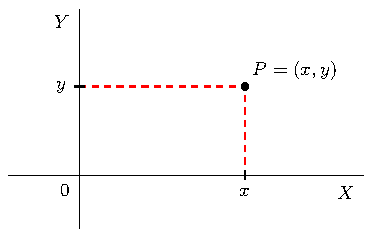
\includegraphics{figuras/plano-cartesiano.pdf}
        \caption{Plano cartesiano}
        \label{fig:plano-cartesiano}
    \end{figure}

    \par\avoidorphan{6}\subsection*{Ejercicios}

    \begin{ejercicio}\label{ej:4}
        Sean $A=\{0,1,2,3,4,5,6,7,8,9\}$, $B=\{5,6,7,8,9\}$, $C=\{0,1,2,3,4\}$,
        $D=\{3,4,5\}$ y $E=\{a,e,i,o,u\}$ y $F=\{a,e,o\}$. Calcula
        lo siguiente:
        \begin{multicols}{2}
        \begin{enumerate}[nosep]
            \item $A\cup B$, $B\cup C$ y $D\cup F$.
            \item $A\cap B$, $B\cap C$ y $D\cap F$.
            \item $B\cup C\cup D$ y $B\cap C\cap D$.
            \item $B\cup D\cup E$ y $B\cap D\cap E$.
            \item $A\backslash B$, $B\backslash A$, $B\backslash C$ y $A\backslash D$.
            \item $A\backslash E$, $E\backslash A$, $E\backslash F$ y $F\backslash E$.
        \end{enumerate}
        \end{multicols}
    \end{ejercicio}

    \begin{ejercicio}\label{ej:5}
        Encuentra $\cup_{n=1}^{\infty}A_{n}$ y $\cap_{n=1}^{\infty}A_{n}$ si $A_{n}=\{1,2,\ldots,n\}$ para cada
        $n\in\N$.
    \end{ejercicio}

    \begin{ejercicio}\label{ej:6}
        Encuentra $\cup_{n=1}^{\infty}A_{n}$ y $\cap_{n=1}^{\infty}A_{n}$ si $A_{n}=\{n,n+1,n+2,\ldots\}$ para
        cada $n\in\N$.
    \end{ejercicio}

    \begin{ejercicio}[El producto cruz de dos conjuntos no es conmutativo]\label{ej:7}
        Muestra un par de conjuntos $A$ y $B$ tales que $A\times B\neq B\times A$.
    \end{ejercicio}

    \begin{ejercicio}\label{ej:8}
        Prueba los incisos (b), (c) y (d) de la proposición~\ref{prop:2}.
    \end{ejercicio}

    \begin{ejercicio}\label{ej:9}
        Prueba la proposición~\ref{prop:3}.
    \end{ejercicio}

    \chapter{Los Números Reales}\label{cap:reales}

    En este trabajo supondremos la existencia del conjunto $\R$ de los \textit{números
    reales}\index{numeros reales@números reales}. Una de las razones de nuestro estudio de los números reales es que el
    dominio y codominio de las funciones que estudiaremos en el capítulo~\ref{cap:funciones} serán
    subconjuntos de $\R$. Recordemos que el conjunto de los números naturales es
    el conjunto
    \begin{equation*}
        \N=\{1,2,3,4,\ldots\}.
    \end{equation*}
    Definimos el conjunto de los \textit{números enteros}\index{numeros enteros@números enteros} como el conjunto
    \begin{equation*}
        \Z=\{\ldots,-3,-2,-1,0,1,2,3,\ldots\},
    \end{equation*}
    el conjunto de los \textit{números racionales}\index{numeros racionales@números racionales} como el conjunto
    \begin{equation*}
        \Q=\{a/b:a,b\in\Z\text{ con }b\neq 0\},
    \end{equation*}
    y el conjunto de los \textit{números irracionales}\index{numeros irracionales@números irracionales} como el conjunto
    \begin{equation*}
        \I=\R\backslash\Q,
    \end{equation*}
    es decir, el conjunto de los números irracionales es el conjunto de todos los
    números reales que no son racionales. Más adelante probaremos la existencia
    de números irracionales. Notemos que
    \begin{equation*}
        \N\subset\Z\subset\Q\subset\R,\ \ \I\subset\R,\ \ \R=\Q\cup\I\ \text{ y }\ \Q\cap\I=\emptyset.
    \end{equation*}

    De aquí en adelante, a menos que se indique lo contrario, trabajaremos
    con subconjuntos de $\R$ y de $\R^{2}$, en consecuencia, en lugar de expresar conjuntos
    como $\{x\in\R:P(x)\}$ o $\{(x,y)\in\R^{2}:P(x,y)\}$ escribiremos simplemente
    $\{x:P(x)\}$ o $\{(x,y):P(x,y)\}$.

    \section{Axiomas de los Números Reales}

    En esta sección estudiaremos los axiomas de los números reales y algunas
    de sus consecuencias.

    \subsection{Axiomas de la Suma y del Producto}\label{subsec:axiomas-suma}\index{axiomas de la suma y del producto}

    En $\R$ existen dos operaciones, la \textit{suma o adición}\index{suma de numeros reales@suma de números reales}\index{adicion de numeros reales@adición de números reales} «$+$» y el \textit{producto o
    multiplicación}\index{producto de numeros reales@producto de números reales}\index{multiplicacion de numeros reales@multiplicación de números reales} «$\cdot$» que cumplen los axiomas siguientes. En lo que sigue, $x$, $y$
    y $z$ son números reales.
    \begin{enumerate}[label=\arabic*.,series=axiomas]
        \item \textbf{Conmutatividad de la suma:}
        \begin{equation*}
            x+y=y+x.
        \end{equation*}
        \item \textbf{Asociatividad de la suma:}
        \begin{equation*}
            x+(y+z)=(x+y)+z.
        \end{equation*}
        \item \textbf{Existencia del neutro aditivo:} Existe un número real, denotado por $0$,
        tal que
        \begin{equation*}
            x+0=x.
        \end{equation*}
        \item \textbf{Existencia de inversos aditivos:} Dado $x\in\R$, existe un número real,
        llamado el \textit{inverso aditivo}\index{inverso aditivo de un numero real@inverso aditivo de un número real} de $x$ y denotado por $-x$, tal que
        \begin{equation*}
            x+(-x)=0.
        \end{equation*}
        \item \textbf{Conmutatividad del producto:}
        \begin{equation*}
            x\cdot y=y\cdot x.
        \end{equation*}
        \item \textbf{Asociatividad del producto:}
        \begin{equation*}
            x\cdot(y\cdot z)=(x\cdot y)\cdot z.
        \end{equation*}
        \item \textbf{Existencia del neutro multiplicativo:} Existe un número real distinto
        de $0$, denotado por $1$, tal que
        \begin{equation*}
            x\cdot 1=x.
        \end{equation*}
        \item \textbf{Existencia de inversos multiplicativos:} Dado $x\in\R$ con $x\neq 0$, existe
        un número real llamado el \textit{inverso multiplicativo}\index{inverso multiplicativo de un numero real@inverso multiplicativo de un número real} de $x$ y denotado por $x^{-1}$
        tal que
        \begin{equation*}
            x\cdot x^{-1}=1.
        \end{equation*}
        \item \textbf{Distributividad:}
        \begin{equation*}
            x\cdot(y+z)=x\cdot y+x\cdot z.
        \end{equation*}
    \end{enumerate}

    Notemos que los primeros cuatro axiomas se refieren a la suma, los cuatro
    siguientes al producto, y el último relaciona ambas operaciones.

    Otros símbolos que usaremos para el producto $x\cdot y$ son $xy$, $x(y)$, $(x)y$ y
    $(x)(y)$. También se suelen usar corchetes o llaves en lugar de paréntesis.

    Pareciera que es ocioso y aburrido estudiar propiedades tan simples como
    los axiomas de los números reales, sin embargo, como se verá en las próximas
    secciones, a partir de tales axiomas obtendremos resultados nada evidentes
    y complejos, los cuales usaremos en lo que resta del texto.

    \begin{observacion}\label{obs:2}
        En principio, la operación «$+$» solo nos permite sumar dos
        números reales. Si deseamos sumar, por ejemplo, tres números reales $x$, $y$
        y $z$, tenemos dos candidatos para tal suma, uno es $x+(y+z)$ y el otro es
        $(x+y)+z$. La asociatividad de la suma nos dice que estos dos números son
        iguales, así que definimos $x+y+z$ como $x+(y+z)$ o como $(x+y)+z$.
        Procedemos de manera similar si deseamos sumar cuatro o más números
        reales. Un tratamiento similar se tiene para el producto de tres o más números
        reales.
    \end{observacion}

    Definimos ahora a la resta o sustracción y el cociente o división de dos
    números reales.

    \begin{definicion}[Resta y división de números reales]\label{def:8}\label{def:resta-division}
        Sean $x$ y $y$ números reales.
        \begin{enumerate}
            \item Definimos la \textit{resta o sustracción}\index{resta de numeros reales@resta de números reales}\index{sustraccion de numeros reales@sustracción de números reales} de $x$ menos $y$ como
            \begin{equation*}
                x-y=x+(-y).
            \end{equation*}
            \item Si $x\neq 0$, definimos el \textit{cociente o división}\index{cociente de numeros reales@cociente de números reales}\index{division de numeros reales@división de números reales} de $y$ entre $x$ como
            \begin{equation*}
                \frac{y}{x}=y\cdot x^{-1}.
            \end{equation*}
            Otros símbolos para la división son $y/x$ y $y\entre x$.
        \end{enumerate}
    \end{definicion}

    Un primer resultado de los axiomas de los números reales son las leyes de
    cancelación para la suma y para el producto, las cuales hemos usado desde
    nuestros cursos de álgebra elemental para «despejar» una variable en una
    ecuación.

    \begin{proposicion}[Leyes de cancelación]\label{prop:4}
        \index{leyes de cancelacion@leyes de cancelación}
        \begin{enumerate}
            \item Ley de cancelación para la suma\index{ley de cancelacion para la suma@ley de cancelación para la suma}:
            \begin{equation*}
                \text{Si }x+y=z,\text{ entonces }y=z-x.
            \end{equation*}
            \item Ley de cancelación para el producto\index{ley de cancelacion para el producto@ley de cancelación para el producto}:
            \begin{equation*}
                \text{Si }x\neq 0\text{ y }xy=z,\text{ entonces }y=\frac{z}{x}.
            \end{equation*}
        \end{enumerate}
    \end{proposicion}

    \begin{proof}
        (a) Notemos que
        \begin{align*}
            &x+y=z\\
            \Rightarrow{}& -x+(x+y)=-x+z &&\text{(sumamos $-x$ a ambos miembros de la igualdad)}\\
            \Rightarrow{}& (-x+x)+y=-x+z &&\text{(asociatividad de la suma)}\\
            \Rightarrow{}& 0+y=-x+z &&\text{(propiedad de $-x$)}\\
            \Rightarrow{}& y=-x+z &&\text{(propiedad del $0$)}\\
            \Rightarrow{}& y=z+(-x) &&\text{(conmutatividad de la suma)}\\
            \Rightarrow{}& y=z-x. &&\text{(definición de la resta)}
        \end{align*}
        La demostración del inciso (b) se deja a cargo del lector (véase el ejercicio~\ref{ej:10}).
    \end{proof}

    En el inciso (a) de la proposición anterior comúnmente decimos que como la $x$ está
    sumando, pasa al otro miembro de la ecuación restando. De
    manera similar, en el inciso (b) comúnmente decimos que como la $x$ está
    multiplicando, pasa al otro miembro de la ecuación dividiendo.

    Ahora mostraremos la unicidad de los neutros aditivo y multiplicativo y
    de los inversos aditivo y multiplicativo.

    \begin{proposicion}[Unicidad de los neutros aditivo y multiplicativo]\label{prop:5}
        \begin{enumerate}
            \item El $0$ es el único número real con la propiedad de que $x+0=x$ para todo
            $x\in\R$.
            \item El $1$ es el único número real con la propiedad de que $x\cdot 1=x$ para todo
            $x\in\R$.
        \end{enumerate}
    \end{proposicion}

    \begin{proof}
        (a) Supongamos que el número $y$ cumple que $x+y=x$ para
        todo $x\in\R$. Notemos que
        \begin{align*}
            &x+y=x\\
            \Rightarrow{}& y=x-x &&\text{(ley de cancelación para la suma)}\\
            \Rightarrow{}& y=0. &&\text{(propiedad de $-x$)}
        \end{align*}
        La demostración del inciso (b) se deja a cargo del lector (véase el ejercicio~\ref{ej:11}).
    \end{proof}

    \begin{proposicion}[Unicidad de los inversos aditivo y multiplicativo]\label{prop:6}
        \begin{enumerate}
            \item Dado $x\in\R$, el número $-x$ es el único número real que satisface que
            $x+(-x)=0$.
            \item Dado $x\in\R$ con $x\neq 0$, el número $x^{-1}$ es el único número real que satisface
            que $x\cdot x^{-1}=1$.
        \end{enumerate}
    \end{proposicion}

    \begin{proof}
        (a) Sea $x\in\R$. Supongamos que el número $y$ cumple que
        $x+y=0$. Notemos que
        \begin{align*}
            &x+y=0\\
            \Rightarrow{}& y=0-x &&\text{(ley de cancelación para la suma)}\\
            \Rightarrow{}& y=-x. &&\text{(propiedad del $0$)}
        \end{align*}
        La demostración del inciso (b) se deja a cargo del lector (véase el ejercicio~\ref{ej:12}).
    \end{proof}

    Continuamos esta subsección con la proposición siguiente que nos será de
    utilidad, entre otras cosas, para mostrar el porqué no se puede dividir por
    cero.

    \begin{proposicion}\label{prop:7}
        Para todo número real $x$ se cumple que
        \begin{equation*}
            0\cdot x=0.
        \end{equation*}
    \end{proposicion}

    \begin{proof}
        Por la distributividad y por la propiedad del $0$ tenemos que
        \begin{equation*}
            0\cdot x+0\cdot x=(0+0)\cdot x=0\cdot x.
        \end{equation*}
        Así,
        \begin{equation*}
            0\cdot x+0\cdot x=0\cdot x.
        \end{equation*}
        Luego, por la ley de cancelación para la suma resulta que $0\cdot x=0\cdot x-0\cdot x=0$.
    \end{proof}

    \begin{observacion}[¿Por qué no se puede dividir por cero?]\label{obs:3}
        Llegamos a
        uno de los puntos que más confusión causa en el mundo, y es el planteado
        por la pregunta anterior. Muchas personas nacen, se desarrollan, se divierten
        y finalmente se mueren sin saber el porqué no se puede dividir por cero. La
        razón es la siguiente:

        Supongamos que se puede dividir por cero, es decir, que existe $0^{-1}$, el
        inverso multiplicativo de $0$. Luego, por la proposición~\ref{prop:7} y por la propiedad
        de los inversos multiplicativos obtenemos que
        \begin{equation*}
            0=0\cdot 0^{-1}=1,
        \end{equation*}
        lo cual es imposible. Por lo tanto, no se puede dividir por cero.
    \end{observacion}

    \subsection{Axiomas de Orden}\label{subsec:axiomas-orden}\index{axiomas de orden}

    Además de las operaciones de suma y multiplicación, tenemos una relación
    de orden «$<$» entre dos números reales que cumple los axiomas siguientes
    (la expresión $x<y$ se lee «$x$ menor que $y$» o «$x$ es menor que $y$»):\footnote{Geométricamente, $x<y$ significa que si situamos sobre la recta numérica a $x$ y a $y$,
    entonces $x$ está a la izquierda de $y$.}
    \begin{enumerate}[resume*=axiomas]
        \item \textbf{Tricotomía:} Dados $x$ y $y$ números reales, se cumple una y solo una de las
        condiciones siguientes:
        \begin{equation*}
            x<y,\quad x=y,\quad y<x.
        \end{equation*}
        \item \textbf{Transitividad:} Dados $x$, $y$ y $z$ números reales,
        \begin{equation*}
            \text{si }x<y\text{ y }y<z,\text{ entonces }x<z.
        \end{equation*}
        \item \textbf{Preservación del orden bajo la suma:} Dados $x$, $y$ y $z$ números reales,
        \begin{equation*}
            \text{si }x<y,\text{ entonces }x+z<y+z.
        \end{equation*}
    \end{enumerate}

    Antes de enunciar el último axioma sobre el orden de los números reales
    necesitamos la definición siguiente.

    \begin{definicion}[Números positivos y números negativos]\label{def:9}\label{def:positivos}
        Sea $x$ un número real.
        \begin{enumerate}
            \item Diremos que $x$ es \textit{positivo}\index{numeros positivos@números positivos} si $0<x$.
            \item Diremos que $x$ es \textit{negativo}\index{numeros negativos@números negativos} si $x<0$.
        \end{enumerate}
    \end{definicion}

    Provistos de la definición anterior, enunciamos el axioma siguiente.
    \begin{enumerate}[resume*=axiomas]
        \item \textbf{Preservación del orden bajo el producto por números positivos:}
        Dados $x$, $y$ y $z$ números reales,
        \begin{equation*}
            \text{si }x<y\text{ y }z\text{ es positivo, entonces }xz<yz.
        \end{equation*}
    \end{enumerate}

    Al igual que con los axiomas para la suma y el producto, a partir de los
    axiomas para el orden «$<$» obtendremos resultados importantes, los cuales
    usaremos en lo que resta del texto.

    Además de la relación de orden «$<$», definimos las relaciones siguientes.

    \begin{definicion}\label{def:10}\label{def:mayor-que}
        En lo que sigue $x$, $y$ y $z$ son números reales.
        \begin{enumerate}
            \item Definimos $x>y$ si $y<x$.
            \item Definimos $x\leq y$ si $x<y$ o $x=y$.
            \item Definimos $x\geq y$ si $y\leq x$.
        \end{enumerate}
    \end{definicion}

    La expresión $x>y$ se lee «$x$ mayor que $y$» o «$x$ es mayor que $y$». La
    expresión $x\leq y$ se lee «$x$ menor o igual que $y$» o «$x$ es menor o igual que $y$».
    Finalmente, la expresión $x\geq y$ se lee «$x$ mayor o igual que $y$» o «$x$ es mayor
    o igual que $y$».

    Por ejemplo, aunque tal vez sea ocioso, es correcto escribir $5\leq 5$ y $7\leq 9$.

    La primera consecuencia que veremos de los axiomas de orden es la siguiente.

    \begin{proposicion}\label{prop:8}
        Sean $x$ y $y$ números reales. Entonces
        \begin{equation*}
            x<y\text{ si y sólo si }y-x>0.
        \end{equation*}
    \end{proposicion}

    \begin{proof}
        Por la preservación del orden bajo la suma obtenemos que
        \begin{align*}
            &x<y\\
            \Rightarrow{}& x-x<y-x\\
            \Rightarrow{}& 0<y-x. &&\text{(por la propiedad de $-x$)}
        \end{align*}
        Es fácil ver que las implicaciones contrarias en las desigualdades anteriores
        también se cumplen, por lo cual obtenemos lo afirmado.
    \end{proof}

    Ahora veremos que si multiplicamos ambos miembros de una desigualdad
    por un número negativo, la desigualdad se invierte.

    \begin{proposicion}[Inversión del orden bajo el producto por números negativos]\label{prop:9}
        Sean $x$, $y$ y $z$ números reales.
        \begin{equation*}
            \text{Si }x<y\text{ y }z\text{ es negativo, entonces }xz>yz.
        \end{equation*}
    \end{proposicion}

    \begin{proof}
        Supongamos que $x<y$ y que $z<0$. Por la proposición~\ref{prop:8}
        sabemos que $y-x>0$. Luego, por la preservación del orden bajo el producto
        por números positivos resulta que
        \begin{align*}
            &z<0\\
            \Rightarrow{}& (y-x)z<(y-x)0\\
            \Rightarrow{}& yz-xz<0 &&\text{(por la distributividad y la propiedad del $0$)}\\
            \Rightarrow{}& yz-xz+xz<xz &&\text{(sumamos $xz$ a ambos lados)}\\
            \Rightarrow{}& yz+(-xz+xz)<xz &&\text{(asociatividad de la suma)}\\
            \Rightarrow{}& yz+0<xz &&\text{(propiedad de $-xz$)}\\
            \Rightarrow{}& yz<xz, &&\text{(propiedad del $0$)}
        \end{align*}
        que es lo que deseábamos probar.
    \end{proof}

    La proposición siguiente determina el signo (positivo o negativo) del producto
    de dos números distintos de cero y complementa al ejercicio~\ref{ej:14} (leyes
    de los signos para la multiplicación).

    \begin{proposicion}\label{prop:10}
        Sean $x$, $y$ y $z$ números reales.
        \begin{enumerate}[nosep]
            \item Si $x>0$ y $y>0$, entonces $xy>0$.
            \item Si $x<0$ y $y<0$, entonces $xy>0$.
            \item Si $x>0$ y $y<0$, entonces $xy<0$.
            \item Si $x<0$ y $y>0$, entonces $xy<0$.
        \end{enumerate}
    \end{proposicion}

    \begin{proof}
        (a) Supongamos que $x>0$ y $y>0$. Por la preservación del
        orden bajo el producto por números positivos obtenemos que
        \begin{align*}
            &0<x\\
            \Rightarrow{}& 0\cdot y<x\cdot y &&\text{(al multiplicar por $y>0$)}\\
            \Rightarrow{}& 0<x\cdot y, &&\text{(por la propiedad del $0$)}
        \end{align*}
        que es lo que queríamos probar.

        (b) Supongamos que $x<0$ y $y<0$. Por la proposición~\ref{prop:9} obtenemos que
        \begin{align*}
            &x<0\\
            \Rightarrow{}& x\cdot y>0\cdot y &&\text{(al multiplicar por $y<0$)}\\
            \Rightarrow{}& x\cdot y>0, &&\text{(por la propiedad del $0$)}
        \end{align*}
        que es lo que queríamos probar.

        Las demostraciones de los incisos (c) y (d) se dejan a cargo del lector (véase
        el ejercicio~\ref{ej:26}).
    \end{proof}

    \begin{definicion}[Potencias enteras]\label{def:11}
        \footnote{En el ejercicio~\ref{ej:39} definiremos las potencias racionales y en \cite{nunez2020calculoII} las potencias reales.}Sean $x$ un número real y $n$ un número natural.
        \begin{enumerate}[nosep]
            \item Definimos $x^{0}=1$, $x^{1}=x$ y para $n\geq 2$ definimos $x^{n}$ como el producto de
            $x$ consigo mismo $n$ veces.
            \item Si $x\neq 0$, definimos $x^{-n}$ ya sea como $(x^{n})^{-1}$ o como $(x^{-1})^{n}$ (véase el
            ejercicio~\ref{ej:21}).
        \end{enumerate}
    \end{definicion}

    Continuamos esta subsección con la proposición siguiente que nos será de
    utilidad, entre otras cosas, para mostrar el porqué no se puede sacar la raíz
    cuadrada de números negativos.

    \begin{proposicion}\label{prop:11}
        Para todo número real $x\neq 0$ se cumple que
        \begin{equation*}
            x^{2}>0.
        \end{equation*}
    \end{proposicion}

    \begin{proof}
        Procederemos por casos.

        Caso 1. $x>0$. En este caso, por el inciso (a) de la proposición~\ref{prop:10}, $x^{2}=x\cdot x>0$.

        Caso 2. $x<0$. En este caso, por el inciso (b) de la proposición~\ref{prop:10}, $x^{2}=x\cdot x>0$.
    \end{proof}

    A continuación, como consecuencia de la proposición~\ref{prop:11}, mostraremos que
    no existe la raíz cuadrada de un número negativo. Recordemos primero la
    definición de la raíz cuadrada.

    En aritmética se define una \textit{raíz cuadrada}\index{raiz cuadrada@raíz cuadrada} de un número $x$ como un número
    $y$ tal que $y^{2}=x$. Notemos que si $y$ es una raíz cuadrada de $x$, entonces $-y$
    también lo es, pues $(-y)^{2}=y^{2}=x$. Por ejemplo, una raíz cuadrada de $9$ es
    $3$, pues $3^{2}=9$, y otra es $-3$, pues $(-3)^{2}=9$. De aquí en adelante, cuando
    hagamos referencia a la raíz cuadrada de un número $x$ nos referiremos a la
    raíz cuadrada no negativa de $x$, la cual denotaremos por $\sqrt{x}$ o por $x^{1/2}$. Más
    adelante, en la sección~\ref{sec:racionales}, probaremos que $\sqrt{x}$ existe para todo $x\geq 0$.\footnote{Con los trece axiomas de los números reales que hemos visto hasta ahora no se puede
    probar que $\sqrt{x}$ existe para todo $x\geq 0$; se requiere de un nuevo axioma, el axioma del
    supremo, que estudiaremos en la próxima subsección.} En
    la observación siguiente mostramos que $\sqrt{x}$ no existe si $x<0$.

    \begin{observacion}[¿Por qué no se puede extraer la raíz cuadrada de números negativos?]\label{obs:4}
        Al igual que con la división por cero, la pregunta
        anterior es causa de confusión entre algunos estudiantes. La razón por la cual
        no se puede extraer la raíz cuadrada a números negativos es la siguiente:

        Si $x<0$ y suponemos que $y$ es la raíz cuadrada de $x$, entonces, por la
        proposición~\ref{prop:11}, obtenemos que
        \begin{equation*}
            0\leq y^{2}=x<0,
        \end{equation*}
        lo cual no es posible. Por lo tanto, no existe la raíz cuadrada de números
        negativos.\footnote{La raíz cuadrada de un número negativo no existe como número real, sin embargo, si
        existe como un número complejo. El lector interesado en los números complejos puede ver,
        por ejemplo, \cite{nunez2020variable}.}
    \end{observacion}

    En general, dado un número natural $n$, se define una \textit{raíz $n$-ésima}\index{raiz n-esima@raíz $n$-ésima} de un
    número $x$ como un número $y$ tal que $y^{n}=x$. Por ejemplo, la raíz cúbica de
    $8$ es $2$, pues $2^{3}=8$. Notemos que si $n$ es par\footnote{Recordemos que un número $m$ es par si $m=2k$ para algún número entero $k$, e impar si
    $m=2k+1$ para algún número entero $k$.} y $y$ es una raíz $n$-ésima de $x$,
    entonces $-y$ también lo es. Por otra parte, si $n$ es impar y $y$ es una raíz $n$-ésima
    de $x$, entonces esta es única (véase el ejercicio~\ref{ej:36}). De aquí en adelante,
    cuando $n$ sea par y hagamos referencia a la raíz $n$-ésima de un número $x$ nos
    referiremos a la raíz $n$-ésima no negativa de $x$, la cual denotaremos por $\sqrt[n]{x}$ o
    por $x^{1/n}$. Si $n$ es impar, $\sqrt[n]{x}$ o $x^{1/n}$ denotará a la raíz $n$-ésima del número $x$.
    Más adelante, en la sección~\ref{sec:racionales}, trataremos la existencia de raíces $n$-ésimas,
    por lo pronto, de manera similar al caso de la raíz cuadrada (caso $n=2$), si
    $x<0$ y $n$ es par, entonces no existe la raíz $n$-ésima de $x$.

    Las relaciones de orden «$<$» y «$\leq$» permiten definir un tipo especial
    de subconjuntos de $\R$ a los que llamaremos intervalos. Tales conjuntos los
    usaremos a lo largo del texto.

    \begin{definicion}[Intervalos]\label{def:12}\index{intervalos de numeros reales@intervalos de números reales}
        Sean $a$ y $b$ números reales.
        \begin{enumerate}
            \item Definimos\footnote{La notación $a<x<b$ significa que $a<x$ y $x<b$. Interpretaciones similares se tienen
            para expresiones como $a\leq x\leq b$, $a<x\leq b$ y $a\leq x<b$.}
            \begin{align*}
                (a,b)&=\{x:a<x<b\},\\
                [a,b]&=\{x:a\leq x\leq b\},\\
                (a,b]&=\{x:a<x\leq b\},\\
                [a,b)&=\{x:a\leq x<b\}.
            \end{align*}
            Al conjunto $(a,b)$ se le llama \textit{intervalo abierto}\index{intervalo abierto}, al conjunto $[a,b]$ \textit{intervalo
            cerrado}\index{intervalo cerrado}, al conjunto $(a,b]$ \textit{intervalo semiabierto}\index{intervalo semiabierto} por la izquierda y semicerrado
            por la derecha y al conjunto $[a,b)$ \textit{intervalo semicerrado}\index{intervalo semicerrado} por la
            izquierda y semiabierto por la derecha (todos ellos con extremos $a$ y $b$).
            \item También definimos a los \textit{intervalos infinitos}\index{intervalos infinitos}
            \begin{align*}
                (a,\infty)&=\{x:a<x\},\\
                [a,\infty)&=\{x:a\leq x\},\\
                (-\infty,a)&=\{x:x<a\},\\
                (-\infty,a]&=\{x:x\leq a\},\\
                (-\infty,\infty)&=\R.
            \end{align*}
            A los intervalos de la forma $(a,\infty)$, $(-\infty,a)$ y $(-\infty,\infty)$ también les llamaremos
            intervalos abiertos (infinitos); a los intervalos de la forma $[a,\infty)$,
            $(-\infty,a]$ y $(-\infty,\infty)$ también les llamaremos intervalos cerrados (infinitos).
        \end{enumerate}
    \end{definicion}

    Notemos que si $b<a$, entonces $(a,b)=[a,b]=(a,b]=[a,b)=\emptyset$. Notemos
    también que $(a,a)=(a,a]=[a,a)=\emptyset$ y que $[a,a]=\{a\}$.

    Las figuras~\ref{fig:2.1} y~\ref{fig:2.2} muestran a los intervalos de la definición anterior sobre
    la recta de los números reales en el caso en que $a<b$.

    De aquí en adelante, a menos que se indique lo contrario, cuando consideremos
    intervalos de la forma $(a,b)$, $(a,b]$ o $[a,b)$, supondremos que $a<b$; y
    cuando consideremos intervalos de la forma $[a,b]$, supondremos que $a\leq b$.

    \begin{figure}[H]
        \centering
        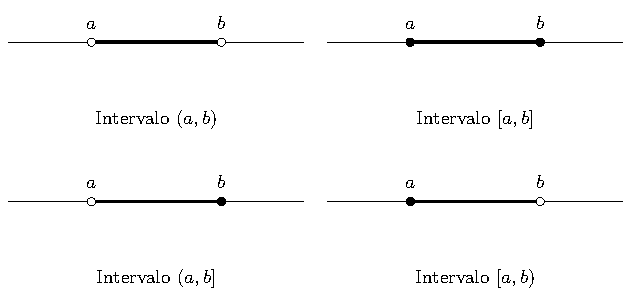
\includegraphics{figuras/intervalos-finitos.pdf}
        \caption{Intervalos finitos. En cada figura el punto vacío significa que el intervalo no
        contiene ese punto, y el punto relleno significa que si lo contiene.}
        \label{fig:2.1}
    \end{figure}

    \begin{figure}[H]
        \centering
        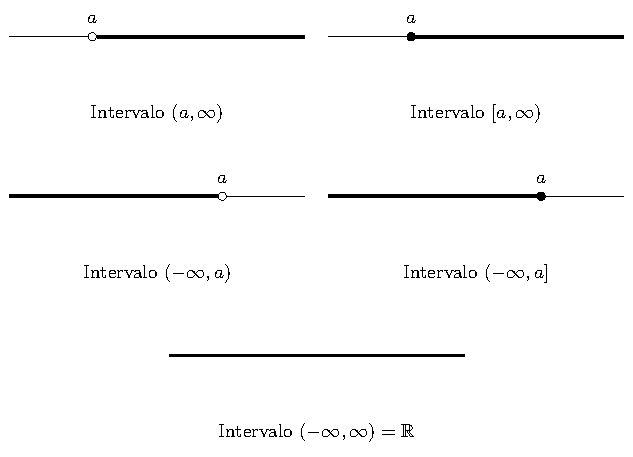
\includegraphics{figuras/intervalos-infinitos.pdf}
        \caption{Intervalos infinitos. En cada figura el punto vacío significa que el intervalo no
        contiene ese punto, y el punto relleno significa que si lo contiene. En la figura del intervalo
        $(-\infty,\infty)$ se entiende que la recta se prolonga a ambos lados indefinidamente.}
        \label{fig:2.2}
    \end{figure}

    \subsection{Axioma del Supremo}\index{axioma del supremo}

    El último, pero no menos importante, axioma de los números reales que
    estudiaremos en este curso es el axioma del supremo. Como veremos más
    adelante, el axioma del supremo tendrá implicaciones profundas, por ejemplo,
    tal axioma es necesario para probar la existencia de números irracionales,
    además, será la base para probar cuatro de los teoremas más importantes
    sobre las funciones continuas, el teorema de la función acotada (teorema~\ref{teo:1}),
    el teorema del mínimo y del máximo (teorema~\ref{teo:2}), el teorema del valor
    intermedio (teorema~\ref{teo:3}) y el teorema~\ref{teo:5} sobre continuidad uniforme.

    Para enunciar el axioma del supremo necesitaremos primero algunas definiciones.

    \begin{definicion}[Máximo y mínimo de un conjunto de números reales]\label{def:13}
        Sea $A$ un conjunto no vacío de números reales.
        \begin{enumerate}
            \item Diremos que un número $M$ es el \textit{máximo}\index{maximo de un conjunto@máximo de un conjunto} del conjunto $A$ si $M\in A$ y
            \begin{equation*}
                x\leq M\text{ para todo }x\in A.
            \end{equation*}
            Denotaremos al máximo de $A$ por $\max A$ o por $\max(A)$ para evitar confusiones.
            \item Diremos que el número $m$ es el \textit{mínimo}\index{minimo de un conjunto@mínimo de un conjunto} del conjunto $A$ si $m\in A$ y
            \begin{equation*}
                m\leq x\text{ para todo }x\in A.
            \end{equation*}
            Denotaremos al mínimo del conjunto $A$ por $\min A$ o por $\min(A)$ para
            evitar confusiones.
        \end{enumerate}
    \end{definicion}

    Por ejemplo, $\max([2,7])=7$, $\max((-\infty,0]\cup[3,4])=4$ y $\max([2,7))$ no
    existe. Es claro que el mínimo y máximo de un conjunto, cuando existen, son
    únicos.

    \begin{definicion}[Cotas superiores e inferiores]\label{def:14}
        Sea $A$ un conjunto de números reales.
        \begin{enumerate}
            \item Diremos que un número real $C$ es \textit{cota superior}\index{cota superior de un conjunto} del conjunto $A$ si
            \begin{equation*}
                x\leq C\text{ para todo }x\in A.
            \end{equation*}
            Diremos que $A$ está \textit{acotado superiormente}\index{conjunto acotado superiormente} si $A$ tiene una cota superior.
            \item Diremos que un número real $C$ es \textit{cota inferior}\index{cota inferior de un conjunto} del conjunto $A$ si
            \begin{equation*}
                C\leq x\text{ para todo }x\in A.
            \end{equation*}
            Diremos que $A$ está \textit{acotado inferiormente}\index{conjunto acotado inferiormente} si $A$ tiene una cota inferior.
            \item Diremos que $A$ es \textit{acotado}\index{conjunto acotado} si $A$ es acotado superiormente e inferiormente.
        \end{enumerate}
    \end{definicion}

    Por ejemplo, el número $7$ es cota superior de los conjuntos $(-\infty,5)$, $[2,7]$
    y $[2,7)$.

    Notemos que el máximo de un conjunto, cuando existe, es cota superior
    del conjunto y que el mínimo de un conjunto, cuando existe, es cota inferior
    del conjunto.

    En la próxima sección probaremos que el conjunto $\N$ de los números naturales
    no está acotado superiormente y, en consecuencia, los conjuntos $\Z$
    y $\R$ no están acotados ni superiormente ni inferiormente. Todo conjunto de
    la forma $[a,\infty)$ no está acotado superiormente y todo conjunto de la forma
    $(-\infty,a]$ no está acotado inferiormente.

    \begin{definicion}[Supremo e ínfimo]\label{def:15}
        Sea $A$ un conjunto no vacío de números reales.
        \begin{enumerate}
            \item Diremos que un número real $\alpha$ es el \textit{supremo}\index{supremo de un conjunto} del conjunto $A$ si $\alpha$ es la
            mínima cota superior de $A$, es decir, si $\alpha$ es cota superior de $A$ y $\alpha\leq C$
            para toda cota superior $C$ del conjunto $A$. Denotaremos el supremo del
            conjunto $A$ por $\sup A$ o por $\sup(A)$ para evitar confusiones.
            \item Diremos que un número real $\alpha$ es \textit{el ínfimo}\index{infimo de un conjunto@ínfimo de un conjunto} del conjunto $A$ si $\alpha$ es la máxima
            cota inferior de $A$, es decir, si $\alpha$ es cota inferior de $A$ y $\alpha\geq C$ para toda
            cota inferior $C$ del conjunto $A$. Denotaremos el ínfimo del conjunto $A$ por
            $\inf A$ o por $\inf(A)$ para evitar confusiones.
        \end{enumerate}
    \end{definicion}

    Notemos que el máximo de un conjunto, cuando existe, es el supremo del
    conjunto y que el mínimo de un conjunto, cuando existe, es el ínfimo del
    conjunto.

    Por ejemplo, el número $7$ es el supremo del conjunto $[2,7]$ y también del
    conjunto $[2,7)$. Este ejemplo nos muestra que el supremo de un conjunto no
    siempre pertenece al conjunto. El número $7$ no es el supremo del conjunto
    $(-\infty,5)$, pues $7$ es cota superior de $(-\infty,5)$, sin embargo, no es la mínima
    cota superior.

    Enunciamos finalmente el último axioma de los números reales.
    \begin{enumerate}[resume*=axiomas]
        \item \textbf{Axioma del supremo:} Todo conjunto no vacío y acotado superiormente
        de números reales tiene supremo.
    \end{enumerate}

    Como consecuencia del axioma del supremo obtenemos fácilmente la proposición
    siguiente (véase el ejercicio~\ref{ej:43}).

    \begin{proposicion}\label{prop:12}
        Todo conjunto no vacío y acotado inferiormente de números
        reales tiene ínfimo.
    \end{proposicion}

    Una propiedad del supremo que usaremos frecuentemente es la siguiente.

    \begin{proposicion}\label{prop:13}
        Sea $A$ un conjunto no vacío y acotado superiormente de
        números reales. Si $\epsilon>0$, entonces existe $x\in A$ tal que
        \begin{equation}\label{eq:prop-supremo}
            \sup(A)-\epsilon<x\leq\sup(A)
        \end{equation}
        (véase la figura~\ref{fig:2.3}).
    \end{proposicion}

    \begin{proof}
        Basta probar que existe $x\in A$ que cumple la primera desigualdad
        de \eqref{eq:prop-supremo}, pues si $x\in A$ es claro que $x\leq\sup(A)$. Supongamos que
        no existe $x\in A$ tal que $\sup(A)-\epsilon<x$. Así, para todo $x\in A$ se cumple
        que $x\leq\sup(A)-\epsilon$. En consecuencia, $\sup(A)-\epsilon$ es una cota superior del
        conjunto $A$, lo cual contradice que $\sup(A)$ es la mínima cota superior de $A$.
        Por lo tanto, existe $x\in A$ tal que $\sup(A)-\epsilon<x$.
    \end{proof}

    \begin{figure}[H]
        \centering
        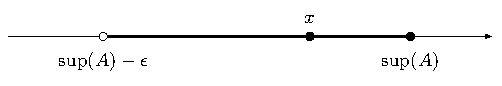
\includegraphics{figuras/propiedad-supremo.pdf}
        \caption{Propiedad del supremo de un conjunto: Si $\epsilon>0$, entonces existe $x\in A$ tal
        que $x\in(\sup(A)-\epsilon,\sup(A)]$.}
        \label{fig:2.3}
    \end{figure}

    \begin{observacion}\label{obs:5}
        El concepto de ínfimo es un concepto «dual» del concepto
        de supremo en el sentido de que si $P$ es una propiedad del supremo, entonces
        se tiene una propiedad correspondiente $P'$ para el ínfimo, y viceversa. Para
        obtener $P'$ a partir de $P$ simplemente hay que cambiar «$<$», «cota superior»,
        «acotado superiormente» y «supremo» en $P$ por «$>$», «cota inferior»,
        «acotado inferiormente» e «ínfimo», respectivamente. Por esta razón, de aquí
        en adelante, cuando expresemos una propiedad del supremo hay que tener en
        mente que se tiene una propiedad correspondiente para el ínfimo, y viceversa.
        Por ejemplo, la propiedad correspondiente a la proposición~\ref{prop:13} para el ínfimo
        es la siguiente.
    \end{observacion}

    \begin{proposicion}\label{prop:14}
        Sea $A$ un conjunto no vacío y acotado inferiormente de
        números reales. Si $\epsilon>0$, entonces existe $x\in A$ tal que
        \begin{equation*}
            \inf(A)+\epsilon>x\geq\inf(A).
        \end{equation*}
    \end{proposicion}

    \par\avoidorphan{6}\subsection*{Ejercicios}

    \subtitulo{Axiomas de la Suma y del Producto}

    \begin{ejercicio}\label{ej:10}
        Prueba el inciso (b) de la proposición~\ref{prop:4}.
    \end{ejercicio}

    \begin{ejercicio}\label{ej:11}
        Prueba el inciso (b) de la proposición~\ref{prop:5}.
    \end{ejercicio}

    \begin{ejercicio}\label{ej:12}
        Prueba el inciso (b) de la proposición~\ref{prop:6}.
    \end{ejercicio}

    \begin{ejercicio}\label{ej:13}
        Sea $x$ un número real. Prueba, usando la unicidad del inverso
        aditivo, lo siguiente:
        \begin{multicols}{2}
        \begin{enumerate}[nosep]
            \item $(-1)x=-x$.
            \item $-(-x)=x$.
        \end{enumerate}
        \end{multicols}
        \sugerencia Para probar, por ejemplo, el inciso (a) muestra primero que
        $(-1)x+x=0$ y posteriormente usa la unicidad del inverso aditivo.
    \end{ejercicio}

    El ejercicio siguiente desenmaraña uno de los misterios con el que nos
    encontramos en el curso de álgebra elemental, las leyes de los signos para
    la multiplicación. Recordemos que, dado un número real $x$, la notación $+x$
    significa lo mismo que $x$.

    \begin{ejercicio}[Leyes de los signos para la multiplicación]\label{ej:14}
        \index{leyes de los signos para la multiplicacion@leyes de los signos para la multiplicación}Prueba que
        si $x$ y $y$ son números reales, entonces
        \begin{enumerate}[nosep]
            \item $(+x)(+y)=+(xy)$.
            \item $(-x)(+y)=-(xy)$.
            \item $(+x)(-y)=-(xy)$.
            \item $(-x)(-y)=+(xy)$.
        \end{enumerate}
        Las leyes de los signos para la multiplicación se resumen de manera conveniente
        como
        \begin{align*}
            +\text{ por }+\text{ da }+\\
            -\text{ por }+\text{ da }-\\
            +\text{ por }-\text{ da }-\\
            -\text{ por }-\text{ da }+
        \end{align*}
        \sugerencia El inciso (a) es claro, pues $+x=x$, $+y=y$ y $+(xy)=xy$. Usa
        la unicidad del inverso aditivo para probar los incisos (b) y (c). Finalmente,
        deduce (d) de los incisos (b) y (c).
    \end{ejercicio}

    \begin{ejercicio}\label{ej:15}
        Sean $x$ y $y$ números reales. Prueba que si $xy=0$, entonces
        $x=0$ o $y=0$. \sugerencia Procede por contradicción.
    \end{ejercicio}

    \begin{ejercicio}\label{ej:16}
        Sea $x$ un número real distinto de cero. Prueba, usando la unicidad
        del inverso multiplicativo, que
        \begin{equation*}
            (x^{-1})^{-1}=x.
        \end{equation*}
    \end{ejercicio}

    \begin{ejercicio}\label{ej:17}
        Sean $x$ y $y$ números reales distintos de cero. Prueba, usando
        la unicidad del inverso multiplicativo, que
        \begin{equation*}
            (xy)^{-1}=x^{-1}y^{-1}.
        \end{equation*}
    \end{ejercicio}

    \begin{ejercicio}\label{ej:18}
        Sea $x$ un número real distinto de cero. Prueba, usando la unicidad
        del inverso multiplicativo o el ejercicio~\ref{ej:17}, que
        \begin{equation*}
            (-x)^{-1}=-(x^{-1}).
        \end{equation*}
    \end{ejercicio}

    \begin{ejercicio}[Aritmética de las fracciones]\label{ej:19}
        \index{aritmetica de las fracciones@aritmética de las fracciones}Sean $x$, $y$, $z$ y $w$ números
        reales tales que las expresiones algebraicas de los incisos siguientes están
        definidas. Prueba lo siguiente:
        \begin{enumerate}[nosep]
            \item $\frac{x}{y}+\frac{z}{w}=\frac{wx+yz}{yw}$.
            \item $\frac{x}{y}-\frac{z}{w}=\frac{wx-yz}{yw}$.
            \item $\frac{x}{y}\cdot\frac{z}{w}=\frac{xz}{yw}$.
            \item $\frac{x}{y}\entre\frac{z}{w}=\frac{xw}{yz}$.
        \end{enumerate}
        \sugerencia Recuerda como se definió la resta y la división de números
        reales.
    \end{ejercicio}

    \begin{ejercicio}[Leyes de los signos para la división]\label{ej:20}
        \index{leyes de los signos para la division@leyes de los signos para la división}Prueba que si $x$ y
        $y$ son números reales, con $y\neq 0$, entonces
        \begin{enumerate}[nosep]
            \item $\frac{+x}{+y}=+\frac{x}{y}$.
            \item $\frac{-x}{+y}=-\frac{x}{y}$.
            \item $\frac{+x}{-y}=-\frac{x}{y}$.
            \item $\frac{-x}{-y}=+\frac{x}{y}$.
        \end{enumerate}
        Las leyes de los signos para la división se resumen de manera conveniente
        como
        \begin{align*}
            +\text{ entre }+\text{ da }+\\
            -\text{ entre }+\text{ da }-\\
            +\text{ entre }-\text{ da }-\\
            -\text{ entre }-\text{ da }+
        \end{align*}
        \textbf{Sugerencia 1:} El inciso (a) es claro, pues $+x=x$, $+y=y$ y $+(x/y)=
        x/y$. Usa la unicidad del inverso aditivo para probar los incisos (b) y (c).
        Finalmente, deduce (d) de los incisos (b) y (c). \textbf{Sugerencia 2:} Para probar
        (b), usa las leyes de los signos para la multiplicación, y para probar (c), usa
        que $(-y)^{-1}=-(y^{-1})$ y las leyes de los signos para la multiplicación.
    \end{ejercicio}

    \begin{ejercicio}[Potencias enteras negativas]\label{ej:21}
        Sean $x\neq 0$ y $n$ un número
        natural. Usa la unicidad del inverso multiplicativo para probar que
        \begin{equation*}
            (x^{n})^{-1}=(x^{-1})^{n}.
        \end{equation*}
        En vista de esta ecuación se define $x^{-n}$ como $(x^{n})^{-1}$ o como $(x^{-1})^{n}$.
    \end{ejercicio}

    \begin{ejercicio}[Leyes de los exponentes]\label{ej:22}
        \index{leyes de los exponentes}Sean $x$ y $y$ números reales, y
        $m$ y $n$ números naturales tales que las expresiones algebraicas de los incisos
        siguientes están definidas. Prueba lo siguiente:
        \begin{enumerate}[nosep]
            \item $x^{m}\cdot x^{n}=x^{m+n}$.
            \item $x^{m}/x^{n}=x^{m-n}$.
            \item $x^{n}\cdot y^{n}=(xy)^{n}$.
            \item $(x/y)^{n}=x^{n}/y^{n}$.
            \item $(x^{m})^{n}=x^{m\cdot n}$.
        \end{enumerate}
        \sugerencia Los incisos (a), (c) y (e) son claros. Para probar los incisos (b)
        y (d), recuerda como se definió la división y ten presente el ejercicio~\ref{ej:21}.
    \end{ejercicio}

    \begin{ejercicio}\label{ej:23}
        Prueba las leyes de los exponentes (ejercicio~\ref{ej:22}) cuando $m$
        y $n$ son números enteros. \sugerencia Recuerda que si $x\neq 0$ y $n$ es un
        número natural, el número $x^{-n}$ se define como $(x^{n})^{-1}$ o como $(x^{-1})^{n}$ (véase
        el ejercicio~\ref{ej:21}).
    \end{ejercicio}

    \subtitulo{Axiomas de Orden}

    \begin{ejercicio}\label{ej:24}
        Representa gráficamente (sobre la recta de los números reales)
        cada uno de los conjuntos dados.
        \begin{multicols}{2}
        \begin{enumerate}[nosep]
            \item $(1,8]$.
            \item $[-5,-1)^{c}$.
            \item $(-\infty,-2]$.
            \item $(1,2)\cup(2,3]$.
        \end{enumerate}
        \end{multicols}
    \end{ejercicio}

    \begin{ejercicio}\label{ej:25}
        Realiza las operaciones indicadas en los incisos siguientes. Expresa
        la respuesta en términos de intervalos.
        \begin{multicols}{2}
        \begin{enumerate}[nosep]
            \item $(-9,1]\cup(-1,5]$.
            \item $(2,5]\cup(7,9]$.
            \item $(-\infty,4]\cap(-7,0)$.
            \item $(0,3]\cap(-2,0)$.
        \end{enumerate}
        \end{multicols}
    \end{ejercicio}

    \begin{ejercicio}\label{ej:26}
        Prueba los incisos (c) y (d) de la proposición~\ref{prop:10}.
    \end{ejercicio}

    \begin{ejercicio}\label{ej:27}
        Prueba que si $x\leq y$ y $y\leq x$, entonces $x=y$.
    \end{ejercicio}

    \begin{ejercicio}\label{ej:28}
        Prueba que si $x<y$ y $z<w$, entonces $x+z<y+w$.
    \end{ejercicio}

    \begin{ejercicio}\label{ej:29}
        Prueba que si $0\leq x<y$ y $0\leq z<w$, entonces $xz<yw$.
    \end{ejercicio}

    \begin{ejercicio}\label{ej:30}
        Prueba que si $x,y\geq 0$ y $x+y=0$, entonces $x=0$ y $y=0$.
        \sugerencia Procede por contradicción.
    \end{ejercicio}

    \begin{ejercicio}\label{ej:31}
        Prueba que si $0\leq x<\epsilon$ para todo $\epsilon>0$, entonces $x=0$.
        \sugerencia Procede por contradicción.
    \end{ejercicio}

    \begin{ejercicio}\label{ej:32}
        Prueba que si $x<y+\epsilon$ para todo $\epsilon>0$, entonces $x\leq y$.
        \sugerencia Procede por contradicción.
    \end{ejercicio}

    \begin{ejercicio}\label{ej:33}
        Prueba que $1>0$. \sugerencia Considera la proposición~\ref{prop:11}.
    \end{ejercicio}

    \begin{ejercicio}\label{ej:34}
        Prueba lo siguiente:
        \begin{enumerate}[nosep]
            \item Si $x>0$, entonces $x^{-1}>0$.
            \item Si $x<0$, entonces $x^{-1}<0$.
        \end{enumerate}
        \sugerencia Procede por contradicción y ten presente el ejercicio~\ref{ej:33}.
    \end{ejercicio}

    \begin{ejercicio}\label{ej:35}
        Sea $n\in\N$ con $n\geq 2$. Prueba lo siguiente:
        \begin{enumerate}[nosep]
            \item Si $0<x<1$, entonces $x^{n}<x$.
            \item Si $1<x$, entonces $x<x^{n}$.
        \end{enumerate}
        \sugerencia Prueba primero el caso en que $n=2$.
    \end{ejercicio}

    \begin{ejercicio}[Unicidad de las raíces $n$-ésimas; inyectividad\protect\footnote{Estudiaremos a las funciones inyectivas en la sección~\ref{sec:inyectivas}.} de la función $x^{n}$ en ${[0,\infty)}$ para $n$ par y en $\R$ para $n$ impar]\label{ej:36}
        Prueba lo siguiente:
        \begin{enumerate}[nosep]
            \item Si $x,y\geq 0$, $n\in\N$ y $x^{n}=y^{n}$, entonces $x=y$.
            \item Si $x,y\in\R$, $n$ es impar y $x^{n}=y^{n}$, entonces $x=y$.
        \end{enumerate}
        \sugerencia Para el inciso (a) usa que si $n\in\N$ y $n\geq 2$, entonces
        \begin{equation*}
            x^{n}-y^{n}=(x-y)\left(x^{n-1}+x^{n-2}y+x^{n-3}y^{2}+\cdots+xy^{n-2}+y^{n-1}\right).
        \end{equation*}
        Para el inciso (b) usa el inciso (a).
    \end{ejercicio}

    \begin{ejercicio}[Inyectividad de la función raíz $n$-enésima]\label{ej:37}
        Prueba que
        si $n\in\N$ y $\sqrt[n]{x}=\sqrt[n]{y}$, entonces $x=y$. \sugerencia Usa que si $x=y$ y
        $n\in\N$, entonces $x^{n}=y^{n}$.
    \end{ejercicio}

    \begin{ejercicio}[Leyes de los radicales]\label{ej:38}
        \index{leyes de los radicales}Sean $x$ y $y$ números reales, y $m$
        y $n$ números naturales tales que las expresiones algebraicas de los incisos
        siguientes están definidas. Prueba lo siguiente:
        \begin{enumerate}[nosep]
            \item $\sqrt[n]{xy}=\sqrt[n]{x}\cdot\sqrt[n]{y}$.
            \item $\sqrt[n]{\frac{x}{y}}=\frac{\sqrt[n]{x}}{\sqrt[n]{y}}$.
            \item $\sqrt[n]{x^{m}}=(\sqrt[n]{x})^{m}$.
            \item $\sqrt[n]{\sqrt[m]{x}}=\sqrt[n\cdot m]{x}$.
        \end{enumerate}
    \end{ejercicio}

    \begin{ejercicio}[Potencias racionales]\label{ej:39}
        Prueba que el inciso (c) del ejercicio~\ref{ej:38}
        también se cumple si $m$ es un número entero, es decir, prueba que si $x$ es
        un número real, $m$ es un número entero y $n$ es un número natural tales que
        $(x^{m})^{1/n}$ y $(x^{1/n})^{m}$ están definidos, entonces
        \begin{equation*}
            (x^{m})^{\frac{1}{n}}=\left(x^{\frac{1}{n}}\right)^{m}.
        \end{equation*}
        En vista de este resultado se define $x^{m/n}$ como $(x^{m})^{1/n}$ o como $(x^{1/n})^{m}$. Así
        pues, este ejercicio nos permite definir, por ejemplo, $x^{r}$ para todo $x>0$ y
        todo número racional $r$.\footnote{En \cite{nunez2020calculoII} definiremos $x^{r}$ para todo $x>0$ y todo número real $r$.} Nótese que en el caso en que $k=m/n$ es un número
        entero, este ejercicio nos proporciona una definición alterna de $x^{k}$ además de
        la dada en la definición~\ref{def:11}, sin embargo, solo consideraremos la definición
        de $x^{k}$ dada en la definición~\ref{def:11}, pues según este ejercicio el dominio de, por
        ejemplo, $x^{4/2}$ es el intervalo $[0,\infty)$ y como sabemos, el dominio de $x^{2}$ es todo
        $\R$.
    \end{ejercicio}

    \begin{ejercicio}\label{ej:40}
        Prueba las leyes de los exponentes (ejercicio~\ref{ej:22}) cuando $m$ y
        $n$ son números racionales. \sugerencia Ten presente como se define $x^{m/n}$
        para $m$ entero y $n$ natural en el ejercicio~\ref{ej:39}.
    \end{ejercicio}

    \subtitulo{Axioma del Supremo}

    \begin{ejercicio}\label{ej:41}
        Determina si existe el supremo de los conjuntos siguientes (argumenta
        tu respuesta). En caso de que exista, calcúlalo (argumenta tu respuesta).
        Para resolver este ejercicio puedes usar la proposición~\ref{prop:17} en los
        incisos (c) y (d); la proposición~\ref{prop:18} en el inciso (e) y la proposición~\ref{prop:21} en los
        incisos (f) y (g).
        \begin{multicols}{2}
        \begin{enumerate}[nosep]
            \item $(-3,5)$.
            \item $(-3,5]$.
            \item $\N$.
            \item $(0,\infty)$.
            \item $\left\{1-\frac{1}{n}:n\in\N\right\}$.
            \item $\Q\cap\left(0,\sqrt{2}\right)$.
            \item $\I\cap(0,1)$.
        \end{enumerate}
        \end{multicols}
    \end{ejercicio}

    \begin{ejercicio}\label{ej:42}
        Sea $A$ un conjunto no vacío de números reales. Prueba que si
        $x<c$ para toda $x\in A$, entonces
        \begin{equation*}
            \sup(A)\leq c.
        \end{equation*}
    \end{ejercicio}

    \begin{ejercicio}\label{ej:43}
        Prueba la proposición~\ref{prop:12}.
    \end{ejercicio}

    \begin{ejercicio}\label{ej:44}
        Sean $A$ y $B$ conjuntos no vacíos y acotados de números reales
        tales que $A\subset B$. Prueba que
        \begin{equation*}
            \inf(B)\leq\inf(A)\leq\sup(A)\leq\sup(B).
        \end{equation*}
    \end{ejercicio}

    \begin{ejercicio}\label{ej:45}
        Sean $A$ un conjunto de números reales y $c\in\R$. Definimos
        \begin{equation*}
            cA=\{ca:a\in A\}.
        \end{equation*}
        Prueba que si $A$ es un conjunto no vacío y acotado superiormente de números
        reales, y $c\geq 0$, entonces
        \begin{equation*}
            \sup(cA)=c\sup(A).
        \end{equation*}
    \end{ejercicio}

    \begin{ejercicio}\label{ej:46}
        Sea $A$ un conjunto no vacío de números reales.
        \begin{enumerate}
            \item Prueba que si $A$ es acotado inferiormente, entonces
            \begin{equation*}
                \sup(-A)=-\inf(A).
            \end{equation*}
            \item Prueba que si $A$ es acotado superiormente, entonces
            \begin{equation*}
                \inf(-A)=-\sup(A).
            \end{equation*}
        \end{enumerate}
    \end{ejercicio}

    \begin{ejercicio}\label{ej:47}
        Sean $A$ y $B$ conjuntos de números reales. Definimos
        \begin{equation*}
            A+B=\{a+b:a\in A\text{ y }b\in B\}.
        \end{equation*}
        Prueba que si $A$ y $B$ son conjuntos no vacíos y acotados superiormente de
        números reales, entonces
        \begin{equation*}
            \sup(A+B)=\sup(A)+\sup(B).
        \end{equation*}
        \sugerencia Para probar que $\sup(A)+\sup(B)\leq\sup(A+B)$ procede de
        la manera siguiente: Dado $\epsilon>0$, por la proposición~\ref{prop:13}, existen $a\in A$ y $b\in B$
        tales que
        \begin{equation*}
            \sup(A)-\frac{\epsilon}{2}<a\leq\sup(A)
        \end{equation*}
        y
        \begin{equation*}
            \sup(B)-\frac{\epsilon}{2}<b\leq\sup(B).
        \end{equation*}
        Así,
        \begin{equation*}
            \sup(A)+\sup(B)-\epsilon<a+b\leq\sup(A+B)
        \end{equation*}
        y, en consecuencia,
        \begin{equation*}
            \sup(A)+\sup(B)-\epsilon<\sup(A+B).
        \end{equation*}
        Como $\epsilon>0$ fue arbitrario, por el ejercicio~\ref{ej:32} obtenemos que
        \begin{equation*}
            \sup(A)+\sup(B)\leq\sup(A+B).
        \end{equation*}
    \end{ejercicio}

    \begin{ejercicio}\label{ej:48}
        Sean $A$ y $B$ conjuntos de números reales. Definimos
        \begin{equation*}
            AB=\{ab:a\in A\text{ y }b\in B\}.
        \end{equation*}
        Prueba que si $A$ y $B$ son conjuntos no vacíos y acotados superiormente de
        números reales positivos, entonces
        \begin{equation*}
            \sup(AB)=\sup(A)\sup(B).
        \end{equation*}
        \sugerencia Trata de imitar la prueba del ejercicio~\ref{ej:47}.
    \end{ejercicio}

    \begin{ejercicio}[Intervalos]\label{ej:49}
        Sea $I\subset\R$. Prueba que $I$ es un intervalo ssi $I$
        cumple la condición siguiente:
        \begin{equation}\label{eq:def-intervalo}
            \text{Para todo }x,y\in I,\ \text{si }x<c<y,\ \text{entonces }c\in I.
        \end{equation}
        Así pues, podemos tomar a \eqref{eq:def-intervalo} como la definición general de intervalo.
        \sugerencia Para el regreso, trata los casos $I=\emptyset$ e $I\neq\emptyset$. Posteriormente, en
        el caso $I\neq\emptyset$, trata los subcasos $I$ acotado e $I$ no acotado. En el subcaso $I$
        acotado, considera a los números $p=\inf(I)$ y $q=\sup(I)$, y trata los casos
        en que $p$ o $q$ están o no en $I$. En el subcaso $I$ no acotado, trata los
        subsubcasos $I$ acotado inferiormente y no acotado superiormente, $I$ no acotado
        inferiormente y acotado superiormente; y finalmente, el subsubcaso en que $I$
        no es acotado inferiormente ni superiormente.
    \end{ejercicio}

    \section{Los Números Naturales}\label{sec:naturales}

    En esta sección estudiaremos algunas propiedades de los números naturales
    que usaremos más adelante, entre ellas el principio de inducción matemática,
    el cual es una herramienta muy importante, entre otras cosas, para probar la
    veracidad de afirmaciones de la forma $\forall n\in\N$, $P(n)$.

    De la definición del conjunto de los números naturales (véase, por ejemplo,
    \cite{nunez2020logica}) obtenemos lo siguiente.

    \begin{proposicion}[Principio de inducción matemática]\label{prop:15}
        \index{principio de induccion matematica@principio de inducción matemática}Sea $A\subset\N$.
        Supongamos que $A$ cumple las dos condiciones siguientes:
        \begin{enumerate}[nosep]
            \item $1\in A$.
            \item Si $k\in A$, entonces $k+1\in A$.
        \end{enumerate}
        Entonces $A=\N$.
    \end{proposicion}

    A la hipótesis del inciso (b) anterior se le conoce como hipótesis de inducción.

    El principio de inducción matemática (o simplemente «principio de inducción»
    por brevedad) se puede usar para probar que una fórmula o condición
    $P(n)$, que depende de $n$, se cumple para todo $n\in\N$. En efecto, sea
    \begin{equation*}
        A=\{n\in\N:P(n)\text{ se cumple}\}.
    \end{equation*}
    Si $A$ cumple las condiciones de los incisos (a) y (b) del principio de inducción
    matemática, entonces se tendrá que $A=\N$, lo cual implicará que la fórmula
    o condición $P(n)$ se cumple para todo $n\in\N$.

    \begin{ejemplo}\label{ejm:2}
        Prueba que para todo $n\in\N$ se cumple que
        \begin{equation}\label{eq:suma-gauss}
            1+2+\cdots+n=\frac{n(n+1)}{2}.
        \end{equation}

        \textbf{Solución.} Sea $P(n)$ la fórmula \eqref{eq:suma-gauss} y consideremos el conjunto
        \begin{equation*}
            A=\{n\in\N:P(n)\}.
        \end{equation*}
        Probaremos que el conjunto $A$ cumple las condiciones (a) y (b) del principio
        de inducción matemática. En efecto:
        \begin{enumerate}
            \item Es claro que $1\in A$, pues $1=1(1+1)/2$.
            \item Supongamos que $k\in A$. Hay que probar que $k+1\in A$. Puesto que $k\in A$,
            sabemos que
            \begin{equation*}
                1+2+\cdots+k=\frac{k(k+1)}{2}.
            \end{equation*}
            En consecuencia,
            \begin{align*}
                1+2+\cdots+k+(k+1)&=\frac{k(k+1)}{2}+(k+1)\\
                &=\frac{k(k+1)}{2}+\frac{2(k+1)}{2}\\
                &=\frac{(k+2)(k+1)}{2}\\
                &=\frac{(k+1)((k+1)+1)}{2},
            \end{align*}
            lo cual muestra que $k+1\in A$.
        \end{enumerate}
        Por el principio de inducción matemática resulta que $A=\N$, de lo cual
        obtenemos que $P(n)$, es decir, la fórmula \eqref{eq:suma-gauss}, se cumple para todo $n\in\N$.
    \end{ejemplo}

    \begin{observacion}\label{obs:6}
        En la práctica, la prueba de que una fórmula o condición
        $P(n)$ se cumple para todo $n\in\N$, utilizando el principio de inducción matemática,
        como la del ejemplo anterior, se abrevia probando los puntos siguientes:
        \begin{enumerate}[label=(\roman*),nosep]
            \item La fórmula o condición $P(n)$ se cumple para $n=1$.
            \item Si la fórmula o condición $P(n)$ se cumple para $n=k$, entonces se cumple
            para $n=k+1$.
        \end{enumerate}
    \end{observacion}

    \begin{ejemplo}\label{ejm:3}
        Prueba que para todo $n\in\N$ se cumple que
        \begin{equation}\label{eq:n-menor-2n}
            n<2^{n}.
        \end{equation}

        \textbf{Solución.} Usaremos el principio de inducción matemática.

        (i) Es claro que la fórmula \eqref{eq:n-menor-2n} se cumple para $n=1$, pues $1<2^{1}$.

        (ii) Supongamos que la fórmula \eqref{eq:n-menor-2n} se cumple para $n=k$. Probaremos
        que la fórmula \eqref{eq:n-menor-2n} se cumple para $n=k+1$. En efecto,
        \begin{align*}
            k+1&<2^{k}+1 &&\text{(por la hipótesis de inducción)}\\
            &<2^{k}+2^{k}\\
            &=2\cdot 2^{k}\\
            &=2^{k+1},
        \end{align*}
        lo cual muestra que la fórmula \eqref{eq:n-menor-2n} se cumple para $n=k+1$.

        Por lo tanto, por el principio de inducción matemática, resulta que \eqref{eq:n-menor-2n}
        se cumple para todo $n\in\N$. De manera similar obtenemos que si $m$ es un
        número natural mayor o igual a $2$, entonces para todo $n\in\N$ se cumple que
        $n<m^{n}$.
    \end{ejemplo}

    El principio de inducción matemática también se puede usar para probar
    que una fórmula o condición $P(n)$ se cumple a partir de cierto número natural
    fijo $n_{0}$. En este caso, en lugar de probar (i) y (ii) de la observación~\ref{obs:6} hay que
    probar lo siguiente (véase el ejercicio~\ref{ej:67}):
    \begin{enumerate}[label=(\roman*),nosep]
        \item La fórmula o condición $P(n)$ se cumple para $n=n_{0}$.
        \item Si la fórmula o condición $P(n)$ se cumple para $n=k\geq n_{0}$, entonces se
        cumple para $n=k+1$.
    \end{enumerate}

    \begin{ejemplo}\label{ejm:4}
        Prueba que para todo $n\in\N$ con $n\geq 4$ se cumple que
        \begin{equation}\label{eq:2n-factorial}
            2^{n}\leq n!
        \end{equation}

        \textbf{Solución.} (i) Es claro que la fórmula \eqref{eq:2n-factorial} se cumple para $n=4$, pues
        $2^{4}=16<24=4!$

        (ii) Supongamos que la fórmula \eqref{eq:2n-factorial} se cumple para $n=k\geq 4$. Probaremos
        que la fórmula \eqref{eq:2n-factorial} se cumple para $n=k+1$. En efecto,
        \begin{align*}
            2^{k+1}&=2^{k}\cdot 2\\
            &\leq k!\cdot 2 &&\text{(por la hipótesis de inducción)}\\
            &\leq k!\cdot(k+1)\\
            &=(k+1)!,
        \end{align*}
        lo cual muestra que la fórmula \eqref{eq:2n-factorial} se cumple para $n=k+1$.

        Por lo tanto, por el principio de inducción matemática, resulta que \eqref{eq:2n-factorial}
        se cumple para todo $n\in\N$ con $n\geq 4$.
    \end{ejemplo}

    Como consecuencia del principio de inducción matemática obtenemos el
    resultado siguiente.

    \begin{proposicion}[Principio del buen orden]\label{prop:16}
        \index{principio del buen orden}Todo conjunto no vacío de
        números naturales tiene un elemento mínimo, es decir, dado $A\subset\N$ no vacío,
        existe $m\in A$ tal que
        \begin{equation*}
            m\leq n\text{ para todo }n\in A.
        \end{equation*}
    \end{proposicion}

    \begin{proof}
        Procederemos por contradicción. Supongamos que existe un
        conjunto no vacío $A$ de números naturales que no tiene elemento mínimo.
        Definamos
        \begin{equation*}
            B=\{n\in\N:\text{si }m\leq n,\text{ entonces }m\notin A\}.
        \end{equation*}
        Probaremos, usando el principio de inducción matemática, que $B=\N$ y, en
        consecuencia, tendremos que $A=\emptyset$, lo cual es una contradicción.

        (a) Como $1$ es el mínimo de $\N$ (véase el ejercicio~\ref{ej:51}) y $A$ no tiene elemento
        mínimo, entonces $1\notin A$. En consecuencia, $1\in B$.

        (b) Supongamos que $k\in B$. Así, $1,2,\ldots,k\notin A$ y, en consecuencia,\footnote{El símbolo $C\coloneqq\{k+1,k+2,k+3,\ldots\}$ significa que estamos definiendo al conjunto $C$
        como el conjunto $\{k+1,k+2,k+3,\ldots\}$.}
        \begin{equation*}
            A\subset C\coloneqq\{k+1,k+2,k+3,\ldots\}.
        \end{equation*}
        Como $k+1$ es el mínimo del conjunto $C$ (véase el ejercicio~\ref{ej:51}) y $A$ no tiene
        elemento mínimo, entonces $k+1\notin A$. En consecuencia, $k+1\in B$.

        Por lo tanto, por el principio de inducción matemática, $B=\N$.
    \end{proof}

    De hecho, el principio del buen orden es equivalente al principio de inducción
    matemática (véase el ejercicio~\ref{ej:69}).

    A continuación, usando el axioma del supremo, mostraremos que el conjunto
    $\N$ de los números naturales no está acotado superiormente.

    \begin{proposicion}\label{prop:17}
        El conjunto de los números naturales $\N$ no está acotado
        superiormente.
    \end{proposicion}

    \begin{proof}
        Supongamos que $\N$ está acotado superiormente. Luego, por el
        axioma del supremo, existe $\alpha=\sup(\N)$. Por la proposición~\ref{prop:13} existe $n\in\N$
        tal que $\alpha-1<n\leq\alpha$. En consecuencia, $\alpha<n+1$, lo cual contradice que $\alpha$
        es cota superior de $\N$. Por lo tanto, $\N$ no está acotado superiormente.
    \end{proof}

    Como consecuencia de que los números naturales no están acotados
    superiormente obtenemos la propiedad arquimediana de los números reales.

    \begin{proposicion}[Propiedad arquimediana de $\R$]\label{prop:18}
        \index{propiedad arquimediana de los numeros reales@propiedad arquimediana de los números reales}Si $M>0$ y $\epsilon>0$,
        entonces existe $n\in\N$ tal que
        \begin{equation*}
            n\epsilon>M.
        \end{equation*}
    \end{proposicion}

    \begin{proof}
        Procederemos por contradicción. Supongamos que para toda
        $n\in\N$ se tiene que $n\epsilon\leq M$. Así, para toda $n\in\N$ se tiene que $n\leq M/\epsilon$. Esto
        último indica que el conjunto de los números naturales $\N$ es acotado, lo cual
        no es posible.
    \end{proof}

    Dado $\epsilon>0$, por la propiedad arquimediana de $\R$ (con $M=1$), existe
    $n\in\N$ tal que
    \begin{equation*}
        \frac{1}{n}<\epsilon.
    \end{equation*}
    Este hecho será de suma importancia cuando veamos sucesiones de números
    reales en \cite{nunez2020calculoII}. Algunas formulaciones equivalentes de la propiedad arquimediana
    de los números reales se consideran en el ejercicio~\ref{ej:70}.

    \par\avoidorphan{6}\subsection*{Ejercicios}

    \begin{ejercicio}\label{ej:50}
        Prueba que para todo número natural $n$ se cumple que
        \begin{equation*}
            n<n+1.
        \end{equation*}
    \end{ejercicio}

    \begin{ejercicio}\label{ej:51}
        Sea $m\in\N$. Prueba que para todo número natural $n$ se cumple
        que
        \begin{equation*}
            m<m+n.
        \end{equation*}
        En consecuencia, $m$ es el mínimo del conjunto $\{m,m+1,m+2,m+3,\ldots\}$.
        \sugerencia Usa el principio de inducción matemática sobre $n$.
    \end{ejercicio}

    \begin{ejercicio}\label{ej:52}
        Prueba que para todo número natural $n$ se cumple que
        \begin{equation*}
            2+4+6+\cdots+2n=n(n+1).
        \end{equation*}
    \end{ejercicio}

    \begin{ejercicio}\label{ej:53}
        Prueba que para todo número natural $n$ se cumple que
        \begin{equation*}
            1+3+5+\cdots+(2n-1)=n^{2}.
        \end{equation*}
    \end{ejercicio}

    \begin{ejercicio}\label{ej:54}
        Prueba que para todo número natural $n$ se cumple que
        \begin{equation*}
            1^{2}+2^{2}+\cdots+n^{2}=\frac{n(n+1)(2n+1)}{6}.
        \end{equation*}
    \end{ejercicio}

    \begin{ejercicio}\label{ej:55}
        Prueba que para todo número natural $n$ se cumple que
        \begin{equation*}
            1^{3}+2^{3}+\cdots+n^{3}=(1+\cdots+n)^{2}.
        \end{equation*}
    \end{ejercicio}

    \begin{ejercicio}\label{ej:56}
        Prueba que para todo número natural $n\geq 5$ se cumple que
        \begin{equation*}
            n^{2}<2^{n}.
        \end{equation*}
    \end{ejercicio}

    \begin{ejercicio}\label{ej:57}
        Prueba que para todo número natural $n\geq 2$ se cumple que
        \begin{equation*}
            n!<n^{n}.
        \end{equation*}
    \end{ejercicio}

    \begin{ejercicio}\label{ej:58}
        Prueba el ejercicio~\ref{ej:35} usando el principio de inducción matemática.
    \end{ejercicio}

    \begin{ejercicio}\label{ej:59}
        Sea $n\in\N$. Prueba lo siguiente:
        \begin{enumerate}[nosep]
            \item Si $x<y\leq 0$ y $n$ es par, entonces $y^{n}<x^{n}$.
            \item Si $0\leq x<y$ y $n$ es par, entonces $x^{n}<y^{n}$.
            \item Si $x<y$ y $n$ es impar, entonces $x^{n}<y^{n}$.
        \end{enumerate}
        \sugerencia Prueba primero que el inciso (b) se cumple en realidad para
        todo número natural $n$ (usa el principio de inducción matemática) y trata de
        usar este resultado para probar los incisos (a) y (c).
    \end{ejercicio}

    \begin{ejercicio}\label{ej:60}
        Sea $n\in\N$. Prueba lo siguiente:
        \begin{enumerate}[nosep]
            \item Si $0\leq x<y$ y $n$ es par, entonces $\sqrt[n]{x}<\sqrt[n]{y}$.
            \item Si $x<y$ y $n$ es impar, entonces $\sqrt[n]{x}<\sqrt[n]{y}$.
        \end{enumerate}
        \sugerencia Procede por contradicción y ten en cuenta el ejercicio~\ref{ej:59}.
    \end{ejercicio}

    \begin{ejercicio}[Medias cuadrada, aritmética, geométrica y armónica]\label{ej:61}
        Definamos
        \begin{equation*}
            C(x,y)=\sqrt{\frac{x^{2}+y^{2}}{2}},\ \ A(x,y)=\frac{x+y}{2},\ \ G(x,y)=\sqrt{xy},\ \ H(x,y)=\frac{2}{\frac{1}{x}+\frac{1}{y}}.
        \end{equation*}
        A los números $C(x,y)$, $A(x,y)$, $G(x,y)$ y $H(x,y)$ se les llama \textit{media cuadrada}\index{media cuadrada},
        \textit{media aritmética}\index{media aritmetica@media aritmética}, \textit{media geométrica}\index{media geometrica@media geométrica} y \textit{media armónica}\index{media armonica@media armónica} de los números
        $x,y$, respectivamente. Notemos que la media armónica $H(x,y)$ es el recíproco
        de la media aritmética de los recíprocos de los números $x$ y $y$.
        \begin{enumerate}
            \item Prueba que
            \begin{equation}\label{eq:medias-1}
                A(x,y)\leq C(x,y)
            \end{equation}
            y que la igualdad en \eqref{eq:medias-1} se da ssi $x=y$.
            \item Prueba que si $x,y\geq 0$, entonces
            \begin{equation}\label{eq:medias-2}
                G(x,y)\leq A(x,y)\leq C(x,y)
            \end{equation}
            y que la igualdad en cualquiera de las desigualdades de \eqref{eq:medias-2} se da ssi
            $x=y$.
            \item Prueba que si $x,y>0$, entonces
            \begin{equation}\label{eq:medias-3}
                H(x,y)\leq G(x,y)\leq A(x,y)\leq C(x,y)
            \end{equation}
            y que la igualdad en cualquiera de las desigualdades de \eqref{eq:medias-3} se da ssi
            $x=y$.
        \end{enumerate}
        Las medias cuadrada, aritmética, geométrica y armónica de dos números
        tienen generalizaciones que siguen cumpliendo las desigualdades \eqref{eq:medias-1}, \eqref{eq:medias-2}
        y \eqref{eq:medias-3}. El lector interesado en tales generalizaciones y sus aplicaciones puede
        consultar cualquier texto introductorio de estadística.
    \end{ejercicio}

    \begin{ejercicio}[Desigualdad de Bernoulli]\label{ej:62}
        \index{desigualdad de Bernoulli}Prueba que si $x\geq -1$, entonces
        para todo $n\in\N$ se cumple que
        \begin{equation*}
            (1+x)^{n}\geq 1+nx.
        \end{equation*}
        \sugerencia Usa el principio de inducción matemática.
    \end{ejercicio}

    \begin{ejercicio}[Coeficientes binomiales]\label{ej:63}
        \index{coeficientes binomiales}Dados $n$ y $k$ números enteros con
        $0\leq k\leq n$ definimos el \textit{coeficiente binomial}
        \begin{equation*}
            \binom{n}{k}=\frac{n!}{k!(n-k)!}.
        \end{equation*}
        Recuerda que el número factorial de un número natural $n$ se define como
        $n!=n\cdot(n-1)\cdots 2\cdot 1$ y que $0!=1$.
        \begin{enumerate}
            \item Sea $n$ un número natural. Prueba que
            \begin{equation*}
                \binom{n}{0}=\binom{n}{n}=1.
            \end{equation*}
            \item Sean $n$ y $k$ números naturales con $k\leq n$. Prueba que
            \begin{equation*}
                \binom{n}{k-1}+\binom{n}{k}=\binom{n+1}{k}.
            \end{equation*}
        \end{enumerate}
    \end{ejercicio}

    \begin{ejercicio}[Binomio de Newton]\label{ej:64}
        \index{binomio de Newton}Sean $a$ y $b$ números reales y $n$ un
        número natural. Prueba que
        \begin{equation*}
            (a+b)^{n}=\binom{n}{0}a^{n}+\binom{n}{1}a^{n-1}b+\cdots+\binom{n}{n-1}ab^{n-1}+\binom{n}{n}b^{n}.
        \end{equation*}
        \sugerencia Usa el principio de inducción matemática y ten presente el
        ejercicio~\ref{ej:63}.
    \end{ejercicio}

    \begin{ejercicio}\label{ej:65}
        Prueba que los coeficientes binomiales son números naturales.
        \sugerencia Usa el principio de inducción matemática y ten presente el
        inciso (b) del ejercicio~\ref{ej:63}.
    \end{ejercicio}

    \begin{ejercicio}\label{ej:66}
        Sean $A\subset\N$ y $n_{0}\in\N$. Supongamos que se cumplen las dos
        condiciones siguientes:
        \begin{enumerate}[nosep]
            \item $n_{0}\in A$.
            \item Si $k\in A$, entonces $k+1\in A$.
        \end{enumerate}
        Prueba que
        \begin{equation*}
            \{n_{0},n_{0}+1,n_{0}+2,\ldots\}\subset A.
        \end{equation*}
    \end{ejercicio}

    \begin{ejercicio}\label{ej:67}
        Sea $P(n)$ una fórmula o condición que depende de $n\in\N$ y
        $n_{0}\in\N$. Supongamos que
        \begin{enumerate}[nosep]
            \item $P(n)$ se cumple para $n=n_{0}$.
            \item Si $P(n)$ se cumple para $n=k\geq n_{0}$, entonces $P(n)$ se cumple para
            $n=k+1$.
        \end{enumerate}
        Prueba que $P(n)$ se cumple a partir de $n=n_{0}$.
    \end{ejercicio}

    \begin{ejercicio}\label{ej:68}
        Prueba que el principio de inducción matemática es equivalente
        al principio siguiente:

        \textbf{(Principio de inducción fuerte)}\index{principio de induccion fuerte@principio de inducción fuerte} Sea $A\subset\N$. Supongamos que $A$ cumple
        las dos condiciones siguientes:
        \begin{enumerate}[nosep]
            \item $1\in A$.
            \item Si $1,\ldots,k\in A$, entonces $k+1\in A$.
        \end{enumerate}
        Entonces $A=\N$. \sugerencia Es claro que el principio de inducción fuerte
        implica el principio de inducción. Para probar que el principio de inducción
        implica el principio de inducción fuerte, supón que $A\subset\N$ cumple (a) y (b)
        del principio de inducción fuerte y considera el conjunto
        \begin{equation*}
            B=\{k\in\N:1,\ldots,k\in A\}.
        \end{equation*}
        Prueba que $B=\N$ y, en consecuencia, que $A=\N$.
    \end{ejercicio}

    \begin{ejercicio}\label{ej:69}
        Prueba que el principio del buen orden implica el principio de
        inducción matemática. \sugerencia Procede por contradicción; supón que
        $A\subset\N$ cumple (a) y (b) del principio de inducción matemática y que, sin
        embargo, $A\neq\N$. Considera el conjunto $B=\N\backslash A$. Puesto que $A\neq\N$,
        entonces $B$ es no vacío y, en consecuencia, por el principio del buen orden,
        tiene un elemento mínimo $m$. Encuentra una contradicción.
    \end{ejercicio}

    \begin{ejercicio}[Equivalencias de la propiedad arquimediana]\label{ej:70}
        Prueba
        que las afirmaciones siguientes son equivalentes.
        \begin{enumerate}
            \item La propiedad arquimediana de los números reales.
            \item Si $M>0$, entonces existe $n\in\N$ tal que
            \begin{equation*}
                n>M.
            \end{equation*}
            \item Si $\epsilon>0$, entonces existe $n\in\N$ tal que
            \begin{equation*}
                \frac{1}{n}<\epsilon.
            \end{equation*}
        \end{enumerate}
    \end{ejercicio}

    \begin{ejercicio}\label{ej:71}
        Prueba que si $x\in\R$, entonces existe un número entero $m$ tal
        que
        \begin{equation*}
            m-1\leq x\leq m.
        \end{equation*}
        \sugerencia Considera primero el caso en que $x\geq 0$ y aplica el principio del
        buen orden al conjunto $A=\{n\in\N:x\leq n\}$.
    \end{ejercicio}

    \begin{ejercicio}[Expansión decimal]\label{ej:72}
        \index{expansion decimal de un numero entero@expansión decimal de un número entero}Prueba que si $x$ es un número entero
        no negativo, entonces existen un número entero no negativo $N$ y números
        enteros $a_{N},a_{N-1},\ldots,a_{0}$ con $0\leq a_{n}\leq 9$ tales que
        \begin{equation}\label{eq:expansion-decimal}
            x=a_{N}10^{N}+\cdots+a_{1}10^{1}+a_{0}10^{0}.
        \end{equation}
        La suma de \eqref{eq:expansion-decimal} es la llamada \textit{expansión decimal} del número $x$ y se denota
        por $a_{N}a_{N-1}\ldots a_{1}a_{0}$. La \textit{expansión decimal} de un número entero negativo $x$
        se define como el negativo de la expansión decimal del número $-x$. En el
        capítulo~4 de \cite{nunez2020calculoII} consideraremos la expansión decimal de cualquier número
        real. \sugerencia Como el conjunto de los números naturales no es acotado
        superiormente y $n<10^{n}$ para todo número natural $n$ (véase el ejemplo~\ref{ejm:3}),
        entonces el conjunto de los números de la forma $10^{n}$, con $n$ un número natural,
        no es acotado superiormente. Así, dado un número entero no negativo $x$,
        existe un número natural $n$ tal que $x<10^{n}$. Sea $M$ el menor número natural
        $n$ tal que $x<10^{n}$ (esto es posible gracias al principio del buen orden).
        Considera el número $N=M-1$.
    \end{ejercicio}

    \begin{ejercicio}[Expansión binaria]\label{ej:73}
        \index{expansion binaria de un numero entero@expansión binaria de un número entero}Prueba que si $x$ es un número entero
        no negativo, entonces existen un número entero no negativo $N$ y números
        enteros $a_{N},a_{N-1},\ldots,a_{0}$ con $0\leq a_{n}\leq 1$ tales que
        \begin{equation}\label{eq:expansion-binaria}
            x=a_{N}2^{N}+\cdots+a_{1}2^{1}+a_{0}2^{0}.
        \end{equation}
        La suma de \eqref{eq:expansion-binaria} es la llamada \textit{expansión binaria} del número $x$ y se denota
        por $a_{N}a_{N-1}\ldots a_{1}a_{0}$. La \textit{expansión binaria} de un número entero negativo $x$
        se define como el negativo de la expansión binaria del número $-x$. En el
        capítulo~4 de \cite{nunez2020calculoII} consideraremos la expansión binaria de cualquier número
        real. \sugerencia Como el conjunto de los números naturales no es acotado
        superiormente y $n<2^{n}$ para todo número natural $n$ (véase el ejemplo~\ref{ejm:3}),
        entonces el conjunto de los números de la forma $2^{n}$, con $n$ un número natural,
        no es acotado superiormente. Así, dado un número entero no negativo $x$,
        existe un número natural $n$ tal que $x<2^{n}$. Sea $M$ el menor número natural $n$
        tal que $x<2^{n}$ (esto es posible gracias al principio del buen orden). Considera
        el número $N=M-1$.
    \end{ejercicio}

    \section{Números Racionales e Irracionales}\label{sec:racionales}

    Dedicaremos esta pequeña sección al estudio de algunas de las propiedades
    de los números racionales e irracionales.

    Los números racionales son las «fracciones» o «quebrados» que vimos en
    la escuela elemental o primaria. Por otro lado, los números irracionales son
    los números reales que no son racionales. Algunos números irracionales famosos
    son $\sqrt{2}$, $\pi$ y la constante de Euler $e$. Puesto que $\Q$ cumple los trece
    axiomas de las secciones~\ref{subsec:axiomas-suma} y~\ref{subsec:axiomas-orden}, no podemos probar la existencia de
    números irracionales con esos trece axiomas,\footnote{Esto se debe a tres factores, el primero es que las operaciones de suma y producto son
    cerradas en los números racionales, es decir, la suma y producto de números racionales es
    de nuevo un número racional; el segundo es que los neutros aditivo y multiplicativo, cuya
    existencia está garantizada por los axiomas 3 y 7 de la subsección~\ref{subsec:axiomas-suma}, son números racionales
    y el tercero es que el inverso aditivo de un número racional y el inverso multiplicativo
    de un número racional (distinto de cero), cuya existencia está garantizada por los axiomas
    4 y 8 de la subsección~\ref{subsec:axiomas-suma}, también son números racionales.} para tal efecto necesitaremos
    el axioma del supremo. Más adelante, en la proposición~\ref{prop:20}, probaremos que
    $\sqrt{2}$ es irracional, su existencia se sigue de la proposición siguiente que, por
    supuesto, hace uso el axioma del supremo. La irracionalidad de los números
    $\pi$ y $e$ la estudiaremos en \cite{nunez2020calculoII}.

    \begin{proposicion}[Existencia y unicidad de las raíces $n$-ésimas]\label{prop:19}
        Sea $n$ un número natural.
        \begin{enumerate}[nosep]
            \item Si $n$ es par, entonces $\sqrt[n]{x}$ existe y es única para todo $x\geq 0$, y no existe si
            $x<0$.
            \item Si $n$ es impar, entonces $\sqrt[n]{x}$ existe y es única para todo $x\in\R$.
        \end{enumerate}
    \end{proposicion}

    \begin{proof}
        (a) Supongamos que $n$ es par. Ya sabemos que si $x<0$,
        entonces $\sqrt[n]{x}$ no existe (véase la observación~\ref{obs:4} para el caso $n=2$; el caso
        general es similar). El resultado es claro si $x=0$. Supongamos que $x>0$.
        Necesitamos probar que existe una única $y>0$ tal que $y^{n}=x$. Para ello,
        consideremos el conjunto
        \begin{equation*}
            A=\{y:y^{n}<x\}.
        \end{equation*}
        Mostraremos primero que $A$ es no vacío y acotado superiormente y, en consecuencia,
        que $\sup(A)$ existe. Posteriormente probaremos que el número $\sup(A)$
        es una raíz $n$-ésima de $x$ y que es única. Por la propiedad arquimediana de
        los números reales, existe $m\in\N$ tal que $1/m<x$. En consecuencia, puesto
        que $1/m\leq 1$, obtenemos que
        \begin{equation*}
            \left(\frac{1}{m}\right)^{n}\leq\frac{1}{m}<x,
        \end{equation*}
        por lo cual el número $1/m$ pertenece a $A$ y por ende $A$ es no vacío. Por otra
        parte, por la propiedad arquimediana de los números reales, existe $M\in\N$ tal
        que $M>x$ y, en consecuencia, el número $M$ es una cota superior del conjunto
        $A$ (si existiera $y\in A$ tal que $y>M$ se tendría que $x>y^{n}>y>M>x$,
        lo cual sería una contradicción). Así, el conjunto $A$ es no vacío y acotado
        superiormente, por lo cual, por el axioma del supremo, existe $\alpha=\sup(A)$.
        Notemos que $\alpha>0$ pues el $1/m\in A$. Para mostrar que $\alpha^{n}=x$, y, en
        consecuencia, que $\alpha=\sqrt[n]{x}$, mostraremos que las opciones $\alpha^{n}<x$ y $\alpha^{n}>x$
        no son posibles. Supongamos que $\alpha^{n}<x$. Tomemos $\epsilon\in(0,1)$ tal que
        \begin{equation*}
            \alpha^{n}+n!\left(\alpha^{n-1}+\cdots+\alpha+1\right)\epsilon<x
        \end{equation*}
        (la existencia de tal $\epsilon$ está garantizada por la propiedad arquimediana de los
        números reales). Luego, por el teorema del binomio de Newton,\footnote{Recordemos que los coeficientes binomiales
        $\binom{n}{k}$ ($k=0,1,2,\ldots,n$) que aparecen en el binomio de Newton se definen como
        \begin{equation*}
            \binom{n}{k}=\frac{n!}{k!(n-k)!},
        \end{equation*}
        donde $n!$ denota el número factorial de $n$.}
        \begin{align*}
            (\alpha+\epsilon)^{n}&=\binom{n}{0}\alpha^{n}+\binom{n}{1}\alpha^{n-1}\epsilon+\cdots+\binom{n}{n}\epsilon^{n}\\
            &\leq\binom{n}{0}\alpha^{n}+\binom{n}{1}\alpha^{n-1}\epsilon+\cdots+\binom{n}{n}\epsilon &&\text{(pues $\epsilon<1$)}\\
            &\leq\alpha^{n}+n!\alpha^{n-1}\epsilon+\cdots+n!\epsilon\\
            &=\alpha^{n}+n!\left(\alpha^{n-1}+\cdots+\alpha+1\right)\epsilon\\
            &<x.
        \end{align*}
        Así, $\alpha+\epsilon\in A$, lo cual contradice que $\alpha$ es cota superior de $A$. Supongamos
        ahora que $\alpha^{n}>x$. Tomemos $\epsilon\in(0,1)$ tal que $\alpha-\epsilon>0$ y
        \begin{equation*}
            \alpha^{n}-n!\left(\alpha^{n-1}+\cdots+\alpha+1\right)\epsilon>x.
        \end{equation*}
        Por la proposición~\ref{prop:13}, existe $x_{0}\in A$ tal que $\alpha-\epsilon<x_{0}\leq\alpha$. Luego,
        \begin{align*}
            x_{0}^{n}&>(\alpha-\epsilon)^{n} &&\text{(por el ejercicio~\ref{ej:59})}\\
            &=\binom{n}{0}\alpha^{n}-\binom{n}{1}\alpha^{n-1}\epsilon+\cdots+(-1)^{n}\binom{n}{n}\epsilon^{n}\\
            &\geq\binom{n}{0}\alpha^{n}-\binom{n}{1}\alpha^{n-1}\epsilon-\cdots-\binom{n}{n}\epsilon^{n}\\
            &\geq\alpha^{n}-n!\alpha^{n-1}\epsilon-\cdots-n!\alpha\epsilon-n!\epsilon &&\text{(pues $\epsilon<1$)}\\
            &=\alpha^{n}-n!\left(\alpha^{n-1}+\cdots+\alpha+1\right)\epsilon\\
            &>x.
        \end{align*}
        Así, $x_{0}\notin A$, lo cual es una contradicción. Puesto que no es posible que $\alpha^{n}<x$
        y que $\alpha^{n}>x$, por la tricotomía del orden de $\R$, obtenemos que $\alpha^{n}=x$. La
        unicidad de $\sqrt[n]{x}$ se sigue del ejercicio~\ref{ej:36}.

        (b) Supongamos que $n$ es impar y que $x\in\R$. El resultado es claro si $x=0$.
        Supongamos que $x>0$. En este caso la prueba de la existencia de una raíz
        $n$-ésima de $x$ es similar a la prueba en el caso en que $n$ es par. Supongamos
        ahora que $x<0$. Puesto que existe una raíz $n$-ésima $y$ de $-x$, es claro que
        $-y$ es una raíz $n$-ésima de $x$. La unicidad de $\sqrt[n]{x}$ se sigue del ejercicio~\ref{ej:36}.
    \end{proof}

    Ahora que sabemos que $\sqrt{2}$ existe, probaremos que es un número irracional.

    \begin{proposicion}\label{prop:20}
        $\sqrt{2}$ es irracional.
    \end{proposicion}

    \begin{proof}
        Procederemos por contradicción. Supongamos que $\sqrt{2}$ es
        racional, digamos que
        \begin{equation}\label{eq:raiz2-1}
            \sqrt{2}=\frac{a}{b}
        \end{equation}
        con $a$ y $b$ números enteros ($b\neq 0$). Podemos suponer que $a$ y $b$ no tienen
        factores en común. De \eqref{eq:raiz2-1} obtenemos que
        \begin{equation}\label{eq:raiz2-2}
            2b^{2}=a^{2},
        \end{equation}
        lo cual señala que $a^{2}$ es un número par y, en consecuencia, $a$ también es par
        (véase el ejercicio~\ref{ej:74}), digamos que $a=2c$. Al sustituir $a=2c$ en la ecuación
        \eqref{eq:raiz2-2} obtenemos que
        \begin{equation*}
            2b^{2}=4c^{2},
        \end{equation*}
        es decir,
        \begin{equation}\label{eq:raiz2-3}
            b^{2}=2c^{2}.
        \end{equation}
        De \eqref{eq:raiz2-3} obtenemos que $b^{2}$ es par y, en consecuencia, $b$ también es par. Así,
        hemos obtenido que $a$ y $b$ son pares, lo cual contradice que $a$ y $b$ no tienen
        factores en común. Por lo tanto, $\sqrt{2}$ es irracional.
    \end{proof}

    Por la proposición siguiente se dice que tanto los números racionales como
    los números irracionales son densos en $\R$.

    \begin{proposicion}[Densidad de los números racionales e irracionales]\label{prop:21}
        \begin{enumerate}
            \item Dados dos números reales $a$ y $b$ con $a<b$, existe un número racional $r$ tal
            que
            \begin{equation*}
                a<r<b.
            \end{equation*}
            \item Dados dos números reales $a$ y $b$ con $a<b$, existe un número irracional $i$
            tal que
            \begin{equation*}
                a<i<b.
            \end{equation*}
        \end{enumerate}
    \end{proposicion}

    \begin{proof}
        (a) Sean $a$ y $b$ dos números reales con $a<b$.

        Caso 1. $a<0<b$. En este caso $r=0$ cumple lo afirmado.

        Caso 2. $0\leq a<b$. Por la propiedad arquimediana de los números reales,
        existe $n_{0}\in\N$ tal que $1/n_{0}<b-a$. Por el principio del buen orden, existe
        \begin{equation*}
            m=\min\left\{n\in\N:a<\frac{n}{n_{0}}\right\}.
        \end{equation*}
        De la definición de $m$ sabemos que $(m-1)/n_{0}\leq a$ y, en consecuencia,
        \begin{equation*}
            a<\frac{m}{n_{0}}=\frac{m-1}{n_{0}}+\frac{1}{n_{0}}<a+(b-a)=b.
        \end{equation*}
        Por lo tanto, en este caso $r=m/n_{0}$ cumple lo afirmado.

        Caso 3. $a<b\leq 0$. Como $0\leq -b<-a$, por el caso anterior, existe $p$
        racional con $-b<p<-a$. Por lo tanto, en este caso $r=-p$ cumple lo
        afirmado.

        (b) Por el inciso (a), existe $r$ racional con $a<r<b$. Por la propiedad
        arquimediana de los números reales, existe $n_{0}\in\N$ tal que $\sqrt{2}/n_{0}<b-r$. En
        consecuencia,
        \begin{equation*}
            a<r<r+\frac{\sqrt{2}}{n_{0}}<b.
        \end{equation*}
        Sea $i=r+\sqrt{2}/n_{0}$. Como $i$ es un número irracional (véase el ejercicio~\ref{ej:77}),
        obtenemos lo afirmado.
    \end{proof}

    Más propiedades de los números racionales y de los números irracionales
    se estudiarán en los ejercicios. En el capítulo~4 de \cite{nunez2020calculoII} consideraremos la relación
    entre la racionalidad o irracionalidad de un número real y su expansión
    decimal.

    \par\avoidorphan{6}\subsection*{Ejercicios}

    \begin{ejercicio}\label{ej:74}
        Sea $n\in\N$. Prueba que $n^{2}$ es par ssi $n$ es par. \sugerencia
        Usa que todo número entero es de la forma $2k$ o de la forma $2k+1$ para
        algún número entero $k$.
    \end{ejercicio}

    \begin{ejercicio}\label{ej:75}
        Sea $n\in\N$. Prueba que $n^{2}$ es múltiplo de $3$ ssi $n$ es múltiplo de
        $3$. \sugerencia Usa que todo número entero es de la forma $3k$ o de la forma
        $3k+1$ o de la forma $3k+2$ para algún número entero $k$.
    \end{ejercicio}

    \begin{ejercicio}\label{ej:76}
        Prueba que $\sqrt{3}$ es irracional.
    \end{ejercicio}

    \begin{ejercicio}\label{ej:77}
        Realiza lo siguiente:
        \begin{enumerate}[nosep]
            \item Prueba que la suma, resta, producto y cociente de números racionales es
            un número racional.
            \item Prueba, mediante contraejemplos, que es falso que la suma, resta, producto
            y cociente de números irracionales sea un número irracional.
            \item Prueba que si $r$ es un número racional y $p$ es un número irracional, entonces
            $r+p$ y $r-p$ son números irracionales. Si, además, $r\neq 0$, entonces $rp$ y
            $r/p$ también son números irracionales.
        \end{enumerate}
    \end{ejercicio}

    \begin{ejercicio}\label{ej:78}
        El primer teorema de Euclides\index{primer teorema de Euclides} afirma que si $p$, $a$ y $b$ son
        números enteros, $p$ divide\footnote{Recordemos de nuestro curso de aritmética que si $a$ y $d$ son números enteros, entonces
        $d$ \textit{divide} a $a$ si existe un número entero $c$ tal que $a=cd$. En este caso se dice que $d$ es un
        \textit{divisor}\index{divisor de un numero entero@divisor de un número entero}\index{divisibilidad} o \textit{factor}\index{factor de un numero entero@factor de un número entero} de $a$ y que $a$ es un \textit{múltiplo}\index{multiplo de un numero entero@múltiplo de un número entero} de $d$.} a $ab$ y $p$ es primo,\footnote{Un \textit{número primo}\index{numero primo@número primo} es un número natural mayor que $1$ tal que sus únicos divisores son
        él mismo y la unidad.} entonces $p$ divide a $a$ o $p$ divide a
        $b$. La prueba del primer teorema de Euclides la puedes encontrar en cualquier
        libro de texto sobre teoría de números. Usa el primer teorema de Euclides
        para probar lo siguiente: Si $m\in\N$ y $p_{1},\ldots,p_{m}$ son números primos distintos,
        entonces $n^{2}$ es múltiplo de $p_{1}\cdot p_{2}\cdots p_{m}$ ssi $n$ es múltiplo de $p_{1}\cdot p_{2}\cdots p_{m}$.
        \sugerencia Usa el principio de inducción matemática sobre $m$ teniendo en
        cuenta, como se comentó anteriormente, el primer teorema de Euclides.
    \end{ejercicio}

    \begin{ejercicio}\label{ej:79}
        Prueba que si $p_{1},\ldots,p_{m}$ son números primos distintos, entonces
        $\sqrt{p_{1}\cdot p_{2}\cdots p_{m}}$ es irracional. En particular, si $p$ es un número primo, entonces
        $\sqrt{p}$ es irracional.
    \end{ejercicio}

    \begin{ejercicio}\label{ej:80}
        Sean $m$ un número natural, $p_{1},\ldots,p_{m}$ números primos distintos,
        $r_{1},\ldots,r_{m}$ números enteros no negativos y $n=p_{1}^{r_{1}}\cdot p_{2}^{r_{2}}\cdots p_{m}^{r_{m}}$.
        \begin{enumerate}[nosep]
            \item Prueba que si todos los $r_{i}$ son pares, entonces $\sqrt{n}$ es racional.
            \item Prueba que si algún $r_{i}$ es impar, entonces $\sqrt{n}$ es irracional.
            \item \textbf{(Racionalidad o irracionalidad de \boldmath$\sqrt{n}$)} Prueba que $\sqrt{n}$ es racional ssi
            $n$ es un \textit{número cuadrado perfecto}\index{numero cuadrado perfecto@número cuadrado perfecto}, es decir, si $n=k^{2}$ para algún número
            natural $k$.
        \end{enumerate}
        \sugerencia La prueba del inciso (a) es sencilla. Para probar el inciso (b)
        ten presente el ejercicio~\ref{ej:79} y el inciso (c) del ejercicio~\ref{ej:77}. Finalmente, la
        suficiencia ($\Leftarrow$) del inciso (c) es clara y para probar la necesidad ($\Rightarrow$) procede
        por contradicción, teniendo presente que cualquier número natural, excepto
        el $1$, es un producto de números primos\footnote{Véase cualquier libro de texto sobre teoría de números para ver la prueba de esta
        afirmación.} y el inciso (b).

        Con argumentos similares se puede probar que si $m$ y $n$ son números
        naturales, entonces $\sqrt[m]{n}$ es racional ssi $n=k^{m}$ para algún número natural $k$.
        Como consecuencia del inciso (c) obtenemos, por citar algunos ejemplos, que
        $\sqrt{1}$, $\sqrt{4}$, $\sqrt{9}$, $\sqrt{16}$, $\sqrt{25}$ y $\sqrt{36}$ son racionales, mientras que $\sqrt{2}$, $\sqrt{3}$, $\sqrt{5}$, $\sqrt{6}$,
        $\sqrt{7}$ y $\sqrt{8}$ son irracionales.
    \end{ejercicio}

    \chapter{Funciones}\label{cap:funciones}

    En este capítulo iniciaremos el estudio de las funciones reales de una variable
    real, las cuales son el tema central de este trabajo.

    \section{Introducción}

    Para empezar, ¿qué es una función? Todos hemos oído frases como «el
    precio del maíz está en función del clima» o «el desarrollo de un país está
    en función de su política educativa». En las frases anteriores la palabra
    «función» significa dependencia. Informalmente, una función es una relación
    de dependencia entre objetos. A continuación damos la definición precisa de
    función.

    \begin{definicion}[Función]\label{def:16}
        Sean $A$ y $B$ conjuntos. Una \textit{función}\index{funcion@función} $f$ de $A$ a $B$
        es una regla de correspondencia que asigna a cada elemento $x\in A$ un único
        elemento $y\in B$.
    \end{definicion}

    Si $x\in A$, al único elemento de $B$ que $f$ asigna a $x$ lo denotaremos por
    $f(x)$. A $f(x)$, que se lee «f de x», le llamaremos el valor de $f$ en $x$. Al
    conjunto $A$ le llamaremos el dominio\index{dominio de una funcion@dominio de una función} de $f$ y lo denotaremos por $\dom(f)$. Al
    conjunto $B$ le llamaremos el codominio\index{codominio de una funcion@codominio de una función} de $f$ y lo denotaremos por $\cod(f)$.
    Finalmente, escribiremos $f:A\to B$ para denotar que $f$ es una función de $A$
    a $B$.

    \begin{definicion}[Imagen y rango de una función]\label{def:17}
        Consideremos una función
        $f:A\to B$ y $C\subset A$. Definimos la \textit{imagen}\index{imagen de un conjunto bajo una funcion@imagen de un conjunto bajo una función} del conjunto $C$ bajo la función
        $f$ como el conjunto
        \begin{equation*}
            f(C)=\{f(x):x\in C\}.
        \end{equation*}
        Definimos el \textit{rango}\index{rango de una funcion@rango de una función} de $f$ como el conjunto
        \begin{equation*}
            \ran(f)=\{f(x):x\in A\},
        \end{equation*}
        es decir, $\ran(f)=f(\dom(f))$.
    \end{definicion}

    De aquí en adelante, a menos que se especifique lo contrario, trabajaremos
    con \textit{funciones reales de una variable real}\index{funciones reales de una variable real}, es decir, con funciones $f:A\to B$,
    donde $A$ y $B$ son subconjuntos de $\R$; más aún, supondremos que $A$ y $B$ son
    no vacíos\footnote{En el ejercicio~\ref{ej:85} consideramos el caso en que $A$ o $B$ son el conjunto vacío.} y, en consecuencia, si el dominio de una función es un intervalo,
    supondremos que ese intervalo es no vacío.

    \begin{ejemplo}\label{ejm:5}
        Sean $A=\{1,2,3,4,5\}$ y $B=\N$. Definimos una función $f$ de
        $A$ a $B$ mediante la tabla (a) de la figura~\ref{fig:3.1}. Según la tabla, la función $f$
        asigna al número $1$ del conjunto $A$ el número $2$ del conjunto $B$, al número
        $2$ del conjunto $A$ el número $5$ del conjunto $B$, etc. Así, $f(1)=2$, $f(2)=5$,
        $f(3)=10$, $f(4)=17$ y $f(5)=26$. Notemos que en este caso
        \begin{align*}
            \dom(f)&=\{1,2,3,4,5\},\\
            \cod(f)&=\N,\\
            \ran(f)&=\{2,5,10,17,26\}.\finej
        \end{align*}
    \end{ejemplo}

    En ocasiones usaremos otras letras para denotar a una función y no solamente
    la letra $f$.

    \begin{ejemplo}\label{ejm:6}
        Definimos una función $g$ de $\Z$ a $\R$ de la manera siguiente. Si
        $x\in\Z$ definimos $g(x)$ como $2x$. Así, $g(0)=0$, $g(1)=2$, $g(-1)=-2$, etc. La
        tabla (b) de la figura~\ref{fig:3.1} muestra los valores que la función $g$ asigna a varios
        números $x$. Obsérvese que en esta ocasión la regla de correspondencia de la
        función $g$ está dada por la ecuación $g(x)=2x$. Notemos que en este caso
        \begin{align*}
            \dom(g)&=\Z,\\
            \cod(g)&=\R,\\
            \ran(g)&=\{x:x\text{ es un número par}\}.\finej
        \end{align*}
    \end{ejemplo}

    \begin{ejemplo}[Una regla de correspondencia que no es una función]\label{ejm:7}
        Tomemos $A=\{1,2,3,4\}$ y $B=\R$. Definimos ahora una regla de correspondencia
        $h$ de $A$ a $B$ mediante la tabla (c) de la figura~\ref{fig:3.1}. En este caso la
        regla de correspondencia $h$ no es una función, pues al número $3$ no le está
        asignando un único valor, sino dos, el número $5$ y el número $4$.
    \end{ejemplo}

    \begin{figure}[H]
        \centering
        (a)\enspace\raisebox{-0.5\height}{\tablavalores{$x$ & $f(x)$}{1&2\\\hline 2&5\\\hline 3&10\\\hline 4&17\\\hline 5&26\\\hline}}\qquad
        (b)\enspace\raisebox{-0.5\height}{\tablavalores{$x$ & $g(x)$}{0&0\\\hline 1&2\\\hline $-1$&$-2$\\\hline 2&4\\\hline $-2$&$-4$\\\hline}}\qquad
        (c)\enspace\raisebox{-0.5\height}{\tablavalores{$x$ & $h(x)$}{1&2\\\hline 2&3\\\hline 3&5\\\hline 3&4\\\hline 4&7\\\hline}}
        \caption{(a) Regla de correspondencia de la función $f$; (b) Regla de correspondencia
        de la función $g$; (c) Regla de correspondencia $h$ que no es una función.}
        \label{fig:3.1}
    \end{figure}

    Para verificar la igualdad de dos funciones tenemos el criterio siguiente.

    \begin{criterio}[para la igualdad de funciones]\label{crit:2}
        \index{criterio para la igualdad de funciones}Dos funciones $f$ y $g$ son
        iguales si se cumple lo siguiente:
        \begin{enumerate}[nosep]
            \item $\dom(f)=\dom(g)$.
            \item Las reglas de correspondencia de $f$ y de $g$ coinciden.
            \item $\cod(f)=\cod(g)$.
        \end{enumerate}
    \end{criterio}

    Por el criterio anterior, aunque dos funciones tengan la misma regla de
    correspondencia, si sus dominios o codominios difieren, entonces las funciones
    serán diferentes.

    Antes de continuar, introduciremos los conceptos de restricción y extensión
    de una función.

    \begin{definicion}[Restricción y extensión de una función]\label{def:18}
        \leavevmode
        \begin{enumerate}
            \item Sean $f:A\to B$ y $C\subset A$ no vacío. Definimos la \textit{restricción}\index{restriccion de una funcion@restricción de una función} de la función
            $f$ al conjunto $C$ como la función $f|_{C}:C\to B$ dada por
            \begin{equation*}
                f|_{C}(x)=f(x),\ \text{para cada }x\in C.
            \end{equation*}
            \item Diremos que $f:A\to B$ es una \textit{extensión}\index{extension de una funcion@extensión de una función} de una función $g:D\to B$ si
            $D\subset A$ y $g=f|_{D}$.
        \end{enumerate}
    \end{definicion}

    Por ejemplo, si definimos a las funciones $f:[0,\infty)\to\R$ y $g:\R\to\R$ como
    \begin{equation*}
        f(x)=3x,\ \text{para cada }x\in[0,\infty)
    \end{equation*}
    y
    \begin{equation*}
        g(x)=3x,\ \text{para cada }x\in\R,
    \end{equation*}
    entonces $f$ es la restricción de $g$ al conjunto $[0,\infty)$ y, a su vez, $g$ es una
    extensión de $f$.

    \textbf{Convención:}
    \begin{enumerate}[label=\arabic*.]
        \item Es usual escribir solamente la regla de correspondencia de una función
        $f$ sin especificar su dominio y codominio. En este caso entenderemos lo
        siguiente:
        \begin{enumerate}
            \item El dominio de $f$ es el conjunto de todos los números $x$ para los cuales la
            regla de correspondencia de $f$ tiene sentido. Por ejemplo, si escribimos
            $f(x)=x+1$, entenderemos que el dominio de $f$ es el conjunto de todos
            los números reales $\R$, pues $x+1$ tiene sentido para todo número real
            $x$. Como otro ejemplo, si escribimos $g(x)=1/x$, entenderemos que el
            dominio de $g$ es el conjunto de todos los números reales distintos de
            $0$, es decir, $\dom(g)=\R\backslash\{0\}$, pues la expresión algebraica $1/x$ tiene
            sentido para todo número real $x$, excepto $0$, ya que no se vale dividir
            por cero.
            \item El codominio de $f$ puede ser cualquier conjunto que contenga al rango
            de $f$. Por sencillez, a menos que se indique lo contrario, tomaremos al
            conjunto $\R$ como el codominio de $f$.
        \end{enumerate}
        \item Cuando se define una función mediante una ecuación, por ejemplo, $f(x)=
        x^{2}$, es común omitir la letra $f$ y decir simplemente que la expresión algebraica
        que define a $f$ es una función, por ejemplo, en lugar de decir la frase
        «la función $f$ definida como $f(x)=x^{2}$» simplemente diremos «la función
        $x^{2}$».
    \end{enumerate}

    \par\avoidorphan{6}\subsection*{Ejercicios}

    \begin{ejercicio}\label{ej:81}
        Determina si las reglas de correspondencia $f$ de los cuadros de
        los incisos siguientes son funciones (argumenta tu respuesta).
        \begin{center}
            (a)\enspace\raisebox{-0.5\height}{\tablavalores{$x$ & $f(x)$}{1&0\\\hline 2&5\\\hline 3&7\\\hline 4&7\\\hline 5&8\\\hline}}\qquad
            (b)\enspace\raisebox{-0.5\height}{\tablavalores{$x$ & $f(x)$}{1&0\\\hline 2&0\\\hline 3&0\\\hline 4&0\\\hline 5&0\\\hline}}\qquad
            (c)\enspace\raisebox{-0.5\height}{\tablavalores{$x$ & $f(x)$}{1&3\\\hline 2&3\\\hline 3&5\\\hline 4&7\\\hline 4&6\\\hline}}
        \end{center}
    \end{ejercicio}

    \begin{ejercicio}\label{ej:82}
        Sean $f:A\to B$ y $C,D\subset A$. Prueba lo siguiente:
        \begin{multicols}{2}
        \begin{enumerate}[nosep]
            \item $f(C\cup D)=f(C)\cup f(D)$.
            \item $f(C\cap D)\subset f(C)\cap f(D)$.
        \end{enumerate}
        \end{multicols}
    \end{ejercicio}

    \begin{ejercicio}\label{ej:83}
        Sean $f:A\to B$ y $C\subset B$. Definimos la \textit{imagen inversa}\index{imagen inversa de un conjunto bajo una funcion@imagen inversa de un conjunto bajo una función} del
        conjunto $C$ bajo la función $f$ como el conjunto
        \begin{equation*}
            f^{-1}(C)=\{x\in A:f(x)\in C\}.
        \end{equation*}
        Dados $C,D\subset B$, prueba lo siguiente:
        \begin{enumerate}[nosep]
            \item $f^{-1}(C\cup D)=f^{-1}(C)\cup f^{-1}(D)$.
            \item $f^{-1}(C\cap D)=f^{-1}(C)\cap f^{-1}(D)$.
            \item $f^{-1}(C\backslash D)=f^{-1}(C)\backslash f^{-1}(D)$.
        \end{enumerate}
    \end{ejercicio}

    \begin{ejercicio}\label{ej:84}
        Sean $f:A\to B$, $C\subset A$ y $D\subset B$. Prueba lo siguiente:
        \begin{multicols}{2}
        \begin{enumerate}[nosep]
            \item $C\subset f^{-1}(f(C))$.
            \item $f\left(f^{-1}(D)\right)\subset D$.
        \end{enumerate}
        \end{multicols}
    \end{ejercicio}

    \begin{ejercicio}\label{ej:85}
        Sean $A$ y $B$ conjuntos.
        \begin{enumerate}[nosep]
            \item Prueba que existe una función $f:A\to B$ ssi existe un subconjunto $G$ de
            $A\times B$ tal que para todo $x\in A$, existe un único $y\in B$ tal que $(x,y)\in G$.
            \item \textbf{(Función vacío)}\index{funcion vacio@función vacío} Prueba que existe una única función $f:\emptyset\to B$. Llamaremos
            a $f$ la \textit{función vacío} y la denotaremos por $\emptyset$.
            \item Prueba que si $A$ es no vacío, entonces no existe una función $f:A\to\emptyset$.
        \end{enumerate}
        \sugerencia Para el inciso (a), dada $f:A\to B$ considera al conjunto
        $G=\{(x,f(x))\in A\times B:x\in A\}$. Para probar la existencia en el inciso (b)
        usa el inciso (a) y para la unicidad procede por contradicción. Para el inciso
        (c) procede por contradicción.
    \end{ejercicio}

    \section{Tipos de Funciones}

    En este curso trabajaremos por lo general con los tipos siguientes de funciones:
    polinomios, funciones racionales, funciones trigonométricas, la función
    exponencial, la función logaritmo natural, la función raíz $n$-ésima y las funciones
    radicales (la función raíz $n$-ésima es un caso particular de las funciones
    radicales). Más adelante veremos como mezclar estas funciones para obtener
    nuevas funciones.

    \textbf{Polinomios:} Una función $P$ es un \textit{polinomio}\index{polinomio} (de grado $n$) si existen
    números reales $a_{0},a_{1},\ldots,a_{n}$ con $a_{n}\neq 0$ tales que
    \begin{equation*}
        P(x)=a_{0}+a_{1}x+a_{2}x^{2}+\cdots+a_{n}x^{n}.
    \end{equation*}

    \textbf{Funciones Racionales:} Una función $R$ es una \textit{función racional}\index{funcion racional@función racional} si
    \begin{equation*}
        R(x)=\frac{P(x)}{Q(x)},
    \end{equation*}
    donde $P(x)$ y $Q(x)$ son polinomios.

    \textbf{Funciones Trigonométricas:} Las funciones \textit{trigonométricas}\index{funciones trigonometricas@funciones trigonométricas} son las
    funciones $\sin(x)$, $\cos(x)$, $\tan(x)$, $\cot(x)$, $\sec(x)$ y $\csc(x)$. La definición precisa
    de estas funciones se puede ver, por ejemplo, en \cite{nunez2020calculoII}.

    \textbf{La Función Logaritmo Natural y la Función Exponencial:} La \textit{función
    logaritmo}\index{funcion logaritmo natural@función logaritmo natural} (natural) es la función $\ln(x)$ y la \textit{función exponencial}\index{funcion exponencial@función exponencial} es la
    función $e^{x}$. La definición precisa de estas funciones se puede encontrar, por
    ejemplo, en \cite{nunez2020calculoII}.\footnote{Para dar una definición precisa de la función $\ln(x)$ se necesita tener conocimiento de
    la integral de Riemann y sus propiedades, lo cual se ve en un curso de Cálculo Integral.
    La función exponencial $e^{x}$ es la inversa de la función $\ln(x)$. Véase la sección~\ref{sec:inyectivas} para
    ver la definición de función inversa. El lector interesado en ahondar en estos temas puede
    consultar, por ejemplo, \cite{nunez2020calculoII}.}

    \textbf{La Función Raíz \boldmath$n$-ésima:} La función raíz $n$-ésima $\sqrt[n]{x}$ fue definida en
    la sección anterior (véase el párrafo posterior a la observación~\ref{obs:4}).

    \textbf{Funciones Radicales:} Una función $R$ es una \textit{función radical}\index{funcion radical@función radical} si
    \begin{equation*}
        R(x)=\sqrt[n]{f(x)}
    \end{equation*}
    para algún número natural $n\geq 2$ y alguna función $f$. Notemos que la función
    raíz $n$-ésima es un caso particular de las funciones radicales.

    Otra función que usaremos frecuentemente y que será de gran importancia
    y utilidad en el capítulo~\ref{cap:limites} es la función valor absoluto que definimos a
    continuación.

    \begin{definicion}[Función valor absoluto]\label{def:19}
        El \textit{valor absoluto}\index{valor absoluto de un numero@valor absoluto de un número} de un número
        real $x$ se define como
        \begin{equation*}
            |x|=\begin{cases}
                x, & \text{si }x\geq 0,\\
                -x, & \text{si }x<0.
            \end{cases}
        \end{equation*}
        A $|x|$ le llamaremos la \textit{función valor absoluto}\index{funcion valor absoluto@función valor absoluto}.
    \end{definicion}

    Entender en un principio el significado del valor absoluto de un número es
    algunas veces complicado, sin embargo, en palabras comunes, el valor absoluto
    de un número $x$ es simplemente el mismo número $x$, pero con signo positivo,
    por ejemplo, $|5|=5$ y $|-5|=5$.

    Es importante observar que
    \begin{equation*}
        \sqrt{x^{2}}=|x|\ \text{para todo }x\in\R
    \end{equation*}
    y que
    \begin{equation*}
        \left(\sqrt{x}\right)^{2}=x\text{ para toda }x\in[0,\infty).
    \end{equation*}
    La expresión $\left(\sqrt{x}\right)^{2}$ no tiene sentido si $x<0$, pues $\sqrt{x}$ no está definida en
    ese caso (véase la observación~\ref{obs:4}).

    El cuadro~\ref{tab:3.1} señala el dominio y rango de las funciones enunciadas en
    esta sección.

    \begin{table}[H]
        \centering
        \small
        \renewcommand{\arraystretch}{1.25}
        \begin{tabular}{|c|c|c|}
            \hline
            \textbf{Función} & \textbf{Dominio} & \textbf{Rango}\\
            \hline\noalign{\vskip 3pt}\hline
            Polinomio $P(x)$ & $\R$ & Depende de $P$\\ \hline
            Función racional $P(x)/Q(x)$ & $\{x:Q(x)\neq 0\}$ & Depende de $P$ y $Q$\\ \hline
            $\sin(x)$ & $\R$ & $[-1,1]$\\ \hline
            $\cos(x)$ & $\R$ & $[-1,1]$\\ \hline
            $\tan(x)$ & $\{x:x\neq\pi/2+k\pi,\ k\in\Z\}$ & $\R$\\ \hline
            $\cot(x)$ & $\{x:x\neq k\pi,\ k\in\Z\}$ & $\R$\\ \hline
            $\sec(x)$ & $\{x:x\neq\pi/2+k\pi,\ k\in\Z\}$ & $(-\infty,-1]\cup[1,\infty)$\\ \hline
            $\csc(x)$ & $\{x:x\neq k\pi,\ k\in\Z\}$ & $(-\infty,-1]\cup[1,\infty)$\\ \hline
            $\ln(x)$ & $(0,\infty)$ & $\R$\\ \hline
            $e^{x}$ & $\R$ & $(0,\infty)$\\ \hline
            $\sqrt[n]{x}$ & \celda{$[0,\infty)$ si $n$ es par y $\R$\\ si $n$ es impar} & \celda{$[0,\infty)$ si $n$ es par\\ y $\R$ si $n$ es impar}\\ \hline
            Función radical $\sqrt[n]{f(x)}$ & \celda{$\{x:f(x)\geq 0\}$ si $n$ es par\\ y $\dom(f)$ si $n$ es impar} & Depende de $f$.\\ \hline
            $|x|$ & $\R$ & $[0,\infty)$.\\ \hline
        \end{tabular}
        \caption{Algunas funciones, su dominio y su rango.}
        \label{tab:3.1}
    \end{table}

    \par\avoidorphan{6}\subsection*{Ejercicios}

    \begin{ejercicio}\label{ej:86}
        Denotaremos el mínimo y el máximo de dos números reales $x$
        y $y$ como $\min\{x,y\}$ y $\max\{x,y\}$, respectivamente. Prueba lo siguiente:
        \begin{multicols}{2}
        \begin{enumerate}[nosep]
            \item $\min\{x,y\}=\frac{x+y-|x-y|}{2}$.
            \item $\max\{x,y\}=\frac{x+y+|x-y|}{2}$.
        \end{enumerate}
        \end{multicols}
    \end{ejercicio}

    \section{Operaciones con Funciones}

    En esta pequeña sección veremos como obtener nuevas funciones a partir
    de funciones dadas.

    \begin{definicion}[Álgebra de funciones]\label{def:20}
        \index{algebra de funciones@álgebra de funciones}Sean $f$ y $g$ funciones.
        \begin{enumerate}
            \item Definimos la \textit{suma}\index{suma de funciones}\index{adicion de funciones@adición de funciones} de $f$ y $g$ como la función
            \begin{equation*}
                (f+g)(x)=f(x)+g(x).
            \end{equation*}
            \item Definimos la \textit{resta}\index{resta de funciones}\index{sustraccion de funciones@sustracción de funciones} de $f$ y $g$ como la función
            \begin{equation*}
                (f-g)(x)=f(x)-g(x).
            \end{equation*}
            \item Definimos el \textit{producto}\index{producto de funciones}\index{multiplicacion de funciones@multiplicación de funciones} de $f$ y $g$ como la función
            \begin{equation*}
                (fg)(x)=f(x)g(x).
            \end{equation*}
            \item Definimos el \textit{cociente}\index{cociente de funciones}\index{division de funciones@división de funciones} de $f$ y $g$ como la función
            \begin{equation*}
                (f/g)(x)=\frac{f(x)}{g(x)}.
            \end{equation*}
        \end{enumerate}
        El dominio de $f+g$, $f-g$ y de $fg$ es la intersección de los dominios de $f$ y
        $g$, es decir,
        \begin{equation*}
            \dom(f+g)=\dom(f-g)=\dom(fg)=\dom(f)\cap\dom(g).
        \end{equation*}
        El dominio de $f/g$ es
        \begin{equation*}
            \dom(f/g)=\dom(f)\cap\dom(g)\cap\{x:g(x)\neq 0\}.
        \end{equation*}
    \end{definicion}

    \begin{ejemplo}[Álgebra de funciones]\label{ejm:8}
        Si $f(x)=x^{2}-2x+1$ y $g(x)=x^{2}+1$,
        entonces
        \begin{align*}
            (f+g)(x)&=f(x)+g(x)=2x^{2}-2x+2.\\
            (f-g)(x)&=f(x)-g(x)=-2x.\\
            (fg)(x)&=f(x)g(x)=x^{4}-2x^{3}+2x^{2}-2x+1.\\
            (f/g)(x)&=\frac{f(x)}{g(x)}=\frac{x^{2}-2x+1}{x^{2}+1}.\finej
        \end{align*}
    \end{ejemplo}

    Existe otra manera de combinar dos funciones, la composición.

    \begin{definicion}[Composición de funciones]\label{def:21}
        Sean $f$ y $g$ funciones.
        Definimos la \textit{composición}\index{composicion de funciones@composición de funciones} de $f$ y $g$ como la función
        \begin{equation*}
            (f\circ g)(x)=f(g(x)).
        \end{equation*}
        El dominio de $f\circ g$ es el conjunto
        \begin{equation*}
            \dom(f\circ g)=\{x:x\in\dom(g)\text{ y }g(x)\in\dom(f)\}.
        \end{equation*}
    \end{definicion}

    \begin{ejemplo}[Composición de funciones]\label{ejm:9}
        \leavevmode
        \begin{enumerate}
            \item Si $f(x)=\sin(x)$ y $g(x)=x^{2}$, entonces
            \begin{equation*}
                (f\circ g)(x)=f(g(x))=\sin\left(x^{2}\right).
            \end{equation*}
            \item Si $f(x)=\sqrt{x}$ y $g(x)=x+1$, entonces
            \begin{equation*}
                (f\circ g)(x)=f(g(x))=\sqrt{x+1}.
            \end{equation*}
            \item Si $f(x)=\sqrt{2x+x^{2}}$ y $g(x)=x+1$, entonces
            \begin{align*}
                (f\circ g)(x)&=f(g(x))\\
                &=\sqrt{2(x+1)+(x+1)^{2}}\\
                &=\sqrt{x^{2}+4x+3}.\finej
            \end{align*}
        \end{enumerate}
    \end{ejemplo}

    \par\avoidorphan{6}\subsection*{Ejercicios}

    \begin{ejercicio}[La composición de funciones no es conmutativa]\label{ej:87}
        Muestra un par de funciones $f$ y $g$ tales que $f\circ g\neq g\circ f$.
    \end{ejercicio}

    \section{Cálculo del Dominio de una Función}

    Dedicaremos toda esta sección al cálculo del dominio de una función.

    A la hora de calcular el dominio de una función es útil tener presente los
    puntos siguientes:
    \begin{enumerate}[label=\arabic*.,nosep]
        \item No es válido dividir por cero y no existen las raíces $n$-ésimas de números
        negativos cuando $n$ es par.
        \item Conocemos el dominio de algunas funciones de uso común (véase el cuadro~\ref{tab:3.1}).
        \item Dadas dos funciones $f$ y $g$ se tiene que
        \begin{gather*}
            \dom(f+g)=\dom(f-g)=\dom(fg)=\dom(f)\cap\dom(g),\\
            \dom(f/g)=\dom(f)\cap\dom(g)\cap\{x:g(x)\neq 0\}
        \end{gather*}
        y
        \begin{equation*}
            \dom(f\circ g)=\{x:x\in\dom(g)\text{ y }g(x)\in\dom(f)\}.
        \end{equation*}
    \end{enumerate}

    \begin{ejemplo}\label{ejm:10}
        Calcula el dominio de la función
        \begin{equation*}
            \frac{1}{x-3}.
        \end{equation*}

        \textbf{Solución.} Como no es válido dividir por cero, el dominio de la función
        $1/(x-3)$ es el conjunto de todos los números reales, excepto el número $3$, es
        decir, el conjunto $\R\backslash\{3\}$.
    \end{ejemplo}

    \begin{ejemplo}\label{ejm:11}
        Calcula el dominio de la función
        \begin{equation*}
            \frac{1}{x+5}.
        \end{equation*}

        \textbf{Solución.} Como no es válido dividir por cero, el dominio de la función
        $1/(x+5)$ es el conjunto de todos los números reales, excepto el número $-5$,
        es decir, el conjunto $\R\backslash\{-5\}$.
    \end{ejemplo}

    \begin{ejemplo}\label{ejm:12}
        Calcula el dominio de la función $\sqrt{x-7}$.

        \textbf{Solución.} Según el cuadro~\ref{tab:3.1}, el dominio de una función radical $\sqrt[n]{f(x)}$
        es el conjunto $\{x:f(x)\geq 0\}$ si $n$ es par (esto se debe a que no existen las
        raíces $n$-ésimas de números negativos cuando $n$ es par). Así, el dominio de la
        función $\sqrt{x-7}$ es el conjunto
        \begin{align*}
            \{x:x-7\geq 0\}&=\{x:x\geq 7\}\\
            &=[7,\infty).\finej
        \end{align*}
    \end{ejemplo}

    \begin{ejemplo}\label{ejm:13}
        Calcula el dominio de la función $\sqrt{x+2}$.

        \textbf{Solución.} El dominio de la función $\sqrt{x+2}$ es el conjunto
        \begin{align*}
            \{x:x+2\geq 0\}&=\{x:x\geq -2\}\\
            &=[-2,\infty).\finej
        \end{align*}
    \end{ejemplo}

    \begin{ejemplo}\label{ejm:14}
        Calcula el dominio de la función
        \begin{equation*}
            \frac{1}{\sqrt{x-4}}.
        \end{equation*}

        \textbf{Solución.} Puesto que no existen las raíces cuadradas de números negativos
        y no se vale dividir por cero, debemos de considerar los números $x$ tales que
        $x-4\geq 0$ y $x\neq 4$, es decir, los $x$ tales que $x-4>0$. Así, el dominio de la
        función $1/\sqrt{x-4}$ es el conjunto
        \begin{align*}
            \{x:x-4>0\}&=\{x:x>4\}\\
            &=(4,\infty).\finej
        \end{align*}
    \end{ejemplo}

    \begin{ejemplo}\label{ejm:15}
        Calcula el dominio de la función
        \begin{equation*}
            \frac{1}{\sin(x)}.
        \end{equation*}

        \textbf{Solución.} Puesto que no se vale dividir por cero y $\sin(x)=0$ en los
        números $x$ de la forma $k\pi$ con $k$ entero, entonces el dominio de la función
        $1/\sin(x)$ es el conjunto
        \begin{equation*}
            \{x:x\neq k\pi\text{ con }k\text{ entero}\}.\finej
        \end{equation*}
    \end{ejemplo}

    \begin{ejemplo}\label{ejm:16}
        Calcula el dominio de la función
        \begin{equation*}
            \frac{1}{\cos(x)}.
        \end{equation*}

        \textbf{Solución.} Puesto que no se vale dividir por cero y $\cos(x)=0$ en los
        números $x$ de la forma $\pi/2+k\pi$ con $k$ entero, entonces el dominio de la
        función $1/\cos(x)$ es el conjunto
        \begin{equation*}
            \{x:x\neq\pi/2+k\pi\text{ con }k\text{ entero}\}.\finej
        \end{equation*}
    \end{ejemplo}

    \begin{ejemplo}\label{ejm:17}
        Calcula el dominio de la función $h(x)=\cos(x)+\sqrt{x}$.

        \textbf{Solución.} Sean $f(x)=\cos(x)$ y $g(x)=\sqrt{x}$. Según el cuadro~\ref{tab:3.1} se
        tiene que $\dom(f)=\R$ y que $\dom(g)=[0,\infty)$. Por otra parte, sabemos que
        $\dom(f+g)=\dom(f)\cap\dom(g)$. Así,
        \begin{align*}
            \dom(h)&=\dom(f+g)\\
            &=\dom(f)\cap\dom(g)\\
            &=\R\cap[0,\infty)\\
            &=[0,\infty).\finej
        \end{align*}
    \end{ejemplo}

    \begin{ejemplo}\label{ejm:18}
        Calcula el dominio de la función $h(x)=\ln(x-2)\sqrt{5-x}$.

        \textbf{Solución.} Sean $f(x)=\ln(x-2)$ y $g(x)=\sqrt{5-x}$. Como la función
        $\ln(x)$ está definida para $x>0$, entonces
        \begin{align*}
            \dom(f)&=\{x:x-2>0\}\\
            &=\{x:x>2\}\\
            &=(2,\infty).
        \end{align*}
        Por otra parte,
        \begin{align*}
            \dom(g)&=\{x:5-x\geq 0\}\\
            &=\{x:5\geq x\}\\
            &=(-\infty,5].
        \end{align*}
        Luego, puesto que $\dom(fg)=\dom(f)\cap\dom(g)$, entonces
        \begin{align*}
            \dom(h)&=\dom(fg)\\
            &=\dom(f)\cap\dom(g)\\
            &=(2,\infty)\cap(-\infty,5]\\
            &=(2,5].\finej
        \end{align*}
    \end{ejemplo}

    \begin{ejemplo}\label{ejm:19}
        Calcula el dominio de la función
        \begin{equation*}
            h(x)=\frac{3x^{2}-2x+7}{\sqrt{x-3}}.
        \end{equation*}

        \textbf{Solución.} Sean $f(x)=3x^{2}-2x+7$ y $g(x)=\sqrt{x-3}$. Como $f$ es un
        polinomio, entonces $\dom(f)=\R$. Por otra parte, $\dom(g)=[3,\infty)$. Luego,
        puesto que $\dom(f/g)=\dom(f)\cap\dom(g)\cap\{x:g(x)\neq 0\}$, entonces
        \begin{align*}
            \dom(h)&=\dom(f/g)\\
            &=\dom(f)\cap\dom(g)\cap\{x:g(x)\neq 0\}\\
            &=\R\cap[3,\infty)\cap(3,\infty)\\
            &=(3,\infty).\finej
        \end{align*}
    \end{ejemplo}

    \begin{ejemplo}\label{ejm:20}
        Calcula el dominio de la función
        \begin{equation*}
            f(x)=\ln(x-2)\sqrt{5-x}+\frac{3x^{2}-2x+7}{\sqrt{x-3}}.
        \end{equation*}

        \textbf{Solución.} Sean $h_{1}(x)=\ln(x-2)\sqrt{5-x}$ y $h_{2}(x)=\left(3x^{2}-2x+7\right)/\sqrt{x-3}$.
        Sabemos por los dos ejemplos anteriores que $\dom(h_{1})=(2,5]$ y que
        $\dom(h_{2})=(3,\infty)$. Así,
        \begin{align*}
            \dom(f)&=\dom(h_{1}+h_{2})\\
            &=\dom(h_{1})\cap\dom(h_{2})\\
            &=(2,5]\cap(3,\infty)\\
            &=(3,5].\finej
        \end{align*}
    \end{ejemplo}

    \par\avoidorphan{6}\subsection*{Ejercicios}

    \begin{ejercicio}\label{ej:88}
        Calcula el dominio de las funciones siguientes:
        \begin{multicols}{2}
        \begin{enumerate}[nosep]
            \item $f(x)=x^{2}-5$.
            \item $f(x)=\sqrt{x+2}$.
            \item $f(x)=\frac{2}{x-3}$.
        \end{enumerate}
        \end{multicols}
    \end{ejercicio}

    \begin{ejercicio}\label{ej:89}
        Calcula el dominio de las funciones siguientes:
        \begin{multicols}{2}
        \begin{enumerate}[nosep]
            \item $f(x)=\sqrt{x+2}+\frac{2}{x-3}$.
            \item $f(x)=\sqrt{x+2}\left(\frac{2}{x-3}\right)$.
            \item $f(x)=\frac{\sqrt{x+2}}{x-3}$.
            \item $f(x)=\frac{x-3}{\sqrt{x+2}}$.
        \end{enumerate}
        \end{multicols}
    \end{ejercicio}

    \begin{ejercicio}\label{ej:90}
        Calcula el dominio de las funciones siguientes:
        \begin{multicols}{2}
        \begin{enumerate}[nosep]
            \item $f(x)=\sin(x+1)$.
            \item $f(x)=\ln(x+7)$.
            \item $f(x)=\sqrt{x^{2}+1}$.
        \end{enumerate}
        \end{multicols}
    \end{ejercicio}

    \begin{ejercicio}\label{ej:91}
        Calcula el dominio de la función
        \begin{equation*}
            f(x)=\frac{3x\sin(x)}{2\sqrt{x-2}}+\frac{\ln(x-1)}{x^{2}+1}.
        \end{equation*}
    \end{ejercicio}

    \begin{ejercicio}\label{ej:92}
        Considera la función
        \begin{equation*}
            f(x)=\begin{cases}
                x^{2}+2, & \text{si }x\leq 1,\\
                x+1, & \text{si }x>1.
            \end{cases}
        \end{equation*}
        ¿Cuál es su dominio?
    \end{ejercicio}

    \begin{ejercicio}\label{ej:93}
        Considera la función
        \begin{equation*}
            f(x)=\begin{cases}
                \sin\left(1/\sqrt{x}\right), & \text{si }x>0,\\
                0, & \text{si }x=0.
            \end{cases}
        \end{equation*}
        ¿Cuál es su dominio?
    \end{ejercicio}

    \section{Gráfica de una Función}

    En esta sección definiremos la gráfica de una función, la cual nos ayudará
    a estudiar a las funciones desde un punto de vista más geométrico.

    \begin{definicion}[Gráfica de una función]\label{def:22}
        Sea $f$ una función. Definimos la
        \textit{gráfica}\index{grafica de una funcion@gráfica de una función} de $f$ como el conjunto
        \begin{equation*}
            \{(x,f(x)):x\in\dom(f)\}.
        \end{equation*}
    \end{definicion}

    Las figuras siguientes muestran la gráfica de algunas funciones.

    \textbf{Gráfica de algunas funciones comunes:}

    \begin{figure}[H]
        \centering
        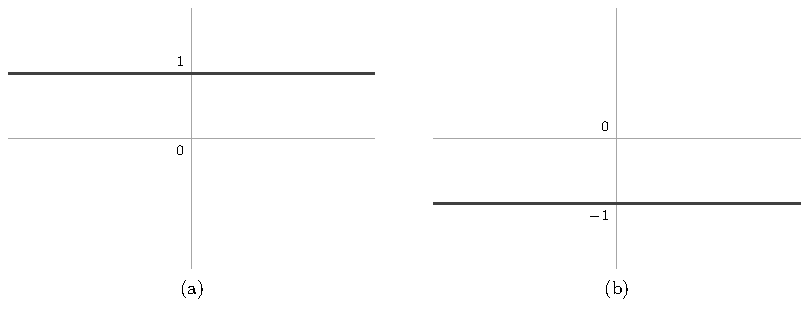
\includegraphics{figuras/funcion-constante.pdf}
        \caption{Gráfica de la función constante $f(x)=c$ en los casos en que $c=1$ y $c=-1$,
        respectivamente.}
    \end{figure}

    \begin{figure}[H]
        \centering
        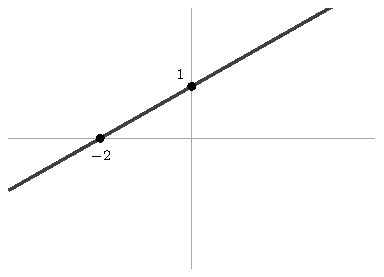
\includegraphics{figuras/recta.pdf}
        \caption{Gráfica de la función $f(x)=mx+b$ (con $m=1/2$ y $b=1$). En este caso la
        gráfica de la función $f$ es una recta de pendiente $m$ y cuya intersección con el eje $Y$ es el
        punto $(0,b)$.}
    \end{figure}

    \begin{figure}[H]
        \centering
        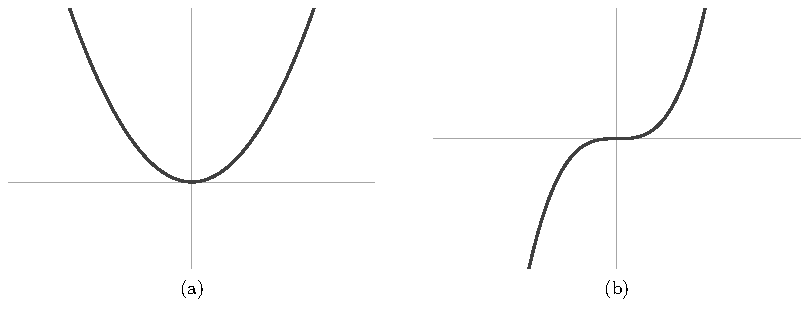
\includegraphics{figuras/potencias.pdf}
        \caption{Gráfica de la función $f(x)=x^{n}$ ($n=2,3$, respectivamente).}
    \end{figure}

    \begin{figure}[H]
        \centering
        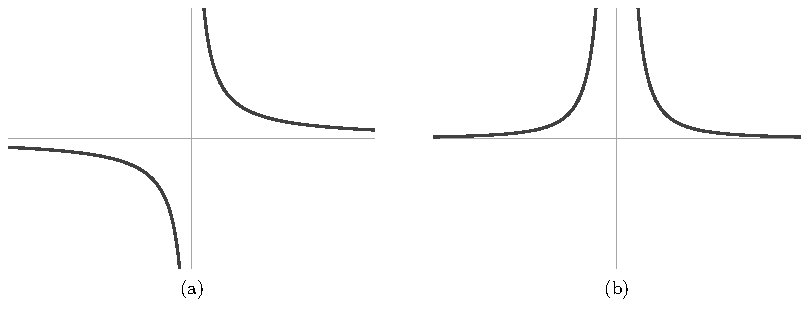
\includegraphics{figuras/reciprocos.pdf}
        \caption{Gráfica de la función $f(x)=1/x^{n}$ ($n=1,2$, respectivamente).}
    \end{figure}

    \begin{figure}[H]
        \centering
        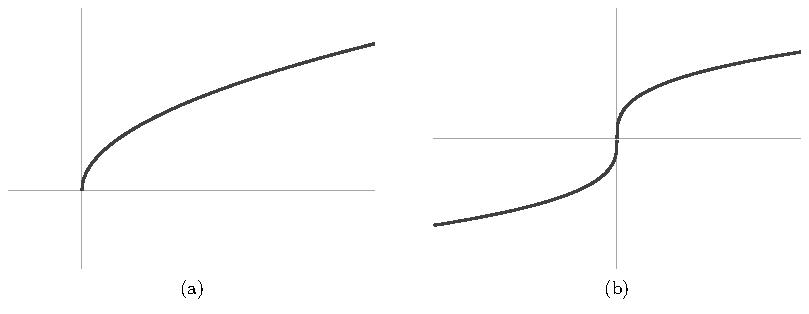
\includegraphics{figuras/raices.pdf}
        \caption{Gráfica de la función raíz $n$-ésima $\sqrt[n]{x}$ ($n=2,3$, respectivamente).}
    \end{figure}

    \begin{figure}[H]
        \centering
        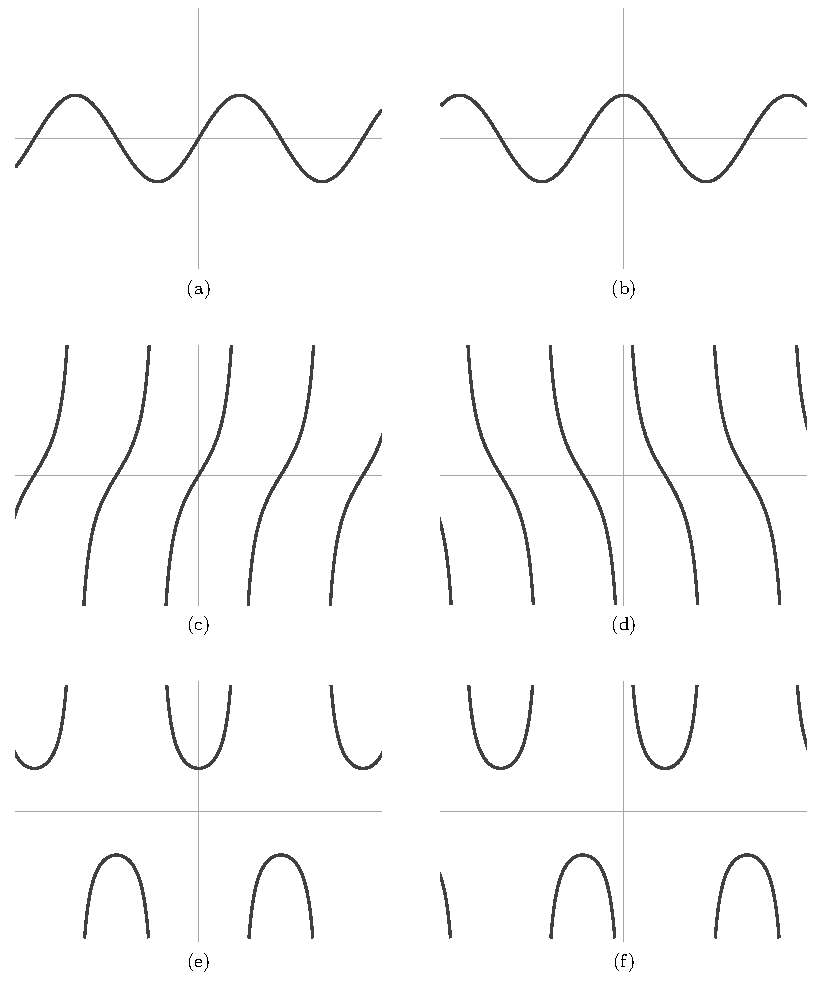
\includegraphics{figuras/trigonometricas.pdf}
        \caption{Gráfica de las funciones trigonométricas: seno, coseno, tangente, cotangente,
        secante y cosecante, respectivamente.}
    \end{figure}

    \begin{figure}[H]
        \centering
        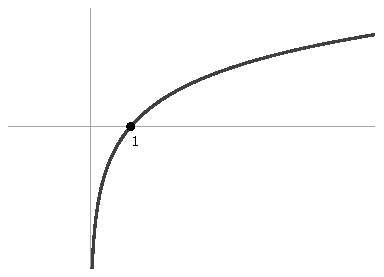
\includegraphics{figuras/logaritmo.pdf}
        \caption{Gráfica de la función logaritmo natural $\ln(x)$.}
    \end{figure}

    \begin{figure}[H]
        \centering
        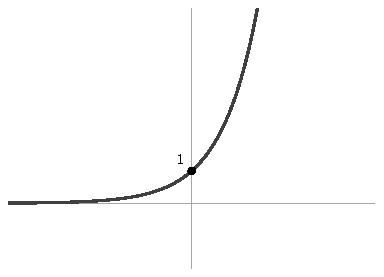
\includegraphics{figuras/exponencial.pdf}
        \caption{Gráfica de la función exponencial $e^{x}$.}
    \end{figure}

    \begin{figure}[H]
        \centering
        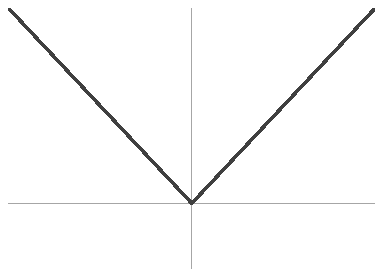
\includegraphics{figuras/valor-absoluto.pdf}
        \caption{Gráfica de la función valor absoluto $|x|$}
        \label{fig:3.10}
    \end{figure}

    \textbf{Gráfica de otras funciones:}

    \begin{figure}[H]
        \centering
        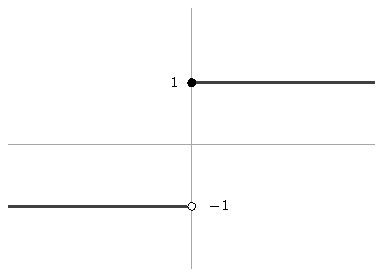
\includegraphics{figuras/escalon.pdf}
        \caption{Gráfica de la función $f(x)=\begin{cases}1, & \text{si }x\geq 0\\ -1, & \text{si }x<0.\end{cases}$}
    \end{figure}

    \begin{figure}[H]
        \centering
        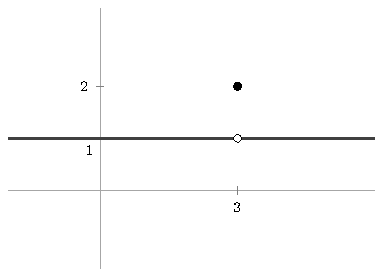
\includegraphics{figuras/funcion-salto-punto.pdf}
        \caption{Gráfica de la función $f(x)=\begin{cases}1, & \text{si }x\neq 3\\ 2, & \text{si }x=3.\end{cases}$}
        \label{fig:3.12}
    \end{figure}

    \begin{figure}[H]
        \centering
        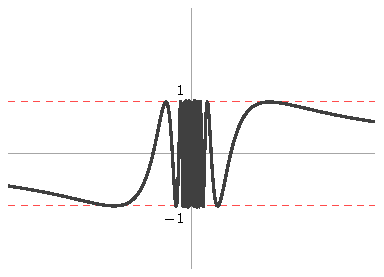
\includegraphics{figuras/seno-uno-entre-x.pdf}
        \caption{Gráfica de la función $f(x)=\begin{cases}\sin(1/x), & \text{si }x\neq 0,\\ 0, & \text{si }x=0.\end{cases}$}
        \label{fig:3.13}
    \end{figure}

    \begin{figure}[H]
        \centering
        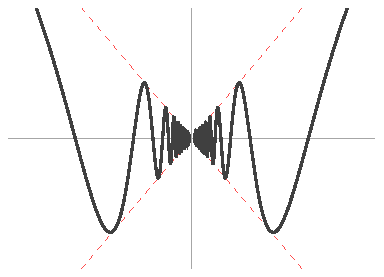
\includegraphics{figuras/x-seno-uno-entre-x.pdf}
        \caption{Gráfica de la función $f(x)=\begin{cases}x\sin(1/x), & \text{si }x\neq 0,\\ 0, & \text{si }x=0.\end{cases}$}
        \label{fig:3.14}
    \end{figure}

    \begin{figure}[H]
        \centering
        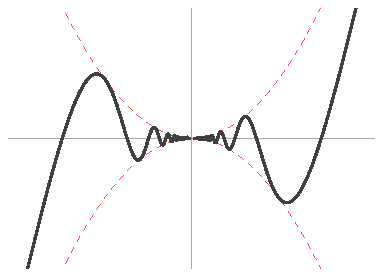
\includegraphics{figuras/x2-seno-uno-entre-x.pdf}
        \caption{Gráfica de la función $f(x)=\begin{cases}x^{2}\sin(1/x), & \text{si }x\neq 0,\\ 0, & \text{si }x=0.\end{cases}$}
        \label{fig:3.15}
    \end{figure}

    La gráfica de una función es por definición un subconjunto del plano cartesiano,
    surge la pregunta siguiente, ¿todo subconjunto del plano es la gráfica
    de una función? La respuesta es que no. El criterio siguiente, el cual se deduce
    de la definición de función, nos ayudará a determinar si un subconjunto del
    plano es la gráfica de una función.

    \begin{proposicion}[Criterio de la recta vertical para determinar si un subconjunto del plano es la gráfica de una función]\label{prop:22}
        \index{criterio de la recta vertical para determinar si una curva en el plano es la grafica de una funcion@criterio de la recta vertical para determinar si una curva en el plano es la gráfica de una función}Sea $G$ un subconjunto
        del plano. Entonces $G$ es la gráfica de cierta función si y solo si toda
        recta vertical intersecta a $G$ a lo más en un punto.
    \end{proposicion}

    \begin{ejemplo}\label{ejm:21}
        Consideremos la curva $\alpha$ de la figura~\ref{fig:3.16}, es decir, $\alpha$ es la
        circunferencia con centro en el origen y radio $1$. ¿Es $\alpha$ la gráfica de alguna
        función $f$? La respuesta es que no, pues, por ejemplo, la recta $x=0$ intersecta
        a $\alpha$ en más de un punto, a saber, en los puntos $(0,1)$ y $(0,-1)$.
    \end{ejemplo}

    \begin{ejemplo}\label{ejm:22}
        Consideremos ahora la curva $\beta$ de la figura~\ref{fig:3.17}. ¿Es $\beta$ la gráfica
        de alguna función $f$? La respuesta es que no, pues, por ejemplo, la recta $x=1$
        intersecta a $\beta$ en dos puntos.
    \end{ejemplo}

    \begin{figure}[H]
        \centering
        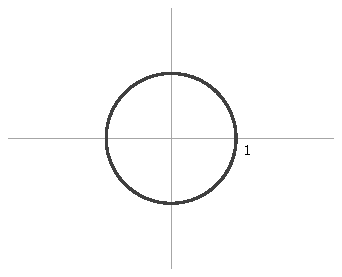
\includegraphics{figuras/circunferencia.pdf}
        \caption{La curva $\alpha$ no es la gráfica de una función.}
        \label{fig:3.16}
    \end{figure}

    \begin{figure}[H]
        \centering
        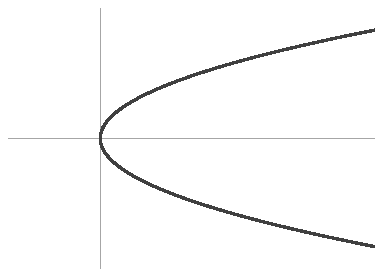
\includegraphics{figuras/parabola-horizontal.pdf}
        \caption{La curva $\beta$ no es la gráfica de una función.}
        \label{fig:3.17}
    \end{figure}

    \begin{ejemplo}\label{ejm:23}
        Como otro ejemplo, consideremos la curva $\gamma$ de la figura~\ref{fig:3.18}.
        ¿Es $\gamma$ la gráfica de alguna función $f$? La respuesta es que no, pues, por
        ejemplo, la recta $x=0$ intersecta a $\gamma$ en más de un punto.
    \end{ejemplo}

    \begin{figure}[H]
        \centering
        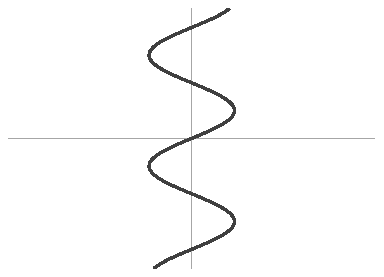
\includegraphics{figuras/curva-gamma.pdf}
        \caption{La curva $\gamma$ no es la gráfica de una función.}
        \label{fig:3.18}
    \end{figure}

    \par\avoidorphan{6}\subsection*{Ejercicios}

    \begin{ejercicio}\label{ej:94}
        Dibuja la gráfica de la función
        \begin{equation*}
            f(x)=\begin{cases}
                -1, & \text{si }x\leq 0,\\
                x, & \text{si }x>0.
            \end{cases}
        \end{equation*}
    \end{ejercicio}

    \begin{ejercicio}\label{ej:95}
        Dibuja la gráfica de la función
        \begin{equation*}
            f(x)=\begin{cases}
                x^{2}+2, & \text{si }x\leq 1,\\
                x+1, & \text{si }x>1.
            \end{cases}
        \end{equation*}
    \end{ejercicio}

    \begin{ejercicio}\label{ej:96}
        Sea $f:\R\to\R$ definida como
        \begin{equation*}
            f(x)=x^{2}.
        \end{equation*}
        Dibuja las gráficas de $f$, $f|_{[0,\infty)}$, $f|_{(-\infty,0]}$, $f|_{[-1,1]}$, $f|_{(-1,1]}$ y $f|_{[-1,1)}$.
    \end{ejercicio}

    \begin{ejercicio}[Mínimo y máximo de dos funciones]\label{ej:97}
        \index{minimo de dos funciones@mínimo de dos funciones}\index{maximo de dos funciones@máximo de dos funciones}Dadas dos funciones
        $f$ y $g$ con el mismo dominio $A$, definimos el mínimo de $f$ y $g$ como la
        función
        \begin{equation*}
            \min\{f,g\}(x)=\min\{f(x),g(x)\},\ \ x\in A
        \end{equation*}
        y el máximo de $f$ y $g$ como la función
        \begin{equation*}
            \max\{f,g\}(x)=\max\{f(x),g(x)\},\ \ x\in A.
        \end{equation*}
        Dibuja la gráfica de las funciones $\min\{f,g\}$ y $\max\{f,g\}$ para las funciones
        siguientes:
        \begin{multicols}{2}
        \begin{enumerate}[nosep]
            \item $f(x)=x$ y $g(x)=x^{2}$.
            \item $f(x)=x^{2}$ y $g(x)=x^{3}$.
        \end{enumerate}
        \end{multicols}
    \end{ejercicio}

    \section{Funciones Pares e Impares}

    Toca el turno de estudiar a las funciones pares e impares. Geométricamente,
    una función es par si su gráfica se refleja en el eje $Y$, y una función es impar
    si su gráfica se refleja en el origen. Por ejemplo, las funciones $x^{2}$ y $\cos(x)$ son
    pares y las funciones $x^{3}$ y $\sin(x)$ son impares (véase las figuras~\ref{fig:3.19} y~\ref{fig:3.20}).
    Analíticamente la definición de función pare e impar es la siguiente.

    \begin{definicion}[Funciones pares e impares]\label{def:23}
        Sea $f$ una función.
        \begin{enumerate}
            \item Diremos que $f$ es \textit{par}\index{funcion par@función par} si
            \begin{equation*}
                f(-x)=f(x)\ \text{para todo }x\in\dom(f).
            \end{equation*}
            \item Diremos que $f$ es \textit{impar}\index{funcion impar@función impar} si
            \begin{equation*}
                f(-x)=-f(x)\ \text{para todo }x\in\dom(f).
            \end{equation*}
        \end{enumerate}
    \end{definicion}

    De manera informal podemos decir que una función par «elimina» el signo
    de la variable y que una función impar «saca» el signo de la función.

    \begin{figure}[H]
        \centering
        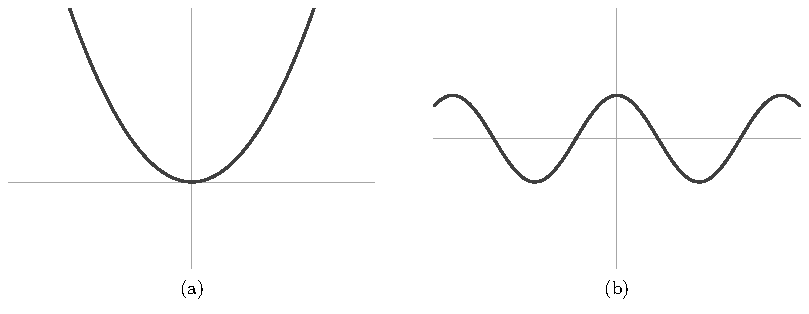
\includegraphics{figuras/paridad-pares.pdf}
        \caption{Las funciones $x^{2}$ y $\cos(x)$ son pares.}
        \label{fig:3.19}
    \end{figure}

    \begin{figure}[H]
        \centering
        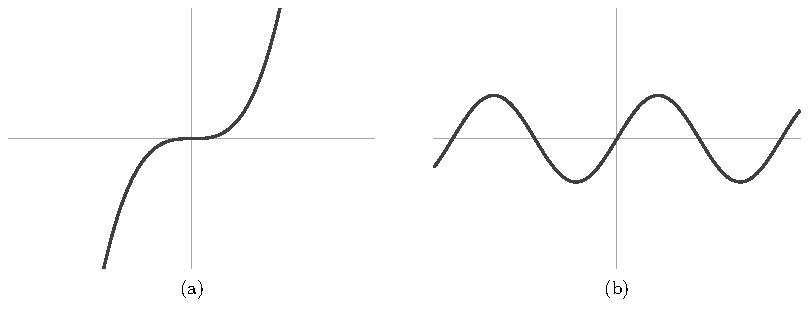
\includegraphics{figuras/paridad-impares.pdf}
        \caption{Las funciones $x^{3}$ y $\sin(x)$ son impares.}
        \label{fig:3.20}
    \end{figure}

    \begin{ejemplo}\label{ejm:24}
        La función valor absoluto $|x|$ es par, pues su gráfica se refleja
        en el eje $Y$. Por otra parte, la función $|x|$ no es impar, pues, por ejemplo,
        $|-1|\neq -|1|$.
    \end{ejemplo}

    \begin{ejemplo}\label{ejm:25}
        Como ya comentamos anteriormente, la función $x^{2}$ es par. Por
        otra parte, la función $x^{2}$ no es impar, pues, por ejemplo, $(-1)^{2}\neq -1^{2}$.
    \end{ejemplo}

    \begin{ejemplo}\label{ejm:26}
        Como ya comentamos anteriormente, la función $x^{3}$ es impar.
        Por otra parte, la función $x^{3}$ no es par, pues, por ejemplo, $(-1)^{3}\neq 1^{3}$.
    \end{ejemplo}

    \begin{ejemplo}\label{ejm:27}
        La función $f(x)=x^{3}+1$ no es par, pues, por ejemplo, $f(-1)\neq
        f(1)$. La función $f$ tampoco es impar, pues, por ejemplo, $f(-0)\neq -f(0)$.
        Recomendamos al lector dibujar la gráfica de $f$ y verificar que no es simétrica
        respecto al eje $Y$ ni respecto al origen.
    \end{ejemplo}

    ¿Existirán funciones que son tanto pares como impares? En caso afirmativo,
    ¿cuáles son? Véase el ejercicio~\ref{ej:100}.

    \par\avoidorphan{6}\subsection*{Ejercicios}

    \begin{ejercicio}\label{ej:98}
        Determina si las funciones siguientes son pares, impares o ninguna
        de las dos cosas. Argumenta tu respuesta.
        \begin{multicols}{2}
        \begin{enumerate}[nosep]
            \item $f(x)=\sqrt[3]{x}$.
            \item $f(x)=\sin^{2}(x)$.
        \end{enumerate}
        \end{multicols}
    \end{ejercicio}

    \begin{ejercicio}\label{ej:99}
        Determina si las funciones siguientes son pares, impares o ninguna
        de las dos cosas. Argumenta tu respuesta.
        \begin{multicols}{2}
        \begin{enumerate}[nosep]
            \item $f(x)=x^{2}\left(4-x^{2}\right)$.
            \item $f(x)=x\cos(x)$.
        \end{enumerate}
        \end{multicols}
    \end{ejercicio}

    \begin{ejercicio}\label{ej:100}
        ¿Existen funciones que son tanto pares como impares? En
        caso afirmativo, ¿qué forma tienen? Argumenta tu respuesta.
    \end{ejercicio}

    \begin{ejercicio}\label{ej:101}
        Prueba o da un contraejemplo a las afirmaciones siguientes:
        \begin{enumerate}[nosep]
            \item Si $f$ y $g$ son funciones pares (impares), entonces $f+g$ es par (impar).
            \item Si $f$ y $g$ son funciones pares (impares), entonces $f-g$ es par (impar).
            \item Si $f$ y $g$ son funciones pares (impares), entonces $fg$ es par (impar).
            \item Si $f$ y $g$ son funciones pares (impares), entonces $f/g$ es par (impar).
        \end{enumerate}
    \end{ejercicio}

    \begin{ejercicio}\label{ej:102}
        Sean $f$ y $g$ funciones. Estudia la paridad (par o impar) de la
        función $f\circ g$ en términos de la paridad de $f$ y $g$. Argumenta tus respuestas.
    \end{ejercicio}

    \section{Funciones Monótonas}

    En esta pequeña sección introduciremos a las funciones monótonas, una
    clase importante de funciones que estudiaremos más a fondo en las próximas
    secciones y capítulos.

    \begin{definicion}[Funciones monótonas]\label{def:24}
        Sea $f$ una función definida en un
        intervalo $I$ de números reales.
        \begin{enumerate}
            \item Diremos que $f$ es \textit{creciente}\index{funcion creciente@función creciente} en $I$ si para toda $x,y\in I$,
            \begin{equation*}
                x<y\text{ implica que }f(x)<f(y).
            \end{equation*}
            \item Diremos que $f$ es \textit{monótona creciente}\index{funcion monotona creciente@función monótona creciente} en $I$ si para toda $x,y\in I$,
            \begin{equation*}
                x<y\text{ implica que }f(x)\leq f(y).
            \end{equation*}
            \item Diremos que $f$ es \textit{decreciente}\index{funcion decreciente@función decreciente} en $I$ si para toda $x,y\in I$,
            \begin{equation*}
                x<y\text{ implica que }f(x)>f(y).
            \end{equation*}
            \item Diremos que $f$ es \textit{monótona decreciente}\index{funcion monotona decreciente@función monótona decreciente} en $I$ si para toda $x,y\in I$,
            \begin{equation*}
                x<y\text{ implica que }f(x)\geq f(y).
            \end{equation*}
            \item Diremos que $f$ es \textit{monótona}\index{funcion monotona@función monótona} en $I$ si $f$ es monótona creciente o monótona
            decreciente en $I$.
        \end{enumerate}
    \end{definicion}

    Notemos que toda función creciente (decreciente) es monótona creciente
    (decreciente), sin embargo, no se cumple el recíproco. La figura~\ref{fig:3.21} muestra
    la gráfica de algunas funciones monótonas.

    \begin{figure}[H]
        \centering
        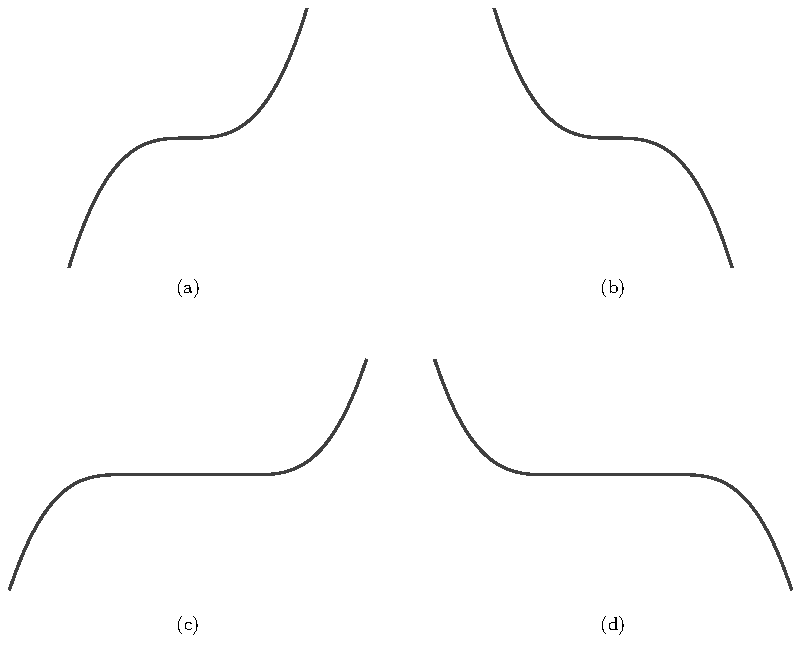
\includegraphics{figuras/monotonas.pdf}
        \caption{Gráfica de algunas funciones monótonas. La función del inciso (a) es creciente,
        la del inciso (b) es decreciente, la del inciso (c) es monótona creciente y la del inciso
        (d) es monótona decreciente.}
        \label{fig:3.21}
    \end{figure}

    Como comentamos anteriormente, en las próximas secciones y capítulos
    estudiaremos más a fondo a las funciones monótonas, una vez que tengamos
    las herramientas necesarias para ello. Por lo pronto sabemos que, por el
    ejercicio~\ref{ej:59}, la función $x^{n}$ es decreciente en el intervalo $(-\infty,0]$ y creciente
    en el intervalo $[0,\infty)$ si $n$ es un número natural par; y que es creciente en
    todo $\R$ si $n$ es impar. También sabemos, por el ejercicio~\ref{ej:60}, que la función
    $\sqrt[n]{x}$ es creciente en $[0,\infty)$ si $n$ es par y creciente en todo $\R$ si $n$ es impar.
    Más adelante, en el capítulo~\ref{cap:derivada}, mostraremos que las funciones $\ln(x)$ y $e^{x}$ son
    crecientes. Invitamos al lector a que repase la gráfica de estas funciones.

    \par\avoidorphan{6}\subsection*{Ejercicios}

    \begin{ejercicio}\label{ej:103}
        Proporciona un ejemplo de una función monótona creciente
        (monótona decreciente) que no sea creciente (decreciente).
    \end{ejercicio}

    \begin{ejercicio}\label{ej:104}
        ¿Existen funciones que son tanto crecientes como decrecientes?
        En caso afirmativo, ¿qué forma tienen? Argumenta tu respuesta.
    \end{ejercicio}

    \begin{ejercicio}\label{ej:105}
        ¿Existen funciones que son tanto monótonas crecientes como
        monótonas decrecientes? En caso afirmativo, ¿qué forma tienen? Argumenta
        tu respuesta.
    \end{ejercicio}

    \begin{ejercicio}\label{ej:106}
        Sean $f$ y $g$ funciones definidas en un intervalo $I$. Estudia la
        monotonía (creciente, decreciente, monótona creciente o monótona decreciente)
        de las funciones $f+g$, $f-g$, $fg$ y $f/g$ en términos de la monotonía de $f$
        y $g$. Argumenta tus respuestas.
    \end{ejercicio}

    \begin{ejercicio}\label{ej:107}
        Sean $I$ y $J$ intervalos, $g:I\to J$ y $f:J\to\R$. Estudia la
        monotonía (creciente, decreciente, monótona creciente o monótona decreciente)
        de la función $f\circ g$ en términos de la monotonía de $f$ y $g$. Argumenta tus
        respuestas.
    \end{ejercicio}

    \begin{ejercicio}[Desigualdades de funciones I\protect\footnote{Véase también el ejercicio~\ref{ej:207}.}]\label{ej:108}
        Sean $f$ y $g$ dos funciones
        definidas en un intervalo $[a,\infty)$ y definamos $h(x)=f(x)-g(x)$, $x\in[a,\infty)$.
        Prueba lo siguiente:
        \begin{enumerate}[nosep]
            \item Si $h$ es monótona creciente y $0\leq h(a)$, entonces $g(x)\leq f(x)$, $x\in[a,\infty)$.
            \item Si $h$ es monótona decreciente y $h(a)\leq 0$, entonces $f(x)\leq g(x)$, $x\in[a,\infty)$.
        \end{enumerate}
        Por supuesto, las desigualdades entre las funciones $f$ y $g$ de los incisos anteriores
        pueden ser estrictas en algunos casos, por ejemplo, si en el inciso (a) se
        tiene que $0<h(a)$, entonces $g(x)<f(x)$, $x\in[a,\infty)$. No enunciamos estos
        casos buscando la simplicidad en el enunciado. Resultados análogos se cumplen
        para funciones $f$ y $g$ definidas en intervalos de la forma $(-\infty,a]$, $[a,b)$
        y $(b,a]$. Este resultado, aunque sencillo, será de gran utilidad para mostrar
        desigualdades de funciones, sobre todo una vez que dispongamos de herramientas
        para determinar si una función es monótona creciente o monótona
        decreciente en la sección~\ref{sec:aplicaciones-derivada}.
    \end{ejercicio}

    \section{Transformaciones de Funciones: Traslaciones y Reflexiones}

    A partir de funciones cuya gráfica es conocida se puede construir la gráfica
    de funciones más complicadas mediante transformaciones de funciones. Las
    transformaciones básicas de funciones\index{transformaciones basicas de funciones@transformaciones básicas de funciones} se resumen en el cuadro siguiente.

    \begin{table}[H]
        \centering
        \renewcommand{\arraystretch}{1.3}
        \begin{tabular}{|c|c|p{7.2cm}|}
            \hline
            \multicolumn{3}{|c|}{\textbf{Transformaciones Básicas de Funciones}}\\
            \hline
            \textbf{Función} & \textbf{Transformación} & \multicolumn{1}{c|}{\textbf{Resultado}}\\
            \hline\noalign{\vskip 3pt}\hline
            $f(x)$ & $f(x)+c$ & La gráfica de $f$ se \textbf{traslada} $c$ unidades hacia arriba si $c>0$ o hacia abajo si $c<0$.\\ \hline
            $f(x)$ & $f(x+c)$ & La gráfica de $f$ se \textbf{traslada} $c$ unidades a la derecha si $c<0$ o hacia la izquierda si $c>0$.\\ \hline
            $f(x)$ & $-f(x)$ & La gráfica de $f$ se \textbf{refleja} en el eje $X$.\\ \hline
            $f(x)$ & $f(-x)$ & La gráfica de $f$ se \textbf{refleja} en el eje $Y$.\\ \hline
        \end{tabular}
    \end{table}

    Las seis figuras siguientes muestran el efecto de las transformaciones básicas
    sobre la gráfica de la función $\sqrt{x}$.

    \begin{figure}[H]
        \centering
        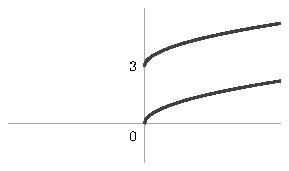
\includegraphics{figuras/raiz-mas-3.pdf}
        \caption{Gráficas de las funciones $\sqrt{x}$, $\sqrt{x}+3$}
    \end{figure}

    \begin{figure}[H]
        \centering
        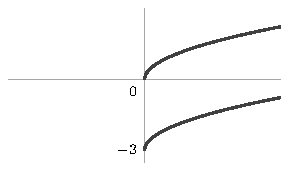
\includegraphics{figuras/raiz-menos-3.pdf}
        \caption{Gráficas de las funciones $\sqrt{x}$, $\sqrt{x}-3$}
    \end{figure}

    \begin{figure}[H]
        \centering
        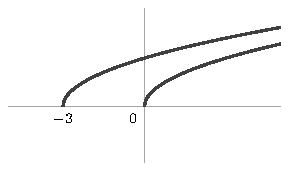
\includegraphics{figuras/raiz-x-mas-3.pdf}
        \caption{Gráficas de las funciones $\sqrt{x}$ y $\sqrt{x+3}$}
    \end{figure}

    \begin{figure}[H]
        \centering
        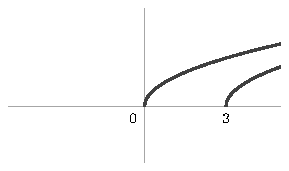
\includegraphics{figuras/raiz-x-menos-3.pdf}
        \caption{Gráficas de las funciones $\sqrt{x}$, $\sqrt{x-3}$}
    \end{figure}

    \begin{figure}[H]
        \centering
        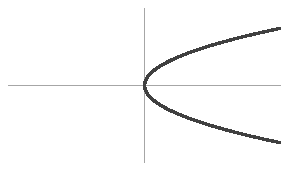
\includegraphics{figuras/raiz-reflejo-x.pdf}
        \caption{Gráficas de las funciones $\sqrt{x}$ y $-\sqrt{x}$}
    \end{figure}

    \begin{figure}[H]
        \centering
        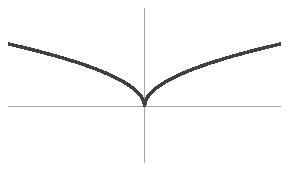
\includegraphics{figuras/raiz-reflejo-y.pdf}
        \caption{Gráficas de las funciones $\sqrt{x}$ y $\sqrt{-x}$}
    \end{figure}

    \begin{ejemplo}\label{ejm:28}
        Bosqueja la gráfica de la función $f(x)=5-\sqrt{3-x}$.

        \textbf{Solución.} Notemos que podemos obtener la función $f$, a partir de la
        función $\sqrt{x}$, mediante transformaciones básicas de funciones de la manera
        siguiente:
        \begin{equation*}
            \sqrt{x}\to\sqrt{-x}\to\sqrt{-(x-3)}=\sqrt{3-x}\to-\sqrt{3-x}\to 5-\sqrt{3-x}.
        \end{equation*}
        En consecuencia, la gráfica de $f$ es el resultado final de la secuencia de gráficas
        (de izquierda a derecha) que aparece en la figura~\ref{fig:3.28}.
    \end{ejemplo}

    \begin{figure}[H]
        \centering
        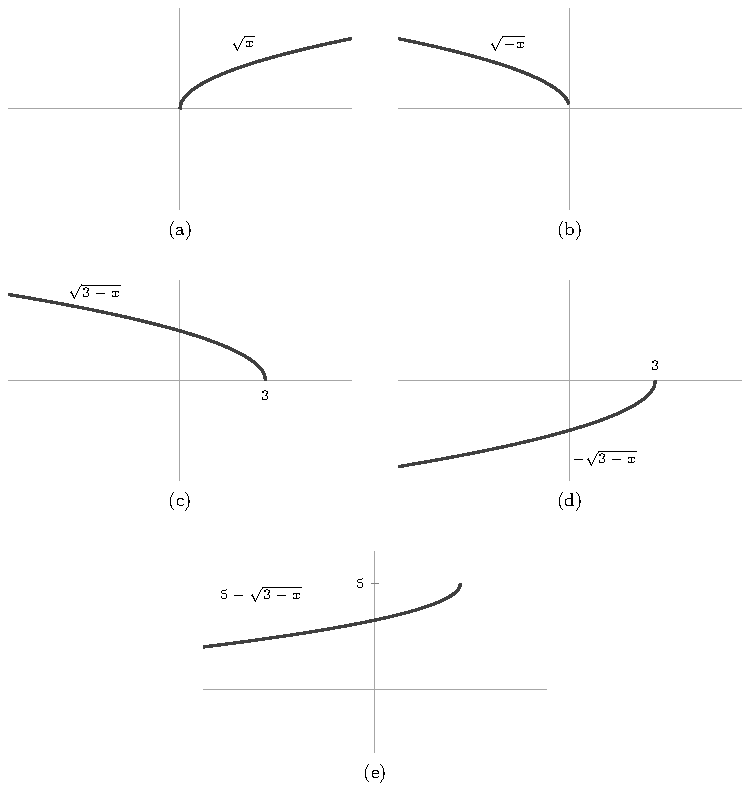
\includegraphics{figuras/transformacion-raiz.pdf}
        \caption{Secuencia de gráficas (de izquierda a derecha) que muestra la transformación
        de la función $\sqrt{x}$ en la función $f$ utilizando transformaciones básicas sobre funciones.}
        \label{fig:3.28}
    \end{figure}

    \par\avoidorphan{6}\subsection*{Ejercicios}

    \begin{ejercicio}\label{ej:109}
        ¿Qué efecto tiene la transformación $-f(-x)$ sobre la gráfica
        de una función $f$?
    \end{ejercicio}

    \begin{ejercicio}\label{ej:110}
        Utiliza la gráfica de $f(x)=\sin(x)$ para dibujar la gráfica de
        las funciones siguientes:
        \begin{multicols}{2}
        \begin{enumerate}[nosep]
            \item $y=\sin(x)+2$.
            \item $y=-\sin(x)$.
            \item $y=\sin(x-\pi/2)$.
            \item $y=\sin(-x)$.
        \end{enumerate}
        \end{multicols}
    \end{ejercicio}

    \begin{ejercicio}\label{ej:111}
        Encuentra una secuencia de transformaciones básicas sobre
        funciones que transformen a la función $\sqrt{x}$ en la función $2-\sqrt{1-x}$. Bosqueja
        la gráfica de cada una de las funciones de la secuencia.
    \end{ejercicio}

    \begin{ejercicio}\label{ej:112}
        Encuentra una secuencia de transformaciones básicas sobre
        funciones que transformen a la función $x^{2}$ en la función $-(3-x)^{2}-1$.
        Bosqueja la gráfica de cada una de las funciones de la secuencia.
    \end{ejercicio}

    \section{Cálculo del Rango de una Función}

    En ocasiones, encontrar o calcular el rango de una función $f$, es decir,
    encontrar el conjunto
    \begin{equation*}
        \{f(x):x\in\dom(f)\},
    \end{equation*}
    puede ser una tarea sencilla y algunas veces no tanto. A continuación veremos
    un artificio para encontrar el rango de una función $f$ con la propiedad de que
    de la ecuación
    \begin{equation*}
        y=f(x)
    \end{equation*}
    se puede despejar $x$ en función de $y$. Notemos que en este caso existe una
    función $g$ tal que
    \begin{equation*}
        x=g(y)
    \end{equation*}
    y, en consecuencia, el rango de $f$ está contenido en el dominio de $g$, sin
    embargo, pueden ser diferentes.

    \begin{proposicion}[Artificio para calcular el rango de una función]\label{prop:23}
        Sea $f$ una función. Si de la ecuación
        \begin{equation}\label{eq:rango-1}
            y=f(x)
        \end{equation}
        podemos despejar $x$ en función de $y$ para obtener la ecuación
        \begin{equation}\label{eq:rango-2}
            x=g(y),
        \end{equation}
        entonces
        \begin{equation}\label{eq:rango-3}
            \ran(f)=\{y\in\dom(g):f(g(y))=y\}.
        \end{equation}
    \end{proposicion}

    \begin{proof}
        Supongamos que de la ecuación \eqref{eq:rango-1} obtenemos la ecuación
        \eqref{eq:rango-2} y sea $A$ el conjunto de la derecha de \eqref{eq:rango-3}.

        ($\subset$) Tomemos $y\in\ran(f)$. Así, $y=f(x)$ para algún $x$. Luego, por \eqref{eq:rango-2},
        $x=g(y)$. En consecuencia, $y\in\dom(g)$ y $y=f(x)=f(g(y))$, lo cual
        implica que $y\in A$. Por ende, $\ran(f)\subset A$.

        ($\supset$) Sea $y\in A$. Como $f(g(y))=y$, obtenemos que $y\in\ran(f)$. Así,
        $A\subset\ran(f)$.
    \end{proof}

    Veamos algunos ejemplos.

    \begin{ejemplo}\label{ejm:29}
        Calcula el rango de la función $f(x)=2x+1$.

        \textbf{Solución.} En este ejemplo es claro que el rango de $f$ es $\R$, pues todo
        número real se puede escribir en la forma $2x+1$. Comparemos esto con el
        resultado que nos proporciona el artificio anterior: Notemos que de la ecuación
        \begin{equation*}
            y=2x+1
        \end{equation*}
        podemos despejar $x$ en función de $y$ para obtener la ecuación
        \begin{align*}
            x&=\frac{y-1}{2}\\
            &\eqqcolon g(y).
        \end{align*}
        Claramente $\dom(g)=\R$. Por otra parte,
        \begin{align*}
            f(g(y))=y&\Leftrightarrow f\left(\frac{y-1}{2}\right)=y\\
            &\Leftrightarrow y=y.
        \end{align*}
        Por lo tanto, por el artificio anterior,
        \begin{align*}
            \ran(f)&=\{y\in\dom(g):f(g(y))=y\}\\
            &=\{y\in\R:y=y\}\\
            &=\R.\finej
        \end{align*}
    \end{ejemplo}

    \begin{ejemplo}\label{ejm:30}
        Calcula el rango de la función
        \begin{equation*}
            f(x)=\frac{1}{x}+2.
        \end{equation*}

        \textbf{Solución.} Notemos que de la ecuación
        \begin{equation*}
            y=\frac{1}{x}+2
        \end{equation*}
        podemos despejar $x$ en función de $y$ para obtener la ecuación
        \begin{align*}
            x&=\frac{1}{y-2}\\
            &\eqqcolon g(y).
        \end{align*}
        Claramente $\dom(g)=\R\backslash\{2\}$. Por otra parte,
        \begin{align*}
            f(g(y))=y&\Leftrightarrow f\left(\frac{1}{y-2}\right)=y\\
            &\Leftrightarrow y=y.
        \end{align*}
        Por lo tanto,
        \begin{align*}
            \ran(f)&=\{y\in\dom(g):f(g(y))=y\}\\
            &=\{y\in\R\backslash\{2\}:y=y\}\\
            &=\R\backslash\{2\}.\finej
        \end{align*}
    \end{ejemplo}

    \begin{ejemplo}\label{ejm:31}
        Calcula el rango de la función $f(x)=\sqrt{x-7}$.

        \textbf{Solución.} Notemos que de la ecuación
        \begin{equation*}
            y=\sqrt{x-7}
        \end{equation*}
        podemos despejar $x$ en función de $y$ para obtener la ecuación
        \begin{align*}
            x&=y^{2}+7\\
            &\eqqcolon g(y)
        \end{align*}
        Claramente $\dom(g)=\R$. Por otra parte,
        \begin{align*}
            f(g(y))=y&\Leftrightarrow f\left(y^{2}+7\right)=y\\
            &\Leftrightarrow\sqrt{y^{2}}=y\\
            &\Leftrightarrow|y|=y.
        \end{align*}
        Por lo tanto,
        \begin{align*}
            \ran(f)&=\{y\in\dom(g):f(g(y))=y\}\\
            &=\{y\in\R:|y|=y\}\\
            &=[0,\infty).\finej
        \end{align*}
    \end{ejemplo}

    Desafortunadamente no siempre podemos usar el artificio de la proposición~\ref{prop:23},
    por ejemplo, si $f(x)=\sin(x)$, no podemos despejar $x$ en función de $y$
    en la ecuación $y=\sin(x)$. En estos casos, el criterio geométrico siguiente,
    el cual se deduce de la definición del rango de una función, nos ayudará a
    encontrar el rango de $f$ si conocemos con exactitud su gráfica.

    \begin{proposicion}[Criterio de la recta horizontal para encontrar valores en el rango de una función]\label{prop:24}
        \index{criterio de la recta horizontal para encontrar valores en el rango de una funcion@criterio de la recta horizontal para encontrar valores en el rango de una función}Sea $f$ una función. Entonces $c\in
        \ran(f)$ si y solo si la recta horizontal $y=c$ intersecta a la gráfica de $f$.
    \end{proposicion}

    \begin{ejemplo}\label{ejm:32}
        Según la gráfica de la función $f(x)=x^{2}$, toda recta de la forma
        $y=c$ con $c\geq 0$ intersecta a la gráfica de $f$ y toda recta de la forma $y=c$
        con $c<0$ no la intersecta. Así, $\ran(f)=[0,\infty)$.
    \end{ejemplo}

    \begin{ejemplo}\label{ejm:33}
        Según la gráfica de la función $f(x)=x^{3}$, toda recta de la forma
        $y=c$ con $c\in\R$ intersecta a la gráfica de $f$. Así, $\ran(f)=\R$.
    \end{ejemplo}

    \begin{ejemplo}\label{ejm:34}
        Según la gráfica de la función $f(x)=\sqrt{x}$, toda recta de la
        forma $y=c$ con $c\geq 0$ intersecta a la gráfica de $f$ y toda recta de la forma
        $y=c$ con $c<0$ no la intersecta. Así, $\ran(f)=[0,\infty)$.
    \end{ejemplo}

    \begin{ejemplo}\label{ejm:35}
        Según la gráfica de la función $f(x)=\sin(x)$, toda recta de la
        forma $y=c$ con $-1\leq c\leq 1$ intersecta a la gráfica de $f$ y toda recta de la
        forma $y=c$ con $c<-1$ o $c>1$ no la intersecta. Así, $\ran(f)=[-1,1]$, como
        ya habíamos dicho en el cuadro~\ref{tab:3.1}.
    \end{ejemplo}

    \begin{ejemplo}\label{ejm:36}
        Según la gráfica de la función $f(x)=1/x$, toda recta de la
        forma $y=c$ con $c\neq 0$ intersecta a la gráfica de $f$ y la recta $y=0$ no la
        intersecta. Así, $\ran(f)=\R\backslash\{0\}$.
    \end{ejemplo}

    \begin{ejemplo}\label{ejm:37}
        Según la gráfica de la función $f(x)=1/\left(1+x^{2}\right)$, toda recta
        de la forma $y=c$ con $0<c\leq 1$ intersecta a la gráfica de $f$ y toda recta de
        la forma $y=c$ con $c\leq 0$ o $c>1$ no la intersecta. Así, $\ran(f)=(0,1]$.
    \end{ejemplo}

    \textbf{¡Peligro!} Si no se conoce con exactitud la gráfica de una función $f$
    corremos el peligro de aplicar incorrectamente el criterio de la recta horizontal
    para encontrar valores en su rango, lo cual conducirá a un cálculo incorrecto
    de $\ran(f)$. Por ejemplo, aparentemente toda recta de la forma $y=c$ con
    $c\in\R$ intersecta a la gráfica de la función
    \begin{equation}\label{eq:f-racional-irracional}
        f(x)=\begin{cases}
            x, & \text{si }x\in\Q,\\
            0, & \text{si }x\in\I,
        \end{cases}
    \end{equation}
    (véase la figura~\ref{fig:3.29}) y, en consecuencia, pensaríamos de manera incorrecta
    que $\ran(f)$ es $\R$. Sin embargo, las rectas de la forma $y=c$ con $c\in\I$ no
    intersectan a la gráfica de $f$ y solo las rectas de la forma $y=c$ con $c\in\Q$ la
    intersectan. Así, el rango de $f$ es $\Q$ y no $\R$.

    \begin{figure}[H]
        \centering
        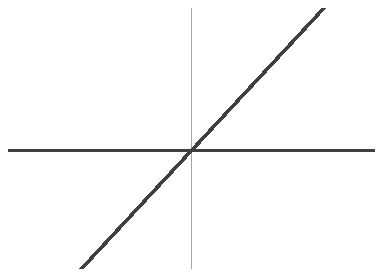
\includegraphics{figuras/racionales-irracionales.pdf}
        \caption{Gráfica de la función $f(x)=\begin{cases}x, & \text{si }x\in\Q,\\ 0, & \text{si }x\in\I.\end{cases}$ Aparentemente la gráfica de
        esta función consiste en dos rectas, la recta $y=x$ y la recta $y=0$, sin embargo, esto
        contradice el criterio de la recta vertical para determinar si una curva en el plano es la
        gráfica de una función, ¿qué está pasando entonces?}
        \label{fig:3.29}
    \end{figure}

    \par\avoidorphan{6}\subsection*{Ejercicios}

    \begin{ejercicio}\label{ej:113}
        Calcula el rango de las funciones siguientes utilizando su gráfica
        y la proposición~\ref{prop:24}.
        \begin{multicols}{2}
        \begin{enumerate}[nosep]
            \item $f(x)=x^{2}-5$.
            \item $g(x)=x^{3}+2x+7$.
            \item $h(x)=\frac{2}{x-3}$.
            \item $i(x)=\sin(x)+2$.
            \item $j(x)=\begin{cases}-1, & \text{si }x\leq 0,\\ 1, & \text{si }x>0.\end{cases}$
            \item $k(x)=\begin{cases}x, & \text{si }x\leq 3,\\ x+1, & \text{si }x>3.\end{cases}$
            \item $l(x)=\begin{cases}x^{2}, & \text{si }x\neq 2,\\ 5, & \text{si }x=2.\end{cases}$
        \end{enumerate}
        \end{multicols}
    \end{ejercicio}

    \section{Funciones Inyectivas, Suprayectivas y Biyectivas; Funciones Invertibles}\label{sec:inyectivas}

    En esta sección introduciremos a las funciones inyectivas, suprayectivas y
    biyectivas, las cuales nos permitirán estudiar con mayor profundidad a las
    funciones. Además de lo anterior, introduciremos a las funciones invertibles,
    funciones de suma importancia en el cálculo y en matemáticas.

    \begin{definicion}[Funciones inyectivas, suprayectivas y biyectivas]\label{def:25}
        Sea $f:A\to B$.
        \begin{enumerate}
            \item Diremos que $f$ es \textit{inyectiva}\index{funcion inyectiva@función inyectiva} o \textit{1-1}\index{funcion 1-1@función 1-1} si para todo $x,y\in A$ se cumple que
            \begin{equation*}
                x\neq y\text{ implica que }f(x)\neq f(y).
            \end{equation*}
            \item Diremos que $f$ es \textit{suprayectiva}\index{funcion suprayectiva@función suprayectiva} o \textit{sobre}\index{funcion sobre@función sobre} si $\ran(f)=B$, es decir, si para
            cada $y\in B$, existe $x\in A$ tal que $f(x)=y$.
            \item Diremos que $f$ es \textit{biyectiva}\index{funcion biyectiva@función biyectiva} si $f$ es inyectiva y suprayectiva. En este caso
            diremos que $f$ es una biyección entre los conjuntos $A$ y $B$.
        \end{enumerate}
    \end{definicion}

    Según su definición, una función 1-1 es la que manda puntos distintos en
    su dominio a puntos distintos en su rango, esto conduce al criterio geométrico
    siguiente para determinar si una función es 1-1.

    \begin{proposicion}[Criterio de la recta horizontal para determinar si una función es 1-1]\label{prop:25}
        \index{criterio de la recta horizontal para determinar si una funcion es 1-1@criterio de la recta horizontal para determinar si una función es 1-1}Una función $f$ es 1-1 si toda recta horizontal corta a
        la gráfica de $f$ a lo más en un punto.
    \end{proposicion}

    Así, por ejemplo, según sus gráficas, las funciones $x^{n}$ con $n$ impar, $\sqrt[n]{x}$,
    $e^{x}$ y $\ln(x)$ son funciones 1-1. Por otra parte, las funciones $x^{n}$ con $n$ par, $|x|$,
    $\sin(x)$, $\cos(x)$ y $\tan(x)$ son ejemplos de funciones que no son 1-1.

    Si no conocemos la gráfica de una función $f$ no podemos utilizar el criterio
    de la proposición~\ref{prop:25}. En este caso, la herramienta que tenemos hasta este
    momento para determinar si $f$ es 1-1 es la definición~\ref{def:25}, sin embargo, el
    verificar que una función es 1-1 usando la definición~\ref{def:25} puede, algunas veces,
    no ser sencillo. En estos casos la proposición siguiente, cuya demostración se
    deja a cargo del lector (véase el ejercicio~\ref{ej:115}), será de utilidad.

    \begin{proposicion}\label{prop:26}
        Sea $f$ una función. Son equivalentes:
        \begin{enumerate}[nosep]
            \item La función $f$ es 1-1.
            \item Para todo $x,y\in\dom(f)$ se cumple que
            \begin{equation*}
                f(x)=f(y)\text{ implica que }x=y.
            \end{equation*}
        \end{enumerate}
    \end{proposicion}

    \begin{ejemplo}\label{ejm:38}
        Determina si la función
        \begin{equation*}
            f(x)=\frac{2(x-1)^{3}}{5}+7
        \end{equation*}
        es una función 1-1.

        \textbf{Solución.} Puesto que
        \begin{align*}
            &f(x)=f(y)\\
            \Rightarrow{}& \frac{2(x-1)^{3}}{5}+7=\frac{2(y-1)^{3}}{5}+7\\
            \Rightarrow{}& (x-1)^{3}=(y-1)^{3}\\
            \Rightarrow{}& x-1=y-1 &&\text{(pues la función $x^{3}$ es 1-1)}\\
            \Rightarrow{}& x=y,
        \end{align*}
        por la proposición~\ref{prop:26} obtenemos que $f$ es 1-1.
    \end{ejemplo}

    \begin{ejemplo}\label{ejm:39}
        Determina si la función
        \begin{equation*}
            f(x)=\frac{2(x-1)^{2}}{5}+7
        \end{equation*}
        es una función 1-1.

        \textbf{Solución.} Notemos que
        \begin{align*}
            &f(x)=f(y)\\
            \Rightarrow{}& \frac{2(x-1)^{2}}{5}+7=\frac{2(y-1)^{2}}{5}+7\\
            \Rightarrow{}& (x-1)^{2}=(y-1)^{2}.
        \end{align*}
        A partir de la última ecuación no podemos asegurar que $x-1=y-1$, pues
        la función $x^{2}$ no es 1-1. De hecho, la función $f$ no es 1-1, pues, por ejemplo,
        $0\neq 2$ y $f(0)=f(2)$.
    \end{ejemplo}

    Notemos que podemos restringir el dominio de una función que no es 1-1
    de manera que la función resultante lo sea. Por ejemplo, consideremos a la
    función $f:\R\to\R$ dada por $f(x)=x^{2}+1$. Claramente la función $f$ no es
    1-1, sin embargo, si restringimos la función $f$, por ejemplo, al conjunto $[0,\infty)$
    la función resultante si lo será, es decir, la función $f|_{[0,\infty)}:[0,\infty)\to\R$ si es
    1-1 (véase la figura~\ref{fig:3.30}).

    \begin{figure}[H]
        \centering
        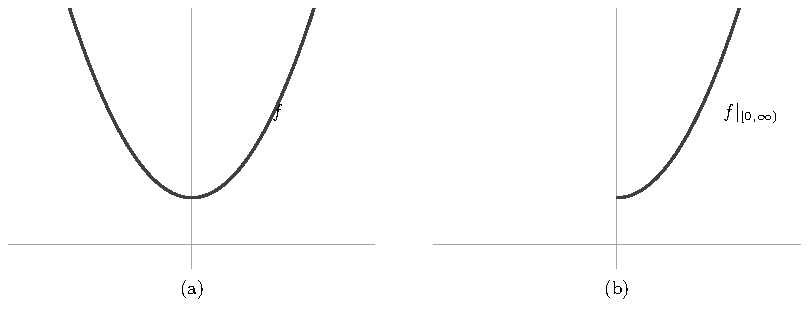
\includegraphics{figuras/restriccion-parabola.pdf}
        \caption{La función $f:\R\to\R$ dada por $f(x)=x^{2}+1$ no es 1-1, sin embargo, su
        restricción $f|_{[0,\infty)}:[0,\infty)\to\R$ si lo es.}
        \label{fig:3.30}
    \end{figure}

    Así como podemos restringir el dominio de una función para obtener funciones
    1-1, podemos restringir el codominio de una función para obtener
    una función sobre. Notemos que si restringimos el codominio de una función
    $f:A\to B$ a su rango, entonces la nueva función será sobre, es decir,
    abusando un poco de la notación,
    \begin{equation*}
        f:A\to\ran(f)
    \end{equation*}
    es una función sobre. Resumimos esta observación en la frase siguiente:
    \begin{center}
        «Toda función es sobre su rango».
    \end{center}
    Por ejemplo, la función $f:[0,\infty)\to\R$ dada por $f(x)=\sqrt{x}+1$ no es
    sobre, pues $\ran(f)=[1,\infty)\neq\R=\cod(f)$. Sin embargo, si suponemos que
    $f:[0,\infty)\to[1,\infty)$, entonces $f$ sí es sobre.

    Introducimos ahora a las funciones invertibles y sus inversas.

    \begin{definicion}[Función invertible]\label{def:26}
        Sea $f:A\to B$. Diremos que $f$ es
        \textit{invertible}\index{funcion invertible@función invertible} si existe $g:B\to A$ tal que
        \begin{equation*}
            g(f(x))=x\text{ para todo }x\in A
        \end{equation*}
        y
        \begin{equation*}
            f(g(y))=y\text{ para todo }y\in B.
        \end{equation*}
        En este caso diremos que $g$ es la \textit{inversa}\index{funcion inversa@función inversa} de $f$ y escribiremos $g=f^{-1}$.
    \end{definicion}

    Como indica la definición anterior, si existe, la inversa de una función es
    única (véase el ejercicio~\ref{ej:122}). Notemos que si $f$ es invertible, entonces
    \begin{equation}\label{eq:inversa-dom}
        \dom\left(f^{-1}\right)=\cod(f)\ \text{ y }\ \cod\left(f^{-1}\right)=\dom(f).
    \end{equation}
    Además,
    \begin{equation}\label{eq:inversa-1}
        f^{-1}(f(x))=x,\ \text{para todo }x\in\dom(f)
    \end{equation}
    y
    \begin{equation}\label{eq:inversa-2}
        f\left(f^{-1}(y)\right)=y,\ \text{para todo }y\in\cod(f).
    \end{equation}
    A partir de \eqref{eq:inversa-1} y \eqref{eq:inversa-2}, podemos decir, en palabras comunes, que $f^{-1}$
    deshace lo que $f$ hace y viceversa. Notemos también que
    \begin{equation*}
        \left(f^{-1}\right)^{-1}=f.
    \end{equation*}

    Como un primer ejemplo de una función invertible consideremos a las
    funciones $f,g:\R\to\R$ dadas por $f(x)=x^{3}$ y $g(x)=\sqrt[3]{x}$. Puesto que
    \begin{equation*}
        g(f(x))=\sqrt[3]{x^{3}}=x,\ \ x\in\R,
    \end{equation*}
    y
    \begin{equation*}
        f(g(x))=\left(\sqrt[3]{x}\right)^{3}=x,\ \ x\in\R,
    \end{equation*}
    entonces la función $g$ es la inversa de $f$.

    Para asegurar que una función es invertible disponemos del resultado
    siguiente.

    \begin{proposicion}\label{prop:27}
        Sea $f:A\to B$. La función $f$ es invertible ssi $f$ es 1-1 y
        sobre.
    \end{proposicion}

    \begin{proof}
        ($\Rightarrow$) Sea $g$ la inversa de $f$. Puesto que
        \begin{align*}
            &f(x)=f(y)\\
            \Rightarrow{}& g(f(x))=g(f(y))\\
            \Rightarrow{}& x=y,
        \end{align*}
        entonces, por la proposición~\ref{prop:26}, obtenemos que $f$ es 1-1. Resta probar que
        $f$ es sobre, es decir, que $\ran(f)=B$. Sabemos que $\ran(f)\subset B$. Tomemos
        $y\in B$. Como $g$ es la inversa de $f$, entonces
        \begin{equation*}
            y=f(g(y))\in\ran(f),
        \end{equation*}
        y, en consecuencia, $B\subset\ran(f)$. Por lo tanto, $\ran(f)=B$.

        ($\Leftarrow$) Puesto que $f$ es sobre, para cada $y\in B$, el conjunto
        \begin{equation*}
            C_{y}=\{x:f(x)=y\}
        \end{equation*}
        es no vacío. Además, como $f$ es 1-1, el conjunto $C_{y}$ consta de un solo elemento,
        digamos $x_{y}$. Definamos $g:B\to A$ como
        \begin{equation*}
            g(y)=x_{y}.
        \end{equation*}
        Es sencillo ver que $g$ es la inversa de $f$.
    \end{proof}

    En \cite{nunez2020calculoII} se prueba que la función $\ln:(0,\infty)\to\R$ es 1-1 y sobre, luego, por la
    proposición~\ref{prop:27}, la función $\ln:(0,\infty)\to\R$ es invertible. Se define la función
    exponencial $e^{x}$ como la función inversa de la función logaritmo natural $\ln(x)$.

    \textbf{Convención Importante:} De aquí en adelante, a menos que se indique
    lo contrario, cuando $f$ sea una función 1-1 en su dominio y hablemos de su
    inversa, estaremos suponiendo que su codominio es su rango (en consecuencia,
    $f$ será sobre y por la proposición~\ref{prop:27}, $f$ será invertible). Por ejemplo, la función
    $f(x)=\sqrt{x}+1$ es 1-1; su inversa es la función $g:[1,\infty)\to[0,\infty)$ dada por
    $g(x)=(x-1)^{2}$.

    Ahora veremos como obtener la gráfica de la función $f^{-1}$ a partir de la
    gráfica de $f$.

    Si $f$ es una función invertible y $y\in\ran(f)$, sabemos que existe un único
    $x\in\dom(f)$ tal que $y=f(x)$. En consecuencia,
    \begin{equation}\label{eq:grafica-inversa}
        \left(y,f^{-1}(y)\right)=(f(x),x).
    \end{equation}
    De \eqref{eq:grafica-inversa} obtenemos el criterio siguiente para encontrar la gráfica de una
    función inversa.

    \begin{proposicion}[Criterio para encontrar la gráfica de una función inversa]\label{prop:28}
        \index{criterio para encontrar la grafica de una funcion inversa@criterio para encontrar la gráfica de una función inversa}Si $f$ es una función invertible, entonces la gráfica de $f^{-1}$ se obtiene
        al reflejar la gráfica de $f$ en la recta $y=x$.
    \end{proposicion}

    La figura~\ref{fig:3.31} muestra las gráficas de las funciones $x^{3}$ y $\ln(x)$ y sus inversas
    $\sqrt[3]{x}$ y $e^{x}$, respectivamente.

    \begin{figure}[H]
        \centering
        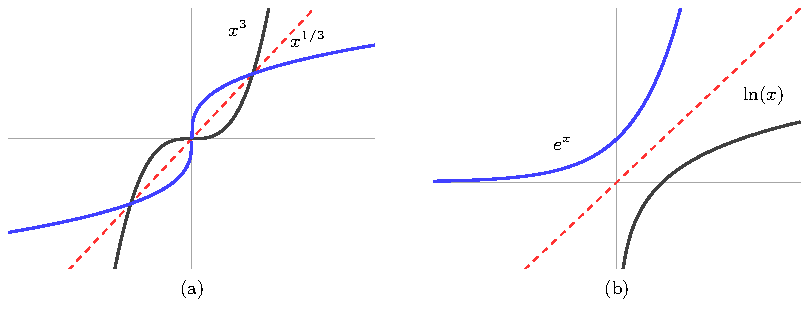
\includegraphics{figuras/inversas.pdf}
        \caption{(a) La función $x^{3}$ y su inversa $\sqrt[3]{x}$. (b) La función $\ln(x)$ y su inversa $e^{x}$.}
        \label{fig:3.31}
    \end{figure}

    La proposición siguiente, cuya prueba dejamos al lector (véase el ejercicio~\ref{ej:128}),
    señala una propiedad básica de las funciones inversas.

    \begin{proposicion}[Inversa de la composición]\label{prop:29}
        Sean $f$ y $g$ funciones
        invertibles. Si está definida la composición $f\circ g$, entonces $f\circ g$ es invertible
        y
        \begin{equation}\label{eq:inversa-composicion}
            (f\circ g)^{-1}=g^{-1}\circ f^{-1}.
        \end{equation}
    \end{proposicion}

    Para recordar la fórmula anterior, hagamos la analogía siguiente. Pensemos
    que $g$ es el proceso de ponerse los calcetines y que $f$ es el proceso de ponerse los
    zapatos. Así, podemos pensar que $f\circ g$ es el proceso de ponerse los calcetines
    y luego los zapatos, y que $(f\circ g)^{-1}$ es el proceso inverso. Con esta analogía,
    la fórmula \eqref{eq:inversa-composicion} expresa que el proceso inverso de ponerse los calcetines y
    luego los zapatos es quitarse los zapatos y luego los calcetines.

    \par\avoidorphan{6}\subsection*{Ejercicios}

    \begin{ejercicio}\label{ej:114}
        Determina si las funciones siguientes son 1-1 o sobre (recuerda
        que si no se especifica el codominio de una función, se supone, por sencillez,
        que su codominio es todo $\R$).
        \begin{multicols}{2}
        \begin{enumerate}[nosep]
            \item $f(x)=x^{2}+1$.
            \item $g(x)=\sqrt{x+1}+1$.
            \item $h(x)=2x^{3}+x$.
        \end{enumerate}
        \end{multicols}
    \end{ejercicio}

    \begin{ejercicio}\label{ej:115}
        Prueba la proposición~\ref{prop:26}.
    \end{ejercicio}

    \begin{ejercicio}\label{ej:116}
        Sea $f$ una función. Prueba que $f$ es 1-1 ssi $f(A\cap B)=
        f(A)\cap f(B)$ para todo $A,B\subset\dom(f)$.
    \end{ejercicio}

    \begin{ejercicio}\label{ej:117}
        Sean $f,g:A\to B$. Prueba o da un contraejemplo a las
        afirmaciones siguientes:
        \begin{enumerate}[nosep]
            \item Si $f$ y $g$ son 1-1, entonces $f+g$ es 1-1.
            \item Si $f$ y $g$ son 1-1, entonces $f-g$ es 1-1.
            \item Si $f$ y $g$ son 1-1, entonces $fg$ es 1-1.
            \item Si $f$ y $g$ son 1-1, entonces $f/g$ es 1-1.
        \end{enumerate}
    \end{ejercicio}

    \begin{ejercicio}\label{ej:118}
        Sean $f,g:A\to B$. Prueba o da un contraejemplo a las
        afirmaciones siguientes:
        \begin{enumerate}[nosep]
            \item Si $f$ y $g$ son sobre, entonces $f+g$ es sobre.
            \item Si $f$ y $g$ son sobre, entonces $f-g$ es sobre.
            \item Si $f$ y $g$ son sobre, entonces $fg$ es sobre.
            \item Si $f$ y $g$ son sobre, entonces $f/g$ es sobre.
        \end{enumerate}
    \end{ejercicio}

    \begin{ejercicio}\label{ej:119}
        Sean $A$, $B$ y $C$ subconjuntos de $\R$, $g:A\to B$ y $f:B\to C$,
        de manera que $f\circ g:A\to C$. Prueba lo siguiente:
        \begin{enumerate}[nosep]
            \item Si $f$ y $g$ son 1-1, entonces $f\circ g$ es 1-1.
            \item Si $f$ y $g$ son sobre, entonces $f\circ g$ es sobre.
            \item Si $f$ y $g$ son biyectivas, entonces $f\circ g$ es biyectiva.
        \end{enumerate}
    \end{ejercicio}

    \begin{ejercicio}\label{ej:120}
        Sea $f:A\to B$. Prueba o da un contraejemplo a las
        afirmaciones siguientes:
        \begin{enumerate}[nosep]
            \item Si $f$ es impar, entonces $f$ es 1-1.
            \item Si $f$ es 1-1, entonces $f$ es impar.
        \end{enumerate}
    \end{ejercicio}

    \begin{ejercicio}\label{ej:121}
        Sea $f$ una función definida en un intervalo $I$. Prueba lo
        siguiente:
        \begin{enumerate}[nosep]
            \item Si $f$ es creciente, entonces $f$ es 1-1.
            \item Si $f$ es decreciente, entonces $f$ es 1-1.
            \item Si $f$ es 1-1, ¿será $f$ creciente?, ¿será $f$ decreciente? Argumenta tu respuesta.
        \end{enumerate}
    \end{ejercicio}

    \begin{ejercicio}[Unicidad de la función inversa]\label{ej:122}
        Prueba que, si existe,
        la inversa de una función es única.
    \end{ejercicio}

    \begin{ejercicio}\label{ej:123}
        Sea $f:A\to B$ una función invertible. Prueba que $f$ es impar
        ssi $f^{-1}$ es impar.
    \end{ejercicio}

    \begin{ejercicio}\label{ej:124}
        Sea $f:I\to J$ una función sobre, donde $I$ y $J$ son intervalos.
        Prueba lo siguiente:
        \begin{enumerate}[nosep]
            \item Si $f$ es creciente, entonces $f$ es invertible y $f^{-1}$ es creciente.
            \item Si $f$ es decreciente, entonces $f$ es invertible y $f^{-1}$ es decreciente.
        \end{enumerate}
    \end{ejercicio}

    \begin{ejercicio}\label{ej:125}
        Por el criterio de la recta horizontal para determinar si una
        función es 1-1, es claro que las funciones $f(x)=x^{3}+1$ y $g(x)=e^{x-1}+1$
        son funciones 1-1. Encuentra las gráficas de $f^{-1}$ y $g^{-1}$ a partir de la gráficas
        de $f$ y $g$.
    \end{ejercicio}

    \begin{ejercicio}[Funciones trigonométricas inversas]\label{ej:126}
        \index{funciones trigonometricas inversas@funciones trigonométricas inversas}Por el criterio de
        la recta horizontal para determinar si una función es 1-1, es claro que las
        funciones trigonométricas no son funciones 1-1 y, en consecuencia, no son
        invertibles, sin embargo, restringiremos su dominio para que si lo sean. Las
        restricciones que se suelen utilizar se muestran en el cuadro siguiente.
        \begin{center}
            \renewcommand{\arraystretch}{1.3}
            \begin{tabular}{|c|c|c|}
                \hline
                \textbf{Función} & \textbf{Restricción} & \textbf{Rango de la restricción}\\ \hline
                $\sin(x)$ & $[-\pi/2,\pi/2]$ & $[-1,1]$\\ \hline
                $\cos(x)$ & $[0,\pi]$ & $[-1,1]$\\ \hline
                $\tan(x)$ & $(-\pi/2,\pi/2)$ & $\R$\\ \hline
                $\cot(x)$ & $(0,\pi)$ & $\R$\\ \hline
                $\sec(x)$ & $[0,\pi/2)\cup(\pi/2,\pi]$ & $(-\infty,-1]\cup[1,\infty)$\\ \hline
                $\csc(x)$ & $[-\pi/2,0)\cup(0,\pi/2]$ & $(-\infty,-1]\cup[1,\infty)$\\ \hline
            \end{tabular}
        \end{center}
        Las restricciones de las funciones trigonométricas señaladas en el cuadro
        anterior son 1-1 y sobre (su rango) y, en consecuencia, invertibles. A las funciones
        inversas de las restricciones señaladas en el cuadro anterior se les llama
        arcoseno, arcocoseno, arcotangente, arcocotangente, arcosecante y arcocosecante,
        respectivamente; y se les denota por $\arcsin(x)$, $\arccos(x)$, $\arctan(x)$,
        $\arccot(x)$, $\arcsec(x)$ y $\arccsc(x)$, respectivamente; son las llamadas \textit{funciones
        trigonométricas inversas}.
        \begin{enumerate}[nosep]
            \item Dibuja las gráficas de las restricciones del cuadro anterior.
            \item A partir de las gráficas del inciso (a) dibuja las gráficas de las funciones
            trigonométricas inversas.
        \end{enumerate}
    \end{ejercicio}

    \begin{ejercicio}\label{ej:127}
        Sea $f:\R\to\R$ dada por
        \begin{equation*}
            f(x)=x|x|+1.
        \end{equation*}
        \begin{enumerate}[nosep]
            \item Dibuja la gráfica de $f$.
            \item Determina si $f$ es 1-1 (argumenta tu respuesta).
            \item Determina si $f$ es sobre (argumenta tu respuesta).
            \item Determina si $f$ es invertible (argumenta tu respuesta).
            \item Si $f$ es invertible, dibuja la gráfica de su inversa.
            \item Si $f$ es invertible, calcula su inversa.
        \end{enumerate}
    \end{ejercicio}

    \begin{ejercicio}\label{ej:128}
        Prueba la proposición~\ref{prop:29}.
    \end{ejercicio}

    \chapter{Límites y Continuidad}\label{cap:limites}

    Es este capítulo definiremos y estudiaremos el concepto de límite de una
    función, el cual juega un papel crucial en matemáticas, en particular en el
    cálculo diferencial e integral. Por ejemplo, la continuidad de una función, la
    cual estudiaremos más adelante, se define en términos de un límite. La derivada,
    otro concepto fundamental en el cálculo, también se define a través de
    un límite. Por otra parte, el cálculo diferencial e integral es uno de los pilares
    de varias ramas o áreas de las matemáticas, además de otras ciencias como,
    por ejemplo, la física, química o economía, en consecuencia, el disponer de
    herramientas para calcular límites de funciones es un recurso imprescindible
    tanto en matemáticas como en otras áreas de la ciencia.

    \section{Límites Reales}

    Nos interesa estudiar como se comportan los valores $f(x)$ de una función $f$
    cuando $x$ se aproxima a un número $p$. Intuitivamente, el límite de una función
    $f$ cuando $x$ se aproxima a un número $p$ es el número $L$ si los valores $f(x)$
    de $f$ se aproximan a $L$ cuando $x$ está suficientemente cerca del número $p$. El
    problema con esta noción intuitiva de límite es que las frases «se aproximan»
    y «está suficientemente cerca» no tiene un significado preciso (matemático).
    Para remediar esta situación necesitamos primero una herramienta que nos
    permita medir la distancia entre dos números, la función valor absoluto será
    tal herramienta.

    \begin{definicion}[Distancia entre dos números]\label{def:27}
        Definimos la \textit{distancia
        entre dos números}\index{distancia entre dos numeros@distancia entre dos números} $x$ y $y$ como
        \begin{equation*}
            |x-y|.
        \end{equation*}
    \end{definicion}

    Notemos que $|x-y|$ realmente representa la distancia entre $x$ y $y$ cuando
    $x$ y $y$ son números enteros o racionales. Por ejemplo, si $x=-5$ y $y=2$,
    entonces $|x-y|=|-5-2|=|-7|=7$, y si dibujamos los números $-5$ y $2$
    sobre la recta numérica podemos apreciar que, efectivamente, el número de
    unidades entre $-5$ y $2$ es $7$.

    Si $|x-y|$ representa la distancia entre dos números $x$ y $y$, entonces al hacer
    $y=0$ obtenemos la interpretación geométrica siguiente de $|x|$.

    \begin{observacion}[Interpretación de $|x|$]\label{obs:7}
        El número $|x|$ representa la
        distancia del número $x$ al origen de la recta numérica.
    \end{observacion}

    Dada la interpretación de $|x|$ como la distancia de $x$ al origen de la recta
    numérica, la proposición siguiente, cuya prueba dejamos a cargo del lector
    (véase el ejercicio~\ref{ej:129}), parece natural.

    \begin{proposicion}\label{prop:30}
        Sea $r>0$. Se cumple lo siguiente:
        \begin{enumerate}[nosep]
            \item $|x|\geq 0$.
            \item $|x|=0$ si y solo si $x=0$.
            \item $|x|=r$ si y solo si $x=r$ o $x=-r$.
            \item $|x|<r$ si y solo si $-r<x<r$.\footnote{Recordemos que la notación $-r<x<r$ significa que $-r<x$ y que $x<r$, es decir, que
            $x\in(-r,r)$.}
            \item $|x|>r$ si y solo si $x<-r$ o $x>r$.
        \end{enumerate}
    \end{proposicion}

    Lo que dice el inciso (a) es simplemente que la distancia de un número $x$
    al origen nunca es negativa. El inciso (b) afirma que si la distancia de $x$ al
    origen es cero, entonces necesariamente $x$ debe de ser cero. Recíprocamente,
    si $x=0$ es claro que la distancia de $x$ al origen es cero. La interpretación del
    inciso (c) también es clara, la distancia entre $x$ y el origen es $r$ si y solo si
    $x=r$ o $x=-r$. La interpretación del inciso (d) es que el número $x$ está en
    el intervalo $(-r,r)$ si y solo si la distancia de $x$ al origen es menor que $r$. La
    interpretación de (e) también debe de ser clara.

    De los incisos (c), (d) y (e) de la proposición~\ref{prop:30} obtenemos el corolario
    siguiente.

    \begin{corolario}\label{cor:1}
        Se cumple lo siguiente:
        \begin{enumerate}[nosep]
            \item $|x|\leq r$ si y solo si $-r\leq x\leq r$.\footnote{Recordemos que la notación $-r\leq x\leq r$ significa que $-r\leq x$ y que $x\leq r$, es decir, que
            $x\in[-r,r]$.}
            \item $|x|\geq r$ si y solo si $x\leq -r$ o $x\geq r$.
        \end{enumerate}
    \end{corolario}

    Otras dos propiedades menos evidentes del valor absoluto, cuya prueba
    dejamos a cargo del lector (véase el ejercicio~\ref{ej:130}), son las siguientes.

    \begin{proposicion}\label{prop:31}
        Se cumple lo siguiente:
        \begin{enumerate}[nosep]
            \item $|x+y|\leq|x|+|y|$ \textbf{(desigualdad del triángulo)}\index{desigualdad del triangulo@desigualdad del triángulo}.
            \item $|xy|=|x||y|$.
        \end{enumerate}
    \end{proposicion}

    El nombre «desigualdad del triángulo» queda claro cuando se estudia la
    distancia entre dos puntos del plano o del espacio en un curso de cálculo
    de varias variables. El lector interesado en estos temas puede consultar, por
    ejemplo, \cite{apostol1974} o \cite{nunez2020calculoIII}.

    Una vez que contamos con el concepto de distancia entre dos números,
    estamos listos para dar la definición rigurosa de límite de una función. Tal
    definición, un poco complicada en un principio, es la que expresa de manera
    matemática la noción intuitiva de límite de una función que vimos al principio
    de esta subsección.

    \begin{definicion}[Límite de una función]\label{def:28}
        Sea $f$ una función definida en un
        intervalo abierto $I$ que contiene a $p$, excepto posiblemente en $p$. Diremos que
        el número real $L$ es el \textit{límite}\index{limite de una funcion@límite de una función} de $f$ cuando $x$ tiende a $p$, lo cual denotaremos
        por
        \begin{equation}\label{eq:4.1}
            \lim_{x\to p}f(x)=L,
        \end{equation}
        si para todo $\epsilon>0$, existe $\delta>0$ tal que para toda $x\in\R$, si $x\in I$ y
        $0<|x-p|<\delta$, entonces $|f(x)-L|<\epsilon$ (véase la figura~\ref{fig:4.1}).
    \end{definicion}

    En otras palabras, \eqref{eq:4.1} se cumple si para todo intervalo abierto $U$ con
    centro en $L$ y radio $\epsilon$,\footnote{El intervalo abierto $U$ con centro en $L$ y radio $\epsilon$ es el intervalo $(L-\epsilon,L+\epsilon)$ que aparece
    en la figura~\ref{fig:4.1} marcado en color rojo.} existe un intervalo abierto $V$ con centro en $p$ y radio
    $\delta$\footnote{El intervalo abierto $V$ con centro en $p$ y radio $\delta$ es el intervalo $(p-\delta,p+\delta)$ que aparece
    en la figura~\ref{fig:4.1} marcado en color azul.} tal que para todo $x\in\R$, si $x\in(I\cap V)\backslash\{p\}$, entonces $f(x)\in U$ (véase
    la figura~\ref{fig:4.1}).

    Diremos que $\lim_{x\to p}f(x)$ existe si existe un número real $L$ que cumple
    \eqref{eq:4.1}; por supuesto, en este caso al número $L$ lo denotaremos por
    $\lim_{x\to p}f(x)$. Finalmente, también escribiremos «$f(x)\to L$ cuando $x\to p$»
    para expresar que se cumple \eqref{eq:4.1}.

    \begin{figure}[H]
        \centering
        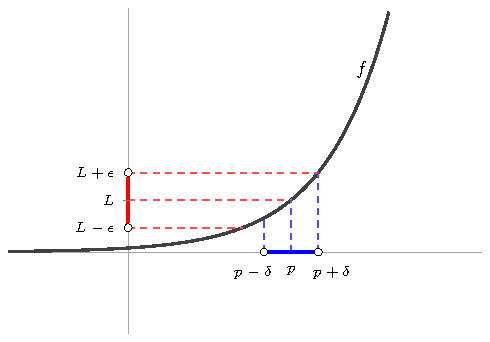
\includegraphics{figuras/limite-definicion.pdf}
        \caption{El número $L$ es el límite de la función $f$ cuando $x$ tiende a $p$.}
        \label{fig:4.1}
    \end{figure}

    \begin{observacion}\label{obs:8}
        Es importante hacer en este momento las observaciones
        siguientes:
        \begin{enumerate}[label=\arabic*.]
            \item Que $f$ esté definida en un intervalo abierto $I$ que contiene a $p$, excepto
            posiblemente en $p$, significa que $f$ está definida en el conjunto $I\backslash\{p\}$ y
            es posible que $f$ esté o no esté definida en $p$. Por ejemplo, la función
            $f(x)=1/x$ está definida en el intervalo $(-1,1)$, excepto en $p=0$.
            \item Esté o no esté definida $f$ en $p$, para verificar que \eqref{eq:4.1} se cumple, solo se
            consideran números $x$ en $I$ «cercanos» a $p$, pero distintos de $p$, pues la
            condición $0<|x-p|<\delta$ indica que la distancia de $x$ a $p$ es a lo más $\delta$,
            pero que $x\neq p$.
            \item Notemos que en la definición de límite, la $\delta$ depende de $\epsilon$ y del punto $p$
            dado.
            \item Podemos expresar en el lenguaje de la lógica que se cumple \eqref{eq:4.1} si
            \begin{equation}\label{eq:4.2}
                \forall\epsilon>0,\exists\delta>0,\forall x\in\R,[x\in I\wedge 0<|x-p|<\delta]\Rightarrow|f(x)-L|<\epsilon.
            \end{equation}
            Es común expresar una proposición del estilo $\forall x\in\R,P(x)\Rightarrow Q(x)$ en
            lenguaje usual con la frase «si $P(x)$, entonces $Q(x)$» en lugar de la frase
            «para todo $x\in\R$, si $P(x)$, entonces $Q(x)$». Así que, con esta terminología,
            para mostrar que se cumple \eqref{eq:4.1}, dado $\epsilon>0$, hay que exhibir un
            número $\delta>0$ tal que
            \begin{equation*}
                \text{si }x\in I\text{ y }0<|x-p|<\delta,\text{ entonces }|f(x)-L|<\epsilon.
            \end{equation*}
            Notemos que si $I=\R$, entonces para mostrar que se cumple \eqref{eq:4.1}, dado
            $\epsilon>0$, hay que exhibir un número $\delta>0$ tal que
            \begin{equation*}
                \text{si }0<|x-p|<\delta,\text{ entonces }|f(x)-L|<\epsilon.
            \end{equation*}
            \item Notemos que la negación de \eqref{eq:4.2} es
            \begin{equation*}
                \exists\epsilon>0,\forall\delta>0,\exists x\in\R,x\in I\wedge 0<|x-p|<\delta\wedge|f(x)-L|\geq\epsilon,
            \end{equation*}
            así que para mostrar que no se cumple \eqref{eq:4.1} hay que exhibir un número
            $\epsilon>0$ tal que dada $\delta>0$, existe un número $x$ tal que
            \begin{equation*}
                x\in I,\ 0<|x-p|<\delta\text{ y }|f(x)-L|\geq\epsilon.
            \end{equation*}
            Notemos que si $I=\R$, entonces para mostrar que no se cumple \eqref{eq:4.1} hay
            que exhibir un número $\epsilon>0$ tal que dada $\delta>0$, existe un número $x$ tal
            que
            \begin{equation*}
                0<|x-p|<\delta\text{ y }|f(x)-L|\geq\epsilon.
            \end{equation*}
            \item En lugar de \eqref{eq:4.2} algunos libros de cálculo utilizan la condición
            \begin{equation}\label{eq:4.3}
                \forall\epsilon>0,\exists\delta>0,\forall x\in I,0<|x-p|<\delta\Rightarrow|f(x)-L|<\epsilon
            \end{equation}
            en la definición de límite. Es sencillo verificar que \eqref{eq:4.2} y \eqref{eq:4.3} son
            equivalentes (véase el ejercicio~\ref{ej:152}), por lo cual ambas definiciones son
            equivalentes.
        \end{enumerate}
    \end{observacion}

    La proposición siguiente señala que una función no puede tener dos límites
    diferentes.

    \begin{proposicion}[Unicidad del límite]\label{prop:32}
        Sea $f$ una función definida en
        un intervalo abierto $I$ que contiene a $p$, excepto posiblemente en $p$. Si
        $\lim_{x\to p}f(x)=L_{1}$ y $\lim_{x\to p}f(x)=L_{2}$, entonces $L_{1}=L_{2}$.
    \end{proposicion}

    \begin{proof}
        Sea $\epsilon>0$. Como $\lim_{x\to p}f(x)=L_{1}$, existe $\delta_{1}>0$ tal que
        \begin{equation*}
            \text{si }x\in I\text{ y }0<|x-p|<\delta_{1},\text{ entonces }|f(x)-L_{1}|<\frac{\epsilon}{2}.
        \end{equation*}
        De la misma manera, como $\lim_{x\to p}f(x)=L_{2}$, existe $\delta_{2}>0$ tal que
        \begin{equation*}
            \text{si }x\in I\text{ y }0<|x-p|<\delta_{2},\text{ entonces }|f(x)-L_{2}|<\frac{\epsilon}{2}.
        \end{equation*}
        Definamos $\delta=\min\{\delta_{1},\delta_{2}\}$. En consecuencia, si $x\in I$ y $0<|x-p|<\delta$,
        entonces
        \begin{equation*}
            |L_{1}-L_{2}|\leq|f(x)-L_{1}|+|f(x)-L_{2}|<\frac{\epsilon}{2}+\frac{\epsilon}{2}=\epsilon.
        \end{equation*}
        Puesto que $\epsilon>0$ fue arbitrario, por el ejercicio~\ref{ej:31} obtenemos que $L_{1}=L_{2}$.
    \end{proof}

    A continuación veremos otros ejemplos de como usar la definición~\ref{def:28}.

    \begin{ejemplo}[Aplicación de la definición de límite]\label{ejm:40}
        Sea $f(x)=2$. Prueba
        que $\lim_{x\to 3}f(x)=2$.

        \textbf{Solución.} Según el punto número 4 de la observación~\ref{obs:8}, debemos probar
        que para todo $\epsilon>0$, existe $\delta>0$ tal que si $0<|x-3|<\delta$, entonces
        $|f(x)-2|<\epsilon$. Sea $\epsilon>0$ y tomemos $\delta=1$ (cualquier $\delta>0$ sirve, véase la
        figura~\ref{fig:4.2}). Notemos que si $0<|x-3|<\delta$, entonces
        \begin{equation*}
            |f(x)-2|=|2-2|=0<\epsilon,
        \end{equation*}
        por lo tanto, por la definición~\ref{def:28} obtenemos que $\lim_{x\to 3}f(x)=2$.
    \end{ejemplo}

    \begin{figure}[H]
        \centering
        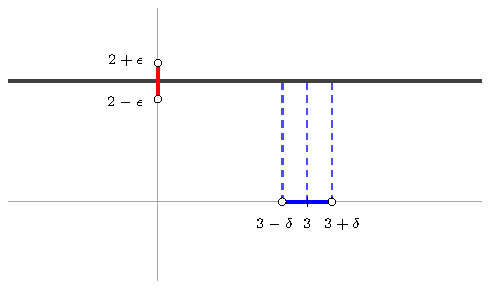
\includegraphics{figuras/limite-constante.pdf}
        \caption{Gráfica de la función $f(x)=2$. Se cumple que $\lim_{x\to 3}f(x)=2$.}
        \label{fig:4.2}
    \end{figure}

    \begin{ejemplo}[Aplicación de la definición de límite]\label{ejm:41}
        Sea $f(x)=x$. Prueba
        que $\lim_{x\to 1}f(x)=1$.

        \textbf{Solución.} Según el punto número 4 de la observación~\ref{obs:8}, debemos probar
        que para todo $\epsilon>0$, existe $\delta>0$ tal que si $0<|x-1|<\delta$, entonces
        $|f(x)-1|<\epsilon$. Sea $\epsilon>0$ y tomemos $\delta=\epsilon$ (cualquier $0<\delta\leq\epsilon$ sirve, véase
        la figura~\ref{fig:4.3}). Notemos que si $0<|x-1|<\delta$, entonces
        \begin{equation*}
            |f(x)-1|=|x-1|<\delta=\epsilon,
        \end{equation*}
        por lo tanto, por la definición~\ref{def:28} obtenemos que $\lim_{x\to 1}f(x)=1$.
    \end{ejemplo}

    \begin{figure}[H]
        \centering
        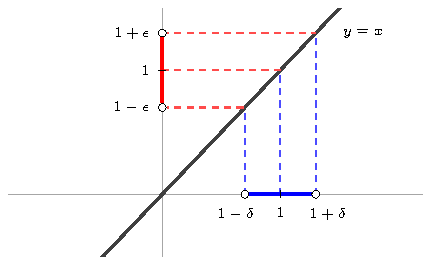
\includegraphics{figuras/limite-identidad.pdf}
        \caption{Gráfica de la función $f(x)=x$. Se cumple que $\lim_{x\to 1}f(x)=1$.}
        \label{fig:4.3}
    \end{figure}

    \begin{ejemplo}[Negación de la definición de límite]\label{ejm:42}
        Sea $f(x)=3$. Prueba,
        usando la negación de la definición~\ref{def:28}, que es falso que $\lim_{x\to 2}f(x)=5$.

        \textbf{Solución.}\footnote{Podemos probar que es falso que $\lim_{x\to 2}f(x)=5$ probando que $\lim_{x\to 2}f(x)=3$ y
        utilizando la unicidad del límite (proposición~\ref{prop:32}), sin embargo, la intención de este ejercicio
        es probar lo afirmado utilizando la negación de la definición de límite.} Según el punto número 5 de la observación~\ref{obs:8}, debemos probar
        que existe $\epsilon>0$ tal que para toda $\delta>0$, existe $x\in\R$ tal que $0<|x-2|<\delta$ y
        $|f(x)-5|\geq\epsilon$. Sea $\epsilon=1$ y tomemos $\delta>0$. Notemos que el punto $x=2+\delta/2$
        cumple que $0<|x-2|<\delta$ y
        \begin{equation*}
            |f(x)-5|=|3-5|=2\geq\epsilon,
        \end{equation*}
        por lo tanto, es falso que $\lim_{x\to 2}f(x)=5$. Notemos que el argumento anterior
        funciona con cualquier $0<\epsilon\leq 2$. Recomendamos al lector que realice un
        dibujo que clarifique la elección de $\epsilon=1$ y $x=2+\delta/2$.
    \end{ejemplo}

    \begin{ejemplo}[Negación de la definición de límite]\label{ejm:43}
        Sea $f(x)=x$. Prueba,
        usando la negación de la definición~\ref{def:28}, que es falso que $\lim_{x\to 3}f(x)=4$.

        \textbf{Solución.}\footnote{Podemos probar que es falso que $\lim_{x\to 3}f(x)=4$ probando que $\lim_{x\to 3}f(x)=3$ y
        utilizando la unicidad del límite (proposición~\ref{prop:32}), sin embargo, la intención de este ejercicio
        es probar lo afirmado utilizando la negación de la definición de límite.} Según el punto número 5 de la observación~\ref{obs:8}, debemos probar
        que existe $\epsilon>0$ tal que para toda $\delta>0$, existe $x\in\R$ tal que $0<|x-3|<\delta$
        y $|f(x)-4|\geq\epsilon$. Sea $\epsilon=1/2$ y tomemos $\delta>0$. Notemos que el punto
        $x=3-\delta/2$ cumple que $0<|x-3|<\delta$ y
        \begin{equation*}
            |f(x)-4|=|x-4|=\left|3-\frac{\delta}{2}-4\right|=1+\frac{\delta}{2}\geq\epsilon,
        \end{equation*}
        por lo tanto, es falso que $\lim_{x\to 3}f(x)=4$. Notemos que el argumento anterior
        funciona con cualquier $0<\epsilon\leq 1$. Recomendamos al lector que realice un
        dibujo que clarifique la elección de $\epsilon=1/2$ y $x=3-\delta/2$.
    \end{ejemplo}

    \begin{ejemplo}[Un límite que no existe]\label{ejm:44}
        Sea
        \begin{equation*}
            f(x)=\begin{cases}
                1, & \text{si }x\geq 0,\\
                -1, & \text{si }x<0.
            \end{cases}
        \end{equation*}
        Prueba que $\lim_{x\to 0}f(x)$ no existe (véase la figura~\ref{fig:4.4}).

        \textbf{Solución.} Debemos probar que es falso que $\lim_{x\to 0}f(x)=L$ para todo
        número real $L$. Mostraremos primero que es falso que $\lim_{x\to 0}f(x)=L$ para
        $L\geq 0$. Supongamos entonces que $L\geq 0$. Sea $\epsilon=1$ y tomemos $\delta>0$. Notemos
        que el punto $x=-\delta/2$ cumple que $0<|x-0|<\delta$ y
        \begin{align*}
            |f(x)-L|&=|-1-L|\\
            &=1+L\\
            &\geq\epsilon.
        \end{align*}
        Por lo tanto, es falso que $\lim_{x\to 0}f(x)=L$ si $L\geq 0$. La prueba de que es
        falso que $\lim_{x\to 0}f(x)=L$ para $L<0$ es similar.
    \end{ejemplo}

    \begin{figure}[H]
        \centering
        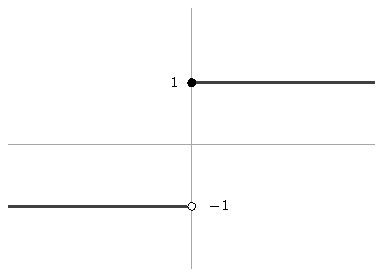
\includegraphics{figuras/escalon.pdf}
        \caption{Gráfica de la función $f(x)=\begin{cases}1, & \text{si }x\geq 0,\\ -1, & \text{si }x<0.\end{cases}$}
        \label{fig:4.4}
    \end{figure}

    \begin{ejemplo}[Otro límite que no existe]\label{ejm:45}
        Sea $f(x)=1/x$. Prueba que
        $\lim_{x\to 0}f(x)$ no existe (véase la figura~\ref{fig:4.5}).

        \textbf{Solución.} Debemos probar que es falso que $\lim_{x\to 0}f(x)=L$ para todo
        número real $L$. Mostraremos primero que es falso que $\lim_{x\to 0}f(x)=L$ si
        $L\geq 0$. Supongamos entonces que $L\geq 0$. Sea $\epsilon=1$ y tomemos $\delta>0$. Existe
        $N\in\N$ con $N>1$ tal que $N/\delta>1$. Notemos que el punto $x=-\delta/N$ cumple
        que $0<|x-0|<\delta$ y
        \begin{align*}
            |f(x)-L|&=\left|\frac{1}{(-\delta/N)}-L\right|\\
            &=\left|-\frac{N}{\delta}-L\right|\\
            &=\frac{N}{\delta}+L\\
            &>1+L\\
            &\geq\epsilon.
        \end{align*}
        Por lo tanto, es falso que $\lim_{x\to 0}f(x)=L$ si $L\geq 0$. La prueba de que es
        falso que $\lim_{x\to 0}f(x)=L$ para $L<0$ es similar.
    \end{ejemplo}

    \begin{figure}[H]
        \centering
        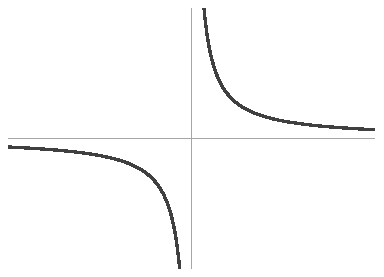
\includegraphics{figuras/reciproco.pdf}
        \caption{Gráfica de la función $f(x)=\frac{1}{x}$}
        \label{fig:4.5}
    \end{figure}

    \begin{observacion}\label{obs:9}
        Los dos ejemplos anteriores son ejemplos clásicos de funciones
        que no tienen un límite cuando $x$ se aproxima a cierto punto $p$. En
        general, si los valores $f(x)$ de una función $f$ se aproximan a un número $L_{1}$
        cuando $x$ se aproxima por la derecha a un número $p$ y si los valores de $f(x)$
        se aproximan a otro número $L_{2}$ cuando $x$ se aproxima por la izquierda al
        punto $p$, entonces $\lim_{x\to p}f(x)$ no existirá (más adelante regresaremos a este
        tema cuando veamos los límites laterales). Por otra parte, si los valores $f(x)$
        de una función $f$ crecen o decrecen arbitrariamente cuando $x$ se aproxima a
        un punto $p$, entonces $\lim_{x\to p}f(x)$ tampoco existirá.
    \end{observacion}

    Para encontrar un límite o para probar que un límite no existe, no siempre
    recurriremos a la definición~\ref{def:28}, pues probar o calcular límites con esta
    definición puede ser realmente complicado para ciertas funciones, en lugar de
    ello partiremos del conocimiento de ciertos límites elementales y a partir de
    ellos calcularemos límites más complicados.

    Antes de continuar, introduciremos algo de notación para simplificar la
    escritura. Como sabemos, es común que la regla de correspondencia de una
    función $f$ esté dada mediante una ecuación. En este caso, en la expresión
    $\lim_{x\to p}f(x)$ algunas veces sustituiremos a $f(x)$ por la expresión algebraica
    que la define, por ejemplo, si $f(x)=x^{2}$, escribiremos $\lim_{x\to p}x^{2}$ en lugar de
    $\lim_{x\to p}f(x)$.

    \begin{proposicion}[Límites básicos]\label{prop:33}
        En lo que sigue $c$ es una constante. En
        el inciso (d) suponemos que $p\in\R$ si $n$ es impar y que $p>0$ si $n$ es par. Se
        cumple lo siguiente:
        \begin{enumerate}[nosep]
            \item $\displaystyle\lim_{x\to p}c=c$.
            \item $\displaystyle\lim_{x\to p}x=p$.
            \item $\displaystyle\lim_{x\to p}|x|=|p|$.
            \item $\displaystyle\lim_{x\to p}\sqrt[n]{x}=\sqrt[n]{p}$.
        \end{enumerate}
    \end{proposicion}

    \begin{proof}
        Las demostraciones de los incisos (a) y (b) son similares a las
        demostraciones de los ejemplos~\ref{ejm:40} y~\ref{ejm:41}, respectivamente. Dejamos al lector
        que complete los detalles. La demostración de (c) se deduce de la desigualdad
        \begin{equation*}
            \big||x|-|p|\big|\leq|x-p|
        \end{equation*}
        (la prueba de esta desigualdad se deja a cargo del lector, véase el ejercicio~\ref{ej:132}).
        En efecto, dado $\epsilon>0$, al tomar $\delta=\epsilon$ obtenemos que si $0<|x-p|<\delta$,
        entonces
        \begin{equation*}
            \big||x|-|p|\big|\leq|x-p|<\delta=\epsilon,
        \end{equation*}
        de lo cual obtenemos (c). Resta probar (d). Sea $\epsilon>0$. En lo que resta
        de la demostración las $x$ que se consideran pertenecen al dominio de $\sqrt[n]{x}$.
        Examinaremos dos casos, $p=0$ y $p\neq 0$.

        Caso 1. $p=0$. Tomemos $\delta=\epsilon^{n}$. Luego, si $0<|x|<\delta$, entonces\footnote{Aquí utilizamos que $n$ es impar, pues $p=0$. Además, utilizamos que si $0\leq x<y$,
        entonces $x^{1/n}<y^{1/n}$ (véase el ejercicio~\ref{ej:60} de la sección~\ref{sec:naturales}).}
        \begin{equation*}
            \left|x^{\frac{1}{n}}\right|=|x|^{\frac{1}{n}}<\delta^{\frac{1}{n}}=\epsilon,
        \end{equation*}
        de lo cual obtenemos (d).

        Caso 2. $p\neq 0$. Notemos primero que
        \begin{equation*}
            \left(x^{\frac{1}{2}}-p^{\frac{1}{2}}\right)\left(x^{\frac{1}{2}}+p^{\frac{1}{2}}\right)=x-p,
        \end{equation*}
        que
        \begin{equation*}
            \left(x^{\frac{1}{3}}-p^{\frac{1}{3}}\right)\left(x^{\frac{2}{3}}+x^{\frac{1}{3}}p^{\frac{1}{3}}+p^{\frac{2}{3}}\right)=x-p,
        \end{equation*}
        y que en general, si $n$ es un número natural,
        \begin{equation*}
            \left(x^{\frac{1}{n}}-p^{\frac{1}{n}}\right)\left(x^{\frac{n-1}{n}}+x^{\frac{n-2}{n}}p^{\frac{1}{n}}+\cdots+x^{\frac{1}{n}}p^{\frac{n-2}{n}}+p^{\frac{n-1}{n}}\right)=x-p.
        \end{equation*}
        Sea
        \begin{equation*}
            C(x)=x^{\frac{n-1}{n}}+x^{\frac{n-2}{n}}p^{\frac{1}{n}}+\cdots+x^{\frac{1}{n}}p^{\frac{n-2}{n}}+p^{\frac{n-1}{n}}.
        \end{equation*}
        Si $p>0$ y $x>0$, es claro que todos los sumandos de $C(x)$ son positivos.
        Si $p<0$ y $x<0$, ocurre lo mismo, pues en este caso estamos suponiendo
        que $n$ es impar. Tomemos $\delta_{1}>0$ suficientemente pequeño de manera que
        si $0<|x-p|<\delta_{1}$, entonces $x$ y $p$ tienen el mismo signo. Tomemos $\delta_{2}=
        \epsilon p^{(n-1)/n}$ y $\delta=\min\{\delta_{1},\delta_{2}\}$. Luego, si $x$ está en el dominio de la función $x^{1/n}$
        y $0<|x-p|<\delta$, entonces
        \begin{equation*}
            \left|\sqrt[n]{x}-\sqrt[n]{p}\right|=\left|\frac{x-p}{C(x)}\right|=\frac{|x-p|}{C(x)}<\frac{\delta}{p^{\frac{n-1}{n}}}\leq\frac{\delta_{2}}{p^{\frac{n-1}{n}}}=\epsilon.
        \end{equation*}
        Por lo tanto, obtenemos (d).
    \end{proof}

    La prueba de las dos proposiciones siguientes se puede consultar, por ejemplo,
    en \cite{nunez2020calculoII}.

    \begin{proposicion}[Límites de las funciones trigonométricas]\label{prop:34}
        En lo
        que sigue $p$ pertenece al dominio de las funciones trigonométricas en cuestión.
        Se cumple lo siguiente:
        \begin{enumerate}[nosep]
            \item $\displaystyle\lim_{x\to p}\sin(x)=\sin(p)$.
            \item $\displaystyle\lim_{x\to p}\cos(x)=\cos(p)$.
            \item $\displaystyle\lim_{x\to p}\tan(x)=\tan(p)$.
            \item $\displaystyle\lim_{x\to p}\cot(x)=\cot(p)$.
            \item $\displaystyle\lim_{x\to p}\sec(x)=\sec(p)$.
            \item $\displaystyle\lim_{x\to p}\csc(x)=\csc(p)$.
        \end{enumerate}
    \end{proposicion}

    \begin{proposicion}[Límites de las funciones logaritmo natural y exponencial]\label{prop:35}
        En lo que sigue $p$ pertenece al dominio de las funciones en cuestión.
        Se cumple lo siguiente:
        \begin{enumerate}[nosep]
            \item $\displaystyle\lim_{x\to p}\ln(x)=\ln(p)$.
            \item $\displaystyle\lim_{x\to p}e^{x}=e^{p}$.
        \end{enumerate}
    \end{proposicion}

    Como tal vez el lector lo habrá notado, para calcular $\lim_{x\to p}f(x)$ cuando
    $f$ es una de las funciones que aparecen en las tres proposiciones anteriores,
    simplemente hay que evaluar la función $f$ en $p$, sin embargo, cabe señalar que
    esto no se puede hacer con todas las funciones (más adelante veremos ejemplos
    de ello). Las funciones de las tres proposiciones anteriores son ejemplos de un
    tipo de funciones muy importantes llamadas funciones continuas, las cuales
    estudiaremos más adelante.

    La proposición siguiente nos dice como operar con límites.

    \begin{proposicion}[Álgebra de límites]\label{prop:36}
        \index{algebra de limites@álgebra de límites}Sean $f$ y $g$ funciones definidas en
        un intervalo abierto $I$ que contiene a $p$, excepto posiblemente en $p$. Supongamos
        que $\lim_{x\to p}f(x)$ y que $\lim_{x\to p}g(x)$ existen. Entonces
        \begin{enumerate}[nosep]
            \item $\displaystyle\lim_{x\to p}[f(x)+g(x)]=\lim_{x\to p}f(x)+\lim_{x\to p}g(x)$.
            \item $\displaystyle\lim_{x\to p}[f(x)-g(x)]=\lim_{x\to p}f(x)-\lim_{x\to p}g(x)$.
            \item $\displaystyle\lim_{x\to p}f(x)g(x)=\lim_{x\to p}f(x)\cdot\lim_{x\to p}g(x)$.
            \item $\displaystyle\lim_{x\to p}f(x)/g(x)=\lim_{x\to p}f(x)/\lim_{x\to p}g(x)$, si $\displaystyle\lim_{x\to p}g(x)\neq 0$.\footnote{El caso en que $\lim_{x\to p}g(x)=0$ lo consideraremos en las secciones~\ref{sec:limites-infinitos} y~\ref{sec:lhopital} (véanse el
            ejercicio~\ref{ej:176} y la proposición~\ref{prop:67} (regla de L'Hôpital)).}
        \end{enumerate}
    \end{proposicion}

    \begin{proof}
        Sean $\epsilon>0$, $L_{1}=\lim_{x\to p}f(x)$ y $L_{2}=\lim_{x\to p}g(x)$. El inciso
        (a) se sigue de la desigualdad siguiente (la cual, a su vez, se sigue de la
        desigualdad del triángulo)
        \begin{align*}
            |(f(x)+g(x))-(L_{1}+L_{2})|&=|(f(x)-L_{1})+(g(x)-L_{2})|\\
            &\leq|f(x)-L_{1}|+|g(x)-L_{2}|.
        \end{align*}
        En efecto, puesto que $L_{1}=\lim_{x\to p}f(x)$, existe $\delta_{1}>0$ tal que
        \begin{equation*}
            \text{si }x\in I\text{ y }0<|x-p|<\delta_{1},\text{ entonces }|f(x)-L_{1}|<\frac{\epsilon}{2}.
        \end{equation*}
        De igual manera, puesto que $L_{2}=\lim_{x\to p}g(x)$, existe $\delta_{2}>0$ tal que
        \begin{equation*}
            \text{si }x\in I\text{ y }0<|x-p|<\delta_{2},\text{ entonces }|g(x)-L_{2}|<\frac{\epsilon}{2}.
        \end{equation*}
        Definamos $\delta=\min\{\delta_{1},\delta_{2}\}$. Luego, si $x\in I$ y $0<|x-p|<\delta$, entonces
        \begin{align*}
            |(f(x)+g(x))-(L_{1}+L_{2})|&=|(f(x)-L_{1})+(g(x)-L_{2})|\\
            &\leq|f(x)-L_{1}|+|g(x)-L_{2}|\\
            &<\frac{\epsilon}{2}+\frac{\epsilon}{2}\\
            &=\epsilon.
        \end{align*}
        Por lo tanto, obtenemos (a). La prueba del inciso (b) es análoga a la del inciso
        (a). El inciso (c) se sigue de que
        \begin{align*}
            |f(x)g(x)-L_{1}L_{2}|&=|f(x)g(x)-f(x)L_{2}+f(x)L_{2}-L_{1}L_{2}|\\
            &\leq|f(x)g(x)-f(x)L_{2}|+|f(x)L_{2}-L_{1}L_{2}|\\
            &=|f(x)||g(x)-L_{2}|+|L_{2}||f(x)-L_{1}|.
        \end{align*}
        En efecto, primero tomemos $\eta>0$ tal que
        \begin{equation}\label{eq:4.4}
            (\eta+|L_{1}|)\eta+|L_{2}|\eta<\epsilon
        \end{equation}
        (la existencia de tal $\eta$ está garantizada por la propiedad arquimediana de
        los números reales). La razón de elegir $\eta$ de esta manera se verá más tarde.
        Puesto que $L_{1}=\lim_{x\to p}f(x)$, existe $\delta_{1}>0$ tal que
        \begin{equation*}
            \text{si }x\in I\text{ y }0<|x-p|<\delta_{1},\text{ entonces }|f(x)-L_{1}|<\eta
        \end{equation*}
        y, en consecuencia, si $x\in I$ y $0<|x-p|<\delta_{1}$, por la desigualdad del
        triángulo, también resulta que
        \begin{align*}
            |f(x)|&=|f(x)-L_{1}+L_{1}|\\
            &\leq|f(x)-L_{1}|+|L_{1}|\\
            &<\eta+|L_{1}|.
        \end{align*}
        Por otra parte, puesto que $L_{2}=\lim_{x\to p}g(x)$, existe $\delta_{2}>0$ tal que
        \begin{equation*}
            \text{si }x\in I\text{ y }0<|x-p|<\delta_{2},\text{ entonces }|g(x)-L_{2}|<\eta.
        \end{equation*}
        Definamos $\delta=\min\{\delta_{1},\delta_{2}\}$. Luego, si $x\in I$ y $0<|x-p|<\delta$, entonces
        \begin{align*}
            |f(x)g(x)-L_{1}L_{2}|&=|f(x)g(x)-f(x)L_{2}+f(x)L_{2}-L_{1}L_{2}|\\
            &\leq|f(x)g(x)-f(x)L_{2}|+|f(x)L_{2}-L_{1}L_{2}|\\
            &=|f(x)||g(x)-L_{2}|+|L_{2}||f(x)-L_{1}|\\
            &<(\eta+|L_{1}|)\eta+|L_{2}|\eta\\
            &<\epsilon,
        \end{align*}
        de lo cual obtenemos (c). Para probar (d), probaremos primero que
        \begin{equation}\label{eq:4.5}
            \lim_{x\to p}\frac{1}{g(x)}=\frac{1}{L_{2}}
        \end{equation}
        y, en consecuencia, por el inciso (c), tendremos que
        \begin{align*}
            \lim_{x\to p}\frac{f(x)}{g(x)}&=\lim_{x\to p}\frac{1}{g(x)}\cdot f(x)\\
            &=\frac{1}{L_{2}}\cdot L_{1}\\
            &=\frac{L_{1}}{L_{2}}.
        \end{align*}
        Para probar \eqref{eq:4.5}, notemos primero que
        \begin{equation*}
            \left|\frac{1}{g(x)}-\frac{1}{L_{2}}\right|=\left|\frac{L_{2}-g(x)}{g(x)L_{2}}\right|.
        \end{equation*}
        Sea
        \begin{equation*}
            \eta=\min\left\{\frac{|L_{2}|}{2},\frac{|L_{2}|^{2}\epsilon}{2}\right\}>0.
        \end{equation*}
        Más adelante se verá la razón de considerar este mínimo. Puesto que $\lim_{x\to p}g(x)=
        L_{2}$, existe $\delta>0$ tal que
        \begin{equation*}
            \text{si }x\in I\text{ y }0<|x-p|<\delta,\text{ entonces }|g(x)-L_{2}|<\eta.
        \end{equation*}
        Como
        \begin{equation*}
            \big||g(x)|-|L_{2}|\big|\leq|g(x)-L_{2}|,
        \end{equation*}
        si $x\in I$ y $0<|x-p|<\delta$, se tiene entonces que
        \begin{equation*}
            \big||g(x)|-|L_{2}|\big|<\eta.
        \end{equation*}
        La desigualdad anterior implica que
        \begin{equation}\label{eq:4.6}
            -\frac{|L_{2}|}{2}\leq-\eta<|g(x)|-|L_{2}|<\eta\leq\frac{|L_{2}|}{2},
        \end{equation}
        lo cual, a su vez, al sumar $|L_{2}|$ a todas las desigualdades de \eqref{eq:4.6}, implica que
        \begin{equation*}
            \frac{|L_{2}|}{2}<|g(x)|<3\frac{|L_{2}|}{2}
        \end{equation*}
        y, en consecuencia, que
        \begin{equation*}
            \frac{1}{|g(x)|}<\frac{2}{|L_{2}|}.
        \end{equation*}
        Así, si $x\in I$ y $0<|x-p|<\delta$, entonces
        \begin{align*}
            \left|\frac{1}{g(x)}-\frac{1}{L_{2}}\right|&=\left|\frac{L_{2}-g(x)}{g(x)L_{2}}\right|\\
            &=\frac{1}{|L_{2}|}\frac{1}{|g(x)|}|L_{2}-g(x)|\\
            &<\frac{1}{|L_{2}|}\frac{2}{|L_{2}|}\frac{|L_{2}|^{2}\epsilon}{2}\\
            &=\epsilon.
        \end{align*}
        Por lo tanto, obtenemos \eqref{eq:4.5} y, en consecuencia, como comentamos, (d).
    \end{proof}

    En otras palabras, la proposición anterior dice lo siguiente:
    \begin{itemize}[nosep,label=$\blacksquare$]
        \item El límite de una suma es la suma de los límites.
        \item El límite de una resta es la resta de los límites.
        \item El límite de un producto es el producto de los límites.
        \item El límite de un cociente es el cociente de los límites (si el límite del
        denominador no es cero).
    \end{itemize}

    \begin{observacion}\label{obs:10}
        Conviene en este momento notar lo siguiente:
        \begin{enumerate}
            \item Notemos que si $c$ es una constante, entonces del inciso (c) del álgebra de
            límites y del inciso (a) de la proposición~\ref{prop:33} obtenemos que si $\lim_{x\to p}f(x)$
            existe, entonces
            \begin{equation*}
                \lim_{x\to p}cf(x)=\left(\lim_{x\to p}c\right)\left(\lim_{x\to p}f(x)\right)=c\cdot\lim_{x\to p}f(x).
            \end{equation*}
            \item ¿Qué sucede si en el inciso (d) del álgebra de límites se tiene que
            $\lim_{x\to p}g(x)=0$? Surgen dos casos, cuando $\lim_{x\to p}f(x)\neq 0$ y cuando
            $\lim_{x\to p}f(x)=0$. En el primer caso resulta que $\lim_{x\to p}f(x)/g(x)$ no
            existe, pues si suponemos que tal límite existe, entonces por el inciso (c)
            del álgebra de límites obtenemos que
            \begin{equation*}
                \lim_{x\to p}f(x)=\lim_{x\to p}g(x)\frac{f(x)}{g(x)}=\lim_{x\to p}g(x)\lim_{x\to p}\frac{f(x)}{g(x)}=0,
            \end{equation*}
            lo cual es una contradicción. El segundo caso lo trataremos cuando estudiemos
            la regla de L'Hôpital en la sección~\ref{sec:lhopital}.
        \end{enumerate}
    \end{observacion}

    Con el álgebra de límites y con los límites señalados en las proposiciones~\ref{prop:33},
    \ref{prop:34} y~\ref{prop:35} podemos calcular límites más complejos como lo muestran los
    ejemplos siguientes.

    \begin{ejemplo}\label{ejm:46}
        $\lim_{x\to p}x^{n}=p^{n}$.

        En efecto, por el inciso (b) de la proposición~\ref{prop:33} sabemos que $\lim_{x\to p}x=p$.
        En consecuencia, por el inciso (c) de la proposición~\ref{prop:36} sabemos que
        \begin{equation*}
            \lim_{x\to p}x^{n}=\left(\lim_{x\to p}x\right)^{n}=p^{n}.\finej
        \end{equation*}
    \end{ejemplo}

    \begin{ejemplo}\label{ejm:47}
        Si $c$ es una constante, entonces $\lim_{x\to p}cx^{n}=c\cdot p^{n}$.

        En efecto, como $c$ es una constante, por la observación~\ref{obs:10}, obtenemos que
        \begin{equation*}
            \lim_{x\to p}cx^{n}=c\left(\lim_{x\to p}x^{n}\right)=c\cdot p^{n}.\finej
        \end{equation*}
    \end{ejemplo}

    \begin{ejemplo}[Límite de un polinomio]\label{ejm:48}
        Si $P(x)$ es un polinomio, entonces
        \begin{equation*}
            \lim_{x\to p}P(x)=P(p).
        \end{equation*}
        En efecto, como $P(x)$ es de la forma
        \begin{equation*}
            P(x)=a_{0}+a_{1}x+a_{2}x^{2}+\cdots+a_{n}x^{n},
        \end{equation*}
        donde $a_{0},a_{1},\ldots,a_{n}$ son constantes, entonces por el inciso (a) de la proposición~\ref{prop:36}
        y lo que mostramos en los dos ejemplos anteriores obtenemos que
        \begin{align*}
            \lim_{x\to p}P(x)&=\lim_{x\to p}\left[a_{0}+a_{1}x+a_{2}x^{2}+\cdots+a_{n}x^{n}\right]\\
            &=\lim_{x\to p}a_{0}+\lim_{x\to p}a_{1}x+\lim_{x\to p}a_{2}x^{2}+\cdots+\lim_{x\to p}a_{n}x^{n}\\
            &=a_{0}+a_{1}p+a_{2}p^{2}+\cdots+a_{n}p^{n}\\
            &=P(p).
        \end{align*}
        Así, para calcular $\lim_{x\to p}P(x)$ cuando $P$ es un polinomio también basta
        evaluar $P$ en $p$.
    \end{ejemplo}

    Con los resultados de esta subsección podemos obtener límites que en
    apariencia parecen difíciles de calcular pero que en realidad son sencillos.

    \begin{ejemplo}\label{ejm:49}
        Calcula
        \begin{equation*}
            \lim_{x\to 0}\cos(x)\left(3x^{7}-5x+4-e^{x}\right)\frac{18|x|+4}{1+x^{2}}.
        \end{equation*}

        \textbf{Solución.} Según los resultados de esta sección tenemos que
        \begin{align*}
            &\lim_{x\to 0}\cos(x)\left(3x^{7}-5x+4-e^{x}\right)\frac{18|x|+4}{1+x^{2}}=\\
            &=\left[\lim_{x\to 0}\cos(x)\right]\left[\lim_{x\to 0}\left(3x^{7}-5x+4-e^{x}\right)\right]\frac{\lim_{x\to 0}(18|x|+4)}{\lim_{x\to 0}\left(1+x^{2}\right)}\\
            &=1\cdot 3\,\frac{0+4}{1}\\
            &=12.\finej
        \end{align*}
    \end{ejemplo}

    Todos los límites que hemos encontrado hasta este momento, si existen,
    tienen la propiedad de que $\lim_{x\to p}f(x)=f(p)$ (esta propiedad se expresa
    diciendo que $f$ es continua en $p$; más adelante estudiaremos a las funciones
    continuas), es decir, para calcular $\lim_{x\to p}f(x)$ basta con evaluar $f$ en $p$. El
    ejemplo siguiente muestra que esto no siempre es posible.

    \begin{ejemplo}[Una función $f$ tal que $\lim_{x\to p}f(x)$ existe y, sin embargo, es distinto de $f(p)$]\label{ejm:50}
        Consideremos la función dada por
        \begin{equation*}
            f(x)=\begin{cases}
                1, & \text{si }x\neq 3,\\
                2, & \text{si }x=3
            \end{cases}
        \end{equation*}
        (la gráfica de $f$ se muestra en la figura~\ref{fig:4.6}). Entonces
        \begin{equation*}
            \lim_{x\to 3}f(x)=1\neq 2=f(3).
        \end{equation*}
        En efecto, basta mostrar que $\lim_{x\to 3}f(x)=1$. Sea $\epsilon>0$ y tomemos $\delta=1$.
        Luego, si $0<|x-3|<\delta$, entonces $x\neq 3$ y, en consecuencia, $f(x)=1$. Por
        lo cual
        \begin{equation*}
            |f(x)-1|=|1-1|=0<\epsilon.
        \end{equation*}
        De la definición~\ref{def:28} obtenemos que $\lim_{x\to 3}f(x)=1$.
    \end{ejemplo}

    \begin{figure}[H]
        \centering
        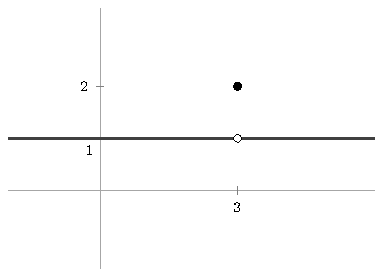
\includegraphics{figuras/funcion-salto-punto.pdf}
        \caption{Gráfica de la función $f(x)=\begin{cases}1, & \text{si }x\neq 3,\\ 2, & \text{si }x=3.\end{cases}$}
        \label{fig:4.6}
    \end{figure}

    Puesto que la definición de $\lim_{x\to p}f(x)$ no requiere que $f$ esté definida en
    $p$, tenemos el resultado siguiente.

    \begin{proposicion}\label{prop:37}
        Sean $f$ y $g$ funciones definidas en un intervalo abierto $I$
        que contiene a $p$, excepto posiblemente en $p$. Si
        \begin{equation*}
            f(x)=g(x)\ \text{para todo }x\in I\text{ con }x\neq p
        \end{equation*}
        y $\lim_{x\to p}g(x)$ existe, entonces $\lim_{x\to p}f(x)$ también existe y
        \begin{equation*}
            \lim_{x\to p}f(x)=\lim_{x\to p}g(x).
        \end{equation*}
    \end{proposicion}

    Como una aplicación de la proposición anterior veamos el ejemplo siguiente.

    \begin{ejemplo}[Límites por factorización]\label{ejm:51}
        \index{limites por factorizacion@límites por factorización}Calcula
        \begin{equation}\label{eq:4.7}
            \lim_{x\to 1}\frac{x^{3}-x^{2}}{x-1}.
        \end{equation}

        \textbf{Solución.} Notemos primero que para calcular este límite no podemos usar
        el inciso (d) del álgebra de límites, pues el límite del denominador de \eqref{eq:4.7}
        cuando $x$ tiende a $1$ es $0$. Por otra parte, notemos que si $x\neq 1$, al factorizar
        el numerador de \eqref{eq:4.7} obtenemos que
        \begin{equation*}
            \frac{x^{3}-x^{2}}{x-1}=\frac{x^{2}(x-1)}{x-1}=x^{2}\text{ si }x\neq 1.
        \end{equation*}
        Las funciones $f(x)=\left(x^{3}-x^{2}\right)/(x-1)$ y $g(x)=x^{2}$ son iguales en todo
        punto, excepto en $x=1$, pues $g(1)=1$ y $f$ ni siquiera está definida en
        $x=1$. Las gráficas de $f$ y $g$ se muestran en la figura~\ref{fig:4.7}. Por la proposición~\ref{prop:37}
        obtenemos que
        \begin{equation*}
            \lim_{x\to 1}\frac{x^{3}-x^{2}}{x-1}=\lim_{x\to 1}x^{2}=1.\finej
        \end{equation*}
    \end{ejemplo}

    \begin{figure}[H]
        \centering
        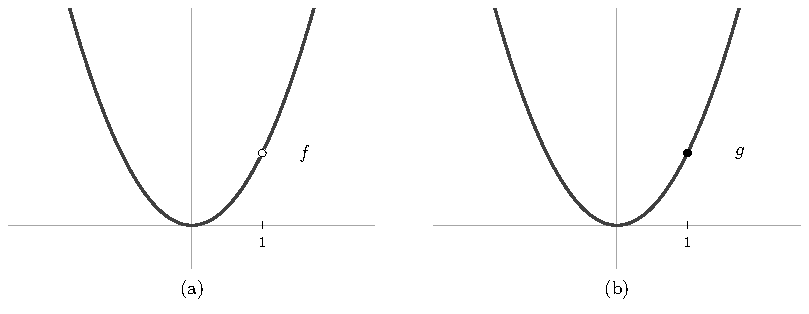
\includegraphics{figuras/factorizacion.pdf}
        \caption{Gráficas de las funciones $f(x)=\left(x^{3}-x^{2}\right)/(x-1)$ y $g(x)=x^{2}$. La función
        $f$ no está definida en $x=1$.}
        \label{fig:4.7}
    \end{figure}

    \begin{ejemplo}[Otro límite por factorización]\label{ejm:52}
        Calcula
        \begin{equation*}
            \lim_{x\to -3}\frac{2x^{2}+8x+6}{x^{3}+3x^{2}+x+3}.
        \end{equation*}

        \textbf{Solución.} Como
        \begin{equation*}
            \frac{2x^{2}+8x+6}{x^{3}+3x^{2}+x+3}=\frac{(x+3)(2x+2)}{\left(x^{2}+1\right)(x+3)}=\frac{2x+2}{x^{2}+1}\text{ si }x\neq -3,
        \end{equation*}
        entonces por la proposición~\ref{prop:37} obtenemos que
        \begin{equation*}
            \lim_{x\to -3}\frac{2x^{2}+8x+6}{x^{3}+3x^{2}+x+3}=\lim_{x\to -3}\frac{2x+2}{x^{2}+1}=-\frac{4}{10}.\finej
        \end{equation*}
    \end{ejemplo}

    Ahora enunciaremos un resultado clásico de límites, el famoso lema del
    sándwich.

    \begin{proposicion}[Lema del sándwich, versión 1]\label{prop:38}
        \index{lema del sandwich@lema del sándwich}Sean $f$ y $g$ funciones
        definidas en un intervalo abierto $I$ que contiene a $p$, excepto posiblemente en
        $p$. Si
        \begin{equation}\label{eq:4.8}
            0\leq f(x)\leq g(x)\ \text{ para todo }x\in I\backslash\{p\}
        \end{equation}
        y
        \begin{equation*}
            \lim_{x\to p}g(x)=0,
        \end{equation*}
        entonces
        \begin{equation*}
            \lim_{x\to p}f(x)=0.
        \end{equation*}
    \end{proposicion}

    \begin{proof}
        Sea $\epsilon>0$. Puesto que $\lim_{x\to p}g(x)=0$, existe $\delta>0$ tal que
        si $x\in I$ y $0<|x-p|<\delta$, entonces $|g(x)|<\epsilon$. En consecuencia, por \eqref{eq:4.8}, si
        $x\in I$ y $0<|x-p|<\delta$, entonces
        \begin{equation*}
            |f(x)|\leq|g(x)|<\epsilon.
        \end{equation*}
        Por lo tanto, $\lim_{x\to p}f(x)=0$.
    \end{proof}

    El lema del sándwich es equivalente a la proposición siguiente, también
    conocida como lema del sándwich (véase el ejercicio~\ref{ej:149}).

    \begin{proposicion}[Lema del sándwich, versión 2]\label{prop:39}
        Sean $f$, $g$ y $h$ funciones
        definidas en un intervalo abierto $I$ que contiene a $p$, excepto posiblemente
        en $p$. Si
        \begin{equation*}
            f(x)\leq g(x)\leq h(x)\ \text{ para todo }x\in I\backslash\{p\}
        \end{equation*}
        y
        \begin{equation*}
            \lim_{x\to p}f(x)=L=\lim_{x\to p}h(x),
        \end{equation*}
        entonces
        \begin{equation*}
            \lim_{x\to p}g(x)=L.
        \end{equation*}
    \end{proposicion}

    Como una aplicación del lema del sándwich veamos el ejemplo siguiente.

    \begin{ejemplo}\label{ejm:53}
        Se cumple que
        \begin{equation*}
            \lim_{x\to 0}\frac{\sin(x)}{x}=1.
        \end{equation*}
        Notemos que para calcular este límite no podemos usar el inciso (d) de la
        proposición~\ref{prop:36}, pues el límite del denominador es $0$. Este límite también lo
        calcularemos usando técnicas distintas en la sección~\ref{sec:lhopital}. Más adelante, en la
        sección~\ref{subsec:monotonas-derivada}, mostraremos que
        \begin{equation}\label{eq:4.9}
            \sin(x)\leq x\leq\tan(x)\ \text{ para toda }x\in[0,\pi/2)
        \end{equation}
        y que
        \begin{equation}\label{eq:4.10}
            \sin(x)\geq x\geq\tan(x)\ \text{ para toda }x\in(-\pi/2,0].
        \end{equation}
        Al dividir \eqref{eq:4.9} y \eqref{eq:4.10} entre $\sin(x)$ resulta que
        \begin{equation*}
            \cos(x)\leq\frac{\sin(x)}{x}\leq 1\ \text{ para toda }x\in(-\pi/2,\pi/2)\backslash\{0\}.
        \end{equation*}
        Luego, como $\lim_{x\to 0}\cos(x)=1$ y $\lim_{x\to 0}1=1$, por el lema del sándwich
        obtenemos que $\lim_{x\to 0}\sin(x)/x=1$.
    \end{ejemplo}

    Para mostrar otra aplicación (proposición~\ref{prop:40}) del lema del sándwich
    introduciremos primero el concepto de función acotada.

    \begin{definicion}[Función acotada]\label{def:29}
        Sean $f$ una función y $A\subset\dom(f)$.
        \begin{enumerate}[nosep]
            \item Diremos que $f$ \textit{es acotada en} $A$ si $f(A)$ es un conjunto acotado, es decir,
            si existe $M>0$ tal que
            \begin{equation*}
                |f(x)|\leq M\quad\text{para todo }x\in A
            \end{equation*}
            (véase el ejercicio~\ref{ej:136}).
            \item Diremos que $f$ es \textit{acotada}\index{funcion acotada@función acotada} si $f$ es acotada en su dominio.
        \end{enumerate}
    \end{definicion}

    Así, una función $f$ es acotada si existe $M>0$ tal que su gráfica está
    contenida en la «banda» $\R\times[-M,M]$ del plano cartesiano (véase la figura~\ref{fig:4.8}).
    Por ejemplo, las funciones constantes, la función $\sin(x)$ y la función
    $\cos(x)$ son acotadas.

    \begin{figure}[H]
        \centering
        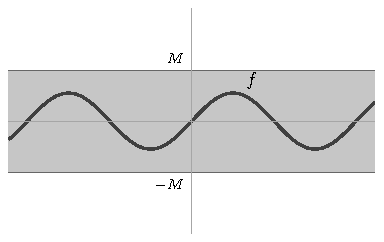
\includegraphics{figuras/funcion-acotada.pdf}
        \caption{Una función $f$ acotada: existe $M>0$ tal que la gráfica de $f$ está contenida
        en la «banda» $\R\times[-M,M]$ (en color gris) del plano cartesiano.}
        \label{fig:4.8}
    \end{figure}

    \begin{proposicion}\label{prop:40}
        Sean $f$ y $g$ funciones definidas en un intervalo abierto $I$
        que contiene a $p$, excepto posiblemente en $p$. Muestra que si $\lim_{x\to p}f(x)=0$
        y $g$ es acotada, entonces $\lim_{x\to p}f(x)g(x)=0$.
    \end{proposicion}

    Aunque sencilla, la proposición anterior, cuya prueba dejamos a cargo del
    lector (véase el ejercicio~\ref{ej:150}), nos será de utilidad en varias ocasiones.

    Terminamos esta sección estudiando el límite de una función compuesta.

    \begin{proposicion}[Límite de una función compuesta]\label{prop:41}
        Sean $g$ una función
        definida en un intervalo abierto $I$ que contiene a $p$, excepto posiblemente
        en $p$, y $f$ una función definida en un intervalo abierto $J$ que contiene a $L$.
        Supongamos que $g(I\backslash\{p\})\subset J$, de manera que la composición $f\circ g$ está definida
        en $I$, excepto posiblemente en $p$. Si $\lim_{x\to p}g(x)=L$ y $\lim_{x\to L}f(x)=f(L)$,
        entonces
        \begin{equation*}
            \lim_{x\to p}f(g(x))=f(L).
        \end{equation*}
    \end{proposicion}

    \begin{proof}
        Sea $\epsilon>0$. Puesto que $\lim_{x\to L}f(x)=f(L)$, existe $\delta>0$ tal
        que
        \begin{equation}\label{eq:4.11}
            \text{si }x\in J\text{ y }|x-L|<\delta,\text{ entonces }|f(x)-f(L)|<\epsilon.
        \end{equation}
        Por otra parte, como $\lim_{x\to p}g(x)=L$, existe $\delta_{1}>0$ tal que
        \begin{equation}\label{eq:4.12}
            \text{si }x\in I\text{ y }0<|x-p|<\delta_{1},\text{ entonces }|g(x)-L|<\delta.
        \end{equation}
        En consecuencia, si $x\in I$ y $0<|x-p|<\delta_{1}$, entonces por \eqref{eq:4.12} y \eqref{eq:4.11}
        obtenemos que
        \begin{equation*}
            |f(g(x))-f(L)|<\epsilon,
        \end{equation*}
        que es lo que queríamos probar.
    \end{proof}

    La condición de que $\lim_{x\to L}f(x)=f(L)$ en la proposición~\ref{prop:41} se expresa
    diciendo que la función $f$ es continua en $L$ (más adelante estudiaremos a las
    funciones continuas). Si en la proposición~\ref{prop:41} en lugar de pedir que
    $\lim_{x\to L}f(x)=f(L)$ solamente pedimos que $\lim_{x\to L}f(x)=M$, ¿se
    cumplirá que $\lim_{x\to p}f(g(x))=M$ (véase el ejercicio~\ref{ej:151})?

    \begin{ejemplo}\label{ejm:54}
        Para ilustrar la proposición anterior calculemos $\lim_{x\to 2}\ln\left(x^{2}-3\right)$.
        Notemos que este límite no lo podemos calcular utilizando la proposición~\ref{prop:36}
        y los límites conocidos hasta este momento. Consideremos a las funciones
        $g(x)=x^{2}-3$ y $f(x)=\ln(x)$. Como $\lim_{x\to 2}g(x)=1$ y $\lim_{x\to 1}f(x)=f(1)$,
        entonces por la proposición~\ref{prop:41} se tiene que
        \begin{equation*}
            \lim_{x\to 2}\ln\left(x^{2}-3\right)=\lim_{x\to 2}f(g(x))=f(1)=0.\finej
        \end{equation*}
    \end{ejemplo}

    \par\avoidorphan{6}\subsection*{Ejercicios}

    \begin{ejercicio}\label{ej:129}
        A partir de la definición del valor absoluto de un número,
        prueba la proposición~\ref{prop:30}.
    \end{ejercicio}

    \begin{ejercicio}\label{ej:130}
        A partir de la definición del valor absoluto de un número,
        prueba la proposición~\ref{prop:31}.
    \end{ejercicio}

    \begin{ejercicio}[Desigualdad del triángulo generalizada]\label{ej:131}
        \index{desigualdad del triangulo generalizada@desigualdad del triángulo generalizada}Prueba que si
        $n\in\N$ y $x_{1},\ldots,x_{n}\in\R$, entonces
        \begin{equation*}
            |x_{1}+\cdots+x_{n}|\leq|x_{1}|+\cdots+|x_{n}|.
        \end{equation*}
        \sugerencia Usa el principio de inducción matemática y ten presente la
        desigualdad del triángulo.
    \end{ejercicio}

    \begin{ejercicio}\label{ej:132}
        Prueba que para todo par de números $x$ y $y$ se cumple lo
        siguiente:
        \begin{multicols}{2}
        \begin{enumerate}[nosep]
            \item $|x-y|\leq|x|+|y|$.
            \item $|x|-|y|\leq|x-y|$.
            \item $\big||x|-|y|\big|\leq|x-y|$.
        \end{enumerate}
        \end{multicols}
        \sugerencia Trata de usar la desigualdad del triángulo.
    \end{ejercicio}

    \begin{ejercicio}\label{ej:133}
        Sean $x$ y $y$ números reales. Prueba lo siguiente:
        \begin{multicols}{2}
        \begin{enumerate}[nosep]
            \item $\left|\frac{1}{x}\right|=\frac{1}{|x|}$, si $x\neq 0$.
            \item $\frac{|x|}{|y|}=\left|\frac{x}{y}\right|$, si $y\neq 0$.
        \end{enumerate}
        \end{multicols}
        \sugerencia Recuerda como se definió la división y usa la unicidad del
        inverso multiplicativo.
    \end{ejercicio}

    \begin{ejercicio}\label{ej:134}
        Dado $p\in\R$ y $\delta>0$, bosqueja sobre la recta numérica el
        conjunto de los números reales $x$ que cumplen las condiciones siguientes:
        \begin{multicols}{2}
        \begin{enumerate}[nosep]
            \item $0<|x-p|$.
            \item $|x-p|<\delta$.
            \item $0<|x-p|<\delta$.
        \end{enumerate}
        \end{multicols}
    \end{ejercicio}

    \begin{ejercicio}\label{ej:135}
        Prueba que si $a\leq x\leq b$, entonces $|x|\leq\max\{|a|,|b|\}$.
    \end{ejercicio}

    \begin{ejercicio}\label{ej:136}
        Sea $A\subset\R$. Prueba que $A$ es acotado ssi existe $M>0$ tal
        que
        \begin{equation*}
            |x|\leq M,\ \text{para todo }x\in A.
        \end{equation*}
    \end{ejercicio}

    \begin{ejercicio}\label{ej:137}
        Sean $f$ una función y $A,B\subset\dom(f)$.
        \begin{enumerate}[nosep]
            \item Prueba que si $A\subset B$ y $f$ es acotada en $B$, entonces $f$ es acotada en $A$.
            \item Prueba que si $f$ es acotada tanto en $A$ como en $B$, entonces $f$ es acotada en
            $A\cup B$.
        \end{enumerate}
    \end{ejercicio}

    \begin{ejercicio}\label{ej:138}
        Sean $f$ y $g$ funciones con un dominio común $D$. Prueba que
        si $f$ y $g$ son acotadas, entonces $f+g$, $f-g$ y $fg$ son acotadas. Si está definido
        el cociente $f/g$ en $D$, ¿será $f/g$ acotada?
    \end{ejercicio}

    \begin{ejercicio}\label{ej:139}
        Prueba, usando la definición~\ref{def:28}, que:
        \begin{multicols}{2}
        \begin{enumerate}[nosep]
            \item $\lim_{x\to 1}x+2=3$.
            \item $\lim_{x\to 2}3x=6$.
            \item $\lim_{x\to -1}4x+5=1$.
            \item $\lim_{x\to 2}x^{2}-1=3$.
            \item $\lim_{x\to 1}3x^{2}+2=5$.
        \end{enumerate}
        \end{multicols}
    \end{ejercicio}

    \begin{ejercicio}\label{ej:140}
        Prueba, usando la negación de la definición~\ref{def:28}, que es \textbf{falso}
        que:
        \begin{multicols}{2}
        \begin{enumerate}[nosep]
            \item $\lim_{x\to 1}x+2=5$.
            \item $\lim_{x\to 2}3x=-1$.
            \item $\lim_{x\to -1}4x+5=0$.
            \item $\lim_{x\to 2}x^{2}-1=2$.
            \item $\lim_{x\to 1}3x^{2}+2=4$.
        \end{enumerate}
        \end{multicols}
    \end{ejercicio}

    \begin{ejercicio}\label{ej:141}
        Calcula los límites siguientes:
        \begin{multicols}{2}
        \begin{enumerate}[nosep]
            \item $\lim_{x\to 1}(3x^{3}-2x^{2}+4)$.
            \item $\lim_{x\to 8}(x+2)\sqrt[3]{x}$.
            \item $\lim_{x\to 2}\frac{2x-3}{x+5}+(x-2)\sin(x)$.
            \item $\lim_{x\to 1}\left(x^{2}-1\right)e^{x}+\frac{\ln(x)+1}{1+x^{2}}$.
        \end{enumerate}
        \end{multicols}
    \end{ejercicio}

    \begin{ejercicio}\label{ej:142}
        Calcula los límites siguientes:
        \begin{multicols}{2}
        \begin{enumerate}[nosep]
            \item $\lim_{x\to 1}\frac{x^{2}+2x-3}{x-1}$.
            \item $\lim_{x\to -1}\frac{x^{2}+4x+3}{x+1}$.
            \item $\lim_{x\to -2}\frac{x^{3}+2x^{2}+x+2}{x+2}$.
            \item $\lim_{x\to 3}\frac{x^{3}-x^{2}-9x+9}{x-3}$.
        \end{enumerate}
        \end{multicols}
    \end{ejercicio}

    \begin{ejercicio}\label{ej:143}
        Calcula los límites siguientes:
        \begin{multicols}{2}
        \begin{enumerate}[nosep]
            \item $\lim_{x\to 0}\cos\left(x^{2}+1\right)$.
            \item $\lim_{x\to -5}\ln(x+6)$.
            \item $\lim_{x\to 4}\left(\sqrt{x}-5\right)^{1000000}$.
            \item $\lim_{x\to 1}e^{1-x^{2}}$.
        \end{enumerate}
        \end{multicols}
    \end{ejercicio}

    \begin{ejercicio}\label{ej:144}
        Sea
        \begin{equation*}
            f(x)=\begin{cases}
                1, & \text{si }x\geq 0,\\
                -1, & \text{si }x<0.
            \end{cases}
        \end{equation*}
        Calcula $\lim_{x\to 3}f(x)$ (argumenta tu respuesta).
    \end{ejercicio}

    \begin{ejercicio}\label{ej:145}
        Prueba que $\lim_{x\to p}f(x)=L$ ssi $\lim_{x\to p}f(x)-L=0$.
    \end{ejercicio}

    \begin{ejercicio}\label{ej:146}
        Prueba que $\lim_{x\to p}f(x)=0$ ssi $\lim_{x\to p}|f(x)|=0$.
    \end{ejercicio}

    \begin{ejercicio}\label{ej:147}
        Prueba que $\lim_{x\to p}f(x)=L$ ssi $\lim_{h\to 0}f(p+h)=L$.
    \end{ejercicio}

    \begin{ejercicio}[Límites y desigualdades]\label{ej:148}
        Considera dos funciones $f$ y $g$
        definidas en un intervalo abierto $I$ que contiene a $p$ tales que $\lim_{x\to p}f(x)$ y
        $\lim_{x\to p}g(x)$ existen.
        \begin{enumerate}
            \item Prueba que si
            \begin{equation*}
                f(x)\leq g(x)\ \text{ para todo }x\in I,
            \end{equation*}
            entonces
            \begin{equation*}
                \lim_{x\to p}f(x)\leq\lim_{x\to p}g(x).
            \end{equation*}
            \item ¿Se cumplirá que si $f(x)<g(x)$ para todo $x\in I$, entonces $\lim_{x\to p}f(x)<
            \lim_{x\to p}g(x)$? Argumenta tu respuesta.
        \end{enumerate}
    \end{ejercicio}

    \begin{ejercicio}\label{ej:149}
        Prueba que las dos versiones del lema del sándwich son
        equivalentes.
    \end{ejercicio}

    \begin{ejercicio}\label{ej:150}
        Prueba la proposición~\ref{prop:40}.
    \end{ejercicio}

    \begin{ejercicio}\label{ej:151}
        Sean $g$ una función definida en un intervalo abierto $I$ que
        contiene a $p$, excepto posiblemente en $p$, y $f$ una función definida en un
        intervalo abierto $J$ que contiene a $L$. Supongamos que $g(I\backslash\{p\})\subset J$, de
        manera que la composición $f\circ g$ está definida en $I$, excepto posiblemente en
        $p$. Muestra mediante un ejemplo que si $\lim_{x\to p}g(x)=L$ y $\lim_{x\to L}f(x)=M$
        con $M\neq f(L)$, entonces no necesariamente se cumple que
        \begin{equation*}
            \lim_{x\to p}f(g(x))=M.
        \end{equation*}
    \end{ejercicio}

    El ejercicio siguiente está encaminado a probar que la condiciones \eqref{eq:4.2} y
    \eqref{eq:4.3} que se emplean usualmente en la definición de límite son equivalentes.

    \begin{ejercicio}\label{ej:152}
        Sea $f$ una función definida en un intervalo abierto $I$ que
        contiene a $p$, excepto posiblemente en $p$. Prueba que
        \begin{gather}
            \forall\epsilon>0,\exists\delta>0,\forall x\in\R,[x\in I\wedge 0<|x-p|<\delta]\Rightarrow|f(x)-L|<\epsilon\label{eq:4.13}\\
            \Updownarrow\notag\\
            \forall\epsilon>0,\exists\delta>0,\forall x\in I,0<|x-p|<\delta\Rightarrow|f(x)-L|<\epsilon.\label{eq:4.14}
        \end{gather}
        \sugerencia Se supone que el dominio de discurso de todas las funciones
        proposicionales que aparecen en la definición del límite de una función
        (definición~\ref{def:28}) es todo $\R$, así que expresiones del estilo
        \begin{equation*}
            \forall\epsilon>0,P(\epsilon);\ \ \exists\delta>0,P(\delta)\quad\text{y}\quad\forall x\in I,P(x),
        \end{equation*}
        como las que aparecen en \eqref{eq:4.13} y \eqref{eq:4.14}, son abreviaciones de las expresiones
        \begin{equation*}
            \forall\epsilon\in\R,\epsilon>0\Rightarrow P(\epsilon);\ \ \exists\delta\in\R,\delta>0\wedge P(\delta)\quad\text{y}\quad\forall x\in\R,x\in I\Rightarrow P(x),
        \end{equation*}
        respectivamente.
    \end{ejercicio}

    \section{Límites Laterales}

    Ahora introduciremos el concepto de límite lateral. Dicho concepto surge
    al estudiar el comportamiento de una función $f$ cuando $x$ se aproxima a un
    punto $p$ solo por puntos a la derecha de $p$ o solo por puntos a la izquierda de
    $p$. El concepto de límite lateral será de utilidad para determinar la existencia
    de límites de funciones.

    \begin{definicion}[Límites laterales]\label{def:30}
        \index{limites laterales@límites laterales}
        \begin{enumerate}
            \item Sea $f$ una función definida en un intervalo abierto $(p,a)$. Diremos que el
            número real $L$ es el \textit{límite de $f$ cuando $x$ tiende a $p$ por la derecha}, lo cual
            denotaremos por
            \begin{equation}\label{eq:4.15}
                \lim_{x\to p^{+}}f(x)=L,
            \end{equation}
            si para todo $\epsilon>0$, existe $\delta>0$ tal que si $x\in(p,a)$ y $0<x-p<\delta$,
            entonces $|f(x)-L|<\epsilon$.\footnote{Recordemos que la expresión «si $x\in(p,a)$ y $0<x-p<\delta$, entonces $|f(x)-L|<\epsilon$» es
            una abreviación de la proposición «$\forall x\in\R,[x\in(p,a)\wedge 0<x-p<\delta]\Rightarrow|f(x)-L|<\epsilon$».}
            \item Sea $f$ una función definida en un intervalo abierto $(a,p)$. Diremos que el
            número real $L$ es el \textit{límite de $f$ cuando $x$ tiende a $p$ por la izquierda}, lo
            cual denotaremos por
            \begin{equation}\label{eq:4.16}
                \lim_{x\to p^{-}}f(x)=L,
            \end{equation}
            si para todo $\epsilon>0$, existe $\delta>0$ tal que si $x\in(a,p)$ y $0<p-x<\delta$,
            entonces $|f(x)-L|<\epsilon$.
        \end{enumerate}
    \end{definicion}

    Diremos que $\lim_{x\to p^{+}}f(x)$ existe si existe un número real $L$ que cumple
    \eqref{eq:4.15}; por supuesto, en este caso al número $L$ lo denotaremos por
    $\lim_{x\to p^{+}}f(x)$. Usaremos una terminología similar para límites laterales por
    la izquierda.

    \begin{observacion}\label{obs:11}
        A diferencia de la definición~\ref{def:28}, para verificar que \eqref{eq:4.15}
        se cumple, solo se consideran números $x$ «cercanos» a $p$ y a la derecha de $p$.
        Análogamente, para verificar que \eqref{eq:4.16} se cumple, solo se consideran números
        $x$ «cercanos» a $p$ y a la izquierda de $p$.
    \end{observacion}

    La proposición siguiente, cuya prueba dejamos a cargo del lector (véase el
    ejercicio~\ref{ej:153}), nos da un criterio para determinar la existencia de un límite
    en términos de los límites laterales.

    \begin{proposicion}[Criterio de los límites laterales]\label{prop:42}
        \index{criterio de los limites laterales@criterio de los límites laterales}Sean $f$ una función
        definida en un intervalo abierto $I$ que contiene a $p$, excepto posiblemente en $p$
        y $L$ un número real. Entonces $\lim_{x\to p}f(x)=L$ si y solo si $\lim_{x\to p^{+}}f(x)=
        \lim_{x\to p^{-}}f(x)=L$.
    \end{proposicion}

    Por el criterio de los límites laterales, todos los límites que conocemos
    hasta ahora (entre ellos los límites básicos (proposición~\ref{prop:33}), los límites de las
    funciones trigonométricas (proposición~\ref{prop:34}), los límites de la función logaritmo
    natural y de la exponencial (proposición~\ref{prop:35}) y todas sus posibles combinaciones
    con el álgebra de límites (proposición~\ref{prop:36})) son válidos con $x\to p^{-}$ o
    $x\to p^{+}$ en lugar de $x\to p$.

    Veamos un ejemplo sencillo del uso del criterio de los límites laterales.

    \begin{ejemplo}\label{ejm:55}
        Sea
        \begin{equation*}
            f(x)=\begin{cases}
                1, & \text{si }x\geq 0,\\
                -1, & \text{si }x<0
            \end{cases}
        \end{equation*}
        (véase la figura~\ref{fig:4.4}). Entonces $\lim_{x\to 0}f(x)$ no existe.

        En efecto, de la definición de $f$ y del criterio de los límites laterales resulta
        que
        \begin{equation*}
            \lim_{x\to 0^{+}}f(x)=\lim_{x\to 0^{+}}1=1
        \end{equation*}
        y
        \begin{equation*}
            \lim_{x\to 0^{-}}f(x)=\lim_{x\to 0^{-}}-1=-1.
        \end{equation*}
        Nuevamente por el criterio de los límites laterales obtenemos que $\lim_{x\to 0}f(x)$
        no existe, como lo probamos en el ejemplo~\ref{ejm:44}.
    \end{ejemplo}

    \begin{observacion}\label{obs:12}
        Con los límites laterales se cumple una proposición análoga
        a la proposición~\ref{prop:36}. A tal resultado le llamaremos «\textit{álgebra de límites
        laterales}»\index{algebra de limites laterales@álgebra de límites laterales}. Las dos versiones del lema del Sándwich también se cumplen con
        límites laterales; ¿son equivalentes? La proposición~\ref{prop:41} también se cumple,
        con sus respectivas modificaciones, con $x\to p^{-}$ o con $x\to p^{+}$ en lugar de
        $x\to p$ (véase el ejercicio~\ref{ej:160}).
    \end{observacion}

    Recordemos que en el inciso (d) de la proposición~\ref{prop:33} probamos que si $n$ es
    impar y $p\in\R$ o que si $n$ es par y $p>0$, entonces
    \begin{equation*}
        \lim_{x\to p}\sqrt[n]{x}=\sqrt[n]{p}.
    \end{equation*}
    En la proposición siguiente, cuya prueba también dejamos a cargo del lector
    (véase el ejercicio~\ref{ej:157}), consideramos el caso en que $n$ es par y $p=0$.

    \begin{proposicion}\label{prop:43}
        Sea $n$ un número natural. Entonces
        \begin{equation*}
            \lim_{x\to 0^{+}}\sqrt[n]{x}=0.
        \end{equation*}
    \end{proposicion}

    \par\avoidorphan{6}\subsection*{Ejercicios}

    \begin{ejercicio}\label{ej:153}
        Prueba la proposición~\ref{prop:42}.
    \end{ejercicio}

    \begin{ejercicio}\label{ej:154}
        Calcula los límites siguientes:
        \begin{multicols}{2}
        \begin{enumerate}[nosep]
            \item $\lim_{x\to 1^{-}}2x^{3}-x+5$.
            \item $\lim_{x\to 1^{+}}2x^{3}-x+5$.
            \item $\lim_{x\to 0^{-}}\sin(x)$.
            \item $\lim_{x\to 0^{+}}\sin(x)$.
        \end{enumerate}
        \end{multicols}
    \end{ejercicio}

    \begin{ejercicio}\label{ej:155}
        Sea
        \begin{equation*}
            f(x)=\begin{cases}
                x, & \text{si }x\neq 0,\\
                1, & \text{si }x=0.
            \end{cases}
        \end{equation*}
        Realiza lo siguiente:
        \begin{enumerate}[nosep]
            \item Dibuja la gráfica de $f$.
            \item Calcula $\lim_{x\to 0^{-}}f(x)$.
            \item Calcula $\lim_{x\to 0^{+}}f(x)$.
            \item Determina si existe $\lim_{x\to 0}f(x)$ (argumenta tu respuesta). En caso afirmativo
            calcúlalo.
        \end{enumerate}
    \end{ejercicio}

    \begin{ejercicio}\label{ej:156}
        Sea
        \begin{equation*}
            f(x)=\begin{cases}
                x, & \text{si }x<1,\\
                x+1, & \text{si }x\geq 1.
            \end{cases}
        \end{equation*}
        Realiza lo siguiente:
        \begin{enumerate}[nosep]
            \item Dibuja la gráfica de $f$.
            \item Calcula $\lim_{x\to 1^{-}}f(x)$.
            \item Calcula $\lim_{x\to 1^{+}}f(x)$.
            \item Determina si existe $\lim_{x\to 1}f(x)$ (argumenta tu respuesta). En caso afirmativo
            calcúlalo.
        \end{enumerate}
    \end{ejercicio}

    \begin{ejercicio}\label{ej:157}
        Prueba la proposición~\ref{prop:43}.
    \end{ejercicio}

    \begin{ejercicio}\label{ej:158}
        Prueba que $\lim_{x\to 0^{-}}\sin(1/x)$ y $\lim_{x\to 0^{+}}\sin(1/x)$ no existen.
        En consecuencia, $\lim_{x\to 0}\sin(1/x)$ tampoco existe, ¿por qué?
    \end{ejercicio}

    \begin{ejercicio}\label{ej:159}
        Enuncia y prueba la proposición~\ref{prop:40} para límites laterales.
    \end{ejercicio}

    \begin{ejercicio}\label{ej:160}
        Escribe y prueba las dos versiones de la proposición~\ref{prop:41} con
        $x\to p^{-}$ en lugar de $x\to p$ y con $x\to p^{+}$ en lugar de $x\to p$.
    \end{ejercicio}

    \section{Límites al Infinito}

    Ahora estamos interesados en estudiar el comportamiento de los valores
    $f(x)$ de una función $f$ cuando $x$ crece o decrece arbitrariamente. Comenzaremos
    dando la definición de límites al infinito.

    \begin{definicion}[Límites al infinito]\label{def:31}
        \index{limites al infinito@límites al infinito}
        \begin{enumerate}
            \item Sea $f$ una función definida en un intervalo $(a,\infty)$. Diremos que el número
            real $L$ es el \textit{límite de $f$ cuando $x$ tiende a $\infty$}, lo cual denotaremos por
            \begin{equation}\label{eq:4.17}
                \lim_{x\to\infty}f(x)=L,
            \end{equation}
            si para todo $\epsilon>0$, existe $M>0$ tal que si $x\in(a,\infty)$ y $x>M$, entonces
            $|f(x)-L|<\epsilon$.\footnote{Recordemos que la expresión «si $x\in(a,\infty)$ y $x>M$, entonces $|f(x)-L|<\epsilon$» es una
            abreviación de la proposición «$\forall x\in\R,[x\in(a,\infty)\wedge x>M]\Rightarrow|f(x)-L|<\epsilon$».}
            \item Sea $f$ una función definida en un intervalo $(-\infty,a)$. Diremos que el número
            real $L$ es el \textit{límite de $f$ cuando $x$ tiende a $-\infty$}, lo cual denotaremos por
            \begin{equation}\label{eq:4.18}
                \lim_{x\to-\infty}f(x)=L,
            \end{equation}
            si para todo $\epsilon>0$, existe $M<0$ tal que si $x\in(-\infty,a)$ y $x<M$, entonces
            $|f(x)-L|<\epsilon$.
        \end{enumerate}
    \end{definicion}

    Diremos que $\lim_{x\to\infty}f(x)$ existe si existe un número real $L$ que cumple
    \eqref{eq:4.17}; por supuesto, en este caso al número $L$ lo denotaremos por
    $\lim_{x\to\infty}f(x)$. Usaremos una terminología similar para límites de funciones
    cuando $x\to-\infty$.

    A continuación enunciamos algunos límites al infinito básicos.

    \begin{proposicion}[Límites al infinito básicos]\label{prop:44}
        Se cumple lo siguiente:
        \begin{enumerate}[nosep]
            \item $\displaystyle\lim_{x\to\pm\infty}c=c$ (aquí $c$ es una constante).
            \item $\displaystyle\lim_{x\to\pm\infty}\frac{1}{x}=0$.
            \item $\displaystyle\lim_{x\to\pm\infty}\frac{1}{|x|}=0$.
            \item $\displaystyle\lim_{x\to\infty}\frac{1}{\sqrt[n]{x}}=0$.
            \item $\displaystyle\lim_{x\to-\infty}\frac{1}{\sqrt[n]{x}}=0$ si $n$ es impar.\footnote{Si $n$ es par $\sqrt[n]{x}$ no está definida para $x<0$.}
            \item $\displaystyle\lim_{x\to\pm\infty}\arctan(x)=\pm\frac{\pi}{2}$.\footnote{Véase el ejercicio~\ref{ej:126}.}
            \item $\displaystyle\lim_{x\to-\infty}e^{x}=0$.
        \end{enumerate}
    \end{proposicion}

    \begin{proof}
        Solo probaremos el inciso (b), más aún, solo mostraremos
        que $\lim_{x\to\infty}1/x=0$, la prueba de que $\lim_{x\to-\infty}1/x=0$ es similar. El resto
        de la demostración, excepto los incisos (f) y (g) que mostraremos en \cite{nunez2020calculoII}, se
        deja a cargo del lector (véase el ejercicio~\ref{ej:161}). Sea $\epsilon>0$. Por la propiedad
        arquimediana de los números reales, existe $M\in\N$ tal que $1/M<\epsilon$. Luego,
        si $x>M$ se tiene que
        \begin{equation*}
            \left|\frac{1}{x}\right|=\frac{1}{x}<\frac{1}{M}<\epsilon.
        \end{equation*}
        Así, por la definición~\ref{def:31} obtenemos que $\lim_{x\to\infty}1/x=0$.
    \end{proof}

    \begin{observacion}\label{obs:13}
        Con los límites al infinito se cumple una proposición análoga
        a la proposición~\ref{prop:36} con $x\to\infty$ o con $x\to-\infty$ en lugar de $x\to p$. A
        tal resultado le llamaremos «\textit{álgebra de límites al infinito}»\index{algebra de limites al infinito@álgebra de límites al infinito}. Las dos versiones
        del lema del Sándwich, con sus respectivos cambios, también se cumplen con
        $x\to\infty$ o con $x\to-\infty$ en lugar de $x\to p$; ¿son equivalentes?
    \end{observacion}

    \begin{observacion}[Algunos límites al infinito que no existen]\label{obs:14}
        En la
        lista siguiente recopilamos algunos límites al infinito que no existen. Tales
        límites al infinito no existen, pues los valores de las funciones en cuestión
        «crecen o decrecen arbitrariamente» u «oscilan» entre dos o más números
        cuando $x$ crece o decrece arbitrariamente.\footnote{La no existencia de estos límites quedará clara cuando estudiemos los límites infinitos
        al infinito en la sección~\ref{sec:infinitos-al-infinito} (véanse las proposiciones~\ref{prop:51} y~\ref{prop:52}; y el ejercicio~\ref{ej:183}).}
        \begin{enumerate}[nosep]
            \item $\displaystyle\lim_{x\to\pm\infty}x$.
            \item $\displaystyle\lim_{x\to\pm\infty}|x|$.
            \item $\displaystyle\lim_{x\to\pm\infty}\sqrt[n]{x}$ (si $n$ es par $\sqrt[n]{x}$ ni siquiera está definida para $x<0$).
            \item $\displaystyle\lim_{x\to\pm\infty}f(x)$ si $f$ es una función trigonométrica o un polinomio no constante.
            \item $\displaystyle\lim_{x\to\pm\infty}\ln(x)$ ($\ln(x)$ ni siquiera está definida para $x\leq 0$).
            \item $\displaystyle\lim_{x\to\infty}e^{x}$.
        \end{enumerate}
    \end{observacion}

    A continuación calcularemos límites al infinito de funciones racionales,
    para lo cual el inciso (b) de la proposición~\ref{prop:44} será de gran utilidad.

    \begin{proposicion}[Límites al infinito de funciones racionales]\label{prop:45}
        Sea
        \begin{equation*}
            R(x)=\frac{P(x)}{Q(x)}
        \end{equation*}
        una función racional, donde
        \begin{equation*}
            P(x)=a_{0}+a_{1}x+a_{2}x^{2}+\cdots+a_{n}x^{n},\ \ a_{n}\neq 0
        \end{equation*}
        y
        \begin{equation*}
            Q(x)=b_{0}+b_{1}x+b_{2}x^{2}+\cdots+b_{m}x^{m},\ \ b_{m}\neq 0.
        \end{equation*}
        \begin{enumerate}
            \item Si el grado de $P$ es menor que el grado de $Q$, entonces
            \begin{equation*}
                \lim_{x\to\pm\infty}R(x)=0.
            \end{equation*}
            \item Si el grado de $P$ es igual que el grado de $Q$, es decir, si $m=n$, entonces
            \begin{equation*}
                \lim_{x\to\pm\infty}R(x)=\frac{a_{n}}{b_{n}}.
            \end{equation*}
            \item Si el grado de $P$ es mayor que el grado de $Q$, entonces
            \begin{equation*}
                \lim_{x\to\pm\infty}R(x)
            \end{equation*}
            no existe.
        \end{enumerate}
    \end{proposicion}

    En lugar de probar la proposición anterior, procederemos a ilustrar con
    ejemplos las afirmaciones (a), (b) y (c).

    \begin{ejemplo}\label{ejm:56}
        Muestra lo siguiente:
        \begin{enumerate}[nosep]
            \item $\lim_{x\to\infty}\frac{4x^{3}-5x^{2}}{7x^{5}+8x}=0$.
            \item $\lim_{x\to\infty}\frac{4x^{5}-5x^{2}}{7x^{5}+8x}=\frac{4}{7}$.
            \item $\lim_{x\to\infty}\frac{4x^{5}-5x^{2}}{7x^{3}+8x}$ no existe.
        \end{enumerate}

        \textbf{Solución.}
        \begin{enumerate}
            \item Primero notemos que del inciso (b) de la proposición~\ref{prop:44} y del álgebra de
            límites al infinito obtenemos que para todo $n\in\N$,
            \begin{equation*}
                \lim_{x\to\pm\infty}\frac{1}{x^{n}}=0.
            \end{equation*}
            Al dividir por $x^{5}$ tanto el numerador como el denominador de la función
            racional del inciso (a) y teniendo en cuenta el álgebra de límites al infinito
            y el inciso (a) de la proposición~\ref{prop:44} obtenemos que
            \begin{align*}
                \lim_{x\to\infty}\frac{4x^{3}-5x^{2}}{7x^{5}+8x}&=\lim_{x\to\infty}\frac{\frac{4}{x^{2}}-\frac{5}{x^{3}}}{7+\frac{8}{x^{4}}}\\
                &=\frac{\lim_{x\to\infty}\frac{4}{x^{2}}-\lim_{x\to\infty}\frac{5}{x^{3}}}{\lim_{x\to\infty}7+\lim_{x\to\infty}\frac{8}{x^{4}}}\\
                &=\frac{0}{7}\\
                &=0.
            \end{align*}
            \item Al dividir por $x^{5}$ tanto el numerador como el denominador de la función
            racional del inciso (b) y teniendo en cuenta nuevamente el álgebra de
            límites al infinito obtenemos que
            \begin{align*}
                \lim_{x\to\infty}\frac{4x^{5}-5x^{2}}{7x^{5}+8x}&=\lim_{x\to\infty}\frac{4-\frac{5}{x^{3}}}{7+\frac{8}{x^{4}}}\\
                &=\frac{\lim_{x\to\infty}4-\lim_{x\to\infty}\frac{5}{x^{3}}}{\lim_{x\to\infty}7+\lim_{x\to\infty}\frac{8}{x^{4}}}\\
                &=\frac{4-0}{7+0}\\
                &=\frac{4}{7}.
            \end{align*}
            \item Al dividir $4x^{5}-5x^{2}$ entre $7x^{3}+8x$ obtenemos que
            \begin{equation}\label{eq:4.19}
                \frac{4x^{5}-5x^{2}}{7x^{3}+8x}=C(x)+\frac{r(x)}{7x^{3}+8x},
            \end{equation}
            donde $C$ es un polinomio no constante y $r$ es un polinomio de grado menor
            que $3$. Por el inciso (d) de la observación~\ref{obs:14} sabemos que $\lim_{x\to\infty}C(x)$ no
            existe. Por otra parte, puesto que el grado de $r$ es menor que $3$, también
            sabemos que
            \begin{equation*}
                \lim_{x\to\infty}\frac{r(x)}{7x^{3}+8x}=0.
            \end{equation*}
            En consecuencia, si suponemos que
            \begin{equation*}
                \lim_{x\to\infty}\frac{4x^{5}-5x^{2}}{7x^{3}+8x}
            \end{equation*}
            existe, de \eqref{eq:4.19} y del álgebra de límites al infinito tenemos que $\lim_{x\to\infty}C(x)$
            existe, lo cual no es posible. Por lo tanto,
            \begin{equation*}
                \lim_{x\to\infty}\frac{4x^{5}-5x^{2}}{7x^{3}+8x}
            \end{equation*}
            no existe.\finej
        \end{enumerate}
    \end{ejemplo}

    Terminamos esta sección con la proposición siguiente cuya prueba dejamos
    a cargo del lector (véase el ejercicio~\ref{ej:169}).

    \begin{proposicion}[Límite al infinito de una función compuesta]\label{prop:46}
        Sean
        $g$ una función definida en un intervalo abierto $(a,\infty)$ y $f$ una función definida
        en un intervalo abierto $J$ que contiene a $L$. Supongamos que $g((a,\infty))\subset J$,
        de manera que la composición $f\circ g$ está definida en $(a,\infty)$. Si $\lim_{x\to\infty}g(x)=
        L$ y $\lim_{x\to L}f(x)=f(L)$, entonces
        \begin{equation*}
            \lim_{x\to\infty}f(g(x))=f(L).
        \end{equation*}
    \end{proposicion}

    La proposición~\ref{prop:46} también se cumple, con sus respectivas modificaciones,
    con $x\to-\infty$ en lugar de $x\to\infty$.

    \par\avoidorphan{6}\subsection*{Ejercicios}

    \begin{ejercicio}\label{ej:161}
        Prueba los incisos (a), (c), (d) y (e) de la proposición~\ref{prop:44}.
    \end{ejercicio}

    \begin{ejercicio}\label{ej:162}
        Calcula los límites siguientes:
        \begin{multicols}{2}
        \begin{enumerate}[nosep]
            \item $\lim_{x\to\infty}\frac{1}{x}+\arctan(x)$.
            \item $\lim_{x\to-\infty}e^{x}\arctan(x)$.
            \item $\lim_{x\to\infty}\frac{7}{x^{2}+1}$.
            \item $\lim_{x\to-\infty}e^{x}\arctan(x)-\frac{1}{\sqrt[3]{x}}$.
        \end{enumerate}
        \end{multicols}
    \end{ejercicio}

    \begin{ejercicio}\label{ej:163}
        Calcula, si existen, los límites siguientes:
        \begin{multicols}{2}
        \begin{enumerate}[nosep]
            \item $\lim_{x\to\infty}\frac{5x^{3}-4x^{2}}{3x^{4}+2x}$.
            \item $\lim_{x\to\infty}\frac{5x^{4}-4x^{2}}{3x^{4}+2x}$.
            \item $\lim_{x\to\infty}\frac{5x^{4}-4x^{2}}{3x^{3}+2x}$.
        \end{enumerate}
        \end{multicols}
    \end{ejercicio}

    \begin{ejercicio}\label{ej:164}
        Calcula, si existen, los límites siguientes:
        \begin{multicols}{2}
        \begin{enumerate}[nosep]
            \item $\lim_{x\to-\infty}\frac{7x^{4}+5x^{3}-2x^{2}}{6x^{5}-4x^{2}+1}$.
            \item $\lim_{x\to-\infty}\frac{7x^{5}+5x^{4}-2x^{3}}{6x^{5}-4x^{2}+1}$.
            \item $\lim_{x\to-\infty}\frac{7x^{5}+5x^{4}-2x^{3}}{6x^{4}-4x^{2}+1}$.
        \end{enumerate}
        \end{multicols}
    \end{ejercicio}

    \begin{ejercicio}\label{ej:165}
        Enuncia y prueba la proposición~\ref{prop:40} para límites al infinito.
    \end{ejercicio}

    \begin{ejercicio}\label{ej:166}
        Calcula los límites siguientes:
        \begin{multicols}{2}
        \begin{enumerate}[nosep]
            \item $\lim_{x\to\infty}\frac{\sin(x)}{x}$.
            \item $\lim_{x\to\infty}\frac{\cos(x)}{x^{2}+1}$.
        \end{enumerate}
        \end{multicols}
        \sugerencia Ten presente que $|\sin(x)|\leq 1$ y $|\cos(x)|\leq 1$ para toda $x$.
    \end{ejercicio}

    \begin{ejercicio}[Límites al infinito como límites laterales]\label{ej:167}
        Muestra que
        si existe $\lim_{x\to\pm\infty}f(x)$, entonces
        \begin{equation*}
            \lim_{x\to\pm\infty}f(x)=\lim_{x\to 0^{\pm}}f\left(\frac{1}{x}\right).
        \end{equation*}
    \end{ejercicio}

    \begin{ejercicio}[Límites laterales como límites al infinito]\label{ej:168}
        Muestra que
        si existe $\lim_{x\to p^{\pm}}f(x)$, entonces
        \begin{equation*}
            \lim_{x\to p^{\pm}}f(x)=\lim_{x\to\pm\infty}f\left(p+\frac{1}{x}\right).
        \end{equation*}
    \end{ejercicio}

    \begin{ejercicio}\label{ej:169}
        Prueba la proposición~\ref{prop:46}. \sugerencia Trata de imitar la
        demostración de la proposición~\ref{prop:41}.
    \end{ejercicio}

    \section{Límites Infinitos}\label{sec:limites-infinitos}

    Para poder operar con límites infinitos, los cuales definiremos más adelante,
    necesitamos introducir primero el sistema extendido de los números
    reales.

    \begin{definicion}[Sistema extendido de los números reales]\label{def:32}
        \index{sistema extendido de los numeros reales@sistema extendido de los números reales}Definimos
        el \textit{sistema extendido de los números reales} como el conjunto
        \begin{equation*}
            \R^{*}=\R\cup\{\infty,-\infty\}.
        \end{equation*}
        En $\R^{*}$, además de las operaciones de suma y producto entre números reales,
        definimos las sumas y productos siguientes (en lo que sigue $x\in\R$ y el símbolo
        $+\infty$ significará lo mismo que el símbolo $\infty$):
        \begin{enumerate}[label=\arabic*.,nosep]
            \item $x+(\pm\infty)=\pm\infty+x=\pm\infty$.
            \item $(\pm\infty)+(\pm\infty)=\pm\infty$.
            \item $x\cdot(\pm\infty)=(\pm\infty)\cdot x=\begin{cases}\pm\infty, & \text{si }x>0,\\ \mp\infty, & \text{si }x<0.\end{cases}$
            \item $(\pm\infty)\cdot(\pm\infty)=\infty$.
            \item $(\pm\infty)\cdot(\mp\infty)=-\infty$.
        \end{enumerate}
        También definimos las restas y divisiones siguientes:
        \begin{enumerate}[label=\arabic*.,nosep,resume]
            \item $x-(\pm\infty)=\mp\infty$.
            \item $\pm\infty-x=\pm\infty$.
            \item $\pm\infty-(\mp\infty)=\pm\infty$.
            \item $\frac{x}{\pm\infty}=0$.
            \item $\frac{\pm\infty}{x}=\begin{cases}\pm\infty, & \text{si }x>0,\\ \mp\infty, & \text{si }x<0.\end{cases}$
        \end{enumerate}
        Finalmente, además de los axiomas de orden de $\R$, en $\R^{*}$ supondremos que
        \begin{equation*}
            -\infty<x<\infty
        \end{equation*}
        y que
        \begin{equation*}
            -\infty<\infty.
        \end{equation*}
    \end{definicion}

    \begin{observacion}\label{obs:15}
        Cabe en este momento hacer algunas observaciones y notas
        aclaratorias sobre el sistema extendido de los números reales.
        \begin{enumerate}[label=\arabic*.]
            \item Notemos que en $\R^{*}$ no hemos definido las operaciones $\infty+(-\infty)$, $-\infty+\infty$,
            $0\cdot(\pm\infty)$, $(\pm\infty)\cdot 0$, $\infty-\infty$, $\pm\infty/\pm\infty$, $\pm\infty/\mp\infty$ y $\pm\infty/0$.
            \item Es importante enfatizar que los símbolos $\infty$ y $-\infty$ no son números reales,
            son números reales extendidos.
            \item Notemos que, al igual que la resta de números reales, las restas de los
            puntos 6, 7 y 8 de la definición anterior en realidad son sumas, y al igual
            que la división de números reales, la división del punto 10 en realidad es
            un producto, por ejemplo, $x-(\pm\infty)=x+(\mp\infty)$ y $\pm\infty/x=\pm\infty\cdot x^{-1}$.
            \item Es sencillo mostrar que la suma y el producto en $\R^{*}$ siguen siendo asociativas,
            siempre y cuando las operaciones involucradas estén definidas (véase
            el ejercicio~\ref{ej:170}).
            \item En principio, la operación «$+$» solo nos permite sumar dos números reales
            extendidos. Si deseamos sumar, por ejemplo, tres números reales extendidos
            $x$, $y$ y $z$, tenemos dos candidatos para tal suma, uno es $x+(y+z)$
            y el otro es $(x+y)+z$. La asociatividad de la suma nos dice que estos
            dos números son iguales si las operaciones involucradas están definidas, así
            que en este caso definimos $x+y+z$ como $x+(y+z)$ o como $(x+y)+z$.
            Procedemos de manera similar si deseamos sumar cuatro o más números
            reales extendidos. Un tratamiento similar se tiene para el producto de tres
            o más números reales extendidos.
            \item Una de las razones de no definir en $\R^{*}$ las operaciones del punto 1 es evitar
            contradicciones y seguir contando con axiomas, propiedades y resultados
            similares a los de $\R$, por ejemplo, si definiéramos $\infty-\infty$ como $0$, entonces la
            asociatividad de la suma en $\R^{*}$ ya no sería válida (aunque las operaciones
            involucradas estuvieran definidas), pues en caso contrario tendríamos, por
            ejemplo, que $0=\infty-\infty=(\infty+\infty)-\infty=\infty+(\infty-\infty)=\infty+0=\infty$,
            lo cual sería una contradicción.
            \item Al igual que en el caso real, si $n$ es un número natural y $x\in\R^{*}$, definimos
            $x^{n}$ como el producto de $x$ consigo mismo $n$ veces.
            \item Es importante señalar que la consideración de los símbolos $-\infty$ y $1/\pm\infty$
            en la definición anterior \textbf{NO} indica la existencia en $\R^{*}$ del inverso aditivo
            de $\infty$ y del inverso multiplicativo de $\pm\infty$, los cuales efectivamente no
            existen (véase el ejercicio~\ref{ej:172}). Debido a esto último, el símbolo $-x$ seguirá
            representando al inverso aditivo de $x$ si $x$ es un número real y representará
            al producto $(-1)(\pm\infty)$ si $x=\pm\infty$ (recordemos que si $x$ es un número
            real se cumple la ecuación $-x=(-1)x$ y notemos que el lado derecho
            de esta ecuación también tiene sentido si $x=\pm\infty$; esto motiva a definir
            a $-(\pm\infty)$ como $(-1)(\pm\infty)$), por ejemplo, el símbolo $-(-\infty)$ significará
            $(-1)(-\infty)=\infty$. Por otra parte, el símbolo $1/x$ seguirá representando
            al inverso multiplicativo de $x$ si $x$ es un número real distinto de cero y
            representará al número $0$ si $x=\pm\infty$.
            \item Los números positivos y números negativos en $\R^{*}$ se definen de como en
            $\R$, es decir un número real extendido es positivo si $x>0$ y negativo si
            $x<0$.
            \item En $\R^{*}$ se definen los conceptos de máximo (mínimo), cota superior (inferior),
            conjunto acotado superiormente (inferiormente), conjunto acotado
            y supremo (ínfimo) de la misma forma en que se definen en $\R$. En $\R^{*}$, a
            diferencia de en $\R$, todo conjunto tiene supremo. En efecto, sea $A\subset\R^{*}$. Si
            $A$ es no vacío y acotado superiormente (en $\R$), por el axioma del supremo
            de los números reales, sabemos que $\sup(A)$ es un número real. Si $A$ es no
            vacío y no es acotado superiormente (en $\R$), entonces $\sup(A)=\infty$. Finalmente,
            si $A$ es vacío, entonces todo número real extendido es cota superior
            (inferior) de $A$\footnote{Si $A=\emptyset$, entonces todo número real extendido $C$ es cota superior de $A$, pues la
            proposición $\forall x\in A,x\leq C$ es verdadera ya que su negación $\exists x\in A,x>C$ es falsa (¿por
            qué?).} y, en consecuencia, $\sup(A)=-\infty$. De manera similar se
            tiene que en $\R^{*}$, a diferencia de en $\R$, todo conjunto tiene ínfimo.
        \end{enumerate}
    \end{observacion}

    Después de esta breve introducción de los números reales extendidos continuamos
    con el estudio de los límites infinitos. Nos interesa definir el límite de
    una función $f$ cuyos valores $f(x)$ crecen o decrecen arbitrariamente cuando
    $x$ se aproxima a un número $p$.

    \begin{definicion}[Límites infinitos]\label{def:33}
        \index{limites infinitos@límites infinitos}Sea $f$ una función definida en un intervalo
        abierto $I$ que contiene a $p$, excepto posiblemente en $p$.
        \begin{enumerate}
            \item Diremos que el \textit{límite de $f$ cuando $x$ tiende a $p$ es $\infty$}, lo cual denotaremos
            por
            \begin{equation}\label{eq:4.20}
                \lim_{x\to p}f(x)=\infty,
            \end{equation}
            si para todo $M>0$, existe $\delta>0$ tal que si $x\in I$ y $0<|x-p|<\delta$,
            entonces $f(x)>M$.\footnote{Recordemos que la expresión «si $x\in I$ y $0<|x-p|<\delta$, entonces $f(x)>M$» es una
            abreviación de la proposición «$\forall x\in\R,[x\in I\wedge 0<|x-p|<\delta]\Rightarrow f(x)>M$».}
            \item Diremos que el \textit{límite de $f$ cuando $x$ tiende a $p$ es $-\infty$}, lo cual denotaremos
            por
            \begin{equation}\label{eq:4.21}
                \lim_{x\to p}f(x)=-\infty,
            \end{equation}
            si para todo $M<0$, existe $\delta>0$ tal que si $x\in I$ y $0<|x-p|<\delta$,
            entonces $f(x)<M$.
        \end{enumerate}
    \end{definicion}

    De manera similar definimos, con sus respectivas modificaciones, los límites
    laterales infinitos\index{limites laterales infinitos@límites laterales infinitos} $\lim_{x\to p^{+}}f(x)=\infty$, $\lim_{x\to p^{+}}f(x)=-\infty$, $\lim_{x\to p^{-}}f(x)=
    \infty$ y $\lim_{x\to p^{-}}f(x)=-\infty$. Dejamos a cargo del lector que escriba tales
    definiciones (véase el ejercicio~\ref{ej:177}).

    \textbf{Nota:} Es momento de introducir dos notas aclaratorias para evitar
    confusiones.
    \begin{enumerate}[label=\arabic*.,nosep]
        \item Si sucede que $\lim_{x\to p}f(x)=\pm\infty$, entonces diremos que $\lim_{x\to p}f(x)$ existe
        como límite infinito y también diremos que no existe como límite real.
        \item De aquí en adelante, a menos que se especifique lo contrario, si simplemente
        decimos que $\lim_{x\to p}f(x)$ existe (no existe), nos referiremos a que existe
        (no existe) como límite real.
    \end{enumerate}

    A continuación enunciamos algunos límites infinitos básicos.

    \begin{proposicion}[Límites infinitos básicos]\label{prop:47}
        Se cumple lo siguiente:
        \begin{enumerate}[nosep]
            \item $\displaystyle\lim_{x\to 0^{\pm}}\frac{1}{x}=\pm\infty$.
            \item $\displaystyle\lim_{x\to 0}\frac{1}{|x|}=\infty$.
            \item $\displaystyle\lim_{x\to 0^{+}}\frac{1}{\sqrt[n]{x}}=\infty$.
            \item $\displaystyle\lim_{x\to 0^{-}}\frac{1}{\sqrt[n]{x}}=-\infty$ si $n$ es impar.\footnote{Si $n$ es par $\sqrt[n]{x}$ no está definida para $x<0$.}
            \item $\displaystyle\lim_{x\to 0^{+}}\ln(x)=-\infty$.
            \item $\displaystyle\lim_{x\to-\frac{\pi}{2}^{+}}\tan(x)=-\infty$.
            \item $\displaystyle\lim_{x\to\frac{\pi}{2}^{-}}\tan(x)=\infty$.
        \end{enumerate}
    \end{proposicion}

    \begin{proof}
        Solo probaremos el inciso (a), más aún, solo mostraremos que
        $\lim_{x\to 0^{+}}1/x=\infty$, la prueba de que $\lim_{x\to 0^{-}}1/x=-\infty$ es similar. El resto
        de la demostración, excepto los incisos (e), (f) y (g) que mostraremos en \cite{nunez2020calculoII},
        se deja a cargo del lector (véase el ejercicio~\ref{ej:173}). Sea $M>0$ y tomemos
        $\delta=1/M$. Luego, si $0<x<\delta$, entonces
        \begin{align*}
            \frac{1}{x}&>\frac{1}{\delta}\\
            &=M.
        \end{align*}
        Así, obtenemos que $\lim_{x\to 0^{+}}1/x=\infty$.
    \end{proof}

    \begin{observacion}\label{obs:16}
        Con las operaciones que definimos en $\R^{*}$ se cumple una
        proposición análoga a la proposición~\ref{prop:36} para los límites infinitos o para los
        límites laterales infinitos; a tales resultados les llamaremos «\textit{álgebra de límites
        infinitos}»\index{algebra de limites infinitos@álgebra de límites infinitos} y «\textit{álgebra de límites laterales infinitos}»\index{algebra de limites laterales infinitos@álgebra de límites laterales infinitos}, respectivamente. Además
        de lo anterior, también se cumple una proposición análoga a la proposición~\ref{prop:42}
        para límites infinitos; a tal resultado le llamaremos «\textit{criterio de los límites
        laterales infinitos}»\index{criterio de los limites laterales infinitos@criterio de los límites laterales infinitos}. La segunda versión del lema del Sándwich, con sus
        respectivos cambios, también se cumple para los límites infinitos o para los
        límites laterales infinitos.
    \end{observacion}

    \begin{ejemplo}\label{ejm:57}
        Si $n\in\N$, entonces
        \begin{enumerate}[nosep]
            \item $\lim_{x\to 0^{+}}\frac{1}{x^{n}}=\infty$.
            \item $\lim_{x\to 0^{-}}\frac{1}{x^{n}}=\begin{cases}\infty, & \text{si }n\text{ es par},\\ -\infty, & \text{si }n\text{ es impar}.\end{cases}$
        \end{enumerate}
        En efecto, como $\lim_{x\to 0^{+}}1/x=\infty$, entonces por el álgebra de límites
        infinitos sabemos que
        \begin{equation*}
            \lim_{x\to 0^{+}}\frac{1}{x^{n}}=\left(\lim_{x\to 0^{+}}\frac{1}{x}\right)^{n}=\infty^{n}=\infty.
        \end{equation*}
        Por otra parte, como $\lim_{x\to 0^{-}}1/x=-\infty$, entonces por el álgebra de límites
        infinitos sabemos que
        \begin{equation*}
            \lim_{x\to 0^{-}}\frac{1}{x^{n}}=\left(\lim_{x\to 0^{-}}\frac{1}{x}\right)^{n}=(-\infty)^{n}=\begin{cases}\infty, & \text{si }n\text{ es par},\\ -\infty, & \text{si }n\text{ es impar}.\end{cases}\finej
        \end{equation*}
    \end{ejemplo}

    \begin{ejemplo}\label{ejm:58}
        $\lim_{x\to 0}1/x$ no existe, ni como límite real ni como límite infinito.
        En general, si $n$ es impar, entonces $\lim_{x\to 0}1/x^{n}$ no existe, ni como límite real
        ni como límite infinito.

        En efecto, por la proposición~\ref{prop:47} sabemos que
        \begin{equation*}
            \lim_{x\to 0^{+}}\frac{1}{x}=\infty\ \text{ y }\ \lim_{x\to 0^{-}}\frac{1}{x}=-\infty.
        \end{equation*}
        Luego, por el criterio de los límites laterales infinitos concluimos que $\lim_{x\to 0}1/x$
        no existe, ni como límite real ni como límite infinito.
    \end{ejemplo}

    \begin{ejemplo}\label{ejm:59}
        $\lim_{x\to 0}1/x^{2}=\infty$. En general, si $n$ es par, entonces $\lim_{x\to 0}1/x^{n}=
        \infty$.

        En efecto, como $\lim_{x\to 0^{+}}1/x=\infty$, entonces por el álgebra de límites
        infinitos,
        \begin{equation*}
            \lim_{x\to 0^{+}}\frac{1}{x^{2}}=\left(\lim_{x\to 0^{+}}\frac{1}{x}\right)\left(\lim_{x\to 0^{+}}\frac{1}{x}\right)=\infty\cdot\infty=\infty.
        \end{equation*}
        De manera similar, como $\lim_{x\to 0^{-}}1/x=-\infty$, entonces por el álgebra de
        límites infinitos,
        \begin{equation*}
            \lim_{x\to 0^{-}}\frac{1}{x^{2}}=\left(\lim_{x\to 0^{-}}\frac{1}{x}\right)\left(\lim_{x\to 0^{-}}\frac{1}{x}\right)=-\infty\cdot(-\infty)=\infty.
        \end{equation*}
        Luego, por el criterio de los límites laterales infinitos concluimos que $\lim_{x\to 0}1/x^{2}=
        \infty$.
    \end{ejemplo}

    \begin{ejemplo}\label{ejm:60}
        Calcula
        \begin{equation*}
            \lim_{x\to 0^{+}}\frac{3}{x^{4}}+\frac{x}{\ln(x)}+7.
        \end{equation*}

        \textbf{Solución.} Por el álgebra de límites infinitos sabemos que
        \begin{equation}\label{eq:4.22}
            \lim_{x\to 0^{+}}\frac{3}{x^{4}}=\lim_{x\to 0^{+}}3\cdot\lim_{x\to 0^{+}}\frac{1}{x^{4}}=3\cdot\infty=\infty
        \end{equation}
        y
        \begin{equation*}
            \lim_{x\to 0^{+}}\frac{x}{\ln(x)}=\frac{\lim_{x\to 0^{+}}x}{\lim_{x\to 0^{+}}\ln(x)}=\frac{0}{-\infty}=0.
        \end{equation*}
        Nuevamente por el álgebra de límites infinitos obtenemos que
        \begin{equation*}
            \lim_{x\to 0^{+}}\frac{3}{x^{4}}+\frac{x}{\ln(x)}+7=\lim_{x\to 0^{+}}\frac{3}{x^{4}}+\lim_{x\to 0^{+}}\frac{x}{\ln(x)}+\lim_{x\to 0^{+}}7=\infty+0+7=\infty.\finej
        \end{equation*}
    \end{ejemplo}

    Notemos que en la solución del ejemplo anterior (en \eqref{eq:4.22}) no podemos
    usar el inciso (d) del álgebra de límites laterales, pues $\lim_{x\to 0^{+}}x^{4}=0$, sin
    embargo, si podemos usar el inciso (c) del álgebra de límites laterales infinitos.

    \begin{ejemplo}\label{ejm:61}
        Calcula
        \begin{equation*}
            \lim_{x\to 0}\frac{3}{x^{4}}-\frac{5}{x^{2}}.
        \end{equation*}

        \textbf{Solución.} Por el álgebra de límites infinitos obtenemos que
        \begin{equation*}
            \lim_{x\to 0}\frac{3}{x^{4}}-\frac{5}{x^{2}}=\lim_{x\to 0}\frac{1}{x^{2}}\left(\frac{3}{x^{2}}-5\right)=\lim_{x\to 0}\frac{1}{x^{2}}\cdot\lim_{x\to 0}\left(\frac{3}{x^{2}}-5\right)=\infty\cdot\infty=\infty.\finej
        \end{equation*}
    \end{ejemplo}

    Notemos que en la solución del ejemplo~\ref{ejm:61} no podemos usar que
    \begin{equation*}
        \lim_{x\to 0}\frac{3}{x^{4}}-\frac{5}{x^{2}}=\lim_{x\to 0}\frac{3}{x^{4}}-\lim_{x\to 0}\frac{5}{x^{2}},
    \end{equation*}
    pues tal consideración nos conduce a una operación de la forma $\infty-\infty$, que
    no hemos definido. Esto nos recuerda que para emplear el álgebra de límites
    infinitos hay que cerciorarse antes de que las operaciones resultantes estén
    definidas.

    El cálculo del ejemplo~\ref{ejm:61} también nos ayuda a aclarar el porqué algunas
    operaciones no se definen en $\R^{*}$ (véase el punto 6 de la observación~\ref{obs:15}). Si
    definiéramos, por ejemplo, $\infty-\infty$ como $0$, entonces el álgebra de límites
    infinitos ya no sería válida, pues en caso contrario tendríamos, por ejemplo,
    que
    \begin{align*}
        \infty&=\lim_{x\to 0}\frac{3}{x^{4}}-\frac{5}{x^{2}} &&\text{(por el ejemplo anterior)}\\
        &=\lim_{x\to 0}\frac{3}{x^{4}}-\lim_{x\to 0}\frac{5}{x^{2}}\\
        &=\infty-\infty\\
        &=0,
    \end{align*}
    lo cual sería una contradicción.

    La proposición siguiente relaciona límites reales con límites infinitos.

    \begin{proposicion}\label{prop:48}
        Sea $f$ una función definida en un intervalo abierto $I$ que
        contiene a $p$, excepto posiblemente en $p$.
        \begin{enumerate}
            \item Si $f(x)>0$ para todo $x$ en $I\backslash\{p\}$, entonces
            \begin{equation*}
                \lim_{x\to p}f(x)=0\text{ si y solo si }\lim_{x\to p}\frac{1}{f(x)}=\infty.
            \end{equation*}
            \item Si $f(x)<0$ para todo $x$ en $I\backslash\{p\}$, entonces
            \begin{equation*}
                \lim_{x\to p}f(x)=0\text{ si y solo si }\lim_{x\to p}\frac{1}{f(x)}=-\infty.
            \end{equation*}
        \end{enumerate}
    \end{proposicion}

    \begin{proof}
        Solo probaremos (a), la demostración de (b) es similar.

        ($\Rightarrow$) Sea $M>0$. Como $\lim_{x\to p}f(x)=0$, existe $\delta>0$ tal que
        \begin{equation*}
            \text{si }x\in I\text{ y }0<|x-p|<\delta,\text{ entonces }|f(x)|<\frac{1}{M}.
        \end{equation*}
        Luego, si $x\in I$ y $0<|x-p|<\delta$, entonces
        \begin{equation*}
            \frac{1}{f(x)}=\frac{1}{|f(x)|}>M,
        \end{equation*}
        que es lo que queríamos probar.

        ($\Leftarrow$) Sea $\epsilon>0$. Como $\lim_{x\to p}1/f(x)=\infty$, existe $\delta>0$ tal que
        \begin{equation*}
            \text{si }x\in I\text{ y }0<|x-p|<\delta,\text{ entonces }\frac{1}{f(x)}>\frac{1}{\epsilon}.
        \end{equation*}
        Luego, si $x\in I$ y $0<|x-p|<\delta$, entonces
        \begin{equation*}
            |f(x)|=f(x)<\epsilon,
        \end{equation*}
        que es lo que queríamos probar.
    \end{proof}

    La proposición anterior también se cumple, con sus respectivas modificaciones,
    con límites laterales.

    \begin{ejemplo}\label{ejm:62}
        Como $\lim_{x\to 0}x^{2}=0$, entonces por el inciso (a) de la proposición~\ref{prop:48}
        obtenemos que $\lim_{x\to 0}1/x^{2}=\infty$, como ya lo habíamos probado en
        el ejemplo~\ref{ejm:59}.
    \end{ejemplo}

    \begin{ejemplo}\label{ejm:63}
        Puesto que $\lim_{x\to 0^{+}}\ln(x)=-\infty$, entonces por el inciso (b) de
        la proposición~\ref{prop:48} (para límites laterales) obtenemos que $\lim_{x\to 0^{+}}1/\ln(x)=
        0$.
    \end{ejemplo}

    Recordemos que si deseamos calcular
    \begin{equation}\label{eq:4.23}
        \lim_{x\to p}\frac{f(x)}{g(x)}
    \end{equation}
    y $\lim_{x\to p}g(x)=0$, entonces no podemos aplicar el inciso (d) del álgebra de
    límites (reales o infinitos). La proposición siguiente nos ayudará a determinar
    el límite \eqref{eq:4.23} en el caso en que $\lim_{x\to p}f(x)\neq 0$ y $\lim_{x\to p}g(x)=0$ (véase el
    ejercicio~\ref{ej:176}); el caso en que $\lim_{x\to p}f(x)=0$ y $\lim_{x\to p}g(x)=0$ se estudiará
    en la sección~\ref{sec:lhopital} (regla de L'Hôpital).

    \begin{proposicion}\label{prop:49}
        Sean $f$ y $g$ funciones definidas en un intervalo abierto $I$ que
        contiene a $p$, excepto posiblemente en $p$, y supongamos que $\lim_{x\to p}f(x)$
        existe (como límite real o como límite infinito).
        \begin{enumerate}
            \item Si $\displaystyle\lim_{x\to p}f(x)>0$, $\displaystyle\lim_{x\to p}g(x)=0$ y $g(x)>0$ en $I\backslash\{p\}$, entonces
            \begin{equation*}
                \lim_{x\to p}\frac{f(x)}{g(x)}=\infty.
            \end{equation*}
            \item Si $\displaystyle\lim_{x\to p}f(x)>0$, $\displaystyle\lim_{x\to p}g(x)=0$ y $g(x)<0$ en $I\backslash\{p\}$, entonces
            \begin{equation*}
                \lim_{x\to p}\frac{f(x)}{g(x)}=-\infty.
            \end{equation*}
            \item Si $\displaystyle\lim_{x\to p}f(x)<0$, $\displaystyle\lim_{x\to p}g(x)=0$ y $g(x)>0$ en $I\backslash\{p\}$, entonces
            \begin{equation*}
                \lim_{x\to p}\frac{f(x)}{g(x)}=-\infty.
            \end{equation*}
            \item Si $\displaystyle\lim_{x\to p}f(x)<0$, $\displaystyle\lim_{x\to p}g(x)=0$ y $g(x)<0$ en $I\backslash\{p\}$, entonces
            \begin{equation*}
                \lim_{x\to p}\frac{f(x)}{g(x)}=\infty.
            \end{equation*}
        \end{enumerate}
    \end{proposicion}

    \begin{proof}
        Mostraremos únicamente el inciso (a), los incisos restantes se
        prueban de manera similar. Sea $L=\lim_{x\to p}f(x)>0$. Por la proposición~\ref{prop:48}
        sabemos que $\lim_{x\to p}1/g(x)=\infty$. Luego, por el álgebra de límites infinitos
        obtenemos que
        \begin{align*}
            \lim_{x\to p}\frac{f(x)}{g(x)}&=\lim_{x\to p}f(x)\cdot\lim_{x\to p}\frac{1}{g(x)}\\
            &=L\cdot\infty\\
            &=\infty.\qedhere
        \end{align*}
    \end{proof}

    La proposición anterior también se cumple, con sus respectivas modificaciones,
    con límites laterales.

    \begin{ejemplo}\label{ejm:64}
        Calcula
        \begin{equation*}
            \lim_{x\to -1^{-}}\frac{10x^{2}-9x}{x^{3}+1}\quad\text{y}\quad\lim_{x\to -1^{+}}\frac{10x^{2}-9x}{x^{3}+1}.
        \end{equation*}

        \textbf{Solución.} Sean $f(x)=10x^{2}-9x$ y $g(x)=x^{3}+1$. Puesto que
        $\lim_{x\to -1^{-}}f(x)=19>0$, $\lim_{x\to -1^{-}}g(x)=0$ y $g(x)<0$ en $(-2,-1)$,
        entonces, por la proposición~\ref{prop:49} (para límites laterales), obtenemos que
        \begin{equation}\label{eq:4.24}
            \lim_{x\to -1^{-}}\frac{10x^{2}-9x}{x^{3}+1}=-\infty.
        \end{equation}
        De forma similar obtenemos que
        \begin{equation}\label{eq:4.25}
            \lim_{x\to -1^{+}}\frac{10x^{2}-9x}{x^{3}+1}=\infty.
        \end{equation}
        Como consecuencia de \eqref{eq:4.24} y \eqref{eq:4.25} obtenemos, además, por el criterio de
        los límites laterales infinitos, que
        \begin{equation}\label{eq:4.26}
            \lim_{x\to -1}\frac{10x^{2}-9x}{x^{3}+1}
        \end{equation}
        no existe (ni como límite real, ni como límite infinito).
    \end{ejemplo}

    Terminamos esta sección con la proposición siguiente.

    \begin{proposicion}[Límite infinito de una función compuesta]\label{prop:50}
        Sean $g$
        una función definida en un intervalo abierto $I$ que contiene a $p$, excepto
        posiblemente en $p$ y $f$ una función definida en un intervalo abierto $J$ que contiene
        a $L$, excepto posiblemente en $L$. Supongamos que $g(I\backslash\{p\})\subset J\backslash\{L\}$, de
        manera que la composición $f\circ g$ está definida en $I$, excepto posiblemente en $p$,
        y $g(x)\neq L$ para toda $x\in I\backslash\{p\}$. Si $\lim_{x\to p}g(x)=L$ y $\lim_{x\to L}f(x)=\pm\infty$,
        entonces
        \begin{equation*}
            \lim_{x\to p}f(g(x))=\pm\infty.
        \end{equation*}
    \end{proposicion}

    \begin{proof}
        Solo probaremos el caso en que $\lim_{x\to L}f(x)=\infty$, la prueba
        en el caso en que $\lim_{x\to L}f(x)=-\infty$ es similar. Sea $M>0$. Puesto que
        $\lim_{x\to L}f(x)=\infty$, existe $\delta>0$ tal que
        \begin{equation}\label{eq:4.27}
            \text{si }x\in J\text{ y }0<|x-L|<\delta,\text{ entonces }f(x)>M.
        \end{equation}
        Por otra parte, como $\lim_{x\to p}g(x)=L$, existe $\delta_{1}>0$ tal que
        \begin{equation}\label{eq:4.28}
            \text{si }x\in I\text{ y }0<|x-p|<\delta_{1},\text{ entonces }0<|g(x)-L|<\delta.
        \end{equation}
        En consecuencia, si $x\in I$ y $0<|x-p|<\delta_{1}$, entonces por \eqref{eq:4.27} y \eqref{eq:4.28}
        obtenemos que
        \begin{equation*}
            f(g(x))>M,
        \end{equation*}
        que es lo que queríamos probar.
    \end{proof}

    ¿En qué parte de la demostración de la proposición~\ref{prop:50} se usa que $g(x)\neq L$
    para toda $x\in I\backslash\{p\}$?

    La proposición~\ref{prop:50} también se cumple, con sus respectivas modificaciones,
    con $x\to p^{-}$ o con $x\to p^{+}$ en lugar de $x\to p$ (véase el ejercicio~\ref{ej:178}).

    \par\avoidorphan{6}\subsection*{Ejercicios}

    \begin{ejercicio}[Propiedades de la suma, del producto y del orden en $\R^{*}$]\label{ej:170}
        Muestra que la suma, el producto y el orden de números reales extendidos
        cumplen lo siguiente, siempre y cuando las operaciones involucradas estén
        definidas. En lo que sigue $x$, $y$ y $z$ son números en $\R^{*}$.
        \begin{enumerate}[nosep]
            \item \textbf{Conmutatividad de la suma:} $x+y=y+x$.
            \item \textbf{Asociatividad de la suma:} $x+(y+z)=(x+y)+z$.
            \item \textbf{Existencia del neutro aditivo:} Existe un número real extendido, denotado
            por $0$, tal que $x+0=x$.
            \item \textbf{Conmutatividad del producto:} $x\cdot y=y\cdot x$.
            \item \textbf{Asociatividad del producto:} $x\cdot(y\cdot z)=(x\cdot y)\cdot z$.
            \item \textbf{Existencia del neutro multiplicativo:} Existe un número real extendido
            distinto de $0$, denotado por $1$, tal que $x\cdot 1=x$.
            \item \textbf{Distributividad:} $x\cdot(y+z)=x\cdot y+x\cdot z$.
            \item \textbf{Tricotomía:} Se cumple una y solo una de las condiciones siguientes:
            \begin{equation*}
                x<y,\quad x=y,\quad y<x.
            \end{equation*}
            \item \textbf{Transitividad:} Si $x<y$ y $y<z$, entonces $x<z$.
            \item \textbf{Propiedad del supremo:}\footnote{Esta propiedad ya se mostró en las notas (véase el punto 10 de la observación~\ref{obs:15}).} Todo conjunto de números reales extendidos
            tiene supremo (en $\R^{*}$).
        \end{enumerate}
    \end{ejercicio}

    \begin{ejercicio}\label{ej:171}
        Verifica que si el lado izquierdo de las ecuaciones de los incisos
        (a), (b), (d), (e) y (g) del ejercicio~\ref{ej:170} no está definido, entonces el lado
        derecho tampoco.
    \end{ejercicio}

    \begin{ejercicio}\label{ej:172}
        Realiza lo siguiente:
        \begin{enumerate}[nosep]
            \item Indica la razón por la que $\infty$ y $-\infty$ no tienen inversos aditivos en $\R^{*}$.
            \item Indica la razón por la que $\infty$ y $-\infty$ no tienen inversos multiplicativos en
            $\R^{*}$.
            \item Muestra que en $\R^{*}$ no se preserva el orden bajo la suma.
            \item Muestra que en $\R^{*}$ no se preserva el orden bajo el producto por números
            positivos.
        \end{enumerate}
    \end{ejercicio}

    \begin{ejercicio}\label{ej:173}
        Muestra los incisos (b), (c) y (d) de la proposición~\ref{prop:47}.
    \end{ejercicio}

    \begin{ejercicio}\label{ej:174}
        Calcula los límites siguientes:
        \begin{multicols}{2}
        \begin{enumerate}[nosep]
            \item $\lim_{x\to\frac{\pi}{2}^{-}}\sin(x)+\cos(x)+\frac{\sin(x)}{\cos(x)}$.
            \item $\lim_{x\to 0^{+}}\frac{\ln(x)}{\sqrt{x}}-\frac{7}{x^{3}}+\frac{9}{\tan(x-\pi/2)}$.
            \item $\lim_{x\to 0}\frac{\cos(x)}{|x|}-\frac{\ln(|x|)}{x^{2}}$.
            \item $\lim_{x\to 0^{+}}\frac{1}{x^{3}}+\frac{1}{x^{5}}$.
            \item $\lim_{x\to 0^{+}}\frac{1}{x^{3}}-\frac{1}{x^{5}}$.
        \end{enumerate}
        \end{multicols}
    \end{ejercicio}

    \begin{ejercicio}\label{ej:175}
        Calcula los límites siguientes:
        \begin{multicols}{2}
        \begin{enumerate}[nosep]
            \item $\lim_{x\to -1^{+}}\frac{3x^{4}+2x}{x+1}$.
            \item $\lim_{x\to 4}\frac{x^{2}-x^{5}}{(x-4)^{2}}$.
            \item $\lim_{x\to 4}\frac{x^{2}-x^{5}}{(x-4)^{2}}+3x^{10}+8$.
            \item $\lim_{x\to 0}\frac{1}{x^{4}+x^{2}}$.
        \end{enumerate}
        \end{multicols}
    \end{ejercicio}

    \begin{ejercicio}\label{ej:176}
        Sean $f$ y $g$ funciones definidas en un intervalo abierto $I$ que
        contiene a $p$, excepto posiblemente en $p$. Supón que $\lim_{x\to p}f(x)$ existe (como
        límite real o como límite infinito) y es distinto de cero, que $g(x)\neq 0$ para
        todo $x\in I\backslash\{p\}$ y que $\lim_{x\to p}g(x)=0$. Recordemos que en esta situación no
        podemos emplear el inciso (d) del álgebra de límites (reales o infinitos) para
        calcular
        \begin{equation}\label{eq:4.29}
            \lim_{x\to p}\frac{f(x)}{g(x)}.
        \end{equation}
        Por la proposición~\ref{prop:49} sabemos que si $g$ cumple la condición $C$:
        \begin{equation*}
            \exists J\text{ intervalo abierto que contiene a }p,(g>0\text{ en }J\backslash\{p\})\vee(g<0\text{ en }J\backslash\{p\}),
        \end{equation*}
        entonces el límite \eqref{eq:4.29} es $\infty$ o $-\infty$. Prueba que si $g$ no cumple la condición
        $C$, entonces el límite \eqref{eq:4.29} no existe (ni como límite real, ni como límite
        infinito). Este resultado también se cumple, con sus respectivas modificaciones,
        con límites laterales.

        Este ejercicio nos dice entonces que si $\lim_{x\to p}f(x)\neq 0$ y $\lim_{x\to p}g(x)=0$,
        entonces el límite \eqref{eq:4.29} es $\infty$, $-\infty$ o no existe (ni como límite real ni como
        límite infinito). Como se comentó anteriormente, el caso en que $\lim_{x\to p}f(x)=
        0$ y $\lim_{x\to p}g(x)=0$ se estudiará en la sección~\ref{sec:lhopital} (regla de L'Hôpital).
    \end{ejercicio}

    \begin{ejercicio}[Límites laterales infinitos]\label{ej:177}
        Escribe las definiciones de
        los límites laterales infinitos $\lim_{x\to p^{+}}f(x)=\infty$, $\lim_{x\to p^{+}}f(x)=-\infty$,
        $\lim_{x\to p^{-}}f(x)=\infty$ y $\lim_{x\to p^{-}}f(x)=-\infty$.
    \end{ejercicio}

    \begin{ejercicio}\label{ej:178}
        Escribe y prueba las dos versiones de la proposición~\ref{prop:50} con
        $x\to p^{-}$ en lugar de $x\to p$ y con $x\to p^{+}$ en lugar de $x\to p$.
    \end{ejercicio}

    \section{Límites Infinitos al Infinito}\label{sec:infinitos-al-infinito}

    Ahora queremos definir el límite de una función $f$ cuyos valores $f(x)$
    crecen o decrecen arbitrariamente cuando $x$ crece o decrece arbitrariamente.

    \begin{definicion}[Límites infinitos al infinito]\label{def:34}
        \index{limites infinitos al infinito@límites infinitos al infinito}
        \begin{enumerate}
            \item Sea $f$ una función definida en un intervalo $(a,\infty)$. Diremos que el \textit{límite
            de $f$ cuando $x$ tiende a $\infty$ es $\infty$}, lo cual denotaremos por
            \begin{equation}\label{eq:4.30}
                \lim_{x\to\infty}f(x)=\infty,
            \end{equation}
            si para todo $M>0$, existe $N>0$ tal que si $x\in(a,\infty)$ y $x>N$, entonces
            $f(x)>M$.\footnote{Recordemos que la expresión «si $x\in(a,\infty)$ y $x>N$, entonces $f(x)>M$» es una
            abreviación de la proposición «$\forall x\in\R,[x\in(a,\infty)\wedge x>N]\Rightarrow f(x)>M$».}
            \item Sea $f$ una función definida en un intervalo $(a,\infty)$. Diremos que el \textit{límite
            de $f$ cuando $x$ tiende a $\infty$ es $-\infty$}, lo cual denotaremos por
            \begin{equation}\label{eq:4.31}
                \lim_{x\to\infty}f(x)=-\infty,
            \end{equation}
            si para todo $M<0$, existe $N>0$ tal que si $x\in(a,\infty)$ y $x>N$, entonces
            $f(x)<M$.
            \item Sea $f$ una función definida en un intervalo $(-\infty,a)$. Diremos que el \textit{límite
            de $f$ cuando $x$ tiende a $-\infty$ es $\infty$}, lo cual denotaremos por
            \begin{equation}\label{eq:4.32}
                \lim_{x\to-\infty}f(x)=\infty,
            \end{equation}
            si para todo $M>0$, existe $N<0$ tal que si $x\in(-\infty,a)$ y $x<N$, entonces
            $f(x)>M$.
            \item Sea $f$ una función definida en un intervalo $(-\infty,a)$. Diremos que el \textit{límite
            de $f$ cuando $x$ tiende a $-\infty$ es $-\infty$}, lo cual denotaremos por
            \begin{equation}\label{eq:4.33}
                \lim_{x\to-\infty}f(x)=-\infty,
            \end{equation}
            si para todo $M<0$, existe $N<0$ tal que si $x\in(-\infty,a)$ y $x<N$, entonces
            $f(x)<M$.
        \end{enumerate}
    \end{definicion}

    \textbf{Nota:} Es momento de introducir dos notas aclaratorias para evitar
    confusiones.
    \begin{enumerate}[label=\arabic*.,nosep]
        \item Si sucede que $\lim_{x\to\pm\infty}f(x)=\infty$ o $\lim_{x\to\pm\infty}f(x)=-\infty$, entonces
        diremos que $\lim_{x\to\pm\infty}f(x)$ existe como límite infinito al infinito y también
        diremos que no existe como límite al infinito.
        \item De aquí en adelante, a menos que se especifique lo contrario, si simplemente
        decimos que $\lim_{x\to\pm\infty}f(x)$ existe (no existe), nos referiremos a que existe
        (no existe) como límite al infinito.
    \end{enumerate}

    A continuación enunciamos algunos límites infinitos al infinito básicos.

    \begin{proposicion}[Límites infinitos al infinito básicos]\label{prop:51}
        Se cumple lo
        siguiente:
        \begin{enumerate}[nosep]
            \item $\displaystyle\lim_{x\to\pm\infty}x=\pm\infty$.
            \item $\displaystyle\lim_{x\to\pm\infty}|x|=\infty$.
            \item $\displaystyle\lim_{x\to\infty}\sqrt[n]{x}=\infty$.
            \item $\displaystyle\lim_{x\to-\infty}\sqrt[n]{x}=-\infty$ si $n$ es impar.\footnote{Si $n$ es par $\sqrt[n]{x}$ no está definida para $x<0$.}
            \item $\displaystyle\lim_{x\to\infty}\ln(x)=\infty$.
            \item $\displaystyle\lim_{x\to\infty}e^{x}=\infty$.
        \end{enumerate}
    \end{proposicion}

    \begin{proof}
        Solo probaremos el inciso (a), más aún, solo mostraremos que
        $\lim_{x\to\infty}x=\infty$, la prueba de que $\lim_{x\to-\infty}x=-\infty$ es similar. El resto de la
        demostración, excepto los incisos (e) y (f) que mostraremos en \cite{nunez2020calculoII}, se deja a
        cargo del lector (véase el ejercicio~\ref{ej:179}). Sea $M>0$ y definamos $N=M>0$.
        Luego, si $x>N$, entonces $x>M$, de lo cual obtenemos que $\lim_{x\to\infty}x=\infty$.
    \end{proof}

    \begin{observacion}\label{obs:17}
        Con las operaciones que definimos en $\R^{*}$ se cumple una
        proposición análoga a la proposición~\ref{prop:36} para los límites infinitos al infinito,
        con $x\to\infty$ o con $x\to-\infty$ en lugar de $x\to p$. A tal resultado le llamaremos
        «\textit{álgebra de límites infinitos al infinito}»\index{algebra de limites infinitos al infinito@álgebra de límites infinitos al infinito}. La segunda versión del lema del
        Sándwich, con sus respectivos cambios, también se cumple para los límites
        infinitos al infinito.
    \end{observacion}

    \begin{ejemplo}\label{ejm:65}
        Si $n\in\N$, entonces
        \begin{enumerate}[nosep]
            \item $\lim_{x\to\infty}x^{n}=\infty$.
            \item $\lim_{x\to-\infty}x^{n}=\begin{cases}\infty, & \text{si }n\text{ es par},\\ -\infty, & \text{si }n\text{ es impar}.\end{cases}$
        \end{enumerate}
        En efecto, como $\lim_{x\to\infty}x=\infty$, entonces por el álgebra de límites infinitos
        al infinito sabemos que
        \begin{equation*}
            \lim_{x\to\infty}x^{n}=\left(\lim_{x\to\infty}x\right)^{n}=\infty^{n}=\infty.
        \end{equation*}
        Por otra parte, como $\lim_{x\to-\infty}x=-\infty$, entonces por el álgebra de límites
        infinitos al infinito sabemos que
        \begin{equation*}
            \lim_{x\to-\infty}x^{n}=\left(\lim_{x\to-\infty}x\right)^{n}=(-\infty)^{n}=\begin{cases}\infty, & \text{si }n\text{ es par},\\ -\infty, & \text{si }n\text{ es impar}.\end{cases}\finej
        \end{equation*}
    \end{ejemplo}

    \begin{ejemplo}\label{ejm:66}
        $\lim_{x\to\infty}\left(3x^{3}+\ln(x)-2\right)=\infty$.

        En efecto, por el álgebra de límites infinitos al infinito tenemos que
        \begin{align*}
            \lim_{x\to\infty}\left(3x^{3}+\ln(x)-2\right)&=\lim_{x\to\infty}3x^{3}+\lim_{x\to\infty}\ln(x)-\lim_{x\to\infty}2\\
            &=\infty+\infty-2\\
            &=\infty-2\\
            &=\infty.\finej
        \end{align*}
    \end{ejemplo}

    Toca el turno de estudiar los límites infinitos al infinito de polinomios no
    constantes.

    \begin{proposicion}[Límites infinitos al infinito de un polinomio no constante]\label{prop:52}
        Sean $n$ un número natural y
        \begin{equation*}
            P(x)=a_{0}+a_{1}x+a_{2}x^{2}+\cdots+a_{n}x^{n}
        \end{equation*}
        un polinomio con coeficiente principal\footnote{Recordemos que el término principal\index{termino principal de un polinomio@término principal de un polinomio} de un polinomio $P(x)$ es el término que contiene a
        la potencia más grande de $x$, y que el coeficiente principal\index{coeficiente principal de un polinomio} de un polinomio es el coeficiente
        del término principal del polinomio.} $a_{n}\neq 0$. Entonces
        \begin{equation}\label{eq:4.34}
            \lim_{x\to\pm\infty}P(x)=\lim_{x\to\pm\infty}a_{n}x^{n}
        \end{equation}
        y, en consecuencia, (véase el ejemplo~\ref{ejm:65})
        \begin{equation}\label{eq:4.35}
            \lim_{x\to\infty}P(x)=\begin{cases}
                \infty, & \text{si }a_{n}>0,\\
                -\infty, & \text{si }a_{n}<0,
            \end{cases}
        \end{equation}
        y
        \begin{equation}\label{eq:4.36}
            \lim_{x\to-\infty}P(x)=\begin{cases}
                \infty, & \text{si }a_{n}>0\text{ y }n\text{ es par}\\
                & \text{o si }a_{n}<0\text{ y }n\text{ es impar},\\
                -\infty, & \text{si }a_{n}>0\text{ y }n\text{ es impar}\\
                & \text{o si }a_{n}<0\text{ y }n\text{ es par}.
            \end{cases}
        \end{equation}
    \end{proposicion}

    \begin{proof}
        Para $x\neq 0$ se tiene que
        \begin{align*}
            P(x)&=a_{0}+a_{1}x+a_{2}x^{2}+\cdots+a_{n}x^{n}\\
            &=a_{n}x^{n}\left(\frac{a_{0}}{a_{n}x^{n}}+\frac{a_{1}}{a_{n}x^{n-1}}+\cdots+\frac{a_{n-1}}{a_{n}x^{1}}+1\right).
        \end{align*}
        Puesto que $\lim_{x\to\pm\infty}1/x^{n}=0$, por el álgebra de límites infinitos al infinito
        obtenemos que
        \begin{align*}
            \lim_{x\to\pm\infty}P(x)&=\lim_{x\to\pm\infty}a_{n}x^{n}\cdot\lim_{x\to\pm\infty}\left(\frac{a_{0}}{a_{n}x^{n}}+\frac{a_{1}}{a_{n}x^{n-1}}+\cdots+\frac{a_{n-1}}{a_{n}x^{1}}+1\right)\\
            &=\lim_{x\to\pm\infty}a_{n}x^{n}\cdot 1\\
            &=\lim_{x\to\pm\infty}a_{n}x^{n}.\qedhere
        \end{align*}
    \end{proof}

    Recomendamos al lector no memorizar las fórmulas \eqref{eq:4.35} y \eqref{eq:4.36}, en
    lugar de ello recomendamos que memorice la fórmula \eqref{eq:4.34} de la cual se
    obtienen fácilmente las fórmulas \eqref{eq:4.35} y \eqref{eq:4.36}.

    Como consecuencia de la proposición~\ref{prop:52} podemos enunciar nuevamente la
    proposición~\ref{prop:45}, en concreto su inciso (c), en el contexto de límites infinitos
    al infinito:

    \begin{proposicion}[Límites (reales e infinitos) al infinito de funciones racionales]\label{prop:53}
        Sea
        \begin{equation*}
            R(x)=\frac{P(x)}{Q(x)}
        \end{equation*}
        una función racional, donde
        \begin{equation*}
            P(x)=a_{0}+a_{1}x+a_{2}x^{2}+\cdots+a_{n}x^{n},\ \ a_{n}\neq 0
        \end{equation*}
        y
        \begin{equation*}
            Q(x)=b_{0}+b_{1}x+b_{2}x^{2}+\cdots+b_{m}x^{m},\ \ b_{m}\neq 0.
        \end{equation*}
        \begin{enumerate}
            \item Si el grado de $P$ es menor que el grado de $Q$, entonces
            \begin{equation*}
                \lim_{x\to\pm\infty}R(x)=0.
            \end{equation*}
            \item Si el grado de $P$ es igual que el grado de $Q$, es decir, si $m=n$, entonces
            \begin{equation*}
                \lim_{x\to\pm\infty}R(x)=\frac{a_{n}}{b_{n}}.
            \end{equation*}
            \item Si el grado de $P$ es mayor que el grado de $Q$, entonces
            \begin{equation}\label{eq:4.37}
                \lim_{x\to\pm\infty}R(x)=\lim_{x\to\pm\infty}\frac{a_{n}}{b_{m}}x^{n-m}
            \end{equation}
            y, en consecuencia,
            \begin{equation}\label{eq:4.38}
                \lim_{x\to\infty}R(x)=\begin{cases}
                    \infty, & \text{si }a_{n}/b_{m}>0,\\
                    -\infty, & \text{si }a_{n}/b_{m}<0.
                \end{cases}
            \end{equation}
            y
            \begin{equation}\label{eq:4.39}
                \lim_{x\to-\infty}R(x)=\begin{cases}
                    \infty, & \text{si }a_{n}/b_{m}>0\text{ y }n-m\text{ es par}\\
                    & \text{o si }a_{n}/b_{m}<0\text{ y }n-m\text{ es impar},\\
                    -\infty, & \text{si }a_{n}/b_{m}<0\text{ y }n-m\text{ es par}\\
                    & \text{o si }a_{n}/b_{m}>0\text{ y }n-m\text{ es impar}.
                \end{cases}
            \end{equation}
        \end{enumerate}
    \end{proposicion}

    \begin{proof}
        Solo hace falta probar el inciso (c). Al dividir $P$ entre $Q$ obtenemos
        que
        \begin{equation}\label{eq:4.40}
            R(x)=\frac{P(x)}{Q(x)}=C(x)+\frac{r(x)}{Q(x)},
        \end{equation}
        donde $C(x)$ es un polinomio de grado $n-m$ (y, en consecuencia, un polinomio
        no constante) con coeficiente principal $a_{n}/b_{m}\neq 0$ y $r(x)$ es un polinomio de
        grado menor que $m$. Por el inciso (a) sabemos que
        \begin{equation}\label{eq:4.41}
            \lim_{x\to\pm\infty}\frac{r(x)}{Q(x)}=0.
        \end{equation}
        De \eqref{eq:4.40}, \eqref{eq:4.41} y de la proposición~\ref{prop:52} (aplicada al polinomio $C(x)$) obtenemos
        que
        \begin{equation*}
            \lim_{x\to\pm\infty}R(x)=\lim_{x\to\pm\infty}C(x)=\lim_{x\to\pm\infty}\frac{a_{n}}{b_{m}}x^{n-m}.\qedhere
        \end{equation*}
    \end{proof}

    Recomendamos al lector no memorizar las fórmulas \eqref{eq:4.38} y \eqref{eq:4.39}, en
    lugar de ello recomendamos que memorice la fórmula \eqref{eq:4.37} de la cual se
    obtienen fácilmente las fórmulas \eqref{eq:4.38} y \eqref{eq:4.39}.

    Terminamos esta sección con la proposición siguiente cuya prueba dejamos
    a cargo del lector (véase el ejercicio~\ref{ej:186}).

    \begin{proposicion}[Límite infinito al infinito de una función compuesta]\label{prop:54}
        \leavevmode
        \begin{enumerate}
            \item Sean $g$ una función definida en un intervalo abierto $(a,\infty)$ y $f$ una función
            definida en un intervalo abierto $J$ que contiene a $L$, excepto posiblemente
            en $L$. Supongamos que $g((a,\infty))\subset J\backslash\{L\}$, de manera que la composición
            $f\circ g$ está definida en $(a,\infty)$ y $g(x)\neq L$ para toda $x\in(a,\infty)$. Si
            $\lim_{x\to\infty}g(x)=L$ y $\lim_{x\to L}f(x)=\pm\infty$, entonces
            \begin{equation*}
                \lim_{x\to\infty}f(g(x))=\pm\infty.
            \end{equation*}
            \item Sean $g$ una función definida en un intervalo abierto $(a,\infty)$ y $f$ una función
            definida en un intervalo abierto $(b,\infty)$. Supongamos que $g((a,\infty))\subset
            (b,\infty)$, de manera que la composición $f\circ g$ está definida en $(a,\infty)$. Si
            $\lim_{x\to\infty}g(x)=\infty$ y $\lim_{x\to\infty}f(x)=\infty$, entonces
            \begin{equation*}
                \lim_{x\to\infty}f(g(x))=\infty.
            \end{equation*}
        \end{enumerate}
    \end{proposicion}

    El inciso (a) de la proposición~\ref{prop:54} también se cumple, con sus respectivas
    modificaciones, con $x\to-\infty$ en lugar de $x\to\infty$. Por otra parte, de manera
    similar al inciso (b), con sus respectivas modificaciones, se tiene que
    si $\lim_{x\to p}g(x)=q$ y $\lim_{x\to q}f(x)=r$, donde $p,q,r\in\{\infty,-\infty\}$, entonces
    $\lim_{x\to p}f(g(x))=r$.

    \par\avoidorphan{6}\subsection*{Ejercicios}

    \begin{ejercicio}\label{ej:179}
        Prueba los incisos (b), (c) y (d) de la proposición~\ref{prop:51}.
    \end{ejercicio}

    \begin{ejercicio}\label{ej:180}
        Calcula los límites siguientes:
        \begin{multicols}{2}
        \begin{enumerate}[nosep]
            \item $\lim_{x\to\infty}3x^{3}-2x^{2}+x-4$.
            \item $\lim_{x\to\infty}-3x^{3}-2x^{2}+x-4$.
            \item $\lim_{x\to-\infty}3x^{3}-2x^{2}+x-4$.
            \item $\lim_{x\to-\infty}-3x^{3}-2x^{2}+x-4$.
        \end{enumerate}
        \end{multicols}
    \end{ejercicio}

    \begin{ejercicio}\label{ej:181}
        Calcula los límites siguientes:
        \begin{multicols}{2}
        \begin{enumerate}[nosep]
            \item $\lim_{x\to\infty}\frac{2x^{3}-4x+6}{3x^{2}+x+1}$.
            \item $\lim_{x\to\infty}\frac{5x^{4}-4x^{2}+4}{-3x^{3}+2x-1}$.
            \item $\lim_{x\to-\infty}\frac{7x^{5}+5x^{4}-2x^{3}}{6x^{4}-4x^{2}+1}$.
            \item $\lim_{x\to-\infty}\frac{4x^{6}+x^{3}-x}{-2x^{3}+x^{2}-3}$.
            \item $\lim_{x\to-\infty}\frac{3x^{5}+x^{4}-6}{2x^{3}+x^{2}-x}$.
            \item $\lim_{x\to-\infty}\frac{-x^{6}+x^{3}-2}{2x^{2}+x-3}$.
        \end{enumerate}
        \end{multicols}
    \end{ejercicio}

    \begin{ejercicio}\label{ej:182}
        Calcula los límites siguientes:
        \begin{multicols}{2}
        \begin{enumerate}[nosep]
            \item $\lim_{x\to\infty}\left(x^{2}+2x-1\right)\ln(x)+5$.
            \item $\lim_{x\to\infty}\frac{3}{x^{2}}+\sqrt{x}+4$.
            \item $\lim_{x\to\infty}\frac{-x^{3}-x^{2}+x}{1+\frac{1}{x}}$.
        \end{enumerate}
        \end{multicols}
    \end{ejercicio}

    \begin{ejercicio}\label{ej:183}
        Prueba que si $f$ es una función trigonométrica, entonces
        $\lim_{x\to\pm\infty}f(x)$ no existe, ni como límite al infinito ni como límite infinito
        al infinito. \sugerencia Solo prueba lo afirmado cuando $f$ es la función seno
        o la función coseno (en este caso usa la periodicidad de $f$). En este curso, por
        definición, si el dominio de $f$ no es un intervalo de la forma $(a,\infty)$, entonces
        $\lim_{x\to\infty}f(x)$ no existe, ni como límite al infinito ni como límite infinito al
        infinito. Igualmente, si el dominio de $f$ no es un intervalo de la forma $(-\infty,a)$,
        entonces $\lim_{x\to-\infty}f(x)$ no existe, ni como límite al infinito ni como límite
        infinito al infinito.
    \end{ejercicio}

    \begin{ejercicio}[Límites infinitos al infinito como límites laterales infinitos]\label{ej:184}
        Muestra que si existe $\lim_{x\to\pm\infty}f(x)$ como límite infinito al infinito,
        entonces
        \begin{equation*}
            \lim_{x\to\pm\infty}f(x)=\lim_{x\to 0^{\pm}}f\left(\frac{1}{x}\right).
        \end{equation*}
    \end{ejercicio}

    \begin{ejercicio}[Límites laterales infinitos como límites infinitos al infinito]\label{ej:185}
        Muestra que si existe $\lim_{x\to p^{\pm}}f(x)$ como límite infinito, entonces
        \begin{equation*}
            \lim_{x\to p^{\pm}}f(x)=\lim_{x\to\pm\infty}f\left(p+\frac{1}{x}\right).
        \end{equation*}
    \end{ejercicio}

    \begin{ejercicio}\label{ej:186}
        Prueba la proposición~\ref{prop:54}. \sugerencia Para probar el inciso
        (a) trata de imitar la prueba de la proposición~\ref{prop:50} (asegúrate de usar que
        $g(x)\neq L$ para toda $x\in I$).
    \end{ejercicio}

    \section{Asíntotas y Curvas Asintóticas}

    En esta sección consideraremos cierto tipo rectas y curvas que nos ayudarán,
    entre otras cosas, a visualizar mejor a la gráfica de una función.

    \subtitulo{Asíntotas Verticales}

    Si $\lim_{x\to p}f(x)=\pm\infty$, entonces los valores $f(x)$ crecen o decrecen arbitrariamente
    cuando $x$ se aproxima a $p$, en consecuencia, la gráfica de $f$ se
    «aproximará» a la recta $x=p$ si $x$ se aproxima a $p$. Una situación análoga
    ocurre si en lugar $x\to p$ consideramos $x\to p^{-}$ o $x\to p^{+}$. Por esta razón, a
    la recta $x=p$ le damos un nombre especial.

    \begin{definicion}[Asíntota vertical]\label{def:35}
        Si $\lim_{x\to p}f(x)=\pm\infty$, $\lim_{x\to p^{-}}f(x)=
        \pm\infty$ o $\lim_{x\to p^{+}}f(x)=\pm\infty$, entonces a la recta $x=p$ le llamaremos \textit{asíntota
        vertical}\index{asintota vertical@asíntota vertical} de la gráfica de $f$ (véase la figura~\ref{fig:4.9}).
    \end{definicion}

    \begin{figure}[H]
        \centering
        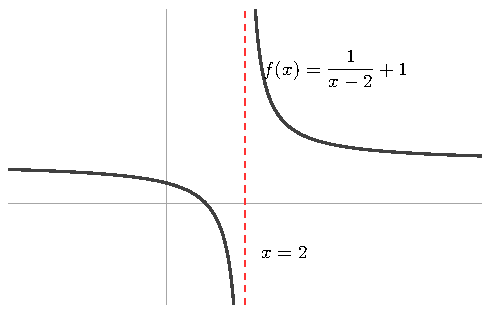
\includegraphics{figuras/asintota-vertical.pdf}
        \caption{La recta $x=2$ es una asíntota vertical de la gráfica de la función $f(x)=
        1/(x-2)+1$, pues $\lim_{x\to 2^{+}}f(x)=\infty$.}
        \label{fig:4.9}
    \end{figure}

    \subtitulo{Asíntotas Horizontales}

    Si $\lim_{x\to\infty}f(x)=L$, donde $L$ es un número real, entonces los valores $f(x)$
    se aproximarán al número $L$ si $x$ es suficientemente grande, en consecuencia,
    la gráfica de $f$ se «aproximará» a la recta $y=L$ si $x$ es suficientemente
    grande. Una situación análoga ocurre si $\lim_{x\to-\infty}f(x)=L$. Por esta razón,
    a la recta $y=L$ le damos un nombre especial.

    \begin{definicion}[Asíntota horizontal]\label{def:36}
        Sea $L$ un número real. Si $\lim_{x\to\infty}f(x)=
        L$ o $\lim_{x\to-\infty}f(x)=L$, entonces a la recta $y=L$ le llamaremos \textit{asíntota
        horizontal}\index{asintota horizontal@asíntota horizontal} de la gráfica de $f$ (véase la figura~\ref{fig:4.10}).
    \end{definicion}

    \begin{figure}[H]
        \centering
        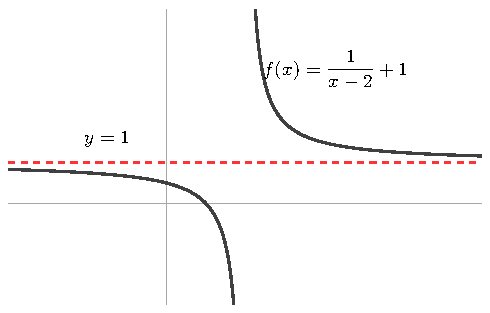
\includegraphics{figuras/asintota-horizontal.pdf}
        \caption{La recta $y=1$ es una asíntota horizontal de la gráfica de la función $f(x)=
        1/(x-2)+1$, pues $\lim_{x\to\infty}f(x)=1$.}
        \label{fig:4.10}
    \end{figure}

    \subtitulo{Asíntotas Oblicuas}

    Consideremos la recta
    \begin{equation*}
        l(x)=mx+b,\ \ m\neq 0.
    \end{equation*}
    Si $\lim_{x\to\infty}f(x)-l(x)=0$, entonces la diferencia entre los valores $f(x)$ y
    $l(x)$ se aproximarán a $0$ si $x$ es suficientemente grande, en consecuencia, la
    gráfica de $f$ se «aproximará» a la recta $y=mx+b$ si $x$ es suficientemente
    grande. Una situación análoga ocurre si $\lim_{x\to-\infty}f(x)-l(x)=0$. Por esta
    razón, a la recta $y=mx+b$ le damos un nombre especial.

    \begin{definicion}[Asíntota oblicua]\label{def:37}
        Sean $m$ y $b$ números reales con $m\neq 0$.
        Si $\lim_{x\to\infty}f(x)-(mx+b)=0$ o $\lim_{x\to-\infty}f(x)-(mx+b)=0$, entonces a
        la recta $y=mx+b$ le llamaremos \textit{asíntota oblicua}\index{asintota oblicua@asíntota oblicua} de la gráfica de $f$ (véase
        la figura~\ref{fig:4.11}).
    \end{definicion}

    \begin{figure}[H]
        \centering
        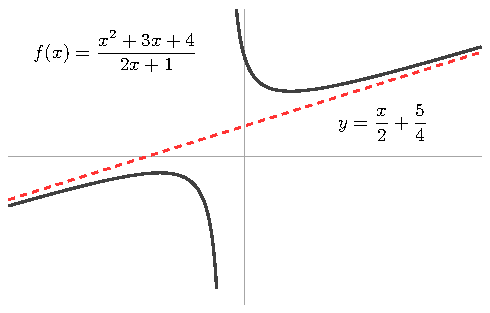
\includegraphics{figuras/asintota-oblicua.pdf}
        \caption{La recta $y=x/2+5/4$ es una asíntota oblicua de la gráfica de la función
        $f(x)=\left(x^{2}+3x+4\right)/(2x+1)$, pues $\lim_{x\to\infty}f(x)-(x/2+5/4)=0$ (¿por qué?).}
        \label{fig:4.11}
    \end{figure}

    La definición anterior no considera el caso $m=0$ simplemente por el
    significado del adjetivo «oblicua».

    \subtitulo{Curvas Asintóticas}

    Consideremos dos funciones $f$ y $g$ tales que
    \begin{equation*}
        \lim_{x\to\infty}f(x)-g(x)=0.
    \end{equation*}
    En este caso, la diferencia entre los valores $f(x)$ y $g(x)$ se aproximarán a $0$ si
    $x$ es suficientemente grande, en consecuencia, la gráfica de $f$ se «aproximará»
    a la gráfica de $g$ si $x$ es suficientemente grande. Una situación análoga ocurre
    si $\lim_{x\to-\infty}f(x)-g(x)=0$. Por esta razón, a la gráfica de $g$ le damos un
    nombre especial.

    \begin{definicion}[Curva asintótica]\label{def:38}
        Sean $f$ y $g$ funciones. Si $\lim_{x\to\infty}f(x)-
        g(x)=0$ o $\lim_{x\to-\infty}f(x)-g(x)=0$, entonces a la gráfica de $g$ le llamaremos
        \textit{curva}\footnote{En la literatura matemática, para que las gráficas de $f$ y $g$ sean llamadas «curvas» se
        suele requerir que las funciones $f$ y $g$ sean continuas. Véase la sección~\ref{sec:continuidad} para consultar
        la definición de continuidad.} \textit{asintótica}\index{curva asintotica@curva asintótica} de la gráfica de $f$, y viceversa (véase la figura~\ref{fig:4.12}).
    \end{definicion}

    \begin{figure}[H]
        \centering
        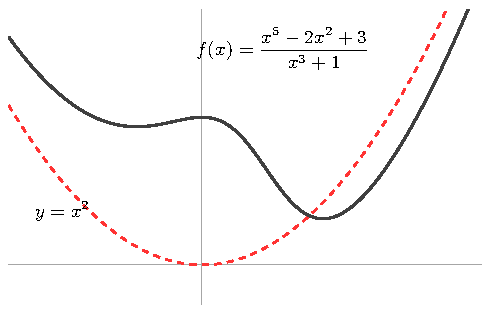
\includegraphics{figuras/curva-asintotica.pdf}
        \caption{La parábola $y=x^{2}$ es una curva asintótica de la gráfica de la función
        $f(x)=\left(x^{5}-2x^{2}+3\right)/\left(x^{3}+1\right)$, pues $\lim_{x\to\infty}f(x)-x^{2}=0$ (¿por qué?).}
        \label{fig:4.12}
    \end{figure}

    Por supuesto, el concepto de curva asintótica generaliza los conceptos de
    asíntota horizontal y de asíntota oblicua: si en la definición anterior se tiene
    que $g(x)=L$, donde $L$ es una constante, entonces la gráfica de $g$ es una
    asíntota horizontal de la gráfica de $f$; si $g(x)=mx+b$, donde $m\neq 0$,
    entonces la gráfica de $g$ es una asíntota oblicua de la gráfica de $f$.

    A continuación calcularemos las curvas asintóticas de las funciones racionales.
    Consideremos una función racional
    \begin{equation*}
        R(x)=\frac{P(x)}{Q(x)}.
    \end{equation*}
    Si el grado de $P$ es menor que el grado de $Q$, por el inciso (a) de la proposición~\ref{prop:45}
    sabemos que
    \begin{equation*}
        \lim_{x\to\pm\infty}\frac{P(x)}{Q(x)}=0.
    \end{equation*}
    En este caso la recta $y=0$ es una asíntota horizontal de la gráfica de $R$. Por
    otra parte, si el grado de $P$ es igual al grado de $Q$, por el inciso (b) de la
    proposición~\ref{prop:45} sabemos que
    \begin{equation*}
        \lim_{x\to\pm\infty}\frac{P(x)}{Q(x)}=\frac{a_{n}}{b_{n}},
    \end{equation*}
    donde $a_{n}$ y $b_{n}$ son los coeficientes principales de los polinomios $P$ y $Q$,
    respectivamente. En este caso la recta $y=a_{n}/b_{n}$ es una asíntota horizontal
    de la gráfica de $R$. Si el grado de $P$ es mayor que el grado de $Q$, al dividir
    obtenemos que
    \begin{equation*}
        \frac{P(x)}{Q(x)}=C(x)+\frac{r(x)}{Q(x)},
    \end{equation*}
    donde $C$ es un polinomio y $r$ es un polinomio de grado menor que el grado
    de $Q$. Por el inciso (a) de la proposición~\ref{prop:45} sabemos que
    \begin{equation*}
        \lim_{x\to\pm\infty}\frac{r(x)}{Q(x)}=0
    \end{equation*}
    y, en consecuencia, que
    \begin{equation*}
        \lim_{x\to\pm\infty}\frac{P(x)}{Q(x)}-C(x)=0,
    \end{equation*}
    lo cual indica que la gráfica del polinomio $C$ es una curva asintótica de la
    gráfica de $R$. Resumimos estos resultados en la proposición siguiente.

    \begin{proposicion}[Curvas asintóticas de gráficas de funciones racionales]\label{prop:55}
        Sea
        \begin{equation*}
            R(x)=\frac{P(x)}{Q(x)}
        \end{equation*}
        una función racional.
        \begin{enumerate}[nosep]
            \item Si el grado de $P$ es menor que el grado de $Q$, entonces la recta $y=0$ es
            una asíntota horizontal de la gráfica de $R$.
            \item Si el grado de $P$ es igual al grado de $Q$, entonces la recta $y=a_{n}/b_{n}$,
            donde $a_{n}$ y $b_{n}$ son los coeficientes principales de los polinomios $P$ y $Q$,
            respectivamente, es una asíntota horizontal de la gráfica de $R$.
            \item Si el grado de $P$ es mayor que el grado de $Q$, entonces la gráfica del polinomio
            $C$, donde $C(x)$ es el cociente de la división de $P(x)$ entre $Q(x)$,
            es una curva asintótica de la gráfica de $R$. En el caso particular en que el
            grado de $P$ es $n$ y el grado de $Q$ es $n-1$ se tiene que el polinomio $C$ es de
            grado $1$ y, en consecuencia, su gráfica es una recta con pendiente distinta
            de cero. En este caso la gráfica de $C$ es una asíntota oblicua de la gráfica
            de $R$.
        \end{enumerate}
    \end{proposicion}

    \begin{ejemplo}[Curva asintótica]\label{ejm:67}
        Encuentra, si las hay, las curvas asintóticas
        de la gráfica de la función
        \begin{equation*}
            f(x)=\frac{x^{5}-2x^{2}+3}{x^{3}+1}.
        \end{equation*}

        \textbf{Solución.} Notemos primero que la función $f$ es una función racional con el
        grado del numerador mayor que el grado del denominador. Al dividir obtenemos
        que
        \begin{equation*}
            \frac{x^{5}-2x^{2}+3}{x^{3}+1}=x^{2}-\frac{3x^{2}-3}{x^{3}+1}.
        \end{equation*}
        Por la proposición~\ref{prop:55} sabemos que la parábola $y=x^{2}$ es una curva asintótica
        de la gráfica de $f$ (véase la figura~\ref{fig:4.12}).
    \end{ejemplo}

    \begin{ejemplo}[Curva asintótica]\label{ejm:68}
        Encuentra, si las hay, las curvas asintóticas
        de la gráfica de la función
        \begin{equation*}
            f(x)=\frac{x^{2}}{3x+5}.
        \end{equation*}

        \textbf{Solución.} Al dividir obtenemos que
        \begin{equation*}
            \frac{x^{2}}{3x+5}=\left(\frac{1}{3}x-\frac{5}{9}\right)+\frac{25}{27x+45}.
        \end{equation*}
        Por la proposición~\ref{prop:55} sabemos que la recta $y=x/3-5/9$ es una curva
        asintótica, en realidad una asíntota oblicua, de la gráfica de $f$ (véase la figura~\ref{fig:4.11}).
    \end{ejemplo}

    \par\avoidorphan{6}\subsection*{Ejercicios}

    \begin{ejercicio}\label{ej:187}
        Encuentra las asíntotas verticales (si las hay) de las funciones
        siguientes:
        \begin{multicols}{2}
        \begin{enumerate}[nosep]
            \item $f(x)=\frac{4}{(x-2)^{3}}$.
            \item $f(x)=\frac{2+x}{x^{2}(1-x)}$.
            \item $f(x)=\frac{10x^{2}-9x}{x^{3}+1}$.
        \end{enumerate}
        \end{multicols}
    \end{ejercicio}

    \begin{ejercicio}\label{ej:188}
        Encuentra las asíntotas horizontales (si las hay) de las funciones
        siguientes:
        \begin{multicols}{2}
        \begin{enumerate}[nosep]
            \item $f(x)=\frac{1}{x^{2}+1}$.
            \item $f(x)=\frac{-2x^{3}+10x^{2}-9x-2}{x^{3}+1}$.
            \item $f(x)=\frac{3x^{2}+2x-1}{4x^{5}-3x^{3}}+5$.
        \end{enumerate}
        \end{multicols}
    \end{ejercicio}

    \begin{ejercicio}\label{ej:189}
        Encuentra las asíntotas oblicuas (si las hay) de las funciones
        siguientes:
        \begin{multicols}{2}
        \begin{enumerate}[nosep]
            \item $f(x)=\frac{2x^{2}-x+1}{3x-6}$.
            \item $f(x)=\frac{x^{3}-2x+4}{3x^{2}+1}$.
            \item $f(x)=\frac{2x^{5}-7}{x^{4}+3}$.
        \end{enumerate}
        \end{multicols}
    \end{ejercicio}

    \section{Continuidad}\label{sec:continuidad}

    Después de haber estudiado los límites de funciones y sus propiedades,
    estamos listos para introducir y estudiar en esta sección uno de los conceptos
    más importantes del cálculo, la continuidad. Iniciamos con su definición.

    \begin{definicion}[Continuidad]\label{def:39}
        Sea $f$ una función definida en un intervalo
        abierto $I$ que contiene a $p$.
        \begin{enumerate}[nosep]
            \item Diremos que $f$ es \textit{continua}\index{continuidad}\index{funcion continua@función continua} en $p$ si
            \begin{equation}\label{eq:4.42}
                \lim_{x\to p}f(x)=f(p).
            \end{equation}
            Diremos que $f$ es discontinua en $p$ si $f$ no es continua en $p$.
            \item Diremos que $f$ es \textit{continua} (en $I$) si $f$ es continua en todo punto de $I$.
            Diremos que $f$ es discontinua si $f$ no es continua.
        \end{enumerate}
    \end{definicion}

    \begin{observacion}\label{obs:18}
        Notemos lo siguiente:
        \begin{enumerate}[label=\arabic*.,nosep]
            \item Por definición, si $f$ no está definida en $p$, entonces $f$ no es continua en $p$.
            \item Según la definición de límite, \eqref{eq:4.42} se cumple si para todo $\epsilon>0$, existe
            $\delta>0$ tal que si $x\in I$ y $0<|x-p|<\delta$, entonces $|f(x)-f(p)|<\epsilon$.
            Notemos entonces que para que \eqref{eq:4.42} se cumpla no es necesario considerar
            la condición de que $0<|x-p|$, pues si $x=p$ siempre se cumple que
            $|f(x)-f(p)|<\epsilon$. Así pues, $f$ es continua en $p$ si para todo $\epsilon>0$, existe
            $\delta>0$ tal que si $x\in I$ y $|x-p|<\delta$, entonces $|f(x)-f(p)|<\epsilon$; o en
            símbolos, si
            \begin{equation}\label{eq:4.43}
                \forall\epsilon>0,\exists\delta>0,\forall x\in\R,[x\in I\wedge|x-p|<\delta]\Rightarrow|f(x)-f(p)|<\epsilon.
            \end{equation}
        \end{enumerate}
    \end{observacion}

    Como vimos anteriormente, no todas las funciones $f$ tienen la propiedad
    de que para calcular $\lim_{x\to p}f(x)$ simplemente hay que evaluar $f$ en $p$, las
    funciones continuas son precisamente las funciones que tienen esa propiedad.
    Por otra parte, ¿cuál es la razón de que a las funciones que cumplen \eqref{eq:4.42} se
    les llame continuas en $p$? El adjetivo «continua» se justifica en la observación
    siguiente.

    \begin{observacion}\label{obs:19}
        Notemos lo siguiente:
        \begin{enumerate}[label=\arabic*.,nosep]
            \item Si $f$ es continua en $p$, entonces $\lim_{x\to p}f(x)$ existe y, en consecuencia, los
            límites laterales $\lim_{x\to p^{-}}f(x)$ y $\lim_{x\to p^{+}}f(x)$ existen y son iguales. Esto
            evita que la gráfica de $f$ tenga un «salto» en $x=p$, como el «salto» que
            tiene la gráfica de la función de la figura~\ref{fig:4.13} en $x=0$.
            \item Si $f$ es continua en $p$, además de que los límites laterales $\lim_{x\to p^{-}}f(x)$
            y $\lim_{x\to p^{+}}f(x)$ existen y son iguales, son iguales a $f(p)$. Esto evita que
            la gráfica de $f$ tenga un «hueco» en $x=p$, como el «hueco» que tiene la
            gráfica de la función de la figura~\ref{fig:4.14} en $x=3$.
        \end{enumerate}
    \end{observacion}

    Así pues, si $f$ es continua en $p$, entonces la gráfica de $f$ no tiene ni «saltos»
    ni «huecos» en $x=p$, como en las gráficas de las figuras~\ref{fig:4.13} y~\ref{fig:4.14},
    respectivamente, de ahí el adjetivo «continua». Por supuesto, las funciones
    de las figuras~\ref{fig:4.13} y~\ref{fig:4.14} son ejemplos de funciones que no son continuas en
    $0$ y en $3$ respectivamente.

    \begin{figure}[H]
        \centering
        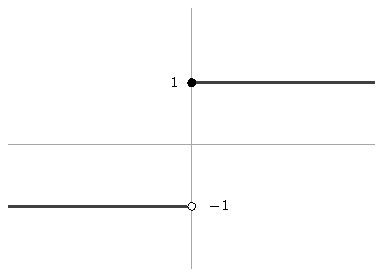
\includegraphics{figuras/escalon.pdf}
        \caption{La gráfica de la función $f(x)=\begin{cases}1, & \text{si }x\geq 0,\\ -1, & \text{si }x<0\end{cases}$ tiene un «salto» en $x=0$.}
        \label{fig:4.13}
    \end{figure}

    \begin{figure}[H]
        \centering
        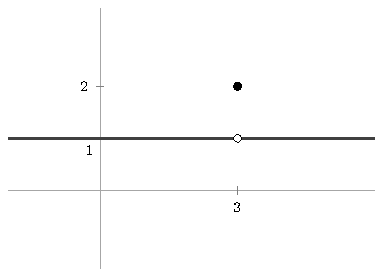
\includegraphics{figuras/funcion-salto-punto.pdf}
        \caption{La gráfica de la función $f(x)=\begin{cases}1, & \text{si }x\neq 3,\\ 2, & \text{si }x=3\end{cases}$ tiene un «hueco» o «agujero»
        en $x=3$.}
        \label{fig:4.14}
    \end{figure}

    Cabe en este momento, una vez que disponemos del concepto de continuidad,
    hacer la observación siguiente.

    \begin{observacion}[«Podemos meter o sacar el límite de una función continua»]\label{obs:20}
        En el contexto de la proposición~\ref{prop:41}, si $\lim_{x\to p}g(x)=L$ y $f$ es
        continua en $L$, entonces $\lim_{x\to p}f(g(x))=f(L)$, es decir,
        \begin{equation}\label{eq:4.44}
            \lim_{x\to p}f(g(x))=f\left(\lim_{x\to p}g(x)\right).
        \end{equation}
        En base a la ecuación \eqref{eq:4.44} podemos decir (de manera informal y en lenguaje
        usual) que
        \begin{center}
            «podemos meter o sacar el límite de una función continua».
        \end{center}
        Por ejemplo, puesto que la función valor absoluto es continua (véase el inciso
        (c) de la proposición~\ref{prop:33}), entonces
        \begin{equation*}
            \lim_{x\to p}|g(x)|=\left|\lim_{x\to p}g(x)\right|
        \end{equation*}
        para toda función $g$ cuyo límite cuando $x$ tiende a $p$ existe. En otras palabras,
        «podemos meter o sacar el límite de la función valor absoluto».
    \end{observacion}

    A continuación mostraremos varias maneras de obtener funciones continuas
    a partir de otras funciones continuas.

    De la proposición~\ref{prop:36} obtenemos el resultado siguiente.

    \begin{proposicion}[Álgebra de funciones continuas]\label{prop:56}
        \index{algebra de funciones continuas@álgebra de funciones continuas}Sean $f$ y $g$ funciones
        definidas en un intervalo abierto $I$ que contiene a $p$.
        \begin{enumerate}[nosep]
            \item Si $f$ y $g$ son continuas en $p$, entonces $f+g$, $f-g$, $fg$ y $f/g$ (si $g(p)\neq 0$)
            son continuas en $p$.
            \item Si $f$ y $g$ son continuas, entonces $f+g$, $f-g$, $fg$ y $f/g$ (si $g(x)\neq 0$ para
            todo punto $x$ de $I$) son continuas.
        \end{enumerate}
    \end{proposicion}

    Ahora nos toca hablar de la continuidad de la composición de funciones.

    \begin{proposicion}[Continuidad de la composición de funciones]\label{prop:57}
        Sean
        $g$ una función definida en un intervalo abierto $I$ que contiene a $p$ y $f$ una
        función definida en un intervalo abierto $J$ que contiene a $g(p)$. Supongamos
        que $g(I)\subset J$, de manera que la composición $f\circ g$ está definida en $I$.
        \begin{enumerate}[nosep]
            \item Si $g$ es continua en $p$ y $f$ es continua en $g(p)$, entonces $f\circ g$ es continua
            en $p$.
            \item Si $f$ y $g$ son continuas, entonces $f\circ g$ es continua.
        \end{enumerate}
    \end{proposicion}

    \begin{proof}
        El inciso (a) se sigue de la proposición~\ref{prop:41} y el inciso (b) se
        sigue de (a).
    \end{proof}

    Recordemos que una función definida en un intervalo abierto $I$ que contiene
    a $p$ es continua en $p$ si se cumple \eqref{eq:4.43}. Notemos que \eqref{eq:4.43} tiene sentido
    si $I$ no necesariamente es un intervalo abierto; tomaremos a \eqref{eq:4.43} como
    motivación para definir la continuidad de una función en dominios más generales
    y no solo en intervalos abiertos.

    \begin{definicion}[Continuidad en dominios más generales]\label{def:40}
        \index{continuidad en dominios mas generales@continuidad en dominios más generales}Sea $f$ una
        función definida en un conjunto $A$ que contiene a $p$.
        \begin{enumerate}[nosep]
            \item Diremos que $f$ es \textit{continua} en $p$ si para todo $\epsilon>0$, existe $\delta>0$ tal que
            si $x\in A$ y $|x-p|<\delta$, entonces $|f(x)-f(p)|<\epsilon$.\footnote{Recordemos que la expresión «si $x\in A$ y $|x-p|<\delta$, entonces $|f(x)-f(p)|<\epsilon$» es
            una abreviación de la proposición «$\forall x\in\R,[x\in A\wedge|x-p|<\delta]\Rightarrow|f(x)-f(p)|<\epsilon$».} Diremos que $f$ es
            discontinua en $p$ si $f$ no es continua en $p$.
            \item Diremos que $f$ es \textit{continua} (en $A$) si $f$ es continua en todo punto de $A$.
            Diremos que $f$ es discontinua si $f$ no es continua.
        \end{enumerate}
    \end{definicion}

    \begin{observacion}\label{obs:21}
        Es importante hacer las observaciones siguientes sobre la
        definición~\ref{def:40}:
        \begin{enumerate}[label=\arabic*.]
            \item Si en la definición~\ref{def:40} el conjunto $A$ es un intervalo abierto que contiene
            a $p$, entonces la definición que resulta coincide con la definición~\ref{def:39} que
            vimos previamente, es decir, la definición~\ref{def:39} es un caso particular de la
            definición~\ref{def:40}.
            \item Es sencillo mostrar (véase el ejercicio~\ref{ej:204}) que una función $f$ es continua
            en un intervalo cerrado $[a,b]$ con $a<b$ ssi $f$ es continua en el intervalo
            abierto $(a,b)$ y
            \begin{equation*}
                \lim_{x\to a^{+}}f(x)=f(a)\ \text{ y }\ \lim_{x\to b^{-}}f(x)=f(b).
            \end{equation*}
            Resultados similares se tienen para la continuidad de una función en intervalos
            de la forma $(a,b]$, $[a,b)$, $(-\infty,a]$ o $[a,\infty)$. A una función que
            cumple que $\lim_{x\to p^{+}}f(x)=f(p)$ se le llama \textit{continua por la derecha}\index{funcion continua por la derecha en un punto@función continua por la derecha en un punto} en
            $p$. De manera similar, a una función que cumple que $\lim_{x\to p^{-}}f(x)=f(p)$
            se le llama \textit{continua por la izquierda}\index{funcion continua por la izquierda en un punto@función continua por la izquierda en un punto} en $p$.
            \item Notemos que, por definición, una función que no está definida en $p$ no
            puede ser continua en $p$.
            \item Es sencillo probar (véase el ejercicio~\ref{ej:205}) que una función cuyo dominio es
            un conjunto con un solo punto es continua. Más en general, una función
            cuyo dominio es un conjunto finito es continua.
            \item Notemos que existen funciones $f$ continuas en un punto $p$, según la definición~\ref{def:40},
            que no cumplen la ecuación
            \begin{equation}\label{eq:4.45}
                \lim_{x\to p}f(x)=f(p)
            \end{equation}
            que considera la definición~\ref{def:39}. Por ejemplo, si el dominio de una función
            $f$ es el conjunto $\{p\}$, entonces $f$ es continua en $p$ según la definición~\ref{def:40}
            y, sin embargo, no se cumple \eqref{eq:4.45}; la razón de esto último es que para
            que se cumpla \eqref{eq:4.45} se requiere, por definición, que $f$ esté definida en un
            intervalo abierto que contenga a $p$ y claramente el conjunto $\{p\}$ contiene
            a $p$ y, sin embargo, no es un intervalo abierto.
        \end{enumerate}
    \end{observacion}

    Antes de continuar es importante señalar que las proposiciones~\ref{prop:56} y~\ref{prop:57}
    también se cumplen en el contexto más general de la definición~\ref{def:40}, es decir,
    tales proposiciones se cumplen cuando el dominio de las funciones consideradas
    no necesariamente es un intervalo abierto.

    Tanto los polinomios como las funciones racionales, las funciones trigonométricas,
    la función logaritmo natural, la exponencial, la función raíz $n$-ésima
    y la función valor absoluto son continuas (en su dominio) según la definición~\ref{def:40}.

    Con las proposiciones~\ref{prop:56} y~\ref{prop:57} podemos construir un buen número de
    funciones continuas. Por ejemplo, la función monstruosa
    \begin{equation*}
        \sqrt{\frac{\sqrt[7]{8x^{6}+\sin^{2}(x)}\,\ln\left(\left|1-x^{10}\right|\right)\left(11x^{3}-4x\right)}{e^{\sin\left(100\sqrt{1+x^{4}}\right)}+\frac{\cos^{4}\left(3+6x-45x^{2}\right)}{1+4x^{6}}}+\left|\frac{x^{70-x^{4}}\cos\left(x^{5}+3x^{4}-46\right)}{\sqrt[3]{\left|9x^{8}e^{x}+1\right|}+11}\right|}
    \end{equation*}
    es una función continua (en su dominio).

    Dedicaremos el resto de esta sección a probar, mediante el axioma del
    supremo, tres de los teoremas más importantes sobre continuidad, los teoremas
    de la función acotada, del mínimo y máximo, y del valor intermedio.
    Probaremos primero el teorema de la función acotada.

    \begin{teorema}[de la función acotada]\label{teo:1}
        \index{teorema de la funcion acotada@teorema de la función acotada}Si $f:[a,b]\to\R$ es continua,
        entonces $f$ es acotada.
    \end{teorema}

    \begin{proof}
        Si $a=b$, el resultado es claro. Supongamos que $a<b$ y
        consideremos el conjunto
        \begin{equation*}
            A=\{x\in[a,b]:f\text{ es acotada en }[a,x]\}.
        \end{equation*}
        Claramente $A$ es no vacío y acotado superiormente, en consecuencia, existe
        $\alpha=\sup(A)$. Probaremos que $\alpha=b$ y a partir de ahí mostraremos que $f$
        es acotada en $[a,b]$.\footnote{Notemos que para mostrar que $f$ es acotada en $[a,b]$ no basta con probar que $\alpha=b$,
        pues el supremo de un conjunto puede no pertenecer al conjunto.} Puesto que $b$ es una cota superior del conjunto $A$,
        entonces $a\leq\alpha\leq b$. Supongamos primero que $\alpha=a$. Como $f$ es continua en
        $a$, existe $\delta>0$ con $a+\delta<b$ tal que
        \begin{equation*}
            \text{si }x\in[a,b]\text{ y }|x-a|<\delta,\text{ entonces }|f(x)-f(a)|<1.
        \end{equation*}
        Así, por la desigualdad del triángulo, si $x\in[a,b]$ y $|x-a|<\delta$, entonces
        \begin{align*}
            |f(x)|&\leq|f(x)-f(a)|+|f(a)|\\
            &<1+|f(a)|.
        \end{align*}
        Esto indica que $f$ es acotada en $[a,a+\delta)$ y, en consecuencia, en $[a,a+\delta/2]$.
        Esto último señala que $a+\delta/2\in A$, lo cual contradice que $\alpha=a$ es cota
        superior de $A$; así, $a<\alpha\leq b$. Supongamos ahora que $\alpha<b$. Puesto que $f$ es
        continua en $\alpha$, existe $\delta>0$ con $a<\alpha-\delta<\alpha+\delta<b$ tal que
        \begin{equation*}
            \text{si }x\in[a,b]\text{ y }|x-\alpha|<\delta,\text{ entonces }|f(x)-f(\alpha)|<1.
        \end{equation*}
        Así, por la desigualdad del triángulo, si $x\in[a,b]$ y $|x-\alpha|<\delta$, entonces
        \begin{equation*}
            |f(x)|<1+|f(\alpha)|.
        \end{equation*}
        Esto ahora indica que $f$ es acotada en $(\alpha-\delta,\alpha+\delta)$ y, en consecuencia, en
        $[\alpha-\delta/2,\alpha+\delta/2]$. Por otra parte, por la proposición~\ref{prop:13}, sabemos que existe
        $x\in A$ tal que $\alpha-\delta/2<x\leq\alpha$, lo cual implica que $f$ es acotada en $[a,x]$
        y, en consecuencia, en $[a,\alpha-\delta/2]$. Como $f$ es acotada tanto en $[a,\alpha-\delta/2]$
        como en $[\alpha-\delta/2,\alpha+\delta/2]$, resulta que $f$ es acotada en $[a,\alpha+\delta/2]$, lo cual
        nuevamente contradice que $\alpha$ es cota superior de $A$; así, $\alpha=b$. Mostraremos
        finalmente que $f$ es acotada en $[a,b]$. Ya que $f$ es continua en $b$, como en la
        primera parte de la prueba, existe $\delta>0$ con $a<b-\delta$ tal que $f$ es acotada en
        $[b-\delta/2,b]$. Por otra parte, como $\alpha=b$, por la proposición~\ref{prop:13}, sabemos que
        existe $x\in A$ tal que $b-\delta/2<x\leq b$, lo cual implica que $f$ es acotada en $[a,x]$
        y, en consecuencia, en $[a,b-\delta/2]$. Como $f$ es acotada tanto en $[b-\delta/2,b]$
        como en $[a,b-\delta/2]$, entonces $f$ es acotada en $[a,b]$.
    \end{proof}

    Toca el turno de mostrar el teorema del mínimo y máximo. Damos primero
    la definición siguiente.

    \begin{definicion}[Valores mínimo y máximo de una función]\label{def:41}
        Sea $A$ un
        subconjunto de $\R$ y consideremos una función $f:A\to\R$.
        \begin{enumerate}
            \item Diremos que $f(p)$ es el \textit{mínimo}\index{minimo de una funcion@mínimo de una función} de $f$ (o el \textit{mínimo global}\index{minimo global de una funcion@mínimo global de una función} de $f$) si
            \begin{equation*}
                f(p)\leq f(x)\text{ para todo }x\in A.
            \end{equation*}
            En este caso se dice que el mínimo de $f$ se alcanza en $p$.
            \item Diremos que $f(p)$ es el \textit{máximo}\index{maximo de una funcion@máximo de una función} de $f$ (o el \textit{máximo global}\index{maximo global de una funcion@máximo global de una función} de $f$) si
            \begin{equation*}
                f(x)\leq f(p)\text{ para todo }x\in A.
            \end{equation*}
            En este caso se dice que el máximo de $f$ se alcanza en $p$.
        \end{enumerate}
    \end{definicion}

    Al mínimo y máximo de una función también se les llama extremos\index{extremos de una funcion@extremos de una función} de la
    función. Notemos que el mínimo (máximo) de $f$ es el mínimo (máximo) de
    su imagen $f(A)$.

    Por ejemplo, el mínimo de la función $\sin(x)$ es $-1$ y se alcanza en los
    puntos de la forma $-\pi/2+2k\pi$, con $k$ entero; por otra parte, su máximo es
    $1$ y se alcanza en los puntos de la forma $\pi/2+2k\pi$ con $k$ entero (véase la
    figura~\ref{fig:4.15}).

    No todas las funciones tienen mínimo o máximo. La figura~\ref{fig:4.16} muestra
    funciones que no tienen mínimo o máximo o ni mínimo ni máximo.

    \begin{teorema}[del mínimo y máximo]\label{teo:2}
        \index{teorema del minimo y maximo@teorema del mínimo y máximo}Si $f:[a,b]\to\R$ es continua,
        entonces $f$ tiene mínimo y máximo.
    \end{teorema}

    \begin{figure}[H]
        \centering
        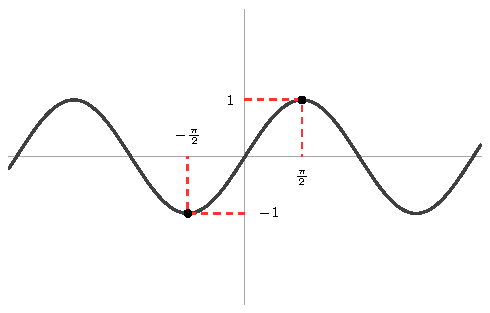
\includegraphics{figuras/seno-extremos.pdf}
        \caption{Los números $-1$ y $1$ son el mínimo y máximo de la función $\sin(x)$,
        respectivamente.}
        \label{fig:4.15}
    \end{figure}

    \begin{figure}[H]
        \centering
        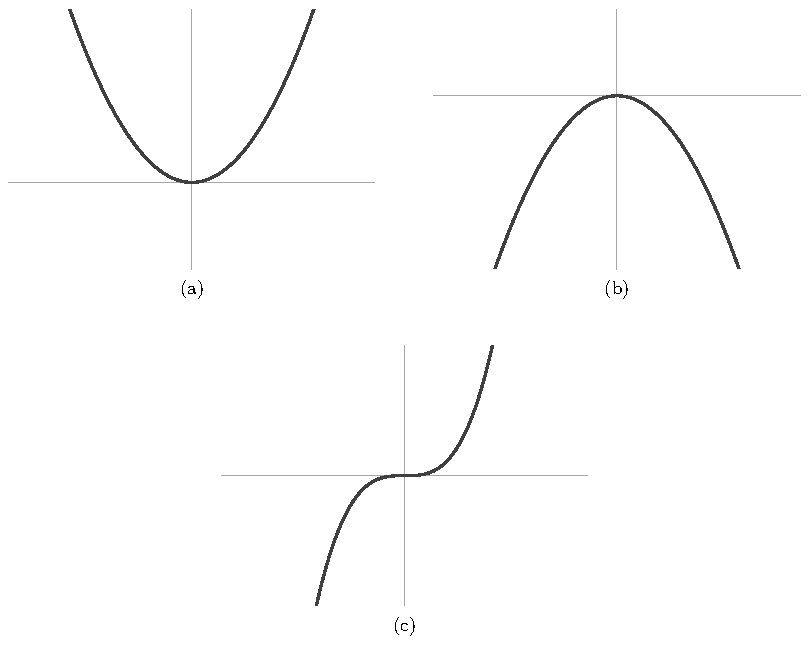
\includegraphics{figuras/sin-extremos.pdf}
        \caption{En el inciso (a) se muestra la gráfica de la función $x^{2}$, la cual tiene un
        mínimo, pero no tiene un máximo; en el inciso (b) se muestra la gráfica de la función $-x^{2}$,
        la cual tiene un máximo, pero no tiene un mínimo; en el inciso (c) se muestra la gráfica de
        la función $x^{3}$, la cual no tiene ni mínimo ni máximo.}
        \label{fig:4.16}
    \end{figure}

    \begin{proof}
        Probaremos que $f$ tiene máximo. La prueba de que $f$ tiene
        mínimo es similar. Si $a=b$, el resultado es claro. Supongamos que $a<b$ y
        consideremos el conjunto
        \begin{equation*}
            A=\{f(x):x\in[a,b]\}.
        \end{equation*}
        Como $A$ es no vacío y acotado superiormente, pues $f$ es acotada, entonces
        existe $\alpha=\sup(A)$. Probaremos que $\alpha$ es el máximo de $f$. Supongamos que
        $\alpha$ no es el máximo de $f$. En consecuencia, para todo $x\in[a,b]$ se tiene que
        $f(x)<\alpha$. Consideremos a la función $g:[a,b]\to\R$ dada por
        \begin{equation*}
            g(x)=\frac{1}{\alpha-f(x)}.
        \end{equation*}
        Puesto que $f$ es continua, entonces $g$ es continua. Por otra parte, por la
        proposición~\ref{prop:13}, para cada $M>0$, existe $x_{M}\in[a,b]$ tal que
        \begin{equation*}
            \alpha-\frac{1}{M}<f(x_{M})<\alpha.
        \end{equation*}
        Así,
        \begin{equation*}
            g(x_{M})=\frac{1}{\alpha-f(x_{M})}>M
        \end{equation*}
        y, en consecuencia, $g$ no es acotada, lo cual es una contradicción. Por lo tanto,
        $\alpha$ es el máximo de $f$.
    \end{proof}

    Como veremos en el próximo capítulo, la existencia de un mínimo o un
    máximo de una función es importante en las aplicaciones. Más adelante veremos
    un método para calcular el mínimo y el máximo de una función continua
    definida en un intervalo cerrado $[a,b]$, una vez que el teorema~\ref{teo:2} nos garantiza
    su existencia.

    El lema siguiente, importante por sí mismo, expresa una propiedad de las
    funciones continuas que usaremos para mostrar el teorema del valor intermedio.

    \begin{lema}[Lema importante]\label{lem:1}
        Sea $f:[a,b]\to\R$ con $a<b$.
        \begin{enumerate}
            \item Si $f(a)>c$ y $f$ es continua en $a$, existe $\delta>0$ tal que
            \begin{equation*}
                f(x)>c\text{ para todo }x\in[a,a+\delta).
            \end{equation*}
            \item Si $f(b)>c$ y $f$ es continua en $b$, existe $\delta>0$ tal que
            \begin{equation*}
                f(x)>c\text{ para todo }x\in(b-\delta,b].
            \end{equation*}
            \item Si $p\in(a,b)$, $f(p)>c$ y $f$ es continua en $p$, existe $\delta>0$ tal que
            \begin{equation*}
                f(x)>c\text{ para todo }x\in(p-\delta,p+\delta).
            \end{equation*}
        \end{enumerate}
        Se tienen resultados análogos si $f(a)<c$, $f(b)<c$ o si $f(p)<c$, respectivamente.
    \end{lema}

    \begin{proof}
        Probaremos el inciso (a), los incisos (b) y (c) se prueban de
        manera similar. Supongamos que $f(a)>c$ y que $f$ es continua en $a$. Por
        la continuidad de $f$ en $a$, existe $\delta>0$ con $a+\delta<b$ tal que si $x\in[a,b]$ y
        $|x-a|<\delta$, entonces
        \begin{equation*}
            |f(x)-f(a)|<f(a)-c,
        \end{equation*}
        es decir,
        \begin{equation}\label{eq:4.46}
            c-f(a)<f(x)-f(a)<f(a)-c.
        \end{equation}
        Así, si $x\in[a,a+\delta)$, por la primera desigualdad de \eqref{eq:4.46}, obtenemos que
        $f(x)>c$.
    \end{proof}

    \begin{teorema}[del valor intermedio]\label{teo:3}
        \index{teorema del valor intermedio}Si $f:[a,b]\to\R$ es continua y $c$ es
        un número con
        \begin{equation*}
            f(a)<c<f(b)\ \text{ o }\ f(b)<c<f(a),
        \end{equation*}
        entonces existe $x\in(a,b)$ tal que $f(x)=c$.
    \end{teorema}

    \begin{proof}
        Supongamos que $f(a)<c<f(b)$, el caso en que $f(b)<c<
        f(a)$ se prueba de manera similar. Sea
        \begin{equation*}
            A=\{x\in[a,b]:f(x)<c\}.
        \end{equation*}
        Como $A$ es no vacío, pues $a\in A$, y acotado superiormente, entonces existe
        $\alpha=\sup(A)$. Puesto que $b$ es cota superior del conjunto $A$, entonces $a\leq
        \alpha\leq b$. Mostraremos que $a<\alpha<b$ y que $f(\alpha)=c$, de lo cual obtendremos
        lo afirmado. Supongamos que $\alpha=a$. Como $f(a)<c$ y $f$ es continua en $a$,
        por el lema~\ref{lem:1}, existe $\delta>0$ tal que si $x\in[a,a+\delta)$, entonces $f(x)<c$, lo
        cual contradice que $\alpha=a$ es cota superior de $A$ y, en consecuencia, $a<\alpha$.
        Supongamos ahora que $\alpha=b$. Puesto que $f(b)>c$ y $f$ es continua en $b$,
        por el lema~\ref{lem:1}, existe $\delta>0$ tal que si $x\in(b-\delta,b]$, entonces $f(x)>c$.
        Por otra parte, por la proposición~\ref{prop:13}, existe $x\in A$ tal que $x\in(b-\delta,b]$.
        Así, $x\in A$ y $f(x)>c$, lo cual es una contradicción. Luego, $\alpha<b$ y, en
        consecuencia, $a<\alpha<b$. Ahora probaremos que $f(\alpha)=c$. Supongamos que
        $f(\alpha)<c$. Como $f$ es continua en $\alpha$, por el lema~\ref{lem:1}, existe $\delta>0$ tal que
        si $x\in(\alpha-\delta,\alpha+\delta)$, entonces $f(x)<c$, lo cual contradice que $\alpha$ es cota
        superior de $A$. Supongamos ahora que $f(\alpha)>c$. Puesto que $f$ es continua en
        $\alpha$, por el lema~\ref{lem:1}, existe $\delta>0$ tal que si $x\in(\alpha-\delta,\alpha+\delta)$, entonces $f(x)>c$.
        Por otra parte, por la proposición~\ref{prop:13}, existe $x\in A$ tal que $x\in(\alpha-\delta,\alpha]$.
        Así, $x\in A$ y $f(x)>c$, lo cual es una contradicción. Finalmente, como no es
        posible que $f(\alpha)<c$ o que $f(\alpha)>c$, concluimos que $f(\alpha)=c$.
    \end{proof}

    Es importante señalar que, además del axioma del supremo, la continuidad
    es una propiedad crucial para asegurar las conclusiones de los teoremas de la
    función acotada, del mínimo y máximo, y del valor intermedio.

    Como una primera consecuencia del teorema del valor intermedio (teorema~\ref{teo:3})
    obtenemos otro resultado clásico sobre continuidad.

    \begin{teorema}\label{teo:4}
        Si $f:I\to\R$ es continua e $I$ es un intervalo, entonces $f(I)$ es
        un intervalo.
    \end{teorema}

    \begin{proof}
        Si $f$ es constante, el resultado es claro. Supongamos que $f$ no
        es constante. Recordemos, del ejercicio~\ref{ej:49}, que un subconjunto $J$ de $\R$ es un
        intervalo ssi $J$ cumple la condición siguiente:
        \begin{equation*}
            \text{Para todo }p,q\in J,\ \text{si }p<c<q,\ \text{entonces }c\in J.
        \end{equation*}
        Tomemos $p,q\in f(I)$ y supongamos que $p<c<q$. Existen $x,y\in I$
        tales que $p=f(x)$ y $q=f(y)$. Sin pérdida de generalidad\footnote{Cuando en una demostración se presentan varios casos, digamos los casos (a), (b) y
        (c), y escribimos, por ejemplo, «sin pérdida de generalidad supongamos el caso (a)», nos
        referimos a que la demostración en los casos restantes es análoga.}
        supongamos que $x<y$. Puesto que $I$ es un intervalo, entonces $[x,y]\subset I$.
        Así, $f:[x,y]\to\R$ es una función continua (véase el ejercicio~\ref{ej:202}) tal que
        $f(x)<c<f(y)$. Por el teorema del valor intermedio (teorema~\ref{teo:3}), existe
        $w\in(x,y)$ tal que $f(w)=c$. Luego, $c\in f(I)$, de lo cual concluimos que
        $f(I)$ es un intervalo.
    \end{proof}

    Como otra aplicación del teorema del valor intermedio (teorema~\ref{teo:3}) veamos
    el ejemplo siguiente.

    \begin{ejemplo}[Solución de ecuaciones]\label{ejm:69}
        Como consecuencia del teorema
        del valor intermedio (teorema~\ref{teo:3}) mostraremos que la ecuación
        \begin{equation}\label{eq:4.47}
            2x^{537}+8\ln\left(1+x^{2}\right)\sin(1-x)=3(1-x)^{97}
        \end{equation}
        tiene una solución en el intervalo $[0,1]$. En efecto, sea $f(x)=2x^{537}+
        8\ln\left(1+x^{2}\right)\sin(1-x)-3(1-x)^{97}$. Puesto que
        \begin{equation*}
            f(0)=-3<0<2=f(1),
        \end{equation*}
        por el teorema del valor intermedio (teorema~\ref{teo:3}) existe $x\in(0,1)$ tal que
        $f(x)=0$, lo cual es equivalente a que $x$ sea solución de la ecuación \eqref{eq:4.47}.
    \end{ejemplo}

    \par\avoidorphan{6}\subsection*{Ejercicios}

    \begin{ejercicio}\label{ej:190}
        Da un ejemplo de una función $f:\R\to\R$ que sea continua
        solo en el punto $x=0$.
    \end{ejercicio}

    \begin{ejercicio}\label{ej:191}
        Da un ejemplo de una función $f:\R\to\R$ que sea continua
        solo en un punto $p$.
    \end{ejercicio}

    \begin{ejercicio}\label{ej:192}
        Da un ejemplo de una función $f:\R\to\R$ que sea continua
        solo en un número finito de puntos $p_{1},\ldots,p_{n}$.
    \end{ejercicio}

    \begin{ejercicio}\label{ej:193}
        Da un ejemplo de una función $f:\R\to\R$ que sea discontinua
        solo en un número finito de puntos $p_{1},\ldots,p_{n}$.
    \end{ejercicio}

    \begin{ejercicio}[Función de Dirichlet]\label{ej:194}
        \index{funcion de dirichlet@función de Dirichlet}Definimos la \textit{función de Dirichlet}
        $D:\R\to\R$ como
        \begin{equation*}
            D(x)=\begin{cases}
                1, & \text{si }x\in\Q,\\
                0, & \text{si }x\in\I.
            \end{cases}
        \end{equation*}
        \begin{enumerate}[nosep]
            \item Bosqueja la gráfica de la función de Dirichlet.
            \item Muestra que la función de Dirichlet es discontinua en todo número real.
        \end{enumerate}
    \end{ejercicio}

    \begin{ejercicio}[Función de Thomae]\label{ej:195}
        \index{funcion de thomae@función de Thomae}Definimos la \textit{función de Thomae}
        $T:\R\to\R$ como
        \begin{equation*}
            T(x)=\begin{cases}
                0 & \text{si }x\in\I,\\
                1/q, & \text{si }x=p/q\text{ es una fracción}\\
                & \text{irreducible con }p\in\Z\text{ y }q\in\N.
            \end{cases}
        \end{equation*}
        \begin{enumerate}[nosep]
            \item Muestra que la función de Thomae es periódica, de periodo $1$, es decir,
            que $T(x)=T(x+1)$, $x\in\R$.
            \item Bosqueja la gráfica de la restricción de la función de Thomae al intervalo
            $[0,1]$ (usa un programa de computadora o consulta su gráfica en internet).
            \item Muestra que la función de Thomae es continua en todo número irracional
            y discontinua en todo número racional. En cursos más avanzados de
            matemáticas como Análisis Matemático o Topología se suele probar que
            no existe una función continua en todo número racional y discontinua en
            todo número irracional.
        \end{enumerate}
    \end{ejercicio}

    \begin{ejercicio}\label{ej:196}
        Considera la función
        \begin{equation*}
            f(x)=\begin{cases}
                \sin(1/x), & \text{si }x\neq 0,\\
                0, & \text{si }x=0.
            \end{cases}
        \end{equation*}
        La gráfica de $f$ aparece en la figura~\ref{fig:3.13}. Muestra que $f$ es continua en todo
        $\R$, excepto en $0$.
    \end{ejercicio}

    \begin{ejercicio}\label{ej:197}
        Considera la función
        \begin{equation*}
            f(x)=\begin{cases}
                x\sin(1/x), & \text{si }x\neq 0,\\
                0, & \text{si }x=0.
            \end{cases}
        \end{equation*}
        La gráfica de $f$ aparece en la figura~\ref{fig:3.14}. Muestra que $f$ es continua. \sugerencia
        Para probar que $f$ es continua en $0$ usa que $|\sin(x)|\leq 1$ para toda
        $x$.
    \end{ejercicio}

    \begin{ejercicio}\label{ej:198}
        Considera la función
        \begin{equation*}
            f(x)=\begin{cases}
                x^{2}\sin(1/x), & \text{si }x\neq 0,\\
                0, & \text{si }x=0.
            \end{cases}
        \end{equation*}
        La gráfica de $f$ aparece en la figura~\ref{fig:3.15}. Muestra que $f$ es continua. \sugerencia
        Para probar que $f$ es continua en $0$ usa que $|\sin(x)|\leq 1$ para toda
        $x$.
    \end{ejercicio}

    \begin{ejercicio}\label{ej:199}
        Sean $f$ y $g$ funciones continuas en un intervalo $I$. ¿Son
        continuas las funciones $\min\{f,g\}$ y $\max\{f,g\}$? Argumenta tu respuesta.
    \end{ejercicio}

    \begin{ejercicio}\label{ej:200}
        Sea $f:\R\to\R$ una función continua. Prueba que si $f(x)=0$
        para todo número racional $x$, entonces $f=0$. \sugerencia Procede por
        contradicción y considera el lema~\ref{lem:1}.
    \end{ejercicio}

    \begin{ejercicio}\label{ej:201}
        Sean $f,g:\R\to\R$ funciones continuas. Prueba que si $f(x)=
        g(x)$ para todo número racional $x$, entonces $f=g$.
    \end{ejercicio}

    \begin{ejercicio}\label{ej:202}
        Prueba que si $f:B\to\R$ es continua y $A\subset B$, entonces
        $f|_{A}:A\to\R$ es continua.
    \end{ejercicio}

    \begin{ejercicio}\label{ej:203}
        Realiza lo siguiente:
        \begin{enumerate}[nosep]
            \item Prueba que si $f$ es continua en un intervalo cerrado $I$ y $f$ es continua en
            un intervalo cerrado $J$, entonces $f$ es continua en $I\cup J$.
            \item Proporciona un ejemplo de una función $f$ tal que $f$ es continua en un
            intervalo $I$, $f$ es continua en un intervalo $J$ y $f$ no es continua en $I\cup J$.
        \end{enumerate}
    \end{ejercicio}

    \begin{ejercicio}\label{ej:204}
        Muestra que una función $f$ es continua en un intervalo cerrado
        $[a,b]$ con $a<b$ ssi $f$ es continua en el intervalo abierto $(a,b)$ y
        \begin{equation*}
            \lim_{x\to a^{+}}f(x)=f(a)\ \text{ y }\ \lim_{x\to b^{-}}f(x)=f(b).
        \end{equation*}
        Resultados similares se tienen para la continuidad de una función en intervalos
        de la forma $(a,b]$, $[a,b)$, $(-\infty,a]$ o $[a,\infty)$. A una función que cumple
        que $\lim_{x\to p^{+}}f(x)=f(p)$ se le llama \textit{continua por la derecha}\index{funcion continua por la derecha en un punto@función continua por la derecha en un punto} en $p$. De
        manera similar, a una función que cumple que $\lim_{x\to p^{-}}f(x)=f(p)$ se le llama
        \textit{continua por la izquierda}\index{funcion continua por la izquierda en un punto@función continua por la izquierda en un punto} en $p$.
    \end{ejercicio}

    \begin{ejercicio}\label{ej:205}
        Prueba que una función cuyo dominio es un conjunto con un
        solo punto es continua. Más en general, prueba que una función cuyo dominio
        es un conjunto finito $\{p_{1},\ldots,p_{n}\}$ es continua.
    \end{ejercicio}

    \begin{ejercicio}\label{ej:206}
        Considera una función $f:[a,b]\to\R$.
        \begin{enumerate}[nosep]
            \item Prueba que si $f$ es creciente (monótona creciente) en $(a,b)$ y $f$ es continua
            en $a$, entonces $f$ es creciente (monótona creciente) en $[a,b)$.
            \item Prueba que si $f$ es creciente (monótona creciente) en $(a,b)$ y $f$ es continua
            en $b$, entonces $f$ es creciente (monótona creciente) en $(a,b]$.
            \item Prueba que si $f$ es creciente (monótona creciente) en $(a,b)$ y $f$ es continua
            en $a$ y en $b$ entonces $f$ es creciente (monótona creciente) en $[a,b]$.
        \end{enumerate}
        Un resultado similar se cumple para funciones decrecientes (monótonas decrecientes)
        en $(a,b)$. \sugerencia Para probar el inciso (a) supón primero
        que $f$ es creciente en $(a,b)$. En este caso basta mostrar que si $a<x<b$,
        entonces $f(a)<f(x)$. Supón que $a<x<b$ toma un punto $p$ tal que
        $a<p<x$. Como $f$ es creciente en $(a,b)$, entonces $f(x)-f(p)>0$. Puesto
        que $f$ es continua en $a$, existe $\delta>0$ tal que si $y\in[a,b]$ y $|y-a|<\delta$, entonces
        $|f(y)-f(a)|<f(x)-f(p)$. Al tomar $y$ tal que $a<y<p$ y $|y-a|<\delta$ se
        tiene entonces que $|f(y)-f(a)|<f(x)-f(p)$, de lo cual resulta que
        \begin{align*}
            f(a)&<f(y)+f(x)-f(p)\\
            &<f(p)+f(x)-f(p) &&\text{(pues $y<p$)}\\
            &=f(x).
        \end{align*}
        Supón ahora que $f$ es monótona creciente en $(a,b)$. En este caso basta mostrar
        que si $a<x<b$, entonces $f(a)\leq f(x)$. Supón que $a<x<b$ y
        considera los casos siguientes:
        \begin{description}[nosep,font=\normalfont]
            \item[Caso 1:] Para toda $p\in(a,x)$ se tiene que $f(p)=f(x)$.
            \item[Caso 2:] Existe $p\in(a,x)$ tal que $f(p)<f(x)$.
        \end{description}
        Prueba, usando la continuidad de $f$ en $a$, que en cualquiera de los casos
        anteriores se tiene que $f(a)\leq f(x)$. La prueba del inciso (b) es similar a la
        del inciso (a) y la prueba del inciso (c) se sigue de los incisos (a) y (b).
    \end{ejercicio}

    \begin{ejercicio}[Desigualdades de funciones II]\label{ej:207}
        Sean $f$ y $g$ dos funciones
        definidas en un subconjunto $A$ de $\R$ y definamos $h(x)=f(x)-g(x)$, $x\in A$.
        Prueba lo siguiente:
        \begin{enumerate}[nosep]
            \item Si $h$ tiene un mínimo no negativo, entonces $g(x)\leq f(x)$, $x\in A$.
            \item Si $h$ tiene un máximo no positivo, entonces $f(x)\leq g(x)$, $x\in A$.
        \end{enumerate}
        Por supuesto, las desigualdades entre las funciones $f$ y $g$ de los incisos anteriores
        pueden ser estrictas en algunos casos, por ejemplo, si en el inciso (a) se
        tiene que el mínimo de $h$ es positivo, entonces $g(x)<f(x)$, $x\in A$. No enunciamos
        estos casos buscando la simplicidad en el enunciado. Este resultado,
        aunque sencillo, será de gran utilidad para mostrar desigualdades de funciones,
        sobre todo una vez que dispongamos de herramientas para encontrar el
        mínimo y máximo de una función en la sección~\ref{sec:aplicaciones-derivada}.
    \end{ejercicio}

    \begin{ejercicio}\label{ej:208}
        Muestra que la ecuación $x^{7}+3x^{5}-x-2=0$ tiene una
        solución en el intervalo $[0,1]$.
    \end{ejercicio}

    \begin{ejercicio}\label{ej:209}
        Muestra que la ecuación $x^{5}\cos^{1000}(\pi x/2)+4x-3=0$ tiene
        una solución en el intervalo $[0,1]$.
    \end{ejercicio}

    \begin{ejercicio}\label{ej:210}
        Muestra que el rango de un polinomio de grado impar es todo
        $\R$. \sugerencia Trata de aplicar el teorema del valor intermedio (teorema~\ref{teo:3}).
    \end{ejercicio}

    \begin{ejercicio}\label{ej:211}
        Sea $f:[0,1]\to[0,1]$. Prueba que si $f$ es continua, entonces
        existe $p\in[0,1]$ tal que
        \begin{equation*}
            f(p)=p.
        \end{equation*}
        En este caso a $p$ se le llama un punto fijo de $f$. \sugerencia Nota que
        encontrar un punto $p$ tal que $f(p)=p$ es equivalente a encontrar un punto
        $p$ tal que $g(p)=0$, donde $g(x)=f(x)-x$. Intenta aplicar el teorema del
        valor intermedio (teorema~\ref{teo:3}).
    \end{ejercicio}

    \begin{ejercicio}\label{ej:212}
        Sea $f:\R\to\R$. Prueba que si $f$ es continua y $f(\R)\subset\Q$,
        entonces $f$ es una función constante. \sugerencia Considera el teorema~\ref{teo:4}.
    \end{ejercicio}

    \begin{ejercicio}[Las funciones continuas mandan intervalos cerrados y acotados en intervalos cerrados y acotados]\label{ej:213}
        Prueba que si $f$ es continua
        en $[a,b]$, entonces $f([a,b])=[m,M]$, donde $m=\min\{f(x):x\in[a,b]\}$
        y $M=\max\{f(x):x\in[a,b]\}$.
    \end{ejercicio}

    \begin{ejercicio}[Las funciones continuas y 1-1 en un intervalo son crecientes o decrecientes en el intervalo]\label{ej:214}
        Prueba que si $f$ es continua
        y 1-1 en un intervalo $I$, entonces $f$ es creciente o $f$ es decreciente en $I$.
        \sugerencia Supón que el intervalo $I$ es de la forma $[a,b]$ con $a<b$, la
        prueba en los otros casos la dejamos a tu cargo. Como $f$ es 1-1, entonces
        $f(a)\neq f(b)$. Si, por ejemplo, $f(a)<f(b)$ prueba, usando el teorema del
        valor intermedio (teorema~\ref{teo:3}), que $f(a)<f(x)<f(b)$ para todo $a<x<b$
        y de ahí muestra que $f$ es creciente en $I$.
    \end{ejercicio}

    \begin{ejercicio}[Las funciones continuas y 1-1 mandan intervalos abiertos en intervalos abiertos]\label{ej:215}
        Prueba que si $f$ es continua y 1-1 en
        un intervalo abierto $I$, entonces $f(I)$ es un intervalo abierto. \sugerencia
        Por el ejercicio~\ref{ej:214} sabemos que $f$ es creciente o decreciente. Supón que $f$ es
        creciente, la prueba en el caso en que $f$ es decreciente es similar. Expresa
        \begin{equation*}
            I=\bigcup_{n=1}^{\infty}[a_{n},b_{n}],
        \end{equation*}
        con $a_{n+1}<a_{n}<b_{n}<b_{n+1}$. Como $f$ es creciente, entonces
        \begin{equation*}
            f(I)=f\left(\bigcup_{n=1}^{\infty}[a_{n},b_{n}]\right)=\bigcup_{n=1}^{\infty}f([a_{n},b_{n}])=\bigcup_{n=1}^{\infty}[f(a_{n}),f(b_{n})].
        \end{equation*}
        Finalmente, prueba que
        \begin{equation*}
            f(I)=\left(\inf_{n\in\N}f(a_{n}),\sup_{n\in\N}f(b_{n})\right).
        \end{equation*}
    \end{ejercicio}

    \section{Discontinuidades}

    Para que una función $f$ definida en un intervalo abierto $I$ que contiene a
    $p$ sea continua en $p$ se debe satisfacer que
    \begin{equation*}
        \lim_{x\to p}f(x)=f(p).
    \end{equation*}
    Existen varias maneras en que esto deja de cumplirse. Esto motiva a la
    definición siguiente.

    \begin{definicion}[Discontinuidades esenciales, de salto y removibles]\label{def:42}
        Sea $f$ una función definida en un intervalo abierto $I$ que contiene a $p$.
        \begin{enumerate}[nosep]
            \item Diremos que $f$ tiene una \textit{discontinuidad esencial}\index{discontinuidad esencial} en $p$ si $\lim_{x\to p^{+}}f(x)$ o
            $\lim_{x\to p^{-}}f(x)$ no existen.
            \item Diremos que $f$ tiene una \textit{discontinuidad de salto}\index{discontinuidad de salto} en $p$ si $\lim_{x\to p^{+}}f(x)$ y
            $\lim_{x\to p^{-}}f(x)$ existen, pero son diferentes.
            \item Diremos que $f$ tiene una \textit{discontinuidad removible}\index{discontinuidad removible} en $p$ si $\lim_{x\to p}f(x)$
            existe, pero es distinto de $f(p)$.
        \end{enumerate}
    \end{definicion}

    Por supuesto, el nombre de discontinuidad removible del inciso (c) de la
    definición anterior proviene del hecho de que podemos redefinir la función $f$
    en $p$ (¿cómo?) de manera que la función resultante sea continua en $p$. Notemos
    que si $f$ tiene una discontinuidad esencial o una discontinuidad de salto en
    $p$, entonces no podemos redefinir $f$ en $p$ de manera que la función resultante
    sea continua en $p$.

    Si denotamos por $D$ al conjunto de discontinuidades de $f$ y por $E$, $S$ y
    $R$ a los conjuntos de sus discontinuidades esenciales, de salto y removibles,
    respectivamente, entonces es claro que
    \begin{equation*}
        D=E\cup S\cup R
    \end{equation*}
    y que esta unión es ajena.

    Por ejemplo, consideremos a la función
    \begin{equation*}
        f(x)=\begin{cases}
            \sin(1/x), & \text{si }x\neq 0,\\
            0, & \text{si }x=0.
        \end{cases}
    \end{equation*}
    Como $\lim_{x\to 0^{-}}f(x)$ no existe (véase la figura~\ref{fig:3.13} y el ejercicio~\ref{ej:158}), entonces
    $f$ tiene una discontinuidad esencial en $0$. Por otra parte, la función de la figura~\ref{fig:4.13}
    tiene una discontinuidad de salto en $x=0$ y la función de la figura~\ref{fig:4.14}
    tiene una discontinuidad removible en $x=3$.

    La proposición siguiente muestra que, en caso de existir, las discontinuidades
    de una función monótona siempre son de salto.

    \begin{proposicion}[Funciones monótonas y sus discontinuidades]\label{prop:58}
        Sea
        $f$ una función definida en un intervalo abierto $(a,b)$ que contiene a $p$. Se
        cumple lo siguiente:
        \begin{enumerate}
            \item Si $f$ es monótona creciente, entonces
            \begin{equation}\label{eq:4.48}
                \lim_{x\to p^{-}}f(x)=\sup_{a<x<p}f(x)\leq f(p)\leq\inf_{p<x<b}f(x)=\lim_{x\to p^{+}}f(x).
            \end{equation}
            \item Si $f$ es monótona decreciente, entonces
            \begin{equation}\label{eq:4.49}
                \lim_{x\to p^{-}}f(x)=\inf_{a<x<p}f(x)\geq f(p)\geq\sup_{p<x<b}f(x)=\lim_{x\to p^{+}}f(x).
            \end{equation}
            \item Si $f$ es monótona y tiene una discontinuidad en $p$, entonces la discontinuidad
            de $f$ en $p$ es de salto.
        \end{enumerate}
    \end{proposicion}

    \begin{proof}
        (a) Puesto que $f$ es monótona creciente es claro que se
        cumplen las dos desigualdades de \eqref{eq:4.48}. Sea $\epsilon>0$ y definamos $L_{1}=
        \sup\{f(x):a<x<p\}$ y $L_{2}=\inf\{f(x):p<x<b\}$. Por la proposición~\ref{prop:13},
        existe $a<x_{0}<p$ tal que
        \begin{equation*}
            L_{1}-\epsilon<f(x_{0})\leq L_{1}.
        \end{equation*}
        Sea $\delta=p-x_{0}>0$. Luego, si $0<p-x<\delta$, entonces $x_{0}<x<p$ y, en
        consecuencia, como $f$ es monótona creciente,
        \begin{equation*}
            L_{1}-\epsilon<f(x_{0})\leq f(x)\leq L_{1},
        \end{equation*}
        de lo cual resulta que $|f(x)-L_{1}|<\epsilon$. Hemos probado así que $\lim_{x\to p^{-}}f(x)=
        L_{1}$. De manera similar se prueba que $\lim_{x\to p^{+}}f(x)=L_{2}$.

        (b) La demostración de esta afirmación es similar a la demostración del
        inciso (a).

        (c) Supongamos que $f$ es monótona creciente y que $f$ tiene una discontinuidad
        en $p$. El resultado se sigue de \eqref{eq:4.48}, en efecto, en la prueba de
        \eqref{eq:4.48} mostramos que $\lim_{x\to p^{-}}f(x)$ y $\lim_{x\to p^{+}}f(x)$ existen, así que la
        discontinuidad de $f$ en $p$ no es esencial. La discontinuidad de $f$ en $p$ tampoco
        es removible, pues si lo fuera de \eqref{eq:4.48} obtendríamos que $f$ es continua en
        $p$, lo cual sería una contradicción. Por lo tanto, la discontinuidad de $f$ en $p$
        es de salto. De manera similar, la prueba en el caso en que $f$ es monótona
        decreciente se sigue de \eqref{eq:4.49}.
    \end{proof}

    \par\avoidorphan{6}\subsection*{Ejercicios}

    \begin{ejercicio}\label{ej:216}
        Sea
        \begin{equation*}
            f(x)=\begin{cases}
                x^{2}, & \text{si }x\neq 2,\\
                5, & \text{si }x=2.
            \end{cases}
        \end{equation*}
        \begin{enumerate}[nosep]
            \item Dibuja la gráfica de $f$.
            \item Calcula, si existen, $\lim_{x\to 2^{-}}f(x)$ y $\lim_{x\to 2^{+}}f(x)$.
            \item Determina si existe $\lim_{x\to 2}f(x)$ (argumenta tu respuesta). En caso afirmativo
            calcúlalo.
            \item Determina si $f$ es continua en $2$. Argumenta tu respuesta.
            \item Si $f$ no es continua en $2$, determina si la discontinuidad en $2$ es esencial,
            de salto o removible.
            \item Si $f$ no es continua en $2$, ¿puedes redefinir $f$ en $2$ para que lo sea? Argumenta
            tu respuesta.
        \end{enumerate}
    \end{ejercicio}

    \begin{ejercicio}\label{ej:217}
        Sea
        \begin{equation*}
            f(x)=\frac{x^{3}-6x+9}{x-1}.
        \end{equation*}
        \begin{enumerate}[nosep]
            \item Dibuja la gráfica de $f$.
            \item Calcula, si existen, $\lim_{x\to 1^{-}}f(x)$ y $\lim_{x\to 1^{+}}f(x)$.
            \item Determina si existe $\lim_{x\to 1}f(x)$ (argumenta tu respuesta). En caso afirmativo
            calcúlalo.
            \item Determina si $f$ es continua en $1$. Argumenta tu respuesta.
            \item Si $f$ no es continua en $1$, determina si la discontinuidad en $1$ es esencial,
            de salto o removible.
            \item Si $f$ no es continua en $1$, ¿puedes redefinir $f$ en $1$ para que lo sea? Argumenta
            tu respuesta.
        \end{enumerate}
    \end{ejercicio}

    \begin{ejercicio}\label{ej:218}
        Sea
        \begin{equation*}
            f(x)=\begin{cases}
                x^{2}+1, & \text{si }x\geq 0,\\
                x, & \text{si }x<0.
            \end{cases}
        \end{equation*}
        \begin{enumerate}[nosep]
            \item Dibuja la gráfica de $f$.
            \item Calcula, si existen, $\lim_{x\to 0^{-}}f(x)$ y $\lim_{x\to 0^{+}}f(x)$.
            \item Determina si existe $\lim_{x\to 0}f(x)$ (argumenta tu respuesta). En caso afirmativo
            calcúlalo.
            \item Determina si $f$ es continua en $0$. Argumenta tu respuesta.
            \item Si $f$ no es continua en $0$, determina si la discontinuidad en $0$ es esencial,
            de salto o removible.
            \item Si $f$ no es continua en $0$, ¿puedes redefinir $f$ en $0$ para que lo sea? Argumenta
            tu respuesta.
        \end{enumerate}
    \end{ejercicio}

    \begin{ejercicio}\label{ej:219}
        Sea
        \begin{equation*}
            f(x)=\begin{cases}
                1/x, & \text{si }x\neq 0,\\
                0, & \text{si }x=0.
            \end{cases}
        \end{equation*}
        \begin{enumerate}[nosep]
            \item Dibuja la gráfica de $f$.
            \item Calcula, si existen, $\lim_{x\to 0^{-}}f(x)$ y $\lim_{x\to 0^{+}}f(x)$.
            \item Determina si existe $\lim_{x\to 0}f(x)$ (argumenta tu respuesta). En caso afirmativo
            calcúlalo.
            \item Determina si $f$ es continua en $0$. Argumenta tu respuesta.
            \item Si $f$ no es continua en $0$, determina si la discontinuidad en $0$ es esencial,
            de salto o removible.
            \item Si $f$ no es continua en $0$, ¿puedes redefinir $f$ en $0$ para que lo sea? Argumenta
            tu respuesta.
        \end{enumerate}
    \end{ejercicio}

    \begin{ejercicio}[La inversa de una función continua definida en un intervalo es una función continua]\label{ej:220}
        Sea $f$ una función definida en un
        intervalo $I$. Prueba que si $f$ es continua y 1-1, entonces $f^{-1}$ es continua.
        \sugerencia Sea $g=f^{-1}$. Supón que $I$ es un intervalo abierto, la prueba en
        los otros casos la dejamos a tu cargo. Como $f$ es continua e $I$ es un intervalo
        abierto, por el ejercicio~\ref{ej:215} sabemos que $f(I)$ es un intervalo abierto, digamos
        $(\alpha,\beta)$. Por el ejercicio~\ref{ej:214} sabemos que $f$ es creciente o decreciente. Supón
        que $f$ es creciente, la prueba en el caso en que $f$ es decreciente es similar. Por
        el ejercicio~\ref{ej:124} se tiene entonces que $g:(\alpha,\beta)\to I$ es creciente. Supón que
        $g$ tiene una discontinuidad en $y_{0}\in(\alpha,\beta)$. Por el inciso (c) de la proposición~\ref{prop:58}\footnote{Aquí es donde se usa que $I$ es un intervalo abierto, pues en este caso $f(I)$ también es
        un intervalo abierto.}
        se tiene que la discontinuidad de $g$ en $y_{0}$ es de salto, por lo cual
        \begin{equation}\label{eq:4.50}
            \lim_{y\to y_{0}^{-}}g(y)<\lim_{y\to y_{0}^{+}}g(y).
        \end{equation}
        Por el inciso (a) de la proposición~\ref{prop:58} también sabemos que
        \begin{equation}\label{eq:4.51}
            \lim_{y\to y_{0}^{-}}g(y)=\sup_{\alpha<y<y_{0}}g(y)\leq g(y_{0})\leq\inf_{y_{0}<y<\beta}g(y)=\lim_{y\to y_{0}^{+}}g(y).
        \end{equation}
        De \eqref{eq:4.50} y \eqref{eq:4.51} podemos tomar $w$ tal que
        \begin{equation*}
            \lim_{y\to y_{0}^{-}}g(y)<w<\lim_{y\to y_{0}^{+}}g(y)
        \end{equation*}
        y $w\notin g(\alpha,\beta)=I$. Por otra parte, nuevamente por \eqref{eq:4.51}, existen $\alpha<y_{1}<
        y_{0}$ y $y_{0}<y_{2}<\beta$ tales que
        \begin{equation*}
            g(y_{1})\leq\lim_{y\to y_{0}^{-}}g(y)<w<\lim_{y\to y_{0}^{+}}g(y)\leq g(y_{2}),
        \end{equation*}
        lo cual contradice que $I$ es un intervalo. Por lo tanto, $g$ es continua.
    \end{ejercicio}

    \begin{ejercicio}[Una función continua con inversa discontinua]\label{ej:221}
        Considera la función $f:[0,1]\cup(2,3]\to[0,2]$ dada por
        \begin{equation*}
            f(x)=\begin{cases}
                x, & \text{si }0\leq x\leq 1,\\
                x-1, & \text{si }2<x\leq 3.
            \end{cases}
        \end{equation*}
        Realiza lo siguiente:
        \begin{enumerate}[nosep]
            \item Dibuja la gráfica de $f$.
            \item Muestra que $f$ es continua.
            \item Encuentra la regla de correspondencia de $f^{-1}$.
            \item Dibuja la gráfica de $f^{-1}$.
            \item Muestra que $f^{-1}$ es discontinua en $1$.
        \end{enumerate}
    \end{ejercicio}

    \section{Continuidad Uniforme}

    En esta sección estudiaremos un tipo de continuidad más fuerte que el
    definido en la sección~\ref{sec:continuidad}, la continuidad uniforme. Recordemos de la
    definición~\ref{def:40} que una función $f$ definida en un conjunto $A$ que contiene a $p$ es
    continua en $p$ si para todo $\epsilon>0$, existe $\delta>0$ tal que si $x\in A$ y $|x-p|<\delta$,
    entonces $|f(x)-f(p)|<\epsilon$. En esta definición la $\delta$ depende de $\epsilon$ y del punto
    $p$ dado. Cuando, dado $\epsilon>0$, la $\delta$ no dependa del punto $p$ diremos que $f$
    es uniformemente continua en $A$. Más precisamente, tenemos la definición
    siguiente.

    \begin{definicion}[Continuidad uniforme]\label{def:43}
        \index{continuidad uniforme}\index{funcion uniformemente continua@función uniformemente continua}Sea $f$ una función definida en un
        conjunto $A$. Diremos que $f$ es \textit{uniformemente continua} (en $A$) si para todo
        $\epsilon>0$, existe $\delta>0$ tal que si $x,y\in A$ y $|x-y|<\delta$, entonces $|f(x)-f(y)|<
        \epsilon$.\footnote{Aquí a frase «si $x,y\in A$ y $|x-y|<\delta$, entonces $|f(x)-f(y)|<\epsilon$» es una abreviación
        de la proposición $\forall x\in\R,\forall y\in\R,[x\in A\wedge y\in A\wedge|x-y|<\delta]\Rightarrow|f(x)-f(y)|<\epsilon$.
        Así, en símbolos, $f$ es uniformemente continua (en $A$) si $\forall\epsilon>0,\exists\delta>0,\forall x\in
        \R,\forall y\in\R,[x\in A\wedge y\in A\wedge|x-y|<\delta]\Rightarrow|f(x)-f(y)|<\epsilon$.}
    \end{definicion}

    Claramente, una función uniformemente continua es una función continua.
    Por otra parte, una función continua no necesariamente es uniformemente
    continua, por ejemplo, la función $f(x)=x^{2}$ es continua en $\R$ y no es
    uniformemente continua en $\R$ (véase el ejercicio~\ref{ej:224}).

    A continuación mostraremos otro de los resultados clásicos sobre continuidad,
    a saber, que toda función continua definida en un intervalo $[a,b]$ es
    uniformemente continua. Para ello necesitaremos el lema siguiente.\footnote{Según el lema~\ref{lem:2}, si el intervalo $[a,b]$ cumple \eqref{eq:4.52}, entonces cumple \eqref{eq:4.53}. A esta
    propiedad de los intervalos $[a,b]$ se le llama compacidad. Para un estudio de la compacidad
    en un contexto más general véase, por ejemplo, \cite{nunez2020analisis}.}

    \begin{lema}\label{lem:2}
        Sea $A$ un conjunto no vacío. Si $\{I_{\alpha}:\alpha\in A\}$ es una colección de
        intervalos abiertos tal que
        \begin{equation}\label{eq:4.52}
            [a,b]\subset\bigcup_{\alpha\in A}I_{\alpha},
        \end{equation}
        entonces existen $\alpha_{1},\ldots,\alpha_{n}\in A$ tales que
        \begin{equation}\label{eq:4.53}
            [a,b]\subset I_{\alpha_{1}}\cup\cdots\cup I_{\alpha_{n}}.
        \end{equation}
    \end{lema}

    \begin{proof}
        En esta demostración haremos uso del axioma del supremo.
        Consideremos el conjunto $B$ de todos los $x\in[a,b]$ tales que
        \begin{equation*}
            [a,x]\subset I_{\alpha_{1}}\cup\cdots\cup I_{\alpha_{m}}
        \end{equation*}
        para algunos $\alpha_{1},\ldots,\alpha_{m}\in A$. Notemos que $B$ es no vacío y acotado
        superiormente y, en consecuencia, existe $s=\sup(B)$. Mostraremos que $s=b$ y
        que $s\in B$, con lo cual demostraremos el lema. Claramente $a\leq s\leq b$
        y, en consecuencia, por \eqref{eq:4.52}, existe $\alpha_{0}\in A$ tal que $s\in I_{\alpha_{0}}$; digamos que
        $I_{\alpha_{0}}=(p,q)$. Por la proposición~\ref{prop:13}, existe $x_{0}\in B$ tal que $p<x_{0}\leq s$. Como
        $x_{0}\in B$, existen $\alpha_{1},\ldots,\alpha_{m}\in A$ tales que
        \begin{equation}\label{eq:4.54}
            [a,x_{0}]\subset I_{\alpha_{1}}\cup\cdots\cup I_{\alpha_{m}}.
        \end{equation}
        Si suponemos que $s<b$, entonces podemos tomar $s<r<\min\{q,b\}$ y, en
        consecuencia, $[x_{0},r]\subset I_{\alpha_{0}}$. Puesto que
        \begin{equation*}
            [a,r]=[a,x_{0}]\cup[x_{0},r]\subset I_{\alpha_{1}}\cup\cdots\cup I_{\alpha_{m}}\cup I_{\alpha_{0}},
        \end{equation*}
        entonces $r\in B$, lo cual contradice que $s$ es cota superior de $B$. Por lo tanto,
        $s=b$. Resta mostrar que $s\in B$. Como $x_{0},s\in I_{\alpha_{0}}$, entonces $[x_{0},s]\subset I_{\alpha_{0}}$. En
        consecuencia, por \eqref{eq:4.54},
        \begin{equation*}
            [a,s]=[a,x_{0}]\cup[x_{0},s]\subset I_{\alpha_{1}}\cup\cdots\cup I_{\alpha_{m}}\cup I_{\alpha_{0}},
        \end{equation*}
        y, por lo tanto, $s\in B$.
    \end{proof}

    \begin{teorema}[Continuidad uniforme]\label{teo:5}
        Si $f:[a,b]\to\R$ es continua,
        entonces $f$ es uniformemente continua.
    \end{teorema}

    \begin{proof}
        Sea $\epsilon>0$. Como $f$ es continua, para cada $y\in[a,b]$, existe
        $\delta_{y}>0$ tal que si $x\in[a,b]$ y $|x-y|<\delta_{y}$, entonces $|f(x)-f(y)|<\epsilon/2$. Para
        cada $y\in[a,b]$ definamos
        \begin{equation*}
            I_{y}=(y-\delta_{y}/2,y+\delta_{y}/2).
        \end{equation*}
        Notemos que
        \begin{equation*}
            [a,b]\subset\bigcup_{y\in[a,b]}I_{y}.
        \end{equation*}
        Por el lema anterior sabemos que existen $y_{1},\ldots,y_{n}\in[a,b]$ tales que
        \begin{equation}\label{eq:4.55}
            [a,b]\subset I_{y_{1}}\cup\cdots\cup I_{y_{n}}.
        \end{equation}
        Sea $\delta=\min\{\delta_{y_{1}},\ldots,\delta_{y_{n}}\}/2>0$. Tomemos $x,y\in[a,b]$ tales que $|x-y|<\delta$.
        Por \eqref{eq:4.55} se tiene que $y\in I_{y_{i}}$ para algún $1\leq i\leq n$. Puesto que $|x-y|<\delta$,
        entonces
        \begin{align*}
            |x-y_{i}|&\leq|x-y|+|y-y_{i}|\\
            &<\delta+\frac{\delta_{y_{i}}}{2}\\
            &\leq\frac{\delta_{y_{i}}}{2}+\frac{\delta_{y_{i}}}{2}\\
            &=\delta_{y_{i}}.
        \end{align*}
        En consecuencia,
        \begin{align*}
            |f(x)-f(y)|&\leq|f(x)-f(y_{i})|+|f(y_{i})-f(y)|\\
            &<\frac{\epsilon}{2}+\frac{\epsilon}{2}\\
            &=\epsilon.
        \end{align*}
        Por lo tanto, $f$ es uniformemente continua en $[a,b]$.
    \end{proof}

    \par\avoidorphan{6}\subsection*{Ejercicios}

    \begin{ejercicio}\label{ej:222}
        Prueba que si una función es uniformemente continua,
        entonces es continua.
    \end{ejercicio}

    \begin{ejercicio}\label{ej:223}
        Prueba que la función $f(x)=x$ es uniformemente continua.
    \end{ejercicio}

    \begin{ejercicio}\label{ej:224}
        Prueba que la función $f(x)=x^{2}$ no es uniformemente
        continua.
    \end{ejercicio}

    \begin{ejercicio}\label{ej:225}
        ¿Es la función $f(x)=1/x$ uniformemente continua?
        Argumenta tu respuesta.
    \end{ejercicio}

    \begin{ejercicio}\label{ej:226}
        ¿Es la función $f(x)=\sqrt{x}$ uniformemente continua?
        Argumenta tu respuesta.
    \end{ejercicio}

    \begin{ejercicio}\label{ej:227}
        Sean $f$ y $g$ funciones definidas en un conjunto $A$. Prueba o
        da un contraejemplo a las afirmaciones siguientes:
        \begin{enumerate}[nosep]
            \item Si $f$ y $g$ son uniformemente continuas, entonces $f+g$ es uniformemente
            continua.
            \item Si $f$ y $g$ son uniformemente continuas, entonces $f-g$ es uniformemente
            continua.
            \item Si $f$ y $g$ son uniformemente continuas, entonces $fg$ es uniformemente
            continua.
            \item Si $f$ y $g$ son uniformemente continuas, entonces $f/g$ es uniformemente
            continua.
        \end{enumerate}
    \end{ejercicio}

    \begin{ejercicio}\label{ej:228}
        Prueba que si $f:B\to C$ y $g:A\to B$ son funciones uniformemente
        continuas, entonces $f\circ g:A\to C$ es uniformemente continua.
    \end{ejercicio}

    \begin{ejercicio}\label{ej:229}
        Prueba que si $f$ es una función uniformemente continua en
        un conjunto acotado $A$, entonces $f$ es acotada en $A$.
    \end{ejercicio}

    \chapter{La Derivada}\label{cap:derivada}

    Al fin iniciaremos el estudio de la derivada de una función. El contenido
    de los capítulos anteriores nos servirá como andamiaje para tal estudio. En
    el transcurso del capítulo veremos como la derivada es una herramienta muy
    poderosa sobre todo en las aplicaciones. Entre otras cosas veremos como
    la derivada nos permite definir y estudiar la velocidad de un objeto, tema
    fundamental en la física, y veremos como la derivada nos permite optimizar
    y analizar procesos de diversa índole.

    ¡Comencemos!

    \section{Definición e Interpretación de la Derivada}

    \begin{definicion}[Derivada de una función]\label{def:44}
        Sea $f$ una función definida en
        un intervalo abierto $I$ que contiene a $x$. Definimos la \textit{derivada}\index{derivada de una funcion@derivada de una función} de $f$ en $x$ como
        \begin{equation}\label{eq:5.1}
            f'(x)=\lim_{h\to 0}\frac{f(x+h)-f(x)}{h},
        \end{equation}
        si el límite existe. Si $f'(x)$ existe diremos que $f$ es \textit{derivable}\index{funcion derivable@función derivable} o \textit{diferenciable}\index{funcion diferenciable@función diferenciable} en
        $x$, y si $f$ es derivable en cada $x$ de $I$ diremos que $f$ es \textit{derivable o diferenciable}
        en $I$.\footnote{En ocasiones, como en el teorema~\ref{teo:6} y en el ejercicio~\ref{ej:233}, es necesario considerar
        funciones derivables en intervalos que no son abiertos: Se dice que una función $f$ es \textit{derivable}
        en un intervalo cerrado $[a,b]$ con $a<b$ si $f$ es derivable en el intervalo abierto $(a,b)$ y si
        $f'(a)$ y $f'(b)$ existen como límites laterales. De manera similar se define la diferenciabilidad
        de una función en intervalos de la forma $[a,b)$, $(a,b]$, $[a,\infty)$ y $(-\infty,b]$.} La función $f$ induce entonces la función $f'$ cuyo dominio es el conjunto
        de todos los $x$ tales que $f'(x)$ existe. Notemos entonces que $\dom(f')\subset
        \dom(f)$. A la función $f'$ le llamaremos la \textit{derivada} de $f$.
    \end{definicion}

    Otras notaciones para la derivada $f'(x)$ son
    \begin{equation*}
        \frac{df}{dx}(x),\ \ \frac{df(x)}{dx},\ \ \frac{d}{dx}f(x),\ \ (f(x))'\ \ \text{y}\ \ \dot{f}(x).
    \end{equation*}
    Algunas veces, para evitar confusiones, usaremos paréntesis y escribiremos,
    por ejemplo, $\frac{d(f(x))}{dx}$ y $\frac{d}{dx}(f(x))$ en lugar de $\frac{df(x)}{dx}$ y $\frac{d}{dx}f(x)$, respectivamente.
    Como sabemos, es común que la regla de correspondencia de una función
    $f$ esté dada mediante una ecuación, en este caso, en las expresiones $\frac{d(f(x))}{dx}$,
    $\frac{d}{dx}(f(x))$ y $(f(x))'$ algunas veces sustituiremos a $f(x)$ por la expresión
    algebraica que la define, por ejemplo, si $f(x)=x^{2}$, escribiremos $\frac{d\left(x^{2}\right)}{dx}$, $\frac{d}{dx}\left(x^{2}\right)$
    y $\left(x^{2}\right)'$ en lugar de $\frac{d(f(x))}{dx}$, $\frac{d}{dx}(f(x))$ y $(f(x))'$, respectivamente.\footnote{También usaremos los símbolos $\sin'(x)$, $\cos'(x)$, etc., para denotar a la derivada de
    las funciones trigonométricas, los símbolos $\arcsin'(x)$, $\arccos'(x)$, etc., para denotar a la
    derivada de las funciones trigonométricas inversas y el símbolo $\ln'(x)$ para denotar a la
    derivada de la función logaritmo natural.}

    Antes de continuar, surge la pregunta siguiente: ¿qué significa o representa
    la derivada de una función?

    \subtitulo{Interpretación Geométrica de la Derivada}

    Consideremos una función $f$ definida en un intervalo abierto $I$ que contiene
    a $x$ (véase la figura~\ref{fig:5.1}). Por simplicidad tomaremos $h>0$, la situación en
    el caso en que $h<0$ es similar. Consideremos la recta $l_{h}$ que pasa por los
    puntos $(x,f(x))$ y $(x+h,f(x+h))$. La pendiente de la recta $l_{h}$ es
    \begin{equation*}
        m(l_{h})=\frac{f(x+h)-f(x)}{h}.
    \end{equation*}
    Notemos que el cociente anterior es el cociente que aparece en la definición de
    $f'(x)$. Si $f'(x)$ existe, es decir, si el límite \eqref{eq:5.1} existe, y hacemos $h$ cada vez
    más pequeño, entonces las pendientes de las rectas $l_{h}$ se irán aproximando al
    número $f'(x)$. Esta situación nos motiva a dar la definición siguiente.

    \begin{definicion}[Recta tangente a la gráfica de una función]\label{def:45}
        Sea $f$
        una función derivable en $x$. Definimos la \textit{recta tangente a la gráfica de $f$
        en el punto} $(x,f(x))$\index{recta tangente a la grafica de una funcion en un punto@recta tangente a la gráfica de una función en un punto} como la recta que pasa por el punto $(x,f(x))$ y tiene
        pendiente $f'(x)$.
    \end{definicion}

    Con esta definición, la interpretación geométrica\index{interpretacion geometrica de la derivada@interpretación geométrica de la derivada} de la derivada es la
    siguiente:

    \cuadroresumen{7.5cm}{Interpretación Geométrica de la Derivada}{La derivada $f'(x)$ es la pendiente de la recta
    tangente a la gráfica de $f$ en el punto $(x,f(x))$.}

    \begin{figure}[H]
        \centering
        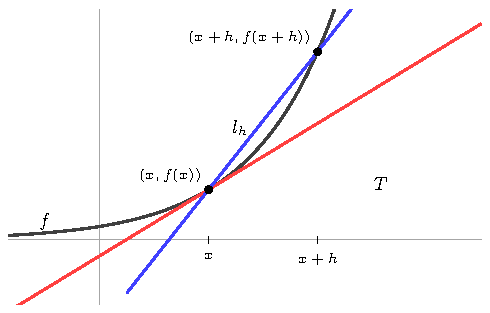
\includegraphics{figuras/derivada-geometrica.pdf}
        \caption{Interpretación geométrica de la derivada. La recta $T$ tiene pendiente $f'(x)$.}
        \label{fig:5.1}
    \end{figure}

    Más adelante, después de que hayamos visto como calcular derivadas en la
    sección~\ref{sec:calculo-derivadas}, veremos ejemplos de la interpretación geométrica de la derivada.

    \subtitulo{Interpretación Física de la Derivada}

    Supongamos que un objeto, por ejemplo, un automóvil, se mueve en línea
    recta desde un punto $A$ hasta un punto $B$ y que la distancia entre $A$ y $B$ es
    de $200$ km (véase la figura~\ref{fig:5.2}). Si el objeto tarda $2$ horas en llegar desde el
    punto $A$ hasta el punto $B$, entonces según la fórmula de la \textit{velocidad media}\index{velocidad media}
    que aprendimos en nuestras clases de física elemental,
    \begin{equation*}
        v_{m}=\frac{\text{posición final}-\text{posición inicial}}{\text{tiempo transcurrido}},
    \end{equation*}
    la velocidad media del objeto durante todo el trayecto es de $100$ km/h. Como
    su nombre lo indica, la velocidad media es un promedio y no nos da información
    de como se comportó el objeto en un instante dado $t$. Sea $s(t)$ la función
    de posición del objeto en el tiempo $t$. Por simplicidad tomaremos $h>0$, la
    situación en el caso en que $h<0$ es similar. Si $h>0$, entonces la velocidad
    media del objeto en el intervalo de tiempo $[t,t+h]$ es
    \begin{equation*}
        v_{m}(h)=\frac{s(t+h)-s(t)}{h}.
    \end{equation*}
    Intuitivamente, si $[t,t+h]$ es un intervalo de tiempo pequeño (digamos $3$
    segundos), entonces la velocidad media del objeto en ese intervalo dará una
    mejor descripción del comportamiento del objeto en el instante $t$ que la velocidad
    media del objeto durante todo el trayecto. Si hacemos $h$ cada vez
    más pequeño, entonces la velocidad media del objeto en el intervalo $[t,t+h]$
    proporcionará cada vez una mejor descripción del comportamiento del objeto
    en el instante $t$. Es natural dar entonces la definición siguiente.

    \begin{definicion}[Velocidad]\label{def:46}
        Sea $s(t)$ la función de posición de un objeto que
        se mueve en línea recta en el instante $t$. Definimos la \textit{velocidad}\index{velocidad} (o \textit{velocidad
        instantánea}\index{velocidad instantanea@velocidad instantánea}) del objeto en el instante $t$, denotada por $v(t)$, como el límite
        cuando $h$ tiende a $0$ de las velocidades medias $v_{m}(h)$ del objeto en el intervalo
        de tiempo $[t,t+h]$, en símbolos,
        \begin{equation*}
            v(t)=\lim_{h\to 0}v_{m}(h)=\lim_{h\to 0}\frac{s(t+h)-s(t)}{h}.
        \end{equation*}
        Definimos la \textit{rapidez}\index{rapidez} $r(t)$ del objeto en el instante $t$ como $|v(t)|$.
    \end{definicion}

    Si la distancia está en metros y el tiempo en segundos, las unidades de
    la velocidad son m/s; si la distancia está en km y el tiempo en horas, las
    unidades de la velocidad son km/h, etc. Las unidades de la rapidez son las
    mismas que las de la velocidad.

    Puesto que
    \begin{equation*}
        v(t)=\lim_{h\to 0}\frac{s(t+h)-s(t)}{h}=s'(t),
    \end{equation*}
    entonces la interpretación física\index{interpretacion fisica de la derivada@interpretación física de la derivada} de la derivada es la siguiente:

    \cuadroresumen{9cm}{Interpretación Física de la Derivada}{La derivada de la función de posición de un objeto que
    se mueve en línea recta $s(t)$ es la velocidad del objeto
    en el instante $t$, en símbolos, $s'(t)=v(t)$.}

    Más adelante, después de que hayamos visto como calcular derivadas en
    la sección~\ref{sec:calculo-derivadas}, veremos ejemplos de la interpretación física de la derivada.

    \begin{figure}[H]
        \centering
        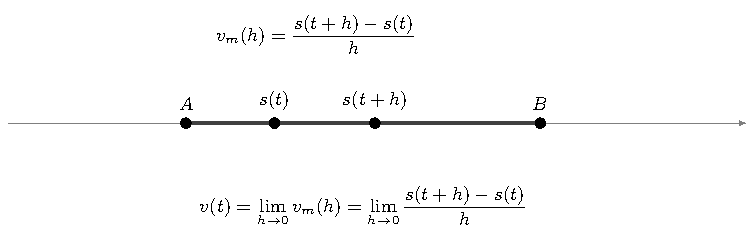
\includegraphics{figuras/derivada-fisica.pdf}
        \caption{Interpretación física de la derivada. La derivada de la función de posición de
        un objeto que se mueve en línea recta $s(t)$ es la velocidad del objeto en el instante $t$, es
        decir, $s'(t)=v(t)$.}
        \label{fig:5.2}
    \end{figure}

    \par\avoidorphan{6}\subsection*{Ejercicios}

    \begin{ejercicio}\label{ej:230}
        Sea $f$ una función definida en un intervalo abierto que
        contiene a $x$. Prueba que si una función $f$ es derivable en $x$, entonces
        \begin{equation*}
            \lim_{h\to 0}\left|\frac{f(x+h)-f(x)-hf'(x)}{h}\right|=0.
        \end{equation*}
        Recíprocamente, prueba que si existe un número real $L$ tal que
        \begin{equation*}
            \lim_{h\to 0}\left|\frac{f(x+h)-f(x)-hL}{h}\right|=0,
        \end{equation*}
        entonces $f$ es derivable en $x$ y $f'(x)=L$. \sugerencia Ten presente los
        ejercicios~\ref{ej:145} y~\ref{ej:146}.
    \end{ejercicio}

    \begin{ejercicio}\label{ej:231}
        Sea $f$ una función derivable en $x$. Prueba que
        \begin{equation*}
            f'(x)=\lim_{t\to x}\frac{f(t)-f(x)}{t-x}.
        \end{equation*}
        \sugerencia Ten presente el ejercicio~\ref{ej:147}.
    \end{ejercicio}

    \section{La Derivada como Razón de Cambio}

    En la sección pasada vimos que si $s(t)$ es la función de posición de un
    objeto que se mueve en línea recta, entonces la velocidad media del objeto
    en el intervalo de tiempo $[t_{0},t_{0}+h]$ es el cociente
    \begin{equation}\label{eq:5.2}
        \frac{s(t_{0}+h)-s(t_{0})}{h},
    \end{equation}
    y que la velocidad del objeto en el instante $t_{0}$ es el límite
    \begin{equation}\label{eq:5.3}
        \lim_{h\to 0}\frac{s(t_{0}+h)-s(t_{0})}{h}.
    \end{equation}
    El cociente \eqref{eq:5.2} nos da una medida de como cambia la función de posición
    del objeto $s(t)$ respecto del tiempo $t$ en el intervalo $[t_{0},t_{0}+h]$. Por otra
    parte, interpretamos al límite \eqref{eq:5.3} como el cambio de la función de posición
    $s(t)$ respecto del tiempo $t$ en un instante $t_{0}$. Al igual que con la función de
    posición del objeto, podemos considerar el cociente \eqref{eq:5.2} y el límite \eqref{eq:5.3} con
    otras funciones que representen propiedades físicas del objeto y que dependen
    del tiempo $t$, por ejemplo, la temperatura $T(t)$, el volumen $V(t)$, etc. Más en
    general, podemos considerar al cociente \eqref{eq:5.2} y al límite \eqref{eq:5.3} con cualquier
    función $f(x)$, donde la $x$ es una variable arbitraria y no necesariamente el
    tiempo. Estos comentarios conducen a la definición siguiente.

    \begin{definicion}[Razón de cambio media y razón de cambio]\label{def:47}
        Sea $f$
        una función definida en un intervalo abierto que contiene a $x_{0}$.
        \begin{enumerate}
            \item Definimos la \textit{razón de cambio media}\index{razon de cambio media@razón de cambio media} de la función $f$ respecto a la variable
            $x$ en el intervalo $[x_{0},x_{0}+h]$ como el cociente
            \begin{equation*}
                \frac{f(x_{0}+h)-f(x_{0})}{h}.
            \end{equation*}
            A la razón de cambio media de una función también se le llama \textit{tasa de
            cambio media}\index{tasa de cambio media} o \textit{intensidad de cambio media}\index{intensidad de cambio media}.
            \item Definimos la \textit{razón de cambio}\index{razon de cambio@razón de cambio} de la función $f$ respecto a la variable $x$ en
            el punto $x_{0}$ como el límite
            \begin{equation*}
                \lim_{h\to 0}\frac{f(x_{0}+h)-f(x_{0})}{h}.
            \end{equation*}
            En otras palabras, la razón de cambio de la función $f$ respecto a la variable
            $x$ en el punto $x_{0}$ es simplemente $f'(x_{0})$. A la razón de cambio de una
            función también se le llama \textit{tasa de cambio}\index{tasa de cambio} o \textit{intensidad de cambio}\index{intensidad de cambio}.
        \end{enumerate}
    \end{definicion}

    Para terminar esta sección definiremos la aceleración de un objeto que se
    mueve en línea recta.

    \begin{definicion}[Aceleración]\label{def:48}
        Sea $s(t)$ la función de posición de un objeto
        que se mueve en línea recta en el instante $t$. Definimos la \textit{aceleración}\index{aceleracion@aceleración} del
        objeto en el instante $t$, denotada por $a(t)$, como la razón de cambio de la
        velocidad $v(t)$ respecto al tiempo en el instante $t$, es decir,
        \begin{equation*}
            a(t)=\lim_{h\to 0}\frac{v(t+h)-v(t)}{h}=v'(t).
        \end{equation*}
    \end{definicion}

    Si la distancia está en metros y el tiempo en segundos, las unidades de
    la aceleración son m/s$^{2}$; si la distancia está en km y el tiempo en horas, las
    unidades de la aceleración son km/h$^{2}$, etc.

    En el cuadro siguiente, a manera de resumen, expresamos las fórmulas de
    la velocidad, rapidez y aceleración de un objeto que se mueve en línea recta
    con función de posición $s(t)$.
    \begin{center}
        \renewcommand{\arraystretch}{1.35}
        \begin{tabular}{|c|c|c|}
            \hline
            \textbf{Nombre} & \textbf{Símbolo} & \textbf{Fórmula}\\ \hline\noalign{\vskip 3pt}\hline
            Velocidad & $v(t)$ & $v(t)=s'(t)$\\ \hline
            Rapidez & $r(t)$ & $r(t)=|v(t)|$\\ \hline
            Aceleración & $a(t)$ & $a(t)=v'(t)$\\ \hline
        \end{tabular}
    \end{center}

    Más adelante, después de que hayamos visto como calcular derivadas en
    la sección~\ref{sec:calculo-derivadas}, veremos ejemplos del cálculo de la aceleración.

    \section{Derivabilidad y Continuidad}

    Como veremos en esta pequeña sección, para que una función sea derivable
    en un punto, tiene que ser continua en ese punto.

    \begin{proposicion}[Derivabilidad implica continuidad]\label{prop:59}
        Si $f$ es una función
        derivable en $p$, entonces $f$ es continua en $p$.
    \end{proposicion}

    \begin{proof}
        Sabemos que la continuidad de $f$ en $p$ es equivalente a que
        \begin{equation*}
            \lim_{h\to 0}f(p+h)-f(p)=0
        \end{equation*}
        (véase el ejercicio~\ref{ej:147}). Puesto que $f$ es derivable en $p$, entonces
        \begin{align*}
            \lim_{h\to 0}f(p+h)-f(p)&=\lim_{h\to 0}\left[\frac{f(p+h)-f(p)}{h}\right]h\\
            &=\lim_{h\to 0}\left[\frac{f(p+h)-f(p)}{h}\right]\cdot\lim_{h\to 0}h\\
            &=f'(p)\cdot 0\\
            &=0,
        \end{align*}
        así, $f$ es continua en $p$.
    \end{proof}

    \begin{observacion}\label{obs:22}
        Por la proposición anterior, si $f$ no es continua en $p$,
        entonces $f$ no es derivable en $p$. Así, si la gráfica de una función tiene un «salto»
        o tiene un «hueco» en $x=p$, como en las gráficas de la figura~\ref{fig:5.3}, entonces
        $f$ no es derivable en $p$.
    \end{observacion}

    \begin{figure}[H]
        \centering
        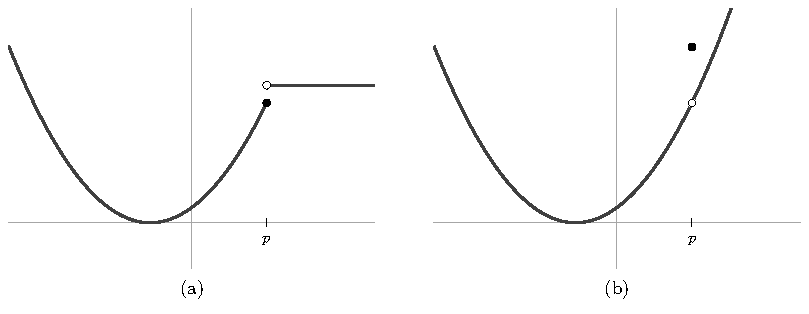
\includegraphics{figuras/no-derivable-salto.pdf}
        \caption{Si la gráfica de $f$ tiene un «salto» o un «hueco» en $x=p$, entonces $f$ no es
        derivable en $p$.}
        \label{fig:5.3}
    \end{figure}

    El recíproco de la proposición~\ref{prop:59} no es cierto, es decir, no es cierto que si
    una función es continua en $p$, entonces es derivable en $p$, como lo muestra el
    ejemplo siguiente.

    \begin{ejemplo}[La función $|x|$ es continua en $0$ y no es derivable en $0$]\label{ejm:70}
        Ya sabemos que la función $f(x)=|x|$ es continua en $0$, su gráfica se
        muestra en la figura~\ref{fig:5.4}. Para mostrar que $f$ no es derivable en cero hay
        que mostrar que $f'(0)$ no existe, para lo cual mostraremos que los límites
        laterales asociados con el límite que define a $f'(0)$ son diferentes. En efecto,
        \begin{align*}
            \lim_{h\to 0^{-}}\frac{f(0+h)-f(0)}{h}&=\lim_{h\to 0^{-}}\frac{|h|}{h}\\
            &=\lim_{h\to 0^{-}}\frac{-h}{h}\\
            &=\lim_{h\to 0^{-}}-1\\
            &=-1
        \end{align*}
        y
        \begin{align*}
            \lim_{h\to 0^{+}}\frac{f(0+h)-f(0)}{h}&=\lim_{h\to 0^{+}}\frac{|h|}{h}\\
            &=\lim_{h\to 0^{+}}\frac{h}{h}\\
            &=\lim_{h\to 0^{+}}1\\
            &=1.
        \end{align*}
        Por lo tanto, $|x|$ no es derivable en $0$.\footnote{La función valor absoluto si es derivable en los puntos distintos de cero. De hecho,
        \begin{equation*}
            (|x|)'=\begin{cases}
                1, & \text{si }x>0,\\
                -1, & \text{si }x<0,\\
                \text{no existe} & \text{si }x=0.
            \end{cases}
        \end{equation*}}
    \end{ejemplo}

    \begin{ejemplo}[Otra función continua y no derivable]\label{ejm:71}
        Consideremos la
        función $f$ definida como
        \begin{equation*}
            f(x)=\begin{cases}
                -x^{2}+3, & \text{si }x\leq 1,\\
                (x-2)^{3}+3 & \text{si }x>1.
            \end{cases}
        \end{equation*}
        Véase la figura~\ref{fig:5.5}. No es difícil mostrar que $f$ es continua y que
        \begin{equation*}
            \lim_{h\to 0^{-}}\frac{f(1+h)-f(1)}{h}=-2\neq 3=\lim_{h\to 0^{+}}\frac{f(1+h)-f(1)}{h}.
        \end{equation*}
        En consecuencia, $f$ es continua en $1$ y no derivable en $1$.
    \end{ejemplo}

    \begin{observacion}\label{obs:23}
        Si $f$ es una función derivable en $p$, entonces
        \begin{equation*}
            f'(p)=\lim_{h\to 0}\frac{f(p+h)-f(p)}{h}
        \end{equation*}
        existe y, en consecuencia, los límites laterales $\lim_{h\to 0^{-}}(f(p+h)-f(p))/h$ y
        $\lim_{h\to 0^{+}}(f(p+h)-f(p))/h$ existen y son iguales. Esto evita que la gráfica
        de $f$ tenga un «pico» en el punto $(p,f(p))$, como el «pico» que tiene la
        gráfica de la función $|x|$ en el punto $(0,f(0))$ o como el «pico» que tiene la
        gráfica de la función del ejemplo~\ref{ejm:71} en el punto $(1,f(1))$.
    \end{observacion}

    Reuniendo las observaciones~\ref{obs:22} y~\ref{obs:23} podemos decir, de manera informal,
    que si la gráfica de una función $f$ tiene un «salto» o un «hueco» en $x=p$ o
    tiene un «pico» en el punto $(p,f(p))$, entonces $f$ no es derivable en $p$ (véase
    la figura~\ref{fig:5.6}). Por supuesto, en cada caso se tendrán que mostrar de manera
    rigurosa estas afirmaciones.

    Para finalizar esta sección nos podemos preguntar, ¿si $f$ es una función
    derivable en $p$, es $f'$ continua en $p$? La respuesta es que no siempre, por
    ejemplo, en el ejercicio~\ref{ej:259} veremos (después de que sepamos como calcular
    derivadas) una función derivable (en $0$) con derivada no continua (en $0$).

    \begin{figure}[H]
        \centering
        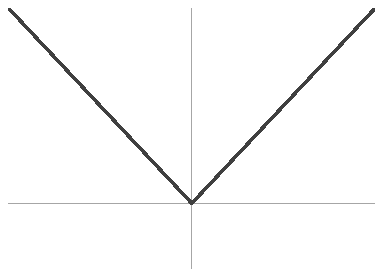
\includegraphics{figuras/valor-absoluto.pdf}
        \caption{La gráfica de la función $|x|$ tiene un «pico» en el punto $(0,f(0))$ y no es
        derivable en $0$.}
        \label{fig:5.4}
    \end{figure}

    \begin{figure}[H]
        \centering
        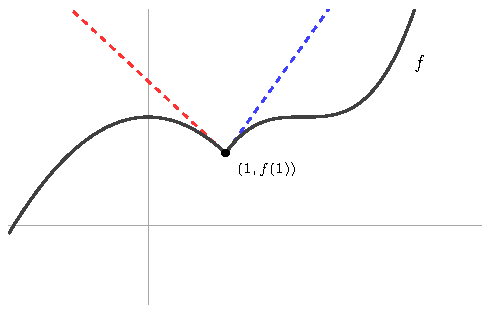
\includegraphics{figuras/pico-ejemplo.pdf}
        \caption{La gráfica de la función $f$ tiene un «pico» en el punto $(1,f(1))$ y no es
        derivable en $1$. El número $\lim_{h\to 0^{-}}(f(1+h)-f(1))/h=-2$ es la pendiente de la línea
        punteada roja y el número $\lim_{h\to 0^{+}}(f(1+h)-f(1))/h=3$ es la pendiente de la línea
        punteada azul. Si $f$ fuera diferenciable en $1$, las pendientes de las líneas punteadas roja y
        azul deberían coincidir, lo cual no sucede, en consecuencia, $f$ no es diferenciable en $1$.}
        \label{fig:5.5}
    \end{figure}

    \begin{figure}[H]
        \centering
        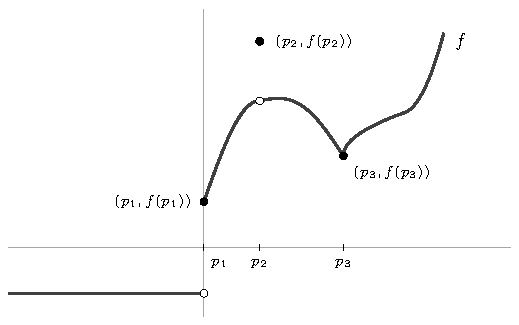
\includegraphics{figuras/no-derivable-varios.pdf}
        \caption{La función $f$ no es derivable en $p_{1}$, $p_{2}$ y $p_{3}$.}
        \label{fig:5.6}
    \end{figure}

    \par\avoidorphan{6}\subsection*{Ejercicios}

    \begin{ejercicio}\label{ej:232}
        Sean $f$ y $g$ funciones derivables en un intervalo abierto $I$. ¿Son
        derivables las funciones $\min\{f,g\}$ y $\max\{f,g\}$? Argumenta tu respuesta.
    \end{ejercicio}

    \begin{ejercicio}\label{ej:233}
        Prueba que si $f$ es una función derivable en un intervalo $[a,b]$,
        entonces $f$ es continua en $[a,b]$. \sugerencia Recuerda que una función $f$
        es derivable en un intervalo cerrado $[a,b]$ con $a<b$ si $f$ es derivable en el
        intervalo abierto $(a,b)$ y si $f'(a)$ y $f'(b)$ existen como límites laterales; ten
        presente, además, el ejercicio~\ref{ej:204}.
    \end{ejercicio}

    \section{Cálculo de Derivadas}\label{sec:calculo-derivadas}

    Ahora toca el turno del cálculo de derivadas. Calcularemos primero algunas
    derivadas mediante la definición, luego daremos una lista de algunas
    derivadas comunes y finalmente veremos como combinar derivadas conocidas
    para obtener la derivada de funciones más complicadas.

    \begin{ejemplo}[Derivada de una función constante]\label{ejm:72}
        Sea $f(x)=c$ una
        función constante. Según la definición de derivada tenemos que
        \begin{align*}
            f'(x)&=\lim_{h\to 0}\frac{f(x+h)-f(x)}{h}\\
            &=\lim_{h\to 0}\frac{c-c}{h}\\
            &=0.
        \end{align*}
        Así,
        \begin{equation*}
            \frac{d}{dx}(c)=0.\finej
        \end{equation*}
    \end{ejemplo}

    \begin{ejemplo}[Derivada de la función identidad]\label{ejm:73}
        Sea $f(x)=x$ la función
        identidad. Según la definición de derivada tenemos que
        \begin{align*}
            f'(x)&=\lim_{h\to 0}\frac{f(x+h)-f(x)}{h}\\
            &=\lim_{h\to 0}\frac{x+h-x}{h}\\
            &=\lim_{h\to 0}\frac{h}{h}\\
            &=\lim_{h\to 0}1\\
            &=1.
        \end{align*}
        Así,
        \begin{equation*}
            \frac{d}{dx}(x)=1.\finej
        \end{equation*}
    \end{ejemplo}

    \begin{ejemplo}[Derivada de la función $x^{2}$]\label{ejm:74}
        Sea $f(x)=x^{2}$. Según la
        definición de derivada tenemos que
        \begin{align*}
            f'(x)&=\lim_{h\to 0}\frac{f(x+h)-f(x)}{h}\\
            &=\lim_{h\to 0}\frac{(x+h)^{2}-x^{2}}{h}\\
            &=\lim_{h\to 0}\frac{x^{2}+2xh+h^{2}-x^{2}}{h}\\
            &=\lim_{h\to 0}\frac{2xh+h^{2}}{h}\\
            &=\lim_{h\to 0}\frac{h(2x+h)}{h}\\
            &=\lim_{h\to 0}2x+h\\
            &=2x.
        \end{align*}
        Así,
        \begin{equation*}
            \frac{d}{dx}\left(x^{2}\right)=2x.\finej
        \end{equation*}
    \end{ejemplo}

    En general, si $n$ es un número natural, entonces
    \begin{equation*}
        \frac{d}{dx}(x^{n})=nx^{n-1}.
    \end{equation*}
    La prueba de este hecho se deja a cargo del lector (véase el ejercicio~\ref{ej:239}).

    \begin{ejemplo}[Derivada de la función raíz cuadrada]\label{ejm:75}
        Probaremos que
        \begin{equation}\label{eq:5.4}
            \frac{d}{dx}\left(\sqrt{x}\right)=\frac{1}{2\sqrt{x}},\ \ x>0.
        \end{equation}
        Tomemos $x>0$ y $h$ suficientemente pequeño de manera que $x+h>0$.
        Notemos primero que
        \begin{align}
            \frac{\sqrt{x+h}-\sqrt{x}}{h}&=\frac{\sqrt{x+h}-\sqrt{x}}{h}\cdot\frac{\sqrt{x+h}+\sqrt{x}}{\sqrt{x+h}+\sqrt{x}}\notag\\
            &=\frac{x+h-x}{h\left(\sqrt{x+h}+\sqrt{x}\right)}\notag\\
            &=\frac{1}{\sqrt{x+h}+\sqrt{x}}.\label{eq:5.5}
        \end{align}
        Como la función raíz cuadrada es continua en $x$, entonces
        \begin{equation}\label{eq:5.6}
            \lim_{h\to 0}\sqrt{x+h}=\sqrt{x}.
        \end{equation}
        De las igualdades \eqref{eq:5.5} y de \eqref{eq:5.6} resulta que
        \begin{equation*}
            \lim_{h\to 0}\frac{\sqrt{x+h}-\sqrt{x}}{h}=\lim_{h\to 0}\frac{1}{\sqrt{x+h}+\sqrt{x}}=\frac{1}{2\sqrt{x}},
        \end{equation*}
        con lo cual obtenemos \eqref{eq:5.4}.
    \end{ejemplo}

    Existe una prueba más corta de \eqref{eq:5.4}, la cual usa la fórmula de la derivada
    de la función inversa que veremos más adelante en esta sección (véase el
    ejercicio~\ref{ej:240}). En general, si $n$ es un número natural con $n\geq 2$, entonces
    \begin{equation*}
        \frac{d}{dx}\left(x^{\frac{1}{n}}\right)=\frac{1}{n}x^{\frac{1}{n}-1},\ \ x\neq 0.
    \end{equation*}
    La prueba de este hecho se deja a cargo del lector (véase el ejercicio~\ref{ej:240}). Si
    $n\geq 2$, la derivada de $\sqrt[n]{x}$ no existe en $x=0$, ¿por qué?

    En el cuadro~\ref{tab:5.3} hacemos una recopilación de derivadas comunes que usaremos
    frecuentemente, entre ellas, las derivada de las funciones trigonométricas,
    la derivada de la función logaritmo natural y la derivada de la función
    exponencial.\footnote{La deducción de las fórmulas de las derivadas de las funciones trigonométricas y de la
    función logaritmo se puede encontrar, por ejemplo, en \cite{nunez2020calculoII}. Para ver la deducción de la
    fórmula de la derivada de la función exponencial véase el ejercicio~\ref{ej:245}.}\index{derivada de las funciones trigonometricas@derivada de las funciones trigonométricas}\index{derivada de la funcion logaritmo natural@derivada de la función logaritmo natural}\index{derivada de la funcion exponencial@derivada de la función exponencial} En tal cuadro, el símbolo $c$ denota una constante y $r$ un número
    real.

    \begin{table}[H]
        \centering
        \renewcommand{\arraystretch}{1.3}
        \begin{tabular}{|c|c|}
            \hline
            \multicolumn{2}{|c|}{\textbf{Derivadas Comunes}}\\ \hline
            \textbf{Función} $f(x)$ & \textbf{Derivada} $f'(x)$\\ \hline\noalign{\vskip 3pt}\hline
            $c$ & $0$\\ \hline
            $x^{r}$ & $rx^{r-1}$\\ \hline
            $\sin(x)$ & $\cos(x)$\\ \hline
            $\cos(x)$ & $-\sin(x)$\\ \hline
            $\tan(x)$ & $\sec^{2}(x)$\\ \hline
            $\cot(x)$ & $-\csc^{2}(x)$\\ \hline
            $\sec(x)$ & $\sec(x)\tan(x)$\\ \hline
            $\csc(x)$ & $-\csc(x)\cot(x)$\\ \hline
            $\ln(x)$ & $\frac{1}{x}$\\ \hline
            $e^{x}$ & $e^{x}$\\ \hline
        \end{tabular}
        \caption{Derivadas de uso común.}
        \label{tab:5.3}
    \end{table}

    Ahora veremos como combinar derivadas conocidas para obtener la derivada
    de funciones más complicadas.

    \begin{proposicion}[Álgebra de derivadas]\label{prop:60}
        \index{algebra de derivadas@álgebra de derivadas}Si $f$ y $g$ son funciones derivables
        en $x$, entonces $f+g$, $f-g$, $fg$ y $f/g$ (si $g(x)\neq 0$) son derivables en $x$ y
        \begin{enumerate}[nosep]
            \item $(f+g)'(x)=f'(x)+g'(x)$.
            \item $(f-g)'(x)=f'(x)-g'(x)$.
            \item $(fg)'(x)=f'(x)g(x)+f(x)g'(x)$.
            \item $(f/g)'(x)=\frac{f'(x)g(x)-f(x)g'(x)}{[g(x)]^{2}}$, si $g(x)\neq 0$.
        \end{enumerate}
    \end{proposicion}

    \begin{proof}
        (a) Necesitamos expresar el cociente que define a $(f+g)'(x)$
        en términos de los cocientes que definen a $f'(x)$ y $g'(x)$. Para ello, notemos
        que
        \begin{equation}\label{eq:5.7}
            \frac{(f+g)(x+h)-(f+g)(x)}{h}=\frac{f(x+h)-f(x)}{h}+\frac{g(x+h)-g(x)}{h}.
        \end{equation}
        Al tomar el límite cuando $h\to 0$ en la igualdad \eqref{eq:5.7} obtenemos lo afirmado.

        (b) La demostración de este enunciado es similar a la del inciso (a).

        (c) Necesitamos expresar el cociente que define a $(fg)'(x)$ en términos de
        los cocientes que definen a $f'(x)$ y $g'(x)$. Para ello, notemos que
        \begin{align}
            &\frac{(fg)(x+h)-(fg)(x)}{h}=\notag\\
            &=\frac{1}{h}\left(f(x+h)g(x+h)-f(x)g(x)\right)\notag\\
            &=\frac{1}{h}\left([f(x+h)-f(x)+f(x)]g(x+h)-f(x)g(x)\right)\notag\\
            &=\frac{1}{h}[f(x+h)-f(x)]g(x+h)+\frac{1}{h}[g(x+h)-g(x)]f(x).\label{eq:5.8}
        \end{align}
        Puesto que $g$ es derivable en $x$, entonces $g$ es continua en $x$ y, en consecuencia,
        por el ejercicio~\ref{ej:147}, $\lim_{h\to 0}g(x+h)=g(x)$. Al tomar el límite cuando $h\to 0$
        en \eqref{eq:5.8} obtenemos lo afirmado.

        (d) Necesitamos ahora expresar el cociente que define a $(f/g)'(x)$ en
        términos de los cocientes que definen a $f'(x)$ y $g'(x)$. Para ello, notemos que
        \begin{align}
            &\frac{(f/g)(x+h)-(f/g)(x)}{h}=\notag\\
            &=\frac{1}{h}\frac{f(x+h)}{g(x+h)}-\frac{1}{h}\frac{f(x)}{g(x)}\notag\\
            &=\frac{1}{h}\frac{[f(x+h)-f(x)+f(x)]g(x)}{g(x+h)g(x)}-\frac{1}{h}\frac{f(x)[g(x+h)-g(x)+g(x)]}{g(x)g(x+h)}\notag\\
            &=\frac{1}{h}[f(x+h)-f(x)]\frac{g(x)}{g(x+h)g(x)}+\frac{1}{h}\frac{f(x)g(x)}{g(x+h)g(x)}\notag\\
            &\quad-\frac{1}{h}[g(x+h)-g(x)]\frac{f(x)}{g(x)g(x+h)}-\frac{1}{h}\frac{f(x)g(x)}{g(x)g(x+h)}\notag\\
            &=\frac{1}{h}[f(x+h)-f(x)]\frac{g(x)}{g(x+h)g(x)}\notag\\
            &\quad-\frac{1}{h}[g(x+h)-g(x)]\frac{f(x)}{g(x)g(x+h)}.\label{eq:5.9}
        \end{align}
        Puesto que $g$ es continua en $x$ y $g(x)\neq 0$, entonces $g(x+h)\neq 0$ para $h$
        suficientemente pequeño. En consecuencia, los denominadores de \eqref{eq:5.9} son
        distintos de cero para $h$ suficientemente pequeño. Al tomar el límite cuando
        $h\to 0$ en \eqref{eq:5.9} obtenemos lo afirmado.
    \end{proof}

    \begin{observacion}\label{obs:24}
        Como consecuencia del inciso (c) de la proposición anterior
        tenemos que la derivada de la función $cf(x)$ es $cf'(x)$, en efecto,
        \begin{equation*}
            (cf(x))'=c'f(x)+cf'(x)=cf'(x),
        \end{equation*}
        pues la derivada de la función constante $c$ es cero.
    \end{observacion}

    Además de la proposición~\ref{prop:60}, también tenemos la famosa regla de la cadena
    para hallar la derivada de una composición de funciones.

    \begin{proposicion}[Regla de la cadena]\label{prop:61}
        \index{regla de la cadena}\index{derivada de una funcion compuesta@derivada de una función compuesta}Si $g$ es una función derivable en $x$
        y $f$ es una función derivable en $g(x)$, entonces $f\circ g$ es derivable en $x$ y
        \begin{equation*}
            (f\circ g)'(x)=f'(g(x))\cdot g'(x).
        \end{equation*}
    \end{proposicion}

    \begin{proof}
        Hagamos $y=g(x)$ y $w=g(x+h)$. Notemos que
        \begin{align*}
            &\frac{(f\circ g)(x+h)-(f\circ g)(x)}{h}=\\
            &=\frac{1}{h}\left(f(g(x+h))-f(g(x))\right)\\
            &=\frac{1}{h}\left(f(w)-f(y)\right)\\
            &=\frac{w-y}{h}\cdot\frac{f(w)-f(y)}{w-y}.
        \end{align*}
        Puesto que $\lim_{h\to 0}(w-y)/h=g'(x)$, bastaría mostrar que
        \begin{equation*}
            \lim_{h\to 0}\frac{f(w)-f(y)}{w-y}=f'(g(x)),
        \end{equation*}
        sin embargo, hay un pequeño problema, pueden existir una función $g$ derivable
        en $x$ y una infinidad de números $h$, tan pequeños como se quiera, tales
        que $w-y=0$, por ejemplo, la función $g$ definida como
        \begin{equation}\label{eq:5.10}
            g(x)=\begin{cases}
                x^{2}\sin(1/x), & \text{si }x\neq 0,\\
                0, & \text{si }x=0,
            \end{cases}
        \end{equation}
        es derivable en $x=0$ y existen una infinidad de números $h\neq 0$, tan pequeños
        como se quiera, tales que $g(h)=g(0)$ (véase la figura~\ref{fig:3.15} y el ejercicio~\ref{ej:259}).
        Para salvar este problema procederemos de la manera siguiente:

        Sea $\epsilon>0$ y tomemos $\eta>0$ tal que
        \begin{equation}\label{eq:5.11}
            \eta^{2}+\eta|g'(x)|+\eta|f'(g(x))|<\epsilon.
        \end{equation}
        La razón de elegir $\eta$ de esta manera se verá más adelante. Como $g$ es derivable
        en $x$, existe $\delta_{1}>0$ tal que
        \begin{equation}\label{eq:5.12}
            \text{si }0<|h|<\delta_{1},\text{ entonces }|g(x+h)-g(x)-hg'(x)|<\eta|h|
        \end{equation}
        (véase el ejercicio~\ref{ej:230}). Por otra parte, puesto que $f$ es derivable en $g(x)$,
        existe $\delta_{2}>0$ tal que
        \begin{equation}\label{eq:5.13}
            \text{si }|h|<\delta_{2},\text{ entonces }|f(g(x)+h)-f(g(x))-hf'(g(x))|\leq\eta|h|
        \end{equation}
        (véase el ejercicio~\ref{ej:230}; notemos que la desigualdad es trivialmente cierta si $h=0$). Además, puesto que $g$ es derivable en $x$, entonces $g$
        es continua en $x$ y, en consecuencia,
        \begin{equation*}
            g(x)=\lim_{h\to 0}g(x+h).
        \end{equation*}
        Así, existe $\delta_{3}>0$ tal que
        \begin{equation}\label{eq:5.14}
            \text{si }0<|h|<\delta_{3},\text{ entonces }|g(x+h)-g(x)|<\delta_{2}.
        \end{equation}
        Definamos $r_{h}=g(x+h)-g(x)$ y $\gamma=\min\{\delta_{3},\delta_{1}\}$. Luego, si $0<|h|<\gamma$,
        entonces por \eqref{eq:5.14} tenemos que $|r_{h}|<\delta_{2}$ y, en consecuencia,
        \begin{align*}
            &|f(g(x+h))-f(g(x))-hf'(g(x))g'(x)|=\\
            &=|f(g(x)+r_{h})-f(g(x))-r_{h}f'(g(x))+r_{h}f'(g(x))-hf'(g(x))g'(x)|\\
            &\leq|f(g(x)+r_{h})-f(g(x))-r_{h}f'(g(x))|+|r_{h}-hg'(x)||f'(g(x))|\\
            &\leq\eta|r_{h}|+|r_{h}-hg'(x)||f'(g(x))| &&\text{(por \eqref{eq:5.13})}\\
            &=\eta|r_{h}-hg'(x)+hg'(x)|+|r_{h}-hg'(x)||f'(g(x))|\\
            &\leq\eta|r_{h}-hg'(x)|+\eta|hg'(x)|+|r_{h}-hg'(x)||f'(g(x))|\\
            &\leq\eta^{2}|h|+\eta|h||g'(x)|+\eta|h||f'(g(x))| &&\text{(por \eqref{eq:5.12})}\\
            &=\left(\eta^{2}+\eta|g'(x)|+\eta|f'(g(x))|\right)|h|\\
            &<\epsilon|h| &&\text{(por \eqref{eq:5.11})},
        \end{align*}
        lo cual prueba lo afirmado (véase el ejercicio~\ref{ej:230}).
    \end{proof}

    El nombre «de la cadena» en la proposición anterior proviene de la regla
    para la derivada de una composición de funciones de varias variables. En
    algunos casos, la expresión de la regla de la cadena para funciones de varias
    variables tiene un patrón que asemeja a una cadena. El lector interesado en
    esta regla para funciones de varias variables puede consultar, por ejemplo, \cite{apostol1974}
    o \cite{nunez2020calculoIII}.

    Toca el turno del cálculo de la derivada de una función inversa.

    \begin{proposicion}[Derivada de una función inversa]\label{prop:62}
        \index{derivada de una funcion inversa@derivada de una función inversa}Sea $f$ una función
        continua e invertible. Si $f$ es derivable en $f^{-1}(x)$ y $f'\left(f^{-1}(x)\right)\neq 0$, entonces
        $f^{-1}$ es derivable en $x$ y
        \begin{equation*}
            \left(f^{-1}\right)'(x)=\frac{1}{f'\left(f^{-1}(x)\right)}.
        \end{equation*}
    \end{proposicion}

    \begin{proof}
        Sean $g=f^{-1}$ y $y=g(x)$. Como $f$ es derivable en $y$, estamos
        suponiendo que $f$ está definida en un intervalo abierto $I$ que contiene a $y$.
        Puesto que $f$ es continua y 1-1, por el ejercicio~\ref{ej:215}, obtenemos que $f(I)=
        \dom(g)$ es un intervalo abierto que contiene a $x$. Así, existe $\delta_{0}>0$ tal que si
        $|h|<\delta_{0}$, entonces $x+h\in f(I)$ y, en consecuencia, $g(x+h)$ tiene sentido.
        Tomemos $h$ tal que $0<|h|<\delta_{0}$ y definamos
        \begin{equation}\label{eq:5.15}
            r_{h}=g(x+h)-g(x).
        \end{equation}
        Como $h\neq 0$, entonces $r_{h}\neq 0$, pues $g$ es 1-1. Al despejar $h$ en \eqref{eq:5.15} obtenemos
        que $h=f(y+r_{h})-f(y)$ y así,
        \begin{equation}\label{eq:5.16}
            \frac{g(x+h)-g(x)}{h}=\frac{r_{h}}{f(y+r_{h})-f(y)}.
        \end{equation}
        Por el ejercicio~\ref{ej:220} sabemos que $g$ es continua, pues $f$ lo es, en particular $g$
        es continua en $x$. Así, $r_{h}\to 0$ cuando $h\to 0$. Sea $\epsilon>0$. Como $f$ es derivable
        en $y$, existe $\delta>0$ tal que
        \begin{equation}\label{eq:5.17}
            \text{si }0<|t|<\delta,\text{ entonces }\left|\frac{f(y+t)-f(y)}{t}-f'(y)\right|<\epsilon.
        \end{equation}
        Por otra parte, puesto que $r_{h}\to 0$ cuando $h\to 0$, existe $0<\eta<\delta_{0}$ tal
        que si $0<|h|<\eta$, entonces $0<|r_{h}|<\delta$. En consecuencia, por \eqref{eq:5.17}, si
        $0<|h|<\eta$, obtenemos que
        \begin{equation*}
            \left|\frac{f(y+r_{h})-f(y)}{r_{h}}-f'(y)\right|<\epsilon.
        \end{equation*}
        En otras palabras,
        \begin{equation*}
            \lim_{h\to 0}\frac{f(y+r_{h})-f(y)}{r_{h}}=f'(y)
        \end{equation*}
        y, en consecuencia, por \eqref{eq:5.16}, resulta que
        \begin{equation*}
            \lim_{h\to 0}\frac{g(x+h)-g(x)}{h}=\lim_{h\to 0}\frac{r_{h}}{f(y+r_{h})-f(y)}=\frac{1}{f'(y)},
        \end{equation*}
        que es lo que se quería probar.
    \end{proof}

    Veamos algunos ejemplos del cálculo de derivadas.

    \begin{ejemplo}\label{ejm:76}
        Calcula la derivada de la función $3x^{5}$.

        \textbf{Solución.} Por la observación~\ref{obs:24} y de la fórmula de la derivada de $x^{n}$
        resulta que
        \begin{align*}
            \left(3x^{5}\right)'&=3\left(x^{5}\right)'\\
            &=3\cdot 5x^{4}\\
            &=15x^{4}.\finej
        \end{align*}
    \end{ejemplo}

    \begin{ejemplo}\label{ejm:77}
        Calcula la derivada de la función $7x^{4}-5x^{3}+9x^{2}-11x+23$.

        \textbf{Solución.} Por la proposición~\ref{prop:60} tenemos que
        \begin{align*}
            \left(7x^{4}-5x^{3}+9x^{2}-11x+23\right)'&=\left(7x^{4}\right)'-\left(5x^{3}\right)'+\left(9x^{2}\right)'-(11x)'+(23)'\\
            &=7\left(x^{4}\right)'-5\left(x^{3}\right)'+9\left(x^{2}\right)'-11(x)'+(23)'\\
            &=7\cdot 4x^{3}-5\cdot 3x^{2}+9\cdot 2x-11\cdot 1+0\\
            &=28x^{3}-15x^{2}+18x-11.
        \end{align*}
        En general, se tiene que la derivada de un polinomio
        \begin{equation*}
            a_{0}+a_{1}x+a_{2}x^{2}+a_{3}x^{3}+\cdots+a_{n}x^{n}
        \end{equation*}
        es
        \begin{equation*}
            a_{1}+2a_{2}x+3a_{3}x^{2}+\cdots+na_{n}x^{n-1}.\finej
        \end{equation*}
    \end{ejemplo}

    \begin{ejemplo}\label{ejm:78}
        Calcula la derivada de $\left(6x^{7}+x-1\right)\left(x^{2}+8x\right)$.

        \textbf{Solución.} Tenemos dos opciones para calcular la derivada de esta función.
        La primera es desarrollar el producto para obtener un polinomio y proceder
        como en el ejemplo anterior. La segunda es emplear la regla para la derivada
        de un producto de la proposición~\ref{prop:60}. Procederemos con la segunda opción,
        el lector puede elegir la primera opción y comparar el resultado con el dado
        aquí. Por la regla para la derivada de un producto resulta que
        \begin{align*}
            &\left[\left(6x^{7}+x-1\right)\left(x^{2}+8x\right)\right]'=\\
            &=\left(6x^{7}+x-1\right)'\left(x^{2}+8x\right)+\left(6x^{7}+x-1\right)\left(x^{2}+8x\right)'\\
            &=\left(42x^{6}+1\right)\left(x^{2}+8x\right)+\left(6x^{7}+x-1\right)(2x+8)\\
            &=42x^{8}+336x^{7}+x^{2}+8x+12x^{8}+48x^{7}+2x^{2}+8x-2x-8\\
            &=54x^{8}+384x^{7}+3x^{2}+14x-8.\finej
        \end{align*}
    \end{ejemplo}

    \begin{ejemplo}\label{ejm:79}
        Calcula la derivada de la función
        \begin{equation*}
            \frac{\sin(x)-x}{2x^{3}+x^{2}+e^{x}}.
        \end{equation*}

        \textbf{Solución.} Por la regla de la derivada de un cociente de la proposición~\ref{prop:60} y
        de las fórmulas de la derivada de las funciones seno y exponencial obtenemos
        que
        \begin{align*}
            &\left(\frac{\sin(x)-x}{2x^{3}+x^{2}+e^{x}}\right)'=\\
            &=\frac{(\sin(x)-x)'\left(2x^{3}+x^{2}+e^{x}\right)-(\sin(x)-x)\left(2x^{3}+x^{2}+e^{x}\right)'}{\left[2x^{3}+x^{2}+e^{x}\right]^{2}}\\
            &=\frac{(\cos(x)-1)\left(2x^{3}+x^{2}+e^{x}\right)-(\sin(x)-x)\left(6x^{2}+2x+e^{x}\right)}{\left[2x^{3}+x^{2}+e^{x}\right]^{2}}.\finej
        \end{align*}
    \end{ejemplo}

    \begin{ejemplo}\label{ejm:80}
        Calcula la derivada de $\sin\left(1+x^{2}\right)$.

        \textbf{Solución.} Notemos primero que no podemos usar la proposición~\ref{prop:60} con las
        funciones del cuadro~\ref{tab:5.3} para calcular la derivada de la función $\sin\left(1+x^{2}\right)$,
        pues no podemos expresar esta función como una suma, resta, producto o
        cociente de funciones de dicho cuadro. Puesto que $\sin\left(1+x^{2}\right)$ es una composición
        de funciones, usaremos la regla de la cadena. Si $f(x)=\sin(x)$ y
        $g(x)=1+x^{2}$, entonces
        \begin{equation*}
            \sin\left(1+x^{2}\right)=f(g(x)).
        \end{equation*}
        En consecuencia, por la regla de la cadena,
        \begin{align*}
            \left[\sin\left(1+x^{2}\right)\right]'&=[f(g(x))]'\\
            &=f'(g(x))\cdot g'(x)\\
            &=\cos\left(1+x^{2}\right)(2x).\finej
        \end{align*}
    \end{ejemplo}

    \begin{ejemplo}\label{ejm:81}
        Calcula la derivada de la función $\sin^{2}(x)$.\footnote{Recordemos que $\sin^{2}(x)$ es una notación para $[\sin(x)]^{2}$.}

        \textbf{Solución.} Puesto que $\sin^{2}(x)$ es una composición de funciones, usaremos
        la regla de la cadena. Si $f(x)=x^{2}$ y $g(x)=\sin(x)$, entonces
        \begin{equation*}
            \sin^{2}(x)=f(g(x)).
        \end{equation*}
        En consecuencia, por la regla de la cadena,
        \begin{align*}
            \left[\sin^{2}(x)\right]'&=[f(g(x))]'\\
            &=f'(g(x))\cdot g'(x)\\
            &=2\sin(x)\cdot\cos(x).\finej
        \end{align*}
    \end{ejemplo}

    \begin{ejemplo}\label{ejm:82}
        Calcula la derivada de la función $\ln\left(x+3x^{2}\right)+5\sqrt{1+x^{2}}$.

        \textbf{Solución.} Por la regla de la cadena y la proposición~\ref{prop:60} resulta que
        \begin{align*}
            \left[\ln\left(x+3x^{2}\right)+5\sqrt{1+x^{2}}\right]'&=\left[\ln\left(x+3x^{2}\right)\right]'+\left[5\sqrt{1+x^{2}}\right]'\\
            &=\frac{1+6x}{x+3x^{2}}+\frac{5}{2}\left(1+x^{2}\right)^{-1/2}(2x)\\
            &=\frac{1+6x}{x+3x^{2}}+\frac{5x}{\sqrt{1+x^{2}}}.\finej
        \end{align*}
    \end{ejemplo}

    \begin{ejemplo}\label{ejm:83}
        Definamos $f(x)=e^{x+x^{3}}$. Puesto que las funciones $e^{x}$ y $x+x^{3}$
        son funciones 1-1, por el ejercicio~\ref{ej:119} sabemos que la función $f$ es 1-1, así
        que existe $f^{-1}$. Calcula $\left(f^{-1}\right)'(1)$.

        \textbf{Solución.} Notemos primero que $f(0)=1$, así que $f^{-1}(1)=0$. Por la
        proposición~\ref{prop:62} obtenemos que
        \begin{align*}
            \left(f^{-1}\right)'(1)&=\frac{1}{f'\left(f^{-1}(1)\right)}\\
            &=\frac{1}{f'(0)}\\
            &=1.\finej
        \end{align*}
    \end{ejemplo}

    Ahora que sabemos calcular derivadas, veamos algunos ejemplos de las
    interpretaciones geométrica y física de la derivada, y de la razón de cambio.

    \begin{ejemplo}[Ecuación de la recta tangente a la gráfica de una función]\label{ejm:84}
        Encuentra la ecuación de la recta tangente $T$ a la gráfica de la función
        $f(x)=x^{2}$ en el punto $(2,f(2))=(2,4)$ (véase la figura~\ref{fig:5.7}).

        \textbf{Solución.} Sabemos, de la interpretación geométrica de la derivada, que
        $f'(2)$ es la pendiente de $T$. Como $f'(x)=2x$, entonces la pendiente de $T$ es
        $f'(2)=2\cdot 2=4$. Como también sabemos que $T$ pasa por el punto $(2,4)$,
        entonces (por la forma punto-pendiente de la ecuación de la recta) la ecuación
        de la recta $T$ es
        \begin{equation*}
            \frac{y-4}{x-2}=4.
        \end{equation*}
        Simplificando obtenemos que la ecuación de la recta $T$ es
        \begin{equation*}
            y=4x-4.\finej
        \end{equation*}
    \end{ejemplo}

    \begin{figure}[H]
        \centering
        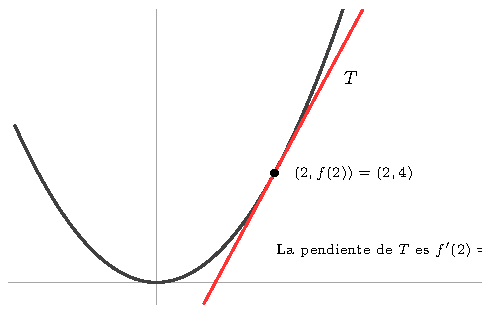
\includegraphics{figuras/recta-tangente.pdf}
        \caption{Gráfica de la función $f(x)=x^{2}$ y de su recta tangente $T$ en el punto $(2,4)$.}
        \label{fig:5.7}
    \end{figure}

    \begin{ejemplo}[Velocidad, rapidez y aceleración de un objeto]\label{ejm:85}
        La función
        de posición $s(t)$ de un objeto que se mueve en línea recta está dada
        por
        \begin{equation*}
            s(t)=40\sin\left(\frac{\pi}{2}t+\frac{\pi}{2}\right).
        \end{equation*}
        Si la distancia se mide en centímetros y el tiempo en segundos,
        \begin{enumerate}[nosep]
            \item ¿Cuál es la posición inicial $s(0)$ del objeto?
            \item ¿Cuál es la velocidad inicial $v(0)$ del objeto?
            \item ¿Cuál es la rapidez inicial $r(0)$ del objeto?
            \item ¿Cuál es la aceleración inicial $a(0)$ del objeto?
            \item ¿Cuál es la posición del objeto en el instante $t=3$?
            \item ¿Cuál es la velocidad del objeto en el instante $t=3$?
            \item ¿Cuál es la rapidez del objeto en el instante $t=3$?
            \item ¿Cuál es la aceleración del objeto en el instante $t=3$?
        \end{enumerate}

        \textbf{Solución.} La posición inicial del objeto es el punto $s(0)=40$ y la posición
        del objeto en el instante $t=3$ es el punto $s(3)=0$. Como
        \begin{equation*}
            v(t)=s'(t)=20\pi\cos\left(\frac{\pi}{2}t+\frac{\pi}{2}\right),
        \end{equation*}
        entonces la velocidad inicial del objeto es $v(0)=0$ cm/s, la velocidad del
        objeto en el instante $t=3$ es $v(3)=20\pi$ cm/s, la rapidez inicial del objeto
        es $r(0)=|v(0)|=0$ cm/s y la rapidez del objeto en el instante $t=3$ es
        $r(3)=|v(3)|=20\pi$ cm/s. Finalmente, puesto que
        \begin{equation*}
            a(t)=v'(t)=-10\pi^{2}\sin\left(\frac{\pi}{2}t+\frac{\pi}{2}\right),
        \end{equation*}
        entonces la aceleración inicial del objeto es $a(0)=-10\pi^{2}$ cm/s$^{2}$ y la aceleración
        del objeto en el instante $t=3$ es $a(3)=0$ cm/s$^{2}$.
    \end{ejemplo}

    El anterior es un ejemplo de un objeto que tiene un movimiento armónico
    simple, por ejemplo, un objeto atado al extremo de un resorte en movimiento.
    El lector interesado en el movimiento armónico simple puede consultar \cite{nunez2020mecanica}
    o cualquier libro de mecánica clásica.

    \begin{ejemplo}[Razón de cambio]\label{ejm:86}
        La temperatura $T(t)$ de la lava (recién
        expulsada) de cierto volcán en el instante $t$ está dada por
        \begin{equation*}
            T(t)=24+1176e^{-2t}.
        \end{equation*}
        Si la temperatura está dada en grados centígrados y el tiempo en horas, ¿cuál
        es la temperatura inicial $T(0)$ de la lava?, ¿cuál es la temperatura de la lava
        a las dos horas?, ¿cuál es la razón de cambio de la temperatura de la lava
        $T(t)$ respecto al tiempo en el instante $t=2$?

        \textbf{Solución.} La temperatura inicial de la lava es $T(0)=1200$ °C. La temperatura
        de la lava a las dos horas es $T(2)\approx 45.5391$ °C. Finalmente, como
        \begin{equation*}
            T'(t)=-2352e^{-2t},
        \end{equation*}
        entonces la razón de cambio de la temperatura de la lava $T(t)$ respecto al
        tiempo en el instante $t=2$ es $T'(2)\approx -43.0783$ °C/h.
    \end{ejemplo}

    \par\avoidorphan{6}\subsection*{Ejercicios}

    \begin{ejercicio}\label{ej:234}
        Calcula la derivada de las funciones siguientes (puedes usar
        todas las fórmulas de derivación que vimos en esta sección):
        \begin{multicols}{2}
        \begin{enumerate}[nosep]
            \item $3x^{5}-2x^{4}+8x+11$.
            \item $-x^{4}+x^{2}+5x-2$.
            \item $\left(4x^{7}+x\right)(\cos(x)-3x)$
            \item $\frac{-5x^{4}+3x^{3}-2x}{8x^{3}+9x}$.
            \item $\frac{\ln(x)x}{x^{2}+1}+9xe^{x}-5x$.
            \item $\sin\left(x^{4}+1\right)$.
            \item $\tan\left(x^{3}+x\right)$
            \item $\sin^{5}\left(x^{2}+3x\right)$.
            \item $\tan^{3}(7x+4)$.
            \item $\ln\left(6x^{4}+11x^{2}\right)$.
            \item $\ln(\sin(5x+9))$.
            \item $e^{7x^{3}+4x^{-3}}$.
            \item $e^{4x\sin(x)+2x^{5}}$.
            \item[(n)] $\sqrt{x^{2}-1}$.
            \item[(ñ)] $\sqrt[3]{2x^{3}-8x}$.
            \item[(o)] $\ln(1+\sin(2x))$.
            \item[(p)] $\sin\left(x^{4}+1\right)\sqrt{x^{2}-1}$.
            \item[(q)] $\sin\left(\sqrt{2x^{3}-x}\right)$.
            \item[(r)] $\sqrt{\sin\left(2x^{3}-x\right)}$.
            \item[(s)] $\sqrt{\sqrt{x^{2}}}+\sin(x-\cos(x))$.
        \end{enumerate}
        \end{multicols}
    \end{ejercicio}

    \begin{ejercicio}\label{ej:235}
        Calcula la derivada de la función valor absoluto $|x|$.
    \end{ejercicio}

    \begin{ejercicio}\label{ej:236}
        Calcula la derivada de la función
        \begin{equation*}
            f(x)=\begin{cases}
                1, & \text{si }x\geq 0,\\
                -1, & \text{si }x<0.
            \end{cases}
        \end{equation*}
    \end{ejercicio}

    \begin{ejercicio}\label{ej:237}
        Calcula la derivada de la función
        \begin{equation*}
            f(x)=\begin{cases}
                x^{2}, & \text{si }x\neq 2,\\
                5, & \text{si }x=2.
            \end{cases}
        \end{equation*}
    \end{ejercicio}

    \begin{ejercicio}\label{ej:238}
        Calcula la derivada de la función
        \begin{equation*}
            f(x)=\begin{cases}
                x^{3}, & \text{si }x<-1,\\
                x, & \text{si }-1\leq x<1,\\
                x^{2}+2x, & \text{si }1\leq x.
            \end{cases}
        \end{equation*}
    \end{ejercicio}

    \begin{ejercicio}\label{ej:239}
        Sea $n$ un número natural. Prueba que
        \begin{equation*}
            \frac{d}{dx}(x^{n})=nx^{n-1}.
        \end{equation*}
        \sugerencia Usa el principio de inducción matemática y la fórmula de la
        derivada de un producto.
    \end{ejercicio}

    \begin{ejercicio}\label{ej:240}
        Sea $n$ un número natural con $n\geq 2$. Prueba que
        \begin{equation*}
            \frac{d}{dx}\left(x^{\frac{1}{n}}\right)=\frac{1}{n}x^{\frac{1}{n}-1},\ \ x\neq 0.
        \end{equation*}
        \sugerencia Usa la fórmula de la derivada de la función inversa.
    \end{ejercicio}

    \begin{ejercicio}\label{ej:241}
        Sea $r$ un número racional. Prueba que
        \begin{equation*}
            \frac{d}{dx}(x^{r})=rx^{r-1},\ \ x>0.
        \end{equation*}
        En \cite{nunez2020calculoII} mostraremos que la fórmula anterior también se cumple para cualquier
        número real $r$. \sugerencia Ten en cuenta los ejercicios~\ref{ej:239} y~\ref{ej:240}.
    \end{ejercicio}

    \begin{ejercicio}\label{ej:242}
        Si $f(x)=(x-5)^{3}+\sqrt{x-2}$, calcula $\left(f^{-1}\right)'(3)$. Ten en cuenta
        que $f(6)=3$.
    \end{ejercicio}

    \begin{ejercicio}\label{ej:243}
        Si $g(x)=7(x-1)^{3}e^{x-2}$, calcula $\left(g^{-1}\right)'(7)$. Ten en cuenta
        que $g(2)=7$.
    \end{ejercicio}

    \begin{ejercicio}\label{ej:244}
        Si $h(x)=\ln(x+1)+x\sqrt{x+1}$, calcula $\left(h^{-1}\right)'(0)$. Ten en
        cuenta que $h(0)=0$.
    \end{ejercicio}

    \begin{ejercicio}[Derivada de la función exponencial]\label{ej:245}
        Como comentamos
        anteriormente, la función exponencial $e^{x}$ es la función inversa de la función
        logaritmo natural $\ln(x)$. Sabiendo que para $x>0$,
        \begin{equation*}
            \ln'(x)=\frac{1}{x},
        \end{equation*}
        prueba que la derivada de la función exponencial $e^{x}$ es la función exponencial
        $e^{x}$.
    \end{ejercicio}

    \begin{ejercicio}\label{ej:246}
        Prueba que
        \begin{equation*}
            \frac{d}{dx}\ln(|x|)=\frac{1}{x},\ \ x\neq 0.
        \end{equation*}
        \sugerencia Considera los casos en que $x>0$ y $x<0$.
    \end{ejercicio}

    \begin{ejercicio}\label{ej:247}
        Sea $f(x)=5-x^{2}$.
        \begin{enumerate}[nosep]
            \item Dibuja la gráfica de $f$.
            \item Encuentra la pendiente de la recta tangente $T$ a la gráfica de $f$ en el punto
            $(2,1)$.
            \item Encuentra la ecuación de $T$.
            \item Dibuja la gráfica de $T$.
        \end{enumerate}
    \end{ejercicio}

    \begin{ejercicio}\label{ej:248}
        Sea $f(x)=x^{3}+1$.
        \begin{enumerate}[nosep]
            \item Dibuja la gráfica de $f$.
            \item Encuentra la pendiente de la recta tangente $T$ a la gráfica de $f$ en el punto
            $(1,2)$.
            \item Encuentra la ecuación de $T$.
            \item Dibuja la gráfica de $T$.
        \end{enumerate}
    \end{ejercicio}

    \begin{ejercicio}\label{ej:249}
        Encuentra la ecuación de la recta tangente a la gráfica de la
        función $f(x)=x^{3}+2$ en el punto $(1,f(1))=(1,3)$.
    \end{ejercicio}

    \begin{ejercicio}\label{ej:250}
        Encuentra la ecuación de la recta tangente a la gráfica de la
        función $f(x)=e^{x-2}$ en el punto $(2,f(2))=(2,1)$.
    \end{ejercicio}

    \begin{ejercicio}\label{ej:251}
        Encuentra la ecuación de la recta tangente a la gráfica de la
        función $f(x)=\ln(x)+x$ en el punto $(1,f(1))=(1,1)$.
    \end{ejercicio}

    \begin{ejercicio}\label{ej:252}
        La recta tangente a la gráfica de una función $f$ en el punto
        $(1,2)$ pasa por el punto $(3,4)$. Encuentra $f(1)$ y $f'(1)$.
    \end{ejercicio}

    \begin{ejercicio}\label{ej:253}
        La recta tangente a la gráfica de una función $f$ en el punto
        $(0,3)$ pasa por el punto $(1,5)$. Encuentra $f(0)$ y $f'(0)$.
    \end{ejercicio}

    \begin{ejercicio}[Caída libre]\label{ej:254}
        \index{caida libre@caída libre}Se deja caer una piedra desde un edificio de
        $100$ m de altura. La altura de la piedra en el instante $t$ (antes de tocar el
        suelo) está dada por la función
        \begin{equation*}
            h(t)=-\frac{98}{20}t^{2}+100,\ \ t\geq 0.
        \end{equation*}
        Si la distancia se mide en metros y el tiempo en segundos, responde lo
        siguiente:
        \begin{enumerate}[nosep]
            \item ¿Cuánto tiempo tarda en caer la piedra (hasta el suelo)? Ten en cuenta
            que el instante $t$ en que la piedra toca el suelo es cuando $h(t)=0$.
            \item ¿Cuál es la velocidad inicial de la piedra?
            \item ¿Cuál es la rapidez inicial de la piedra?
            \item ¿Cuál es la aceleración inicial de la piedra?
            \item ¿Cuál es la velocidad de la piedra al tocar el suelo?
            \item ¿Cuál es la rapidez de la piedra al tocar el suelo?
            \item ¿Cuál es la aceleración de la piedra al tocar el suelo?
        \end{enumerate}
        Este es un ejemplo de un objeto en \textit{caída libre} (objeto que describe un movimiento
        rectilíneo con aceleración constante debida a la gravedad).
    \end{ejercicio}

    \begin{ejercicio}[Caída libre]\label{ej:255}
        \index{caida libre@caída libre}La función de posición (altura) $s(t)$ de un
        proyectil que se lanza desde el suelo y hacia arriba (verticalmente) está dada
        por la función
        \begin{equation*}
            s(t)=-\frac{98}{20}t^{2}+340t,\ \ t\geq 0.
        \end{equation*}
        Si la distancia se mide en metros y el tiempo en segundos, responde lo
        siguiente:
        \begin{enumerate}[nosep]
            \item ¿Cuál es la velocidad inicial del proyectil?
            \item ¿Cuál es la rapidez inicial del proyectil?
            \item ¿Cuál es la aceleración inicial del proyectil?
            \item ¿Cuál es la altura máxima del proyectil? Ten en cuenta que el instante en
            que el proyectil alcanza su altura máxima es cuando $v(t)=0$.
            \item ¿En qué instante $t$ el proyectil vuelve a tocar el suelo? Ten en cuenta que
            si el proyectil toca el suelo en un instante $t$, entonces $s(t)=0$.
            \item ¿Cuál es la velocidad del proyectil al tocar el suelo?
            \item ¿Cuál es la rapidez del proyectil al tocar el suelo?
            \item ¿Cuál es la aceleración del proyectil al tocar el suelo?
        \end{enumerate}
        Este es otro ejemplo de un objeto en \textit{caída libre} (objeto que describe un
        movimiento rectilíneo con aceleración constante debida a la gravedad).
    \end{ejercicio}

    En \cite{nunez2020calculoII} mostraremos que la función de posición $s(t)$ de un objeto que se
    mueve en línea recta con aceleración constante $\alpha$ (a este tipo de movimiento
    se le llama \textit{movimiento rectilíneo uniformemente acelerado}\index{movimiento rectilineo uniformemente acelerado@movimiento rectilíneo uniformemente acelerado} (MRUA)) tiene
    la forma
    \begin{equation*}
        s(t)=\frac{1}{2}\alpha t^{2}+v_{0}t+s_{0},
    \end{equation*}
    donde $s_{0}$ es la posición inicial del objeto y $v_{0}$ es la velocidad inicial del objeto.
    Los dos ejercicios anteriores son ejemplos de MRUA con aceleración constante
    $-g=-9.8$ m/s$^{2}$ debida a la gravedad de la tierra a nivel del mar.

    \begin{ejercicio}[Derivada de las funciones trigonométricas inversas]\label{ej:256}
        \index{derivada de las funciones trigonometricas inversas@derivada de las funciones trigonométricas inversas}Usa la proposición~\ref{prop:62} (derivada de una función inversa) para mostrar lo
        siguiente:
        \begin{enumerate}[nosep]
            \item $\arcsin'(x)=\frac{1}{\sqrt{1-x^{2}}}$, $-1<x<1$.
            \item $\arccos'(x)=\frac{-1}{\sqrt{1-x^{2}}}$, $-1<x<1$.
            \item $\arctan'(x)=\frac{1}{1+x^{2}}$, $-\infty<x<\infty$.
            \item $\arccot'(x)=\frac{-1}{1+x^{2}}$, $-\infty<x<\infty$.
            \item $\arcsec'(x)=\begin{cases}\frac{1}{x\sqrt{x^{2}-1}}, & x>1,\\ \frac{-1}{x\sqrt{x^{2}-1}}, & x<-1.\end{cases}$
            \item $\arccsc'(x)=\begin{cases}\frac{-1}{x\sqrt{x^{2}-1}}, & x>1,\\ \frac{1}{x\sqrt{x^{2}-1}}, & x<-1.\end{cases}$
        \end{enumerate}
        \sugerencia Por la proposición~\ref{prop:62} (derivada de una función inversa) sabemos
        que si $f(x)=\sin(x)$, entonces
        \begin{equation*}
            \arcsin'(x)=\frac{1}{f'\left(f^{-1}(x)\right)}=\frac{1}{\cos\left(f^{-1}(x)\right)},\ \ -1<x<1.
        \end{equation*}
        Puesto que $\sin^{2}(x)+\cos^{2}(x)=1$ para todo número real $x$, resulta que
        \begin{equation*}
            \sin^{2}\left(f^{-1}(x)\right)+\cos^{2}\left(f^{-1}(x)\right)=1,\ \ -1<x<1
        \end{equation*}
        y, en consecuencia, que
        \begin{equation*}
            \frac{1}{\cos\left(f^{-1}(x)\right)}=\frac{1}{\sqrt{1-x^{2}}},\ \ -1<x<1,
        \end{equation*}
        lo cual prueba el inciso (a). La prueba del inciso (b) es similar a la prueba
        del inciso (a). Para probar el inciso (c) usa que $\tan^{2}(x)+1=\sec^{2}(x)$; para
        probar el inciso (d) usa que $1+\cot^{2}(x)=\csc^{2}(x)$; para probar el inciso (e)
        usa que\footnote{Verificaremos esta igualdad en \cite{nunez2020calculoII}.}
        \begin{equation*}
            \tan(\arcsec(x))=\begin{cases}
                \sqrt{x^{2}-1}, & \text{si }x\geq 1,\\
                -\sqrt{x^{2}-1}, & \text{si }x\leq -1.
            \end{cases}
        \end{equation*}
        Finalmente, para probar el inciso (f) usa que\footnote{Verificaremos esta igualdad en \cite{nunez2020calculoII}.}
        \begin{equation*}
            \cot(\arccsc(x))=\begin{cases}
                \sqrt{x^{2}-1}, & \text{si }x\geq 1,\\
                -\sqrt{x^{2}-1}, & \text{si }x\leq -1.
            \end{cases}
        \end{equation*}
    \end{ejercicio}

    \begin{ejercicio}\label{ej:257}
        Realiza lo siguiente:
        \begin{enumerate}[nosep]
            \item Prueba que la función $\arcsin(x)$ no es derivable en $1$ y en $-1$.
            \item Prueba que la función $\arccos(x)$ no es derivable en $1$ y en $-1$.
            \item Prueba que la función $\arcsec(x)$ no es derivable en $1$ y en $-1$.
            \item Prueba que la función $\arccsc(x)$ no es derivable en $1$ y en $-1$.
        \end{enumerate}
    \end{ejercicio}

    \begin{ejercicio}\label{ej:258}
        Considera la función
        \begin{equation*}
            f(x)=\begin{cases}
                x\sin(1/x), & \text{si }x\neq 0,\\
                0, & \text{si }x=0.
            \end{cases}
        \end{equation*}
        La gráfica de $f$ aparece en la figura~\ref{fig:3.14}. Muestra que
        \begin{equation*}
            f'(x)=\begin{cases}
                \sin(1/x)-\cos(1/x)/x, & \text{si }x\neq 0,\\
                \text{no existe}, & \text{si }x=0.
            \end{cases}
        \end{equation*}
        \sugerencia Para probar que $f$ no es derivable en $0$ usa la definición de
        derivada y ten presente que $\lim_{x\to 0}\sin(1/x)$ no existe (véase el ejercicio~\ref{ej:158}).
    \end{ejercicio}

    \begin{ejercicio}[Una función con derivada no continua]\label{ej:259}
        Considera la
        función
        \begin{equation*}
            f(x)=\begin{cases}
                x^{2}\sin(1/x), & \text{si }x\neq 0,\\
                0, & \text{si }x=0.
            \end{cases}
        \end{equation*}
        La gráfica de $f$ aparece en la figura~\ref{fig:3.15}.
        \begin{enumerate}
            \item Muestra que
            \begin{equation*}
                f'(x)=\begin{cases}
                    2x\sin(1/x)-\cos(1/x), & \text{si }x\neq 0,\\
                    0, & \text{si }x=0.
                \end{cases}
            \end{equation*}
            \item Prueba que $f'$ no es continua en $0$.
        \end{enumerate}
        \sugerencia Para probar que $f$ es derivable en $0$ en el inciso (a) usa la
        definición de derivada y ten presente que $|\sin(x)|\leq 1$ para toda $x$. Para el
        inciso (b) procede por contradicción y ten presente que $\lim_{x\to 0}\cos(1/x)$ no
        existe (véase el ejercicio~\ref{ej:158}).
    \end{ejercicio}

    \section{Derivación Implícita}

    Hasta ahora hemos trabajado con funciones cuya regla de correspondencia
    ha sido dada de manera explícita, por ejemplo, $f(x)=x^{2}+1$ o $y=x^{2}+1$.
    En este caso, en la ecuación $y=x^{2}+1$, la función $y$ aparece despejada. Sin
    embargo, podemos definir una función $y$ de manera implícita mediante una
    ecuación, por ejemplo, la ecuación
    \begin{equation}\label{eq:5.18}
        y^{3}+3y-2x=0
    \end{equation}
    define una función $y$, pues a cada $x$ la ecuación \eqref{eq:5.18} le asigna un único valor
    $y$ (véanse la figura~\ref{fig:5.8} y el ejercicio~\ref{ej:266}). En este caso, en la ecuación \eqref{eq:5.18}
    la función $y$ no aparece despejada, esta es la razón por la cual se dice que la
    función $y$ está dada de manera implícita. El cuadro siguiente muestra algunos
    valores de la función $y$ definida implícitamente por la ecuación \eqref{eq:5.18}.
    \begin{center}
        \renewcommand{\arraystretch}{1.3}
        \begin{tabular}{|p{3.5cm}|p{3.5cm}|}
            \hline
            \multicolumn{2}{|c|}{\celda{\textbf{Algunos valores de la función $\boldsymbol{y}$}\\ \textbf{definida por la ecuación \eqref{eq:5.18}.}}}\\ \hline\noalign{\vskip 3pt}\hline
            \multicolumn{1}{|c|}{$x$} & \multicolumn{1}{c|}{$y$}\\ \hline
            \multicolumn{1}{|c|}{$0$} & \multicolumn{1}{c|}{$0$}\\ \hline
            \multicolumn{1}{|c|}{$2$} & \multicolumn{1}{c|}{$1$}\\ \hline
            \multicolumn{1}{|c|}{$7$} & \multicolumn{1}{c|}{$2$}\\ \hline
        \end{tabular}
    \end{center}

    \begin{figure}[H]
        \centering
        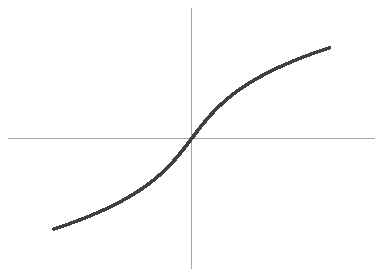
\includegraphics{figuras/implicita-cubica.pdf}
        \caption{Gráfica de la ecuación $y^{3}+3y-2x=0$.}
        \label{fig:5.8}
    \end{figure}

    No toda ecuación en las variables $x$ y $y$ define una función $y$, por ejemplo,
    la ecuación
    \begin{equation}\label{eq:5.19}
        x^{2}+y^{2}-1=0
    \end{equation}
    no define una función $y$, pues la ecuación \eqref{eq:5.19} asigna al número $0$ dos valores
    para $y$, el $1$ y el $-1$ (véase la figura~\ref{fig:5.9}). Para obtener una función $y$ a partir
    de la ecuación \eqref{eq:5.19} podemos, por ejemplo, considerar las partes superior
    $G_{1}$ e inferior $G_{2}$ de la gráfica de la ecuación \eqref{eq:5.19} (véase la figura~\ref{fig:5.10}). Así,
    la parte $G_{1}$ genera a la función
    \begin{equation*}
        y_{1}=\sqrt{1-x^{2}}
    \end{equation*}
    y la parte $G_{2}$ a la función
    \begin{equation*}
        y_{2}=-\sqrt{1-x^{2}}.
    \end{equation*}

    De aquí en adelante, si decimos que $y$ es una función definida implícitamente
    por una ecuación en las variables $x$ y $y$, supondremos que hemos
    cortado a la gráfica de tal ecuación en partes y que alguna de esas partes
    genera a la función $y$.

    \begin{figure}[H]
        \centering
        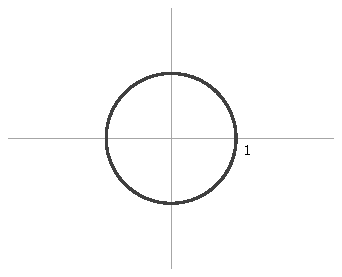
\includegraphics{figuras/circunferencia.pdf}
        \caption{Gráfica de la ecuación $x^{2}+y^{2}-1=0$.}
        \label{fig:5.9}
    \end{figure}

    \begin{figure}[H]
        \centering
        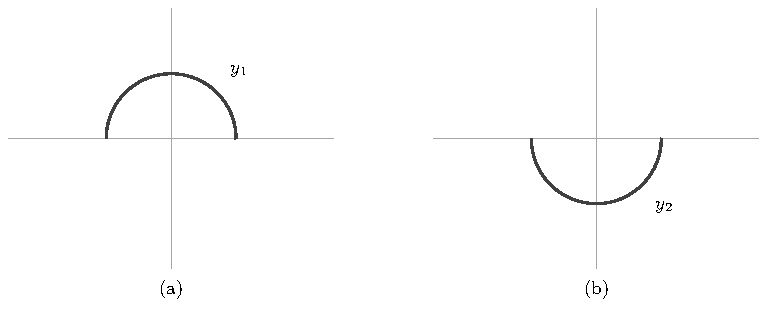
\includegraphics{figuras/semicircunferencias.pdf}
        \caption{Podemos partir la gráfica de la ecuación $x^{2}+y^{2}-1=0$ para obtener dos
        funciones $y_{1}$ y $y_{2}$.}
        \label{fig:5.10}
    \end{figure}

    \begin{definicion}[Derivación implícita]\label{def:49}
        Al proceso de encontrar la derivada
        de una función definida de manera implícita se le llama \textit{derivación implícita}\index{derivacion implicita@derivación implícita}.
    \end{definicion}

    Ahora veamos como se deriva una función definida de manera implícita.
    La mejor manera de mostrar esto es con un ejemplo.

    \begin{ejemplo}[Derivación implícita]\label{ejm:87}
        Encuentra la derivada de la función
        $y$ definida implícitamente por la ecuación
        \begin{equation}\label{eq:5.20}
            y^{3}+3xy-2x=0.
        \end{equation}

        \textbf{Solución.} Notemos primero que como $y$ es una función de $x$, entonces por
        la regla de la cadena,
        \begin{equation*}
            \left(y^{3}\right)'=3y^{2}\cdot y',
        \end{equation*}
        y por la fórmula de la derivada de un producto,
        \begin{align*}
            (3xy)'&=3(xy)'\\
            &=3(x'y+xy')\\
            &=3(y+xy')\\
            &=3y+3xy'.
        \end{align*}
        En consecuencia, al derivar ambos lados de la ecuación \eqref{eq:5.20} obtenemos que
        \begin{align*}
            0&=\left(y^{3}+3xy-2x\right)'\\
            &=\left(y^{3}\right)'+(3xy)'-(2x)'\\
            &=3y^{2}\cdot y'+3y+3xy'-2\\
            &=y'\left(3y^{2}+3x\right)+3y-2 &&\text{(factorizando $y'$)}.
        \end{align*}
        Luego, al despejar $y'$ obtenemos que
        \begin{equation*}
            y'=\frac{2-3y}{3y^{2}+3x}.\finej
        \end{equation*}
    \end{ejemplo}

    \begin{ejemplo}\label{ejm:88}
        Encuentra, usando derivación implícita, la ecuación de la recta
        tangente $T$ a la gráfica de la elipse
        \begin{equation}\label{eq:5.21}
            \frac{(x-3)^{2}}{4}+\left(y-\left(1+\sqrt{3}/2\right)\right)^{2}=1
        \end{equation}
        en el punto $(4,1)$ (véase la figura~\ref{fig:5.11}).

        \textbf{Solución.} Podemos escribir la ecuación \eqref{eq:5.21} como
        \begin{equation}\label{eq:5.22}
            (x-3)^{2}+4\left(y-1-\sqrt{3}/2\right)^{2}=4.
        \end{equation}
        Al derivar implícitamente a $y$ en la ecuación \eqref{eq:5.22} obtenemos que
        \begin{align*}
            0&=\left[(x-3)^{2}+4\left(y-1-\sqrt{3}/2\right)^{2}\right]'\\
            &=\left[(x-3)^{2}\right]'+4\left[\left(y-1-\sqrt{3}/2\right)^{2}\right]'\\
            &=2(x-3)+4\cdot 2\left(y-1-\sqrt{3}/2\right)\cdot y'.
        \end{align*}
        Luego,
        \begin{align*}
            y'&=\frac{2(3-x)}{8\left(y-1-\sqrt{3}/2\right)}\\
            &=\frac{3-x}{4\left(y-1-\sqrt{3}/2\right)}\\
            &=\frac{3-x}{4y-4-2\sqrt{3}}.
        \end{align*}
        Para nuestros propósitos, supondremos que $y$ es la función generada por la
        mitad inferior de la elipse, así que si $x=4$, entonces $y=1$ y, en consecuencia,
        $y'$ evaluada en $4$ es
        \begin{equation*}
            y'=\frac{3-4}{4-4-2\sqrt{3}}=\frac{1}{2\sqrt{3}}.
        \end{equation*}
        Como $y'$ evaluada en $4$ es la pendiente de $T$ y $T$ pasa por el punto $(4,1)$,
        entonces (según la ecuación de la forma punto pendiente de la recta) la ecuación
        de $T$ es
        \begin{equation*}
            \frac{y-1}{x-4}=\frac{1}{2\sqrt{3}}.
        \end{equation*}
        Simplificando obtenemos que la ecuación de $T$ es
        \begin{equation*}
            y=\frac{x}{2\sqrt{3}}+1-\frac{2}{\sqrt{3}}.\finej
        \end{equation*}
    \end{ejemplo}

    \begin{figure}[H]
        \centering
        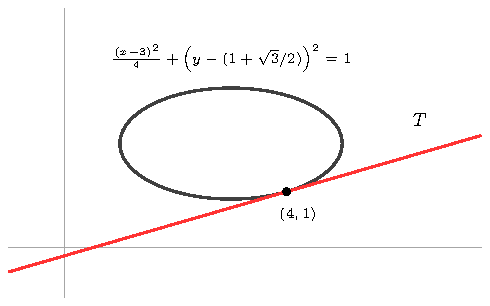
\includegraphics{figuras/elipse-tangente.pdf}
        \caption{Elipse $(x-3)^{2}/4+\left(y-\left(1+\sqrt{3}/2\right)\right)^{2}=1$ y su recta tangente $T$ en $(4,1)$.}
        \label{fig:5.11}
    \end{figure}

    \par\avoidorphan{6}\subsection*{Ejercicios}

    \begin{ejercicio}\label{ej:260}
        Deriva implícitamente a las funciones $y$ definidas implícitamente
        por las ecuaciones siguientes:
        \begin{multicols}{2}
        \begin{enumerate}[nosep]
            \item $10xy^{2}+y=1$.
            \item $y^{3}x+3xy^{3}-1=0$.
            \item $7x\sin(y)+y=10$.
            \item $\sin(xy)+xy=7$.
        \end{enumerate}
        \end{multicols}
    \end{ejercicio}

    \begin{ejercicio}\label{ej:261}
        Realiza lo siguiente:
        \begin{enumerate}[nosep]
            \item Dibuja la elipse
            \begin{equation*}
                \frac{x^{2}}{2}+\frac{y^{2}}{4}=1.
            \end{equation*}
            \item Usa derivación implícita para calcular la pendiente de la recta tangente $T$
            a la elipse del inciso (a) en el punto $(1,\sqrt{2})$.
            \item Encuentra la ecuación de $T$.
            \item Dibuja la gráfica de $T$.
        \end{enumerate}
    \end{ejercicio}

    \begin{ejercicio}\label{ej:262}
        Realiza lo siguiente:
        \begin{enumerate}[nosep]
            \item Dibuja la hipérbola
            \begin{equation*}
                \frac{x^{2}}{4}-\frac{y^{2}}{2}=1.
            \end{equation*}
            \item Usa derivación implícita para calcular la pendiente de la recta tangente $T$
            a la hipérbola del inciso (a) en el punto $(3,\sqrt{5/2})$.
            \item Encuentra la ecuación de $T$.
            \item Dibuja la gráfica de $T$.
        \end{enumerate}
    \end{ejercicio}

    \begin{ejercicio}\label{ej:263}
        Realiza lo siguiente:
        \begin{enumerate}[nosep]
            \item Dibuja la circunferencia
            \begin{equation*}
                x^{2}+y^{2}=4y.
            \end{equation*}
            \item Usa derivación implícita para calcular la pendiente de la recta tangente $T$
            a la circunferencia del inciso (a) en el punto $(1,2+\sqrt{3})$.
            \item Encuentra la ecuación de $T$.
            \item Dibuja la gráfica de $T$.
        \end{enumerate}
    \end{ejercicio}

    \begin{ejercicio}\label{ej:264}
        Encuentra la ecuación de la recta tangente $T$ a la gráfica de
        la lemniscata
        \begin{equation*}
            \left(x^{2}+y^{2}\right)^{2}=2\left(x^{2}-y^{2}\right)
        \end{equation*}
        en el punto $\left(\sqrt{3}/2,1/2\right)$.
    \end{ejercicio}

    \begin{ejercicio}\label{ej:265}
        Encuentra la ecuación de la recta tangente $T$ a la gráfica del
        cardioide
        \begin{equation*}
            \left(x^{2}+y^{2}-2x\right)^{2}=4\left(x^{2}+y^{2}\right)
        \end{equation*}
        en el punto $(0,2)$.
    \end{ejercicio}

    \begin{ejercicio}\label{ej:266}
        Muestra que para cada número real $x$ existe un único $y$ que
        satisface la ecuación
        \begin{equation}\label{eq:5.23}
            y^{3}+3y-2x=0.
        \end{equation}
        \sugerencia Para probar que dado $x$, existe un $y$ que cumple \eqref{eq:5.23} usa
        que el rango de la función $f(t)=t^{3}+3t$ es todo $\R$ (véase el ejercicio~\ref{ej:210}).
        Para probar la unicidad de tal $y$ supón lo contrario, es decir, supón que
        existen dos valores distintos $y_{1}$ y $y_{2}$ que cumplen \eqref{eq:5.23}; usa que la función
        $g(t)=t^{3}+3t-2x$ es 1-1 para obtener una contradicción.
    \end{ejercicio}

    \section{Mínimos y Máximos Locales}

    En esta sección introduciremos y estudiaremos los conceptos de mínimo
    local y máximo local de una función, conceptos cruciales en las aplicaciones,
    como lo veremos en las próximas secciones.

    \begin{definicion}[Mínimos y máximos locales]\label{def:50}
        Sea $f$ una función.
        \begin{enumerate}
            \item Diremos que $f(p)$ es un \textit{mínimo local}\index{minimo local de una funcion@mínimo local de una función} de $f$ si existe un intervalo abierto $I$
            que contiene a $p$ tal que
            \begin{equation*}
                f(p)\leq f(x)\ \text{ para todo }x\in I.
            \end{equation*}
            En este caso se dice que $f$ alcanza un mínimo local en $p$.
            \item Diremos que $f(p)$ es un \textit{máximo local}\index{maximo local de una funcion@máximo local de una función} de $f$ si existe un intervalo abierto $I$
            que contiene a $p$ tal que
            \begin{equation*}
                f(x)\leq f(p)\ \text{ para todo }x\in I.
            \end{equation*}
            En este caso se dice que $f$ alcanza un máximo local en $p$.
        \end{enumerate}
    \end{definicion}

    A los mínimos y máximos locales de una función también se les llama
    \textit{extremos locales}\index{extremos locales de una funcion@extremos locales de una función} de la función. La figura~\ref{fig:5.12} muestra algunos mínimos y
    máximos locales de una función y los puntos donde se alcanzan.

    La proposición siguiente será de gran ayuda para encontrar los máximos
    y mínimos locales de una función.

    \begin{proposicion}\label{prop:63}
        Sea $f$ una función definida en un intervalo abierto $I$. Si $f$
        alcanza un mínimo local o máximo local en $p$, entonces $f'(p)=0$ o $f'(p)$ no
        existe (véase la figura~\ref{fig:5.13}).
    \end{proposicion}

    \begin{figure}[H]
        \centering
        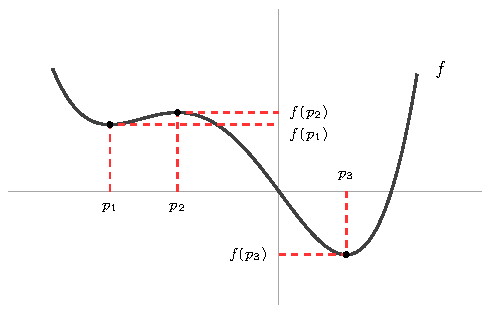
\includegraphics{figuras/extremos-locales.pdf}
        \caption{Los números $f(p_{1})$ y $f(p_{3})$ son mínimos locales de $f$ y el número $f(p_{2})$ es
        un máximo local de $f$.}
        \label{fig:5.12}
    \end{figure}

    \begin{proof}
        Supongamos que $f$ alcanza un mínimo local en $p$, la prueba
        en el caso en que $f$ alcanza un máximo local en $p$ es similar. Sabemos que
        $f'(p)$ existe o $f'(p)$ no existe. Así, basta probar que si $f'(p)$ existe, entonces
        $f'(p)=0$. Supongamos pues que $f$ es derivable en $p$. Puesto que $f$ alcanza
        un mínimo local en $p$, entonces existe un intervalo abierto $J$ que contiene a
        $0$ tal que
        \begin{equation*}
            f(p+h)-f(p)\geq 0,\ \ h\in J.
        \end{equation*}
        Así,
        \begin{equation*}
            \lim_{h\to 0^{-}}\frac{f(p+h)-f(p)}{h}\leq 0
        \end{equation*}
        y
        \begin{equation*}
            \lim_{h\to 0^{+}}\frac{f(p+h)-f(p)}{h}\geq 0.
        \end{equation*}
        Por lo tanto, por el criterio de los límites laterales obtenemos que
        \begin{equation*}
            f'(p)=\lim_{h\to 0}\frac{f(p+h)-f(p)}{h}=0.\qedhere
        \end{equation*}
    \end{proof}

    El recíproco de la proposición anterior no es cierto, por ejemplo, si $f(x)=
    x^{3}$, entonces $f'(0)=0$ y, sin embargo, $f(0)$ no es ni mínimo local ni máximo
    local de $f$. Por otra parte, si definimos
    \begin{equation*}
        g(x)=\begin{cases}
            -1, & \text{si }x<0,\\
            0, & \text{si }x=0,\\
            1, & \text{si }x>0,
        \end{cases}
    \end{equation*}
    entonces $g'(0)$ no existe, y sin embargo, $g(0)$ no es ni mínimo local ni máximo
    local de $g$.

    \begin{figure}[H]
        \centering
        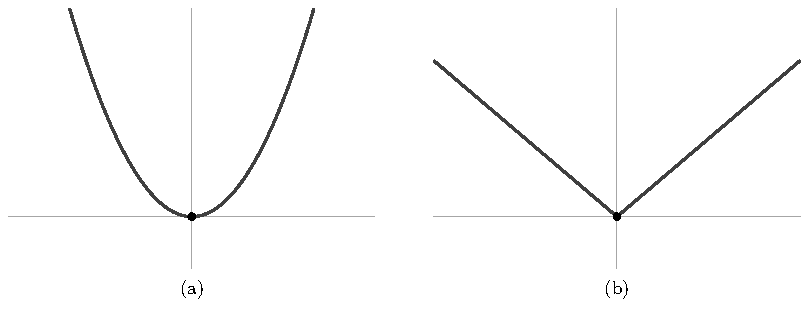
\includegraphics{figuras/extremo-derivada.pdf}
        \caption{(a) La función $f(x)=x^{2}$ alcanza un mínimo local en $0$ y $f'(0)=0$. (b) La
        función $f(x)=|x|$ alcanza un mínimo local en $0$ y $f'(0)$ no existe.}
        \label{fig:5.13}
    \end{figure}

    Entre otras cosas, por la proposición anterior, los puntos $p$ tales que
    $f'(p)=0$ o que $f'(p)$ no existe merecen un nombre especial.

    \begin{definicion}[Punto crítico]\label{def:51}
        Sea $f$ una función. Diremos que $p$ es un
        \textit{punto crítico}\index{punto critico de una funcion@punto crítico de una función} de $f$ si
        \begin{equation*}
            f'(p)=0\text{ o si }f'(p)\text{ no existe.}
        \end{equation*}
    \end{definicion}

    Más adelante, en la subsección~\ref{subsec:criterios}, veremos como calcular los mínimos
    y máximos locales de una función.

    Para finalizar esta pequeña sección, como consecuencia del teorema del mínimo
    y máximo (teorema~\ref{teo:2}) y de la proposición~\ref{prop:63}, mostraremos que, al igual
    que las funciones continuas, la derivada de una función (cuya derivada existe
    en todo un intervalo con más de un punto) alcanza sus valores intermedios.

    \begin{teorema}[del valor intermedio para derivadas]\label{teo:6}
        \index{teorema del valor intermedio para derivadas}Si $f:[a,b]\to\R$ es
        derivable\footnote{Recordemos que una función $f$ es derivable en un intervalo cerrado $[a,b]$ con $a<b$ si $f$
        es derivable en el intervalo abierto $(a,b)$ y si $f'(a)$ y $f'(b)$ existen como límites laterales.} y $c$ es un número con
        \begin{equation*}
            f'(a)<c<f'(b)\ \text{ o }\ f'(b)<c<f'(a),
        \end{equation*}
        entonces existe $x\in(a,b)$ tal que $f'(x)=c$.
    \end{teorema}

    \begin{proof}
        Supongamos que $f'(a)<c<f'(b)$, el caso en que $f'(b)<
        c<f'(a)$ se prueba de manera similar. Definamos $g(x)=f(x)-cx$. Por
        el teorema del mínimo y máximo (teorema~\ref{teo:2}) sabemos que $g$ tiene mínimo.
        Probaremos que el mínimo de $g$ se alcanza en algún punto $x$ del intervalo
        $(a,b)$ y, en consecuencia, por la proposición~\ref{prop:63}, tendremos que $g'(x)=0$,
        de lo cual obtendremos lo afirmado. Como $g'(a)=f'(a)-c<0$, entonces
        existe $\delta_{1}>0$ tal que si $h\in(0,\delta_{1})$, entonces
        \begin{equation*}
            \frac{g(a+h)-g(a)}{h}<0,
        \end{equation*}
        de lo cual resulta que si $h\in(0,\delta_{1})$, entonces $g(a+h)<g(a)$. De manera
        similar, existe $\delta_{2}>0$ tal que si $h\in(-\delta_{2},0)$, entonces $g(b+h)<g(b)$. En
        consecuencia, $g$ alcanza su mínimo en algún punto $x$ del intervalo $(a,b)$.
    \end{proof}

    Notemos que a diferencia del teorema del valor intermedio (teorema~\ref{teo:3})
    en el teorema del valor intermedio para derivadas (teorema~\ref{teo:6}) no se pide la
    continuidad de $f'$ en el intervalo cerrado $[a,b]$, se pide simplemente que $f'$
    exista en todo $[a,b]$.

    \section{El Teorema del Valor Medio}

    En esta sección, como consecuencia del teorema del mínimo y máximo
    (teorema~\ref{teo:2}) y de la proposición~\ref{prop:63}, probaremos el teorema del valor medio
    generalizado del cual obtendremos el teorema del valor medio, uno de los
    teoremas más importantes sobre la derivada. La utilidad del teorema del
    valor medio y del teorema del valor medio generalizado se apreciará en las
    próximas secciones.

    Enunciamos primero el teorema del valor medio.

    \begin{teorema}[del valor medio]\label{teo:7}
        \index{teorema del valor medio}Sea $f$ una función continua en un intervalo
        $[a,b]$ y derivable en el intervalo $(a,b)$. Entonces existe $c\in(a,b)$ tal que
        \begin{equation*}
            f(b)-f(a)=f'(c)(b-a).
        \end{equation*}
    \end{teorema}

    El significado geométrico del teorema del valor medio (véase la figura~\ref{fig:5.14})
    es que existe $c\in(a,b)$ tal que la recta tangente a la gráfica de $f$ en el punto
    $(c,f(c))$ y el segmento de recta que une los puntos $(a,f(a))$ y $(b,f(b))$ tienen
    la misma pendiente.

    Ahora enunciamos y probamos el teorema del valor medio generalizado.

    \begin{teorema}[del valor medio generalizado]\label{teo:8}
        \index{teorema del valor medio generalizado}Sean $f$ y $g$ funciones continuas
        en un intervalo $[a,b]$ y derivables en el intervalo $(a,b)$. Entonces existe
        $c\in(a,b)$ tal que
        \begin{equation*}
            (f(b)-f(a))g'(c)=f'(c)(g(b)-g(a)).
        \end{equation*}
    \end{teorema}

    Notemos que el teorema del valor medio se sigue del teorema del valor
    medio generalizado al tomar $g(x)=x$.

    \begin{proof}
        Consideremos la función
        \begin{equation*}
            h(x)=[f(b)-f(a)]g(x)-f(x)[g(b)-g(a)]+[f(a)g(b)-f(b)g(a)].
        \end{equation*}
        Basta probar que existe $c\in(a,b)$ tal que $h'(c)=0$. Si $h=0$ el resultado es
        claro. Supongamos pues que $h\neq 0$. Notemos que $h$ es una función continua
        en $[a,b]$, derivable en $(a,b)$ y tal que $h(a)=h(b)=0$. Por el teorema del
        mínimo y máximo (teorema~\ref{teo:2}), sabemos que existen $c_{1},c_{2}\in[a,b]$ tales que
        $h(c_{1})$ y $h(c_{2})$ son el mínimo y máximo de $h$ en $[a,b]$, respectivamente. Como
        $h\neq 0$, entonces $h(c_{1})\neq 0$ o $h(c_{2})\neq 0$. Supongamos que $h(c_{1})\neq 0$, la prueba
        en el caso que $h(c_{2})\neq 0$ es similar. Puesto que $h(a)=h(b)=0$, entonces
        $c_{1}\in(a,b)$. En consecuencia, por la proposición~\ref{prop:63}, $h'(c_{1})=0$, lo cual prueba
        lo afirmado con $c=c_{1}$.
    \end{proof}

    \begin{figure}[H]
        \centering
        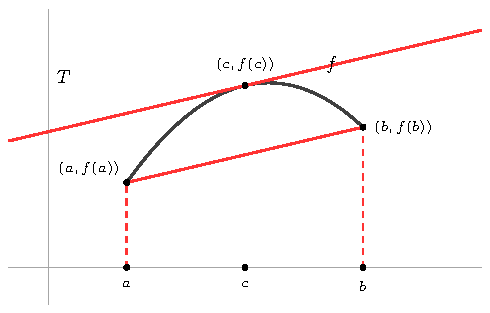
\includegraphics{figuras/valor-medio.pdf}
        \caption{Significado geométrico del teorema del valor medio. Existe $c\in(a,b)$ tal que
        la pendiente de la recta tangente $T$ a la gráfica de $f$ en el punto $(c,f(c))$ es la pendiente
        del segmento de recta que une a los puntos $(a,f(a))$ y $(b,f(b))$.}
        \label{fig:5.14}
    \end{figure}

    Para expresar el significado geométrico del teorema del valor medio generalizado
    consideremos la función $\sigma:[a,b]\to\R^{2}$ dada por
    \begin{equation*}
        \sigma(t)=(g(t),f(t)).
    \end{equation*}
    Cuando $t$ varía en el intervalo $[a,b]$ el punto $\sigma(t)$ describe una trayectoria en
    el plano que parte del punto $\sigma(a)=(g(a),f(a))$ y llega al punto $\sigma(b)=
    (g(b),f(b))$ (véase la figura~\ref{fig:5.15}). El significado geométrico del teorema del
    valor medio generalizado es que existe $c\in(a,b)$ tal que la recta tangente a
    la trayectoria que describe $\sigma(t)$ en el punto $\sigma(c)$\footnote{La definición precisa de la recta tangente a la trayectoria que describe $\sigma(t)$ en el punto
    $\sigma(c)=(g(c),f(c))$ se puede consultar en cualquier texto de cálculo diferencial de varias
    variables, por ejemplo, en \cite{nunez2020calculoIII}.} y el segmento de recta que
    une los puntos $\sigma(a)$ y $\sigma(b)$ tienen la misma pendiente.

    En las próximas secciones veremos el poder del teorema del valor medio,
    por lo pronto, en los ejercicios siguientes veremos una pequeña prueba de su
    utilidad.

    \begin{figure}[H]
        \centering
        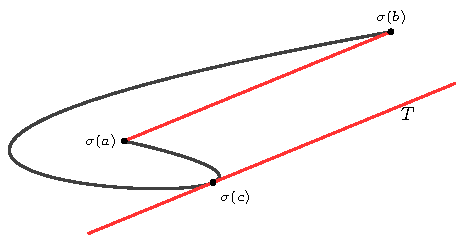
\includegraphics{figuras/valor-medio-generalizado.pdf}
        \caption{Significado geométrico del teorema del valor medio generalizado. Existe $c\in
        (a,b)$ tal que la pendiente de la recta tangente $T$ a la trayectoria que describe $\sigma(t)$ en el
        punto $\sigma(c)$ es la pendiente del segmento de recta que une a los puntos $\sigma(a)$ y $\sigma(b)$.}
        \label{fig:5.15}
    \end{figure}

    \par\avoidorphan{6}\subsection*{Ejercicios}

    \begin{ejercicio}\label{ej:267}
        Prueba que si $f:\R\to\R$ tiene derivada acotada, entonces es
        uniformemente continua.
    \end{ejercicio}

    El ejercicio siguiente nos ayudará en \cite{nunez2020calculoII} a probar la diferenciabilidad de
    las funciones trigonométricas.

    \begin{ejercicio}\label{ej:268}
        Sea $f$ una función continua en un intervalo $[a,b]$ (con $a<b$)
        que contiene a $p$. Prueba que si $f$ es derivable en $[a,b]\backslash\{p\}$\footnote{Que $f$ sea diferenciable en $[a,b]\backslash\{p\}$ significa que $f$ es diferenciable en $[a,p)$ y en $(p,b]$.} y $\lim_{x\to p}f'(x)$
        existe, entonces $f$ es derivable en $p$ y
        \begin{equation}\label{eq:5.24}
            f'(p)=\lim_{x\to p}f'(x)
        \end{equation}
        (si $p=a$ o $p=b$, el límite que aparece en \eqref{eq:5.24} se refiere a un límite lateral).
        \sugerencia Supón que $p\in(a,b)$, la demostración cuando $p=a$ o $p=b$
        es similar. Considera $h$ tal que $p+h\in[a,b]$. Por el teorema del valor medio
        existe $c_{h}$ entre $p$ y $p+h$ tal que
        \begin{equation*}
            f(p+h)-f(p)=f'(c_{h})h.
        \end{equation*}
        Prueba que $\lim_{h\to 0}f'(c_{h})=\lim_{x\to p}f'(x)$, de lo cual resulta que
        \begin{equation*}
            \lim_{h\to 0}\frac{f(p+h)-f(p)}{h}=\lim_{h\to 0}f'(c_{h})=\lim_{x\to p}f'(x).
        \end{equation*}
    \end{ejercicio}

    \section{Aplicaciones de la Derivada}\label{sec:aplicaciones-derivada}

    Estamos listos para ver el poder de la derivada. En esta sección utilizaremos
    los resultados que hemos obtenido sobre la derivada, entre ellos el
    teorema del valor medio, para analizar a una función. En las últimas dos
    subsecciones del capítulo aplicaremos todo lo obtenido para realizar análisis
    de gráficos y solucionar problemas de optimización.

    \subsection{Funciones Monótonas}\label{subsec:monotonas-derivada}

    Como consecuencia del teorema del valor medio obtenemos el corolario
    siguiente.

    \begin{corolario}\label{cor:2}
        Sea $f$ una función derivable en un intervalo abierto $I$. Se
        cumple lo siguiente:
        \begin{enumerate}[nosep]
            \item Si $f'(x)>0$ para toda $x$ en $I$, entonces $f$ es creciente en $I$.
            \item Si $f'(x)<0$ para toda $x$ en $I$, entonces $f$ es decreciente en $I$.
            \item Si $f'(x)=0$ para toda $x$ en $I$, entonces $f$ es constante en $I$.
        \end{enumerate}
    \end{corolario}

    \begin{proof}
        (a) Supongamos que $x,y\in I$ con $x<y$. Necesitamos probar
        que $f(x)<f(y)$. Por el teorema del valor medio sabemos que existe $c\in
        (x,y)$ tal que
        \begin{equation*}
            f(y)-f(x)=f'(c)(y-x).
        \end{equation*}
        Como $f'(c)>0$ y $y-x>0$, de la ecuación anterior obtenemos que $f(y)-
        f(x)>0$.

        (b) La prueba de esta afirmación es similar a la del inciso (a).

        (c) Supongamos que $x,y\in I$ con $x<y$. Necesitamos probar que $f(x)=
        f(y)$. Por el teorema del valor medio sabemos que existe $c\in(x,y)$ tal que
        \begin{equation*}
            f(y)-f(x)=f'(c)(y-x).
        \end{equation*}
        Como $f'(c)=0$, de la ecuación anterior obtenemos que $f(y)=f(x)$.
    \end{proof}

    De igual manera obtenemos el corolario siguiente.

    \begin{corolario}\label{cor:3}
        Sea $f$ una función derivable en un intervalo abierto $I$. Se
        cumple lo siguiente:
        \begin{enumerate}[nosep]
            \item Si $f'(x)\geq 0$ para toda $x$ en $I$, entonces $f$ es monótona creciente en $I$.
            \item Si $f'(x)\leq 0$ para toda $x$ en $I$, entonces $f$ es monótona decreciente en $I$.
        \end{enumerate}
    \end{corolario}

    Como aplicación de los corolarios~\ref{cor:2} y~\ref{cor:3} consideremos el ejemplo siguiente,
    el cual usamos en el ejemplo~\ref{ejm:53}.

    \begin{ejemplo}\label{ejm:89}
        Se cumple lo siguiente (véase la figura~\ref{fig:5.16}):
        \begin{enumerate}[nosep]
            \item $x\leq\sin(x)$ para todo $x\in(-\infty,0]$.
            \item $\sin(x)\leq x$ para todo $x\in[0,\infty)$.
            \item $\tan(x)\leq x$ para todo $x\in(-\pi/2,0]$.
            \item $x\leq\tan(x)$ para todo $x\in[0,\pi/2)$.
        \end{enumerate}
        En efecto, teniendo en cuenta el ejercicio~\ref{ej:108}, definamos
        \begin{equation*}
            f(x)=\sin(x)-x.
        \end{equation*}
        Como
        \begin{equation*}
            f'(x)=\cos(x)-1\leq 0,
        \end{equation*}
        entonces por el corolario~\ref{cor:3} obtenemos que $f$ es monótona decreciente en $\R$,
        por lo cual,
        \begin{equation*}
            \text{si }x\leq 0,\text{ entonces }f(x)\geq f(0)
        \end{equation*}
        y
        \begin{equation*}
            \text{si }0\leq x,\text{ entonces }f(0)\geq f(x),
        \end{equation*}
        de lo cual se siguen los incisos (a) y (b). La prueba de los incisos (c) y (d) es
        similar y se deja a cargo del lector (véase el ejercicio~\ref{ej:275}).
    \end{ejemplo}

    \begin{figure}[H]
        \centering
        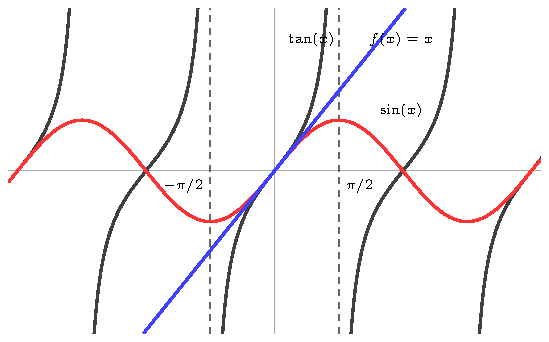
\includegraphics{figuras/seno-x-tangente.pdf}
        \caption{Gráficas de las funciones $\tan(x)$, $x$ y $\sin(x)$.}
        \label{fig:5.16}
    \end{figure}

    A continuación usaremos el corolario~\ref{cor:2} para determinar los intervalos abiertos
    donde una función $f$ es creciente o decreciente. En este tipo de problemas
    procederemos de la manera siguiente.

    \receta{\textbf{Receta para encontrar los intervalos abiertos donde una función} \normalfont$f$ (derivable en un intervalo abierto) \textbf{es creciente o decreciente:}\footnote{Usaremos este método para funciones con un conjunto finito de puntos críticos.}}\index{receta para encontrar los intervalos abiertos donde una funcion es creciente o decreciente@receta para encontrar los intervalos abiertos donde una función es creciente o decreciente}
    \begin{enumerate}[label=\arabic*.,nosep]
        \item Encontrar los puntos críticos de $f$.
        \item Considerar los intervalos abiertos determinados por los puntos críticos del
        inciso 1.\footnote{Por ejemplo, si $f$ está definida en $(a,b)$ y si $-2$, $5$ y $8$ son los puntos críticos de $f$ que
        están en $(a,b)$, entonces los intervalos abiertos generados por estos puntos críticos son los
        intervalos $(a,-2)$, $(-2,5)$, $(5,8)$ y $(8,b)$.}
        \item Determinar el signo de $f'$ en los intervalos del inciso 2.\footnote{Como el signo de $f'(x)$ es constante en cada uno de los intervalos del inciso 2 (¿por
        qué?), entonces para determinar el signo de la derivada en cada uno de esos intervalos
        basta tomar un punto de prueba $p$ en cada uno de ellos y ver el signo de $f'$ en $p$.}
        \item Usar el corolario~\ref{cor:2} en los intervalos del inciso 3 para determinar los intervalos
        abiertos donde $f$ es creciente o decreciente.
    \end{enumerate}

    \begin{ejemplo}\label{ejm:90}
        Encuentra los intervalos abiertos donde la función $f(x)=x^{3}+
        4x^{2}-3$ es creciente o decreciente.

        \textbf{Solución.} Seguiremos la receta anterior.
        \begin{enumerate}[label=\arabic*.]
            \item Encontrar los puntos críticos de $f$: Notemos que $f'(x)=3x^{2}+8x$. Así,
            \begin{align*}
                f'(x)=0&\Leftrightarrow 3x^{2}+8x=0\\
                &\Leftrightarrow x(3x+8)=0\\
                &\Leftrightarrow x=0\text{ o }x=-\frac{8}{3}.
            \end{align*}
            Por lo cual los puntos críticos de $f$ son $0$ y $-8/3$.
            \item Considerar los intervalos abiertos generados por los puntos críticos: $(-\infty,-8/3)$,
            $(-8/3,0)$ y $(0,\infty)$.
            \item Determinar el signo de $f'$ en los intervalos del inciso 2: Consideremos el
            esquema siguiente.
            \esquemasignos{f'}{$(-\infty,-8/3)$ & $-3$ & $+$ & $+$\\ \hline
            $(-8/3,0)$ & $-2$ & $-$ & $-$\\ \hline
            $(0,\infty)$ & $1$ & $+$ & $+$\\ \hline}
            \item Usar el corolario~\ref{cor:2}: $f$ es creciente en $(-\infty,-8/3)$, decreciente en $(-8/3,0)$
            y creciente en $(0,\infty)$. Véase la figura~\ref{fig:5.17}.\finej
        \end{enumerate}
    \end{ejemplo}

    \begin{figure}[H]
        \centering
        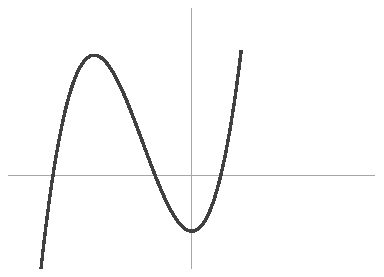
\includegraphics{figuras/cubica-crece.pdf}
        \caption{Gráfica de la función $f(x)=x^{3}+4x^{2}-3$}
        \label{fig:5.17}
    \end{figure}

    \subsection{Concavidad y Puntos de Inflexión}\label{subsec:concavidad}

    Supongamos que $f$ es una función derivable y creciente en un intervalo
    $(a,b)$. Entonces la gráfica de $f$ podría asemejar a un «puente», como la
    gráfica del inciso (a) de la figura~\ref{fig:5.18} o a un «columpio», como la gráfica del
    inciso (b) de la figura~\ref{fig:5.18} o una combinación de ellos, como la gráfica de la
    función $x^{3}$. Para estudiar de manera precisa este tipo de posibilidades sobre
    la gráfica de una función necesitamos primero el concepto de concavidad, el
    cual introduciremos después de la definición siguiente.

    \begin{figure}[H]
        \centering
        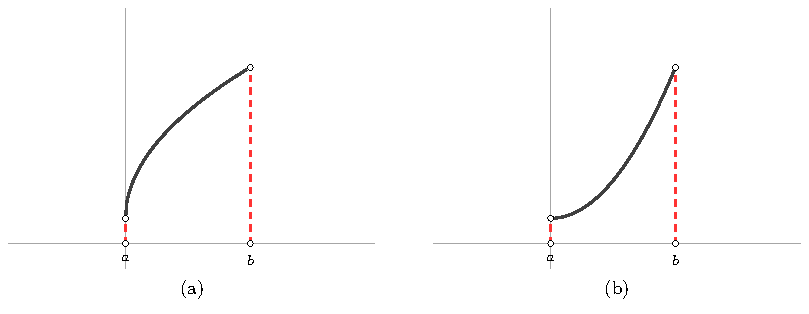
\includegraphics{figuras/concavidad-opciones.pdf}
        \caption{Dos posibles opciones para una función creciente en el intervalo $(a,b)$.}
        \label{fig:5.18}
    \end{figure}

    \begin{definicion}[Derivadas de orden superior]\label{def:52}
        \index{derivadas de orden superior}Sea $f$ una función definida
        en un intervalo abierto. Hemos denotado a la derivada de $f$ por $f'$. A la
        derivada de $f'$ la denotaremos por $f''$ y le llamaremos la \textit{segunda derivada}\index{segunda derivada}
        de $f$; a la derivada de $f''$ la denotaremos por $f'''$ y le llamaremos la tercera
        derivada de $f$, etc. Es costumbre ya no usar la notación con comas para
        denotar a la cuarta, quinta, sexta, etc., derivadas de $f$, pues esta notación
        se volvería inconveniente, en su lugar usaremos la siguiente: El símbolo $f^{(0)}$
        denotará a la función $f$ y le llamaremos la cero derivada de $f$; el símbolo
        $f^{(1)}$ denotará a la derivada de $f$ y le llamaremos la primera derivada de $f$; el
        símbolo $f^{(2)}$ denotará a la derivada de $f^{(1)}$ y le llamaremos la segunda derivada
        de $f$, etc. Notemos que con esta notación es más fácil expresar $f^{(20)}$ que
        $f''''''''''''''''''''$. Finalmente, diremos que $f$ es \textit{$n$-veces derivable}\index{funcion n-veces derivable@función $n$-veces derivable} en un punto $x$
        si existe $f^{(n)}(x)$ y diremos que $f$ es \textit{$n$-veces derivable} en un intervalo abierto
        $I$ si existe $f^{(n)}(x)$ para cada $x$ de $I$.
    \end{definicion}

    Ahora sí, definamos la concavidad.

    \begin{definicion}[Concavidad]\label{def:53}
        \index{concavidad}Sea $f$ una función definida en un intervalo
        abierto $I$.
        \begin{enumerate}[nosep]
            \item Diremos que $f$ es \textit{cóncava hacia abajo}\index{funcion concava hacia abajo@función cóncava hacia abajo} si $f''(x)<0$ para todo $x$ en $I$.
            \item Diremos que $f$ es \textit{cóncava hacia arriba}\index{funcion concava hacia arriba@función cóncava hacia arriba} si $f''(x)>0$ para todo $x$ en $I$.
        \end{enumerate}
    \end{definicion}

    De la definición~\ref{def:53} y del corolario~\ref{cor:2} obtenemos que una función cóncava
    hacia abajo en un intervalo abierto $I$ cumple que su derivada $f'$ es decreciente
    en $I$, y que una función cóncava hacia arriba en un intervalo abierto $I$ cumple
    que su derivada $f'$ es creciente en $I$. La gráfica de una función cóncava hacia
    abajo es como la gráfica del inciso (a) de la figura~\ref{fig:5.18} y la gráfica de una
    función cóncava hacia arriba es como la gráfica del inciso (b) de la misma
    figura.

    \begin{definicion}[Punto de inflexión]\label{def:54}
        Sea $f$ una función continua en un
        intervalo abierto que contiene a $p$. Diremos que $(p,f(p))$ es un \textit{punto de
        inflexión}\index{punto de inflexion@punto de inflexión} de la gráfica de $f$ si existen intervalos $(a,p)$ y $(p,b)$ tales que $f$
        tiene distinta concavidad en los intervalos $(a,p)$ y $(p,b)$.
    \end{definicion}

    Por ejemplo, el punto $(0,0)$ es un punto de inflexión de la gráfica de la
    función $f(x)=x^{3}$, pues $f$ es cóncava hacia abajo en el intervalo $(-\infty,0)$ y
    cóncava hacia arriba en el intervalo $(0,\infty)$ (véase la figura~\ref{fig:5.19}).

    \begin{figure}[H]
        \centering
        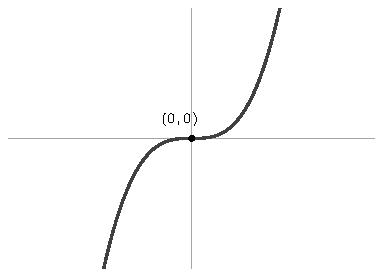
\includegraphics{figuras/inflexion-cubo.pdf}
        \caption{El punto $(0,0)$ es un punto de inflexión de la gráfica de la función $f(x)=x^{3}$.
        La concavidad de $f$ es diferente en los intervalos $(-\infty,0)$ y $(0,\infty)$.}
        \label{fig:5.19}
    \end{figure}

    Como otro ejemplo, el punto $(0,0)$ es un punto de inflexión de la gráfica de
    la función $f(x)=\sqrt[3]{x}$, pues $f$ es cóncava hacia arriba en el intervalo $(-\infty,0)$
    y cóncava hacia abajo en el intervalo $(0,\infty)$ (véase la figura~\ref{fig:5.20}).

    La proposición siguiente nos ayudará a encontrar los puntos de inflexión
    de la gráfica de una función.

    \begin{figure}[H]
        \centering
        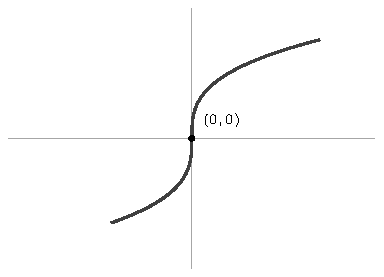
\includegraphics{figuras/inflexion-raiz-cubica.pdf}
        \caption{El punto $(0,0)$ es un punto de inflexión de la gráfica de la función $f(x)=\sqrt[3]{x}$.
        La concavidad de $f$ es diferente en los intervalos $(-\infty,0)$ y $(0,\infty)$.}
        \label{fig:5.20}
    \end{figure}

    \begin{proposicion}[Puntos de inflexión]\label{prop:64}
        Sea $f$ una función dos veces derivable
        en un intervalo abierto $I$ que contiene a $p$. Si $(p,f(p))$ es un punto
        de inflexión de la gráfica de $f$, entonces $f''(p)=0$.
    \end{proposicion}

    \begin{proof}
        Como $(p,f(p))$ es un punto de inflexión de la gráfica de $f$
        podemos suponer, sin pérdida de generalidad, que existen intervalos $(a,p)$ y
        $(p,b)$ tales que $f$ es cóncava hacia abajo en $(a,p)$ y cóncava hacia arriba en
        $(p,b)$. Así,
        \begin{equation}\label{eq:5.25}
            f''(x)<0\text{ en }(a,p)
        \end{equation}
        y
        \begin{equation}\label{eq:5.26}
            f''(x)>0\text{ en }(p,b).
        \end{equation}
        Tomemos $\alpha\in(a,p)$ y $\beta\in(p,b)$. Como $f''(\alpha)<0<f''(\beta)$, por el teorema
        del valor intermedio para derivadas (teorema~\ref{teo:6}), sabemos que existe $c\in(\alpha,\beta)$
        tal que $f''(c)=0$. De las ecuaciones \eqref{eq:5.25} y \eqref{eq:5.26} obtenemos que $c=p$,
        con lo cual obtenemos lo afirmado.
    \end{proof}

    El recíproco de la proposición anterior no es cierto, por ejemplo, si $f$ es
    una función constante, entonces $f''(0)=0$ y, sin embargo, $(0,f(0))$ no es un
    punto de inflexión de la gráfica de $f$.

    A continuación usaremos la proposición~\ref{prop:64} para determinar los intervalos
    abiertos donde una función $f$ (dos veces derivable en un intervalo abierto) es
    cóncava hacia arriba o cóncava hacia abajo, y para encontrar los puntos de
    inflexión de la gráfica de $f$, si existen. En este tipo de problemas procederemos
    de la manera siguiente.

    \receta{\textbf{Receta para encontrar los intervalos abiertos donde una función} \normalfont$f$ (dos veces derivable en un intervalo abierto) \textbf{es cóncava hacia arriba o cóncava hacia abajo, y para encontrar los puntos de inflexión:}\footnote{Usaremos este método para funciones tales que el conjunto $\{x:f''(x)=0\}$ es finito.}}\index{receta para encontrar los intervalos abiertos donde una funcion es concava hacia arriba o concava hacia abajo, y para encontrar los puntos de inflexion@receta para encontrar los intervalos abiertos donde una función es cóncava hacia arriba o cóncava hacia abajo, y para encontrar los puntos de inflexión}
    \begin{enumerate}[label=\arabic*.,nosep]
        \item Encontrar los puntos críticos de $f'$.
        \item Considerar los intervalos abiertos determinados por los puntos críticos del
        inciso 1.\footnote{Por ejemplo, si $f$ está definida en $(a,b)$ y si $-2$, $5$ y $8$ son los puntos críticos de $f'$ que
        están en $(a,b)$, entonces los intervalos generados por estos puntos críticos son los intervalos
        $(a,-2)$, $(-2,5)$, $(5,8)$ y $(8,b)$.}
        \item Determinar el signo de $f''$ en los intervalos del inciso 2.\footnote{Como el signo de $f''(x)$ es constante en cada uno de los intervalos del inciso 2 (¿por
        qué?), entonces para determinar el signo de la segunda derivada en cada uno de estos
        intervalos basta tomar un punto de prueba $p$ en cada uno de ellos y ver el signo de $f''$ en
        $p$.}
        \item Usar la información del inciso 3 para determinar los intervalos abiertos
        donde $f$ es cóncava hacia arriba y cóncava hacia abajo.
        \item Usar los intervalos encontrados en el inciso 4 para encontrar los puntos de
        inflexión de la gráfica de $f$, si existen.
    \end{enumerate}

    \begin{ejemplo}\label{ejm:91}
        Encuentra los intervalos abiertos donde la función $f(x)=x^{3}+
        4x^{2}-3$ es cóncava hacia arriba o cóncava hacia abajo, y los puntos de inflexión
        de la gráfica de $f$.

        \textbf{Solución.} Seguiremos la receta anterior.
        \begin{enumerate}[label=\arabic*.]
            \item Encontrar los puntos críticos de $f'$: Notemos que $f'(x)=3x^{2}+8x$ y que
            $f''(x)=6x+8$. Así,
            \begin{align*}
                f''(x)=0&\Leftrightarrow 6x+8=0\\
                &\Leftrightarrow x=-\frac{4}{3}.
            \end{align*}
            Por lo cual el punto crítico de $f'$ es $-4/3$.
            \item Considerar los intervalos abiertos determinados por los puntos críticos del
            inciso 1: $(-\infty,-4/3)$ y $(-4/3,\infty)$.
            \item Determinar el signo de $f''$ en los intervalos del inciso 2: Consideremos el
            esquema siguiente.
            \esquemasignos{f''}{$(-\infty,-4/3)$ & $-2$ & $-$ & $-$\\ \hline
            $(-4/3,\infty)$ & $0$ & $+$ & $+$\\ \hline}
            \item Usar la información del inciso 3 para determinar los intervalos abiertos
            donde $f$ es cóncava hacia arriba y cóncava hacia abajo: $f$ es cóncava hacia
            abajo en el intervalo $(-\infty,-4/3)$ y cóncava hacia arriba en el intervalo
            $(-4/3,\infty)$.
            \item Usar los intervalos encontrados en el inciso 4 para encontrar los puntos
            de inflexión de la gráfica de $f$: El punto de inflexión de la gráfica de $f$ es
            $(-4/3,f(-4/3))=(-4/3,47/27)$. Véase la figura~\ref{fig:5.21}.\finej
        \end{enumerate}
    \end{ejemplo}

    \begin{figure}[H]
        \centering
        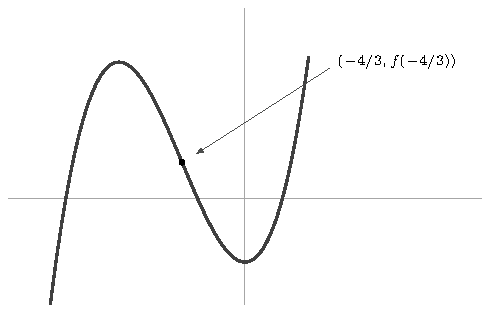
\includegraphics{figuras/cubica-inflexion.pdf}
        \caption{Gráfica de la función $f(x)=x^{3}+4x^{2}-3$}
        \label{fig:5.21}
    \end{figure}

    \subsection{Mínimos y Máximos Locales; Criterios de la Primera y Segunda Derivada}\label{subsec:criterios}

    Los dos criterios siguientes, consecuencias del teorema del valor medio o del
    corolario~\ref{cor:2}, serán la base fundamental para encontrar los mínimos y máximos
    locales, si existen, de una función.

    \begin{proposicion}[Criterio de la primera derivada]\label{prop:65}
        \index{criterio de la primera derivada}Sea $f$ una función
        continua en $p$.
        \begin{enumerate}[nosep]
            \item Si existe un intervalo abierto $(a,b)$ que contiene a $p$ tal que $f'(x)<0$ si
            $x\in(a,p)$ y $f'(x)>0$ si $x\in(p,b)$, entonces $f(p)$ es un mínimo local.
            \item Si existe un intervalo abierto $(a,b)$ que contiene a $p$ tal que $f'(x)>0$ si
            $x\in(a,p)$ y $f'(x)<0$ si $x\in(p,b)$, entonces $f(p)$ es un máximo local.
            \item Si existe un intervalo abierto $(a,b)$ que contiene a $p$ tal que $f'(x)>0$ si
            $x\in(a,p)$ y $f'(x)>0$ si $x\in(p,b)$, entonces $f(p)$ no es ni mínimo local
            ni máximo local.
            \item Si existe un intervalo abierto $(a,b)$ que contiene a $p$ tal que $f'(x)<0$ si
            $x\in(a,p)$ y $f'(x)<0$ si $x\in(p,b)$, entonces $f(p)$ no es ni mínimo local
            ni máximo local.
        \end{enumerate}
    \end{proposicion}

    \begin{proof}
        (a) Sea $x\in(a,b)$. Supongamos primero que $x<p$. Por el
        teorema del valor medio, existe $c\in(x,p)$ tal que
        \begin{equation}\label{eq:5.27}
            f(p)-f(x)=f'(c)(p-x).
        \end{equation}
        Como $f'(c)<0$, de \eqref{eq:5.27} obtenemos que $f(p)<f(x)$. De manera similar,
        si $x\in(a,b)$ y $p<x$ obtenemos que $f(p)<f(x)$. Por lo tanto, $f(p)$ es un
        mínimo local.

        (b) La prueba de esta afirmación es similar a la prueba del inciso (a).

        (c) Sea $x\in(a,b)$. Como en la prueba del inciso (a), si $x<p$ obtenemos
        que $f(x)<f(p)$, y si $p<x$ obtenemos que $f(p)<f(x)$. Por lo tanto, $f(p)$
        no es ni mínimo local ni máximo local.

        (d) La prueba de esta afirmación es similar a la prueba del inciso (c).
    \end{proof}

    ¿En qué parte de la demostración anterior se utilizó que $f$ es continua en
    $p$?

    El criterio de la primera derivada se aprecia mejor en el esquema de la
    figura~\ref{fig:5.22}.

    \begin{figure}[H]
        \centering
        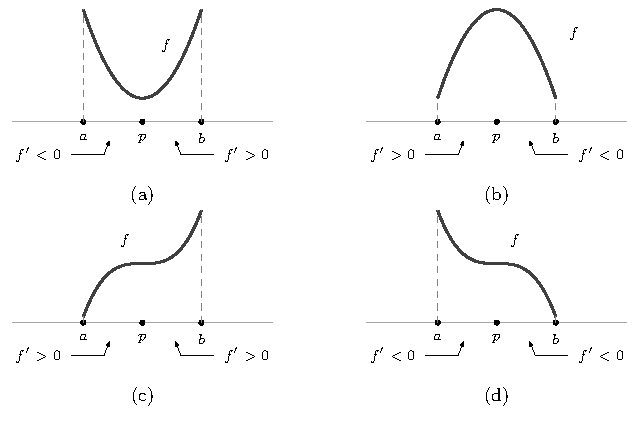
\includegraphics{figuras/criterio-primera.pdf}
        \caption{Esquema del criterio de la primera derivada. En el inciso (a) el número $f(p)$
        es un mínimo local, en el inciso (b) es un máximo local y en los incisos (c) y (d) no es ni
        mínimo local ni máximo local.}
        \label{fig:5.22}
    \end{figure}

    Ahora enunciamos el criterio de la segunda derivada.

    \begin{proposicion}[Criterio de la segunda derivada]\label{prop:66}
        \index{criterio de la segunda derivada}Sean $f$ una función
        dos veces derivable en un intervalo abierto $I$ y $p\in I$ un punto crítico de $f$.
        \begin{enumerate}[nosep]
            \item Si $f''(p)>0$, entonces $f(p)$ es un mínimo local.
            \item Si $f''(p)<0$, entonces $f(p)$ es un máximo local.
            \item Si $f''(p)=0$, entonces puede suceder que $f(p)$ sea mínimo local, máximo
            local o ninguna de las dos cosas.
        \end{enumerate}
    \end{proposicion}

    \begin{proof}
        (a) Como $f'(p)=0$, entonces
        \begin{align*}
            0<f''(p)&=\lim_{h\to 0}\frac{f'(p+h)-f'(p)}{h}\\
            &=\lim_{h\to 0}\frac{f'(p+h)}{h}.
        \end{align*}
        Así, existe $\delta>0$ tal que si $0<|h|<\delta$, entonces $f'(p+h)/h>0$. En
        consecuencia, si $0<|h|<\delta$ y $h<0$, entonces $f'(p+h)<0$. De manera
        similar, si $0<|h|<\delta$ y $h>0$, entonces $f'(p+h)>0$. En resumen, $f'(x)<0$
        si $x\in(p-\delta,p)$ y $f'(x)>0$ si $x\in(p,p+\delta)$. Luego, por el criterio de la
        primera derivada, $f(p)$ es un mínimo local.

        (b) La prueba de esta afirmación es similar a la del inciso (a).

        (c) Por ejemplo, si $f(x)=x^{4}$, $g(x)=-x^{4}$ y $r(x)=x^{3}$, entonces $0$ es un
        punto crítico de $f$, $g$ y $r$, $f''(0)=g''(0)=r''(0)=0$, $f(0)$ es un mínimo
        local de $f$, $g(0)$ es un máximo local de $g$ y $r(0)$ no es ni mínimo ni máximo
        local de $r$.
    \end{proof}

    A continuación, haciendo uso del criterio de la primera derivada, daremos
    una receta para determinar los mínimos y máximos locales de una función
    $f$. En esta receta no usamos el criterio de la segunda derivada, pues pueden
    existir puntos críticos de $f$ en los que el criterio de la segunda derivada no
    da información (por supuesto, el lector puede usar el criterio de la segunda
    derivada en los puntos críticos donde sea concluyente).

    \receta{\textbf{Receta para encontrar los mínimos locales y máximos locales de una función} \normalfont$f$ (derivable en un intervalo abierto) \textbf{(utilizando el criterio de la primera derivada):}\footnote{Usaremos este método para funciones con un conjunto finito de puntos críticos.}}\index{receta para encontrar los minimos locales y maximos locales de una funcion@receta para encontrar los mínimos locales y máximos locales de una función}
    \begin{enumerate}[label=\arabic*.,nosep]
        \item Encontrar los puntos críticos de $f$.
        \item Considerar los intervalos abiertos determinados por los puntos críticos del
        inciso 1.\footnote{Por ejemplo, si $f$ está definida en $(a,b)$ y si $-2$, $5$ y $8$ son los puntos críticos de $f$ que
        están en $(a,b)$, entonces los intervalos abiertos generados por estos puntos críticos son los
        intervalos $(a,-2)$, $(-2,5)$, $(5,8)$ y $(8,b)$.}
        \item Determinar el signo de $f'$ en los intervalos del inciso 2.\footnote{Como el signo de $f'(x)$ es constante en cada uno de los intervalos del inciso 2 (¿por
        qué?), entonces para determinar el signo de la derivada en cada uno de estos intervalos
        basta tomar un punto de prueba $p$ en cada uno de ellos y ver el signo de $f'$ en $p$.}
        \item Aplicar el criterio de la primera derivada a los puntos críticos del inciso 1
        usando los intervalos del inciso 2 y la información del inciso 3.
    \end{enumerate}

    Notemos que, por la proposición~\ref{prop:63}, con el proceso anterior se encuentran
    todos los mínimos locales y máximos locales de $f$.

    \begin{ejemplo}\label{ejm:92}
        Encuentra los mínimos locales y máximos locales de la función
        \begin{equation*}
            f(x)=\frac{1}{5}x^{5}-\frac{4}{3}x^{3}.
        \end{equation*}

        \textbf{Solución.} Seguiremos la receta anterior.
        \begin{enumerate}[label=\arabic*.]
            \item Encontrar los puntos críticos de $f$: Como
            \begin{equation*}
                f'(x)=x^{4}-4x^{2}=x^{2}\left(x^{2}-4\right),
            \end{equation*}
            entonces los puntos críticos de $f$ son $-2$, $0$ y $2$.
            \item Considerar los intervalos abiertos determinados por los puntos críticos del
            inciso 1: $(-\infty,-2)$, $(-2,0)$, $(0,2)$ y $(2,\infty)$.
            \item Determinar el signo de $f'$ en los intervalos del inciso 2: Procederemos como
            en el ejemplo~\ref{ejm:90}. Consideremos el esquema siguiente.
            \esquemasignos{f'}{$(-\infty,-2)$ & $-3$ & $+$ & $+$\\ \hline
            $(-2,0)$ & $-1$ & $-$ & $-$\\ \hline
            $(0,2)$ & $1$ & $-$ & $-$\\ \hline
            $(2,\infty)$ & $3$ & $+$ & $+$\\ \hline}
            Así, $f'>0$ en $(-\infty,-2)$, $f'<0$ en $(-2,0)$, $f'<0$ en $(0,2)$ y $f'>0$ en
            $(2,\infty)$.
            \item Aplicar el criterio de la primera derivada a los puntos críticos del inciso
            1 usando los intervalos del inciso 2 y la información del inciso 3: Por el
            criterio de la primera derivada, $f(-2)$ es un máximo local, $f(0)$ no es ni
            mínimo ni máximo local y $f(2)$ es un mínimo local. Véase la figura~\ref{fig:5.23}.\finej
        \end{enumerate}
    \end{ejemplo}

    \begin{figure}[H]
        \centering
        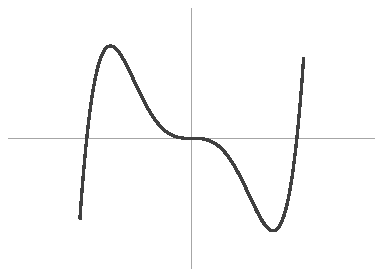
\includegraphics{figuras/quintica.pdf}
        \caption{Gráfica de la función $f(x)=\frac{1}{5}x^{5}-\frac{4}{3}x^{3}$.}
        \label{fig:5.23}
    \end{figure}

    Notemos que en el ejemplo anterior no podemos aplicar el criterio de la
    segunda derivada al punto crítico $0$, pues $f''(0)=0$. Por otra parte, puesto
    que $f''(-2)=-16<0$ y $f''(2)=16>0$, entonces por el criterio de
    la segunda derivada tenemos que $f(-2)$ es un máximo local y $f(2)$ es un
    mínimo local, como ya lo sabíamos.

    Si se puede aplicar el criterio de la segunda derivada a todos los puntos
    críticos de $f$ y resulta que evaluar $f''$ en tales puntos críticos es sencillo, el
    lector puede optar por usar el criterio de la segunda derivada en lugar de la
    receta dada para encontrar los mínimos y máximos locales.

    \begin{ejemplo}\label{ejm:93}
        Encuentra los mínimos locales y máximos locales de la función
        $f(x)=x^{4}-2x^{2}+1$ utilizando el criterio de la segunda derivada.

        \textbf{Solución.} Como $f'(x)=4x^{3}-4x=4x\left(x^{2}-1\right)$, los puntos críticos de
        $f$ son $-1$, $0$ y $1$. Como $f''(x)=\left(4x^{3}-4x\right)'=12x^{2}-4$, entonces
        \begin{equation*}
            f''(-1)=8>0,\ \ f''(0)=-4<0,\ \text{ y }\ f''(1)=8>0,
        \end{equation*}
        así, por el criterio de la segunda derivada, $f(-1)=0$ es un mínimo local,
        $f(0)=1$ es un máximo local y $f(1)=0$ es un mínimo local (véase la figura~\ref{fig:5.24}).
    \end{ejemplo}

    \begin{figure}[H]
        \centering
        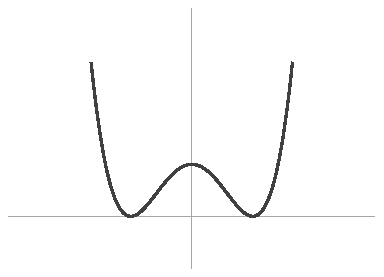
\includegraphics{figuras/cuartica-w.pdf}
        \caption{Gráfica de la función $f(x)=x^{4}-2x^{2}+1$.}
        \label{fig:5.24}
    \end{figure}

    \subsection{Mínimos y Máximos Globales}

    Ahora encontraremos el mínimo global y el máximo global de una función
    continua $f$ definida en un intervalo cerrado $[a,b]$. Por el teorema del mínimo y
    del máximo (teorema~\ref{teo:2}) sabemos que $f$ tiene un mínimo global y un máximo
    global, para encontrarlos seguiremos la receta siguiente.

    \receta{\textbf{Receta para encontrar los mínimos y máximos globales de una función continua} $\boldsymbol{f}$ \textbf{definida en un intervalo cerrado} $\boldsymbol{[a,b]}$\textbf{:}}\index{receta para encontrar los minimos y maximos globales de una funcion continua definida en un intervalo cerrado [a,b]@receta para encontrar los mínimos y máximos globales de una función continua definida en un intervalo cerrado $[a,b]$}
    \begin{enumerate}[label=\arabic*.,nosep]
        \item Encontrar los mínimos locales y máximos locales de $f$ en el intervalo $(a,b)$.
        \item El mínimo global de $f$ será el mínimo de los valores de $f(a)$, $f(b)$ y los
        mínimos locales de $f$. El máximo global de $f$ será el máximo de los valores
        de $f(a)$, $f(b)$ y los máximos locales de $f$.
    \end{enumerate}

    \begin{ejemplo}\label{ejm:94}
        Encuentra el mínimo global y el máximo global de la función
        $f(x)=x^{3}-3x$ en el intervalo $\left[-\sqrt{3},5/2\right]$.

        \textbf{Solución.} Seguiremos la receta anterior.
        \begin{enumerate}[label=\arabic*.]
            \item Encontrar los mínimos locales y máximos locales de $f$ en el intervalo
            $\left(-\sqrt{3},5/2\right)$: Como $f'(x)=3x^{2}-3$, los puntos críticos de $f$ son $-1$ y $1$; y
            ambos están en $\left(-\sqrt{3},5/2\right)$. Puesto que $f''(x)=6x$, entonces $f''(-1)<0$
            y $f''(1)>0$. Luego, por el criterio de la segunda derivada tenemos que
            $f(-1)=2$ es un máximo local y que $f(1)=-2$ es un mínimo local.
            \item El mínimo global de $f$ es
            \begin{equation*}
                \min\left\{f\left(-\sqrt{3}\right),f(5/2),f(1)\right\}=f(1)=-2
            \end{equation*}
            y el máximo global de $f$ es
            \begin{equation*}
                \max\left\{f\left(-\sqrt{3}\right),f(5/2),f(-1)\right\}=f(5/2)=65/8
            \end{equation*}
            (véase la figura~\ref{fig:5.25}).\finej
        \end{enumerate}
    \end{ejemplo}

    \begin{figure}[H]
        \centering
        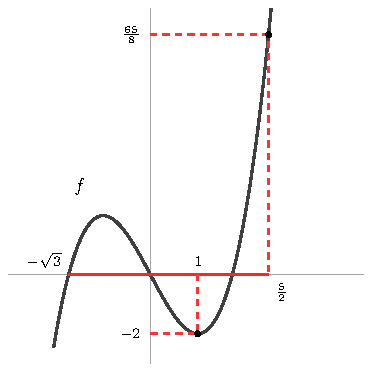
\includegraphics{figuras/extremos-globales-cubica.pdf}
        \caption{Gráfica de la función $f(x)=x^{3}-3x$. El mínimo global y máximo global de
        $f$ en el intervalo $\left[-\sqrt{3},5/2\right]$ son $f(1)=-2$ y $f(5/2)=65/8$, respectivamente.}
        \label{fig:5.25}
    \end{figure}

    \begin{ejemplo}\label{ejm:95}
        Encuentra el mínimo global y el máximo global de la función
        \begin{equation*}
            f(x)=\frac{1}{4}x^{4}-\frac{1}{3}x^{3}-x^{2}
        \end{equation*}
        en el intervalo $[-1/2,5/2]$.

        \textbf{Solución.} Seguiremos la receta anterior.
        \begin{enumerate}[label=\arabic*.]
            \item Encontrar los mínimos locales y máximos locales de $f$ en el intervalo
            $(-1/2,5/2)$: Como $f'(x)=x^{3}-x^{2}-2x=x(x-2)(x+1)$, los puntos
            críticos de $f$ son $-1$, $0$ y $2$. Solo consideraremos los puntos críticos $0$
            y $2$, pues $-1\notin(-1/2,5/2)$. Puesto que $f''(x)=3x^{2}-2x-2$, entonces
            $f''(0)<0$ y $f''(2)>0$. Luego, por el criterio de la segunda derivada
            tenemos que $f(0)=0$ es un máximo local y que $f(2)=-8/3$ es un mínimo
            local.
            \item El mínimo global de $f$ es
            \begin{equation*}
                \min\{f(-1/2),f(5/2),f(2)\}=f(2)=-\frac{8}{3}
            \end{equation*}
            y el máximo global de $f$ es
            \begin{equation*}
                \max\{f(-1/2),f(5/2),f(0)\}=f(0)=0
            \end{equation*}
            (véase la figura~\ref{fig:5.26}).\finej
        \end{enumerate}
    \end{ejemplo}

    \begin{figure}[H]
        \centering
        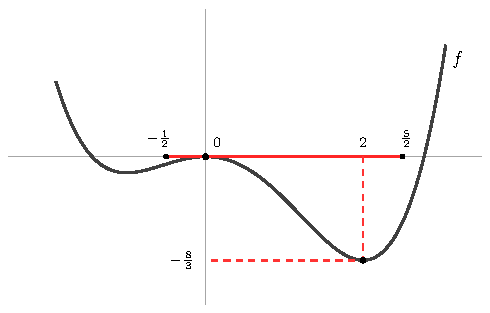
\includegraphics{figuras/extremos-globales-cuartica.pdf}
        \caption{Gráfica de la función $f(x)=\frac{1}{4}x^{4}-\frac{1}{3}x^{3}-x^{2}$. El mínimo global y el máximo
        global de $f$ en el intervalo $[-1/2,5/2]$ son $f(2)=-8/3$ y $f(0)=0$, respectivamente.}
        \label{fig:5.26}
    \end{figure}

    \subsection{Análisis de Gráficos}\label{subsec:graficos}

    En esta subsección aplicaremos todo lo aprendido en las subsecciones anteriores
    para analizar el comportamiento de una función a través de su gráfica.
    En general, para estudiar la gráfica de una función seguiremos el procedimiento
    siguiente.

    \receta{\textbf{Procedimiento para analizar la gráfica de una función} $\boldsymbol{f}$\textbf{:}}\index{procedimiento para analizar la grafica de una funcion@procedimiento para analizar la gráfica de una función}
    \begin{enumerate}[label=\arabic*.,nosep]
        \item Determinar el dominio de $f$.
        \item Determinar las intersecciones de la gráfica de $f$ con los ejes coordenados.
        \item Determina si $f$ es par o impar.
        \item Determinar los intervalos abiertos donde $f$ es creciente o decreciente.
        \item Determinar los intervalos abiertos donde $f$ es cóncava hacia arriba o hacia
        abajo.
        \item Determinar los puntos de inflexión de la gráfica de $f$.
        \item Determinar los mínimos locales y máximos locales de $f$.
        \item Determinar el mínimo global y el máximo global de $f$.
        \item Determinar las asíntotas de la gráfica de $f$.
        \item Trazar la gráfica de $f$.
    \end{enumerate}

    \begin{ejemplo}\label{ejm:96}
        Analiza la gráfica de la función $f(x)=6x^{5}-10x^{3}$.

        \textbf{Solución.} Emplearemos el procedimiento anterior para realizar el análisis.
        \begin{enumerate}[label=\arabic*.]
            \item Determinar el dominio de $f$: Como $f$ es un polinomio, entonces su dominio
            es todo $\R$.
            \item Determinar las intersecciones de la gráfica de $f$ con los ejes coordenados:
            Las intersecciones de la gráfica de $f$ con el eje $X$ son los puntos de la forma
            $(x,f(x))$, con $f(x)=0$. Como
            \begin{align*}
                &f(x)=0\\
                \Leftrightarrow{}&6x^{5}-10x^{3}=0\\
                \Leftrightarrow{}&2x^{3}\left(3x^{2}-5\right)=0\\
                \Leftrightarrow{}&x=0,\ \ x=\frac{\sqrt{5}}{\sqrt{3}}\text{ o }x=-\frac{\sqrt{5}}{\sqrt{3}},
            \end{align*}
            entonces las intersecciones de la gráfica de $f$ con el eje $X$ son los puntos
            $\left(-\sqrt{5}/\sqrt{3},0\right)$, $(0,0)$ y $\left(\sqrt{5}/\sqrt{3},0\right)$. Por otra parte, la intersección de la
            gráfica de $f$ con el eje $Y$ es el punto $(0,f(0))=(0,0)$.
            \item Determina si $f$ es par o impar: Como $f(-x)=-f(x)$ para todo $x$, entonces
            $f$ es impar. Por otra parte, puesto que $f(-1)=4\neq -4=f(1)$,
            entonces $f$ no es par.
            \item Determinar los intervalos abiertos donde $f$ es creciente o decreciente: Como
            \begin{align*}
                &f'(x)=0\\
                \Leftrightarrow{}&30x^{4}-30x^{2}=0\\
                \Leftrightarrow{}&x^{2}\left(x^{2}-1\right)=0\\
                \Leftrightarrow{}&x=0,\ \ x=1\text{ o }x=-1,
            \end{align*}
            entonces los puntos críticos de $f$ son $-1$, $0$ y $1$. Para encontrar los
            intervalos abiertos donde $f$ es creciente o decreciente consideremos el esquema
            siguiente.
            \esquemasignos{f'}{$(-\infty,-1)$ & $-3$ & $+$ & $+$\\ \hline
            $(-1,0)$ & $-1/2$ & $-$ & $-$\\ \hline
            $(0,1)$ & $1/2$ & $-$ & $-$\\ \hline
            $(1,\infty)$ & $2$ & $+$ & $+$\\ \hline}
            Así, $f$ es creciente en $(-\infty,-1)$, decreciente en $(-1,0)$, decreciente en
            $(0,1)$ y creciente en $(1,\infty)$.
            \item Determinar los intervalos donde $f$ es cóncava hacia arriba o hacia abajo:
            Como
            \begin{align*}
                &f''(x)=0\\
                \Leftrightarrow{}&120x^{3}-60x=0\\
                \Leftrightarrow{}&60x\left(2x^{2}-1\right)=0\\
                \Leftrightarrow{}&x=0,\ \ x=\frac{1}{\sqrt{2}}\text{ o }x=-\frac{1}{\sqrt{2}},
            \end{align*}
            entonces los puntos críticos de $f'$ son $-1/\sqrt{2}$, $0$ y $1/\sqrt{2}$. Para encontrar los
            intervalos abiertos donde $f$ es cóncava hacia arriba o cóncava hacia abajo
            consideremos el esquema siguiente.
            \esquemasignos{f''}{$\left(-\infty,-1/\sqrt{2}\right)$ & $-1$ & $-$ & $-$\\ \hline
            $\left(-1/\sqrt{2},0\right)$ & $-1/2$ & $+$ & $+$\\ \hline
            $\left(0,1/\sqrt{2}\right)$ & $1/2$ & $-$ & $-$\\ \hline
            $\left(1/\sqrt{2},\infty\right)$ & $1$ & $+$ & $+$\\ \hline}
            Así, $f$ es cóncava hacia abajo en $\left(-\infty,-1/\sqrt{2}\right)$, cóncava hacia arriba en
            $\left(-1/\sqrt{2},0\right)$, cóncava hacia abajo en $\left(0,1/\sqrt{2}\right)$ y cóncava hacia arriba en
            $\left(1/\sqrt{2},\infty\right)$.
            \item Determinar los puntos de inflexión de la gráfica de $f$: Del inciso 5, obtenemos
            que los puntos $\left(-1/\sqrt{2},f\left(-1/\sqrt{2}\right)\right)=\left(-1/\sqrt{2},7/2\sqrt{2}\right)$, $(0,f(0))=
            (0,0)$ y $\left(1/\sqrt{2},f\left(1/\sqrt{2}\right)\right)=\left(1/\sqrt{2},-7/2\sqrt{2}\right)$ son los puntos de inflexión
            de la gráfica de $f$.
            \item Determinar los mínimos locales y máximos locales de $f$: Utilizando la
            información del paso 3, por el criterio de la primera derivada sabemos que
            $f(-1)=4$ es un máximo local, $f(1)=-4$ es un mínimo local y $f(0)$ no
            es ni mínimo local ni máximo local.
            \item Determinar el mínimo global y el máximo global de $f$: En este caso no hay
            ni mínimo global ni máximo global, pues por la proposición~\ref{prop:52} tenemos
            que $\lim_{x\to-\infty}f(x)=-\infty$ y $\lim_{x\to\infty}f(x)=\infty$.
            \item Determinar las asíntotas de la gráfica de $f$: Como $\lim_{x\to\pm\infty}f(x)=\pm\infty$
            no es un número real, entonces la gráfica de $f$ no tiene asíntotas horizontales.
            Por otra parte, puesto que $\lim_{x\to p}f(x)=f(p)\neq\pm\infty$, entonces
            la gráfica de $f$ no tiene asíntotas verticales. Finalmente, la gráfica de $f$
            tampoco tiene asíntotas oblicuas, pues si $l(x)$ es un polinomio de grado
            $1$, entonces $\lim_{x\to\pm\infty}f(x)-l(x)=\pm\infty\neq 0$.
            \item Trazar la gráfica de $f$: La gráfica de $f$ aparece en la figura~\ref{fig:5.27}.\finej
        \end{enumerate}
    \end{ejemplo}

    \begin{figure}[H]
        \centering
        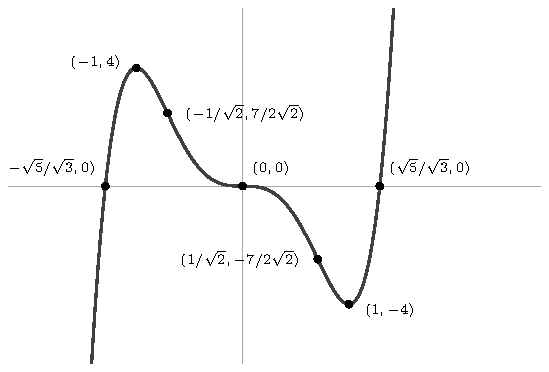
\includegraphics{figuras/analisis-quintica.pdf}
        \caption{Gráfica de $f(x)=6x^{5}-10x^{3}$.}
        \label{fig:5.27}
    \end{figure}

    \subsection{Problemas de Optimización}

    Ahora veremos algunos ejemplos clásicos de optimización en donde aplicaremos
    las técnicas aprendidas en esta sección. Optimizar un proceso es
    importante en la ciencia y en la industria, por ejemplo, en la industria es
    importante minimizar los costos y al mismo tiempo maximizar los beneficios
    de la producción de un artículo.

    \begin{ejemplo}[Caja óptima]\label{ejm:97}
        Supongamos que un fabricante de empaques
        tiene un pedido de cajas de metal sin tapa y base cuadrada para un cliente.
        El cliente requiere que cada caja tenga un volumen $V$ de $256$ cm$^{3}$. ¿Cuáles
        serán las dimensiones de la caja que minimicen la cantidad de metal para
        construirla?

        \textbf{Solución.} Sea $S$ la superficie de una caja de volumen $V=256$ cm$^{3}$.
        Deseamos encontrar las dimensiones de la caja de manera que su superficie
        $S$ sea mínima. Sean $x$, $y$ y $z$ las dimensiones de la caja (véase la figura~\ref{fig:5.28}).
        Como la base de la caja es cuadrada, entonces $y=x$ y puesto que se requiere
        que la caja tenga un volumen de $256$ cm$^{3}$, entonces
        \begin{equation}\label{eq:5.28}
            256=V=x^{2}z.
        \end{equation}
        Por otra parte, la superficie de la caja es
        \begin{equation}\label{eq:5.29}
            S=x^{2}+4xz.
        \end{equation}
        De la ecuación \eqref{eq:5.28} despejamos $z$ y la sustituimos en la ecuación \eqref{eq:5.29}
        para obtener la ecuación
        \begin{align*}
            S&=x^{2}+4xz\\
            &=x^{2}+4x\left(\frac{256}{x^{2}}\right)\\
            &=x^{2}+\frac{1024}{x}.
        \end{align*}
        Como la caja debe tener volumen ($V=256>0$), entonces solo consideraremos
        $x>0$, es decir, supondremos que el dominio de $S$ es el intervalo
        $(0,\infty)$. Encontrar las dimensiones de la caja que minimicen la cantidad de
        metal para construirla equivale a encontrar el mínimo global de la función
        $S$ en el intervalo $(0,\infty)$; si encontramos que $S(p)$ es el mínimo global de $S$
        en $(0,\infty)$, entonces las dimensiones de la caja que minimizan la cantidad de
        metal para construirla son $x=y=p$ y $z=256/x^{2}=256/p^{2}$.

        Dado que $S'(x)=2x-1024/x^{2}$, entonces el único punto crítico de $S$ es $8$,
        que está en $(0,\infty)$. Puesto que $S''(x)=2+2048/x^{3}$, entonces $S''(8)=6>0$.
        Así, por el criterio de la segunda derivada, $S(8)$ es un mínimo local, de
        hecho, puesto que $S$ es decreciente en $(0,8)$ y creciente en $(8,\infty)$ (¿por qué?),
        entonces $S(8)$ es el mínimo global de $S$.\footnote{Podemos mostrar que $S(8)$ es el mínimo global de $S$ de varias maneras (utilizando
        los resultados de esta sección) y no solo la que hemos expuesto. Por ejemplo, también
        podemos asegurar que $S(8)$ es el mínimo global de $S$ a partir del que $\lim_{x\to 0^{+}}S(x)=
        \lim_{x\to\infty}S(x)=\infty$.} En consecuencia, las dimensiones
        de la caja buscada son $x=y=8$ cm y $z=256/x^{2}=256/64=4$ cm; y la
        superficie mínima de la caja es $S(8)=192$ cm$^{2}$.
    \end{ejemplo}

    \begin{figure}[H]
        \centering
        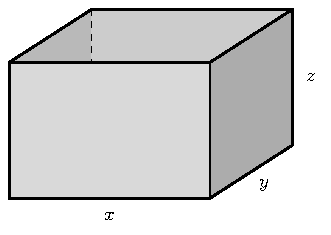
\includegraphics{figuras/caja.pdf}
        \caption{Caja de dimensiones $x$, $y$ y $z$.}
        \label{fig:5.28}
    \end{figure}

    Para apreciar la importancia de optimizar un proceso, supongamos que en
    el ejemplo anterior el cliente pide $10$ millones de cajas y que el costo del metal
    empleado para construir la caja es de $2$ pesos cada decímetro cuadrado. Si
    por un mal diseño de la caja se emplean $193$ cm$^{2}$ en cada caja, ¿cuál será la
    pérdida de capital en la construcción de los $10$ millones de cajas? Sabemos
    que el costo por cm$^{2}$ de metal es $0.02$ pesos, luego, si por el mal diseño de la
    caja se empleó un cm$^{2}$ de metal de más en cada caja, la pérdida de capital
    en la construcción de los $10$ millones de cajas será de $200000.00$ pesos, ¡Ups!

    En general, para resolver problemas de optimización como el del ejemplo
    anterior, se sigue la estrategia siguiente.

    \receta{\textbf{Estrategia general para resolver problemas de optimización:}}\index{estrategia para resolver problemas de optimizacion@estrategia para resolver problemas de optimización}
    \begin{enumerate}[label=\arabic*.,nosep]
        \item Determinar la propiedad (longitud, área, volumen, temperatura, pérdida,
        ganancia, costo, beneficio, etc) que se quiere optimizar (minimizar o
        maximizar).
        \item Determinar las variables, constantes y condiciones dadas en el problema.
        \item Introducir una función $f$ que represente la propiedad que se quiere optimizar.
        Por lo general esta función depende de varias variables.
        \item Utilizando las condiciones del problema, transformar la función $f$ en una
        función de una variable.
        \item Definir el dominio de la función $f$ de manera que el problema tenga sentido.
        \item Encontrar el mínimo global o el máximo global de la función $f$ (dependiendo
        de lo que pida el problema) y dónde se alcanza.
    \end{enumerate}

    Para mostrar el uso de esta estrategia para resolver problemas de optimización
    veamos el ejemplo siguiente.

    \begin{ejemplo}\label{ejm:98}
        Muestra que el rectángulo de mayor área inscrito en un círculo
        dado es un cuadrado.

        \textbf{Solución.} Emplearemos la estrategia anterior para mostrar lo afirmado.
        Por sencillez supondremos que el círculo dado está centrado en el origen y
        que el rectángulo buscado tiene lados paralelos a los ejes coordenados.
        \begin{enumerate}[label=\arabic*.]
            \item Determinar la propiedad que se quiere optimizar: Sea $A$ el área de un
            rectángulo $R$ inscrito en un círculo de radio $r$. Por sencillez supondremos
            que el círculo está centrado en el origen (véase la figura~\ref{fig:5.29}). Deseamos
            encontrar las dimensiones del rectángulo $R$ de manera que su área $A$ sea
            máxima.
            \item Determinar las variables, constantes y condiciones dadas en el problema:
            Sean $x$ y $y$ las longitudes de los lados del rectángulo $R$. Así, $(x/2)^{2}+
            (y/2)^{2}=r^{2}$.
            \item Introducir una función que represente la propiedad que se quiere optimizar:
            El área $A$ del rectángulo $R$ es $A=xy$.
            \item Utilizando las condiciones del problema, transformar la función $A$ en
            una función de una variable: Como $x^{2}/4+y^{2}/4=r^{2}$, entonces $y=
            2\sqrt{r^{2}-x^{2}/4}$ y, en consecuencia,
            \begin{align*}
                A&=xy\\
                &=2x\sqrt{r^{2}-\frac{x^{2}}{4}}.
            \end{align*}
            \item Definir el dominio de la función $A$ de manera que el problema tenga sentido:
            Como el rectángulo $R$ está inscrito en un círculo de radio $r$, entonces
            solo consideraremos $x$ con $0<x<2r$, es decir, supondremos que el dominio
            de $A$ es el intervalo $(0,2r)$.
            \item Encontrar el máximo global de la función $A$ y dónde se alcanza: Como las
            $x$ en el dominio de $A$ son positivas, entonces $A(x)=\sqrt{4x^{2}r^{2}-x^{4}}$. Para
            encontrar el máximo global de $A$ y dónde se alcanza notemos que si $f$ es
            una función no negativa, entonces la función $\sqrt{f(x)}$ alcanza un mínimo
            (máximo) en un número $p$ ssi $f$ alcanza un mínimo (máximo) en $p$; esto
            se debe a que las funciones $x^{2}$ y $\sqrt{x}$ son crecientes en el intervalo $[0,\infty)$;
            en consecuencia, para encontrar dónde se alcanza el máximo global de la
            función $A$ basta encontrar dónde se alcanza el máximo global de la función
            $f(x)=4x^{2}r^{2}-x^{4}$. Como $f'(x)=8xr^{2}-4x^{3}$, entonces el único punto
            crítico de $f$ es $\sqrt{2}r$, que está en $(0,2r)$. Puesto que $f''(x)=8r^{2}-12x^{2}$,
            entonces $f''\left(\sqrt{2}r\right)=-16r^{2}<0$. Así, por el criterio de la segunda derivada,
            $f\left(\sqrt{2}r\right)$ es un máximo local de $f$. De hecho, puesto que $f$ es creciente
            en $\left(0,\sqrt{2}r\right)$ y decreciente en $\left(\sqrt{2}r,2r\right)$ (¿por qué?), entonces $f\left(\sqrt{2}r\right)$ es el
            máximo global de $f$. Por lo comentado anteriormente $A\left(\sqrt{2}r\right)$ es el máximo
            global de la función $A$. En consecuencia, las dimensiones del rectángulo
            buscado son $x=\sqrt{2}r$ y $y=2\sqrt{r^{2}-x^{2}/4}=\sqrt{2}r$. Así, $R$ es un cuadrado.\finej
        \end{enumerate}
    \end{ejemplo}

    \begin{figure}[H]
        \centering
        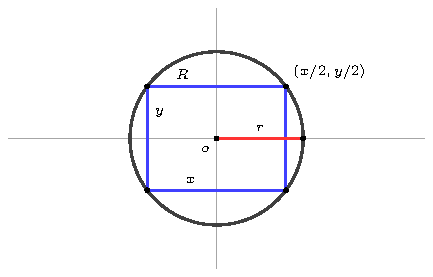
\includegraphics{figuras/rectangulo-inscrito.pdf}
        \caption{Rectángulo de dimensiones $x$ y $y$ inscrito en una circunferencia de radio
        $r$.}
        \label{fig:5.29}
    \end{figure}

    \par\avoidorphan{6}\subsection*{Ejercicios}

    \subtitulo{Funciones Monótonas}

    \begin{ejercicio}\label{ej:269}
        Construye la gráfica de una función cuya derivada siempre
        sea positiva.
    \end{ejercicio}

    \begin{ejercicio}\label{ej:270}
        Construye la gráfica de una función cuya derivada siempre
        sea negativa.
    \end{ejercicio}

    Los dos ejercicios siguientes son los ejercicios~\ref{ej:59} y~\ref{ej:60} de la sección~\ref{sec:naturales},
    respectivamente; es instructivo probarlos ahora utilizando los resultados de
    la subsección~\ref{subsec:monotonas-derivada}.

    \begin{ejercicio}\label{ej:271}
        Sea $n$ un número natural.
        \begin{enumerate}[nosep]
            \item Prueba, utilizando los resultados de la subsección~\ref{subsec:monotonas-derivada}, que si $n$ es par,
            entonces la función $x^{n}$ es decreciente en $(-\infty,0]$ y creciente en $[0,\infty)$.
            \item Prueba, utilizando los resultados de la subsección~\ref{subsec:monotonas-derivada}, que si $n$ es impar,
            entonces la función $x^{n}$ es creciente en todo $\R$.
        \end{enumerate}
    \end{ejercicio}

    \begin{ejercicio}\label{ej:272}
        Sea $n$ un número natural.
        \begin{enumerate}[nosep]
            \item Prueba, utilizando los resultados de la subsección~\ref{subsec:monotonas-derivada}, que si $n$ es par,
            entonces la función $x^{1/n}$ es creciente en $[0,\infty)$.
            \item Prueba, utilizando los resultados de la subsección~\ref{subsec:monotonas-derivada}, que si $n$ es impar,
            entonces la función $x^{1/n}$ es creciente en todo $\R$.
        \end{enumerate}
    \end{ejercicio}

    \begin{ejercicio}\label{ej:273}
        Encuentra los intervalos abiertos donde la función $f(x)=
        2x^{3}-3x^{2}+1$ es creciente o decreciente utilizando la receta de la subsección~\ref{subsec:monotonas-derivada}.
    \end{ejercicio}

    \begin{ejercicio}\label{ej:274}
        Encuentra los intervalos abiertos donde la función $f(x)=
        x^{5}-4x^{3}-2$ es creciente o decreciente utilizando la receta de la subsección~\ref{subsec:monotonas-derivada}.
    \end{ejercicio}

    \begin{ejercicio}\label{ej:275}
        Prueba los incisos (c) y (d) del ejemplo~\ref{ejm:89}.
    \end{ejercicio}

    \begin{ejercicio}\label{ej:276}
        Prueba lo siguiente:
        \begin{multicols}{2}
        \begin{enumerate}[nosep]
            \item $1+x\leq e^{x}$, $x\geq 0$.
            \item $1+x\geq e^{x}$, $x\leq 0$.
            \item $\ln(1+x)\leq x$, $x\geq 0$.
            \item $\ln(1+x)\geq x$, $-1<x\leq 0$.
        \end{enumerate}
        \end{multicols}
        \sugerencia Procede como en el ejemplo~\ref{ejm:89} (véase también el ejercicio~\ref{ej:108}).
    \end{ejercicio}

    \begin{ejercicio}\label{ej:277}
        Utiliza derivación implícita para mostrar que la función $y$
        definida por la ecuación $y^{3}+3y-2x=0$ es creciente en todo $\R$.
    \end{ejercicio}

    \begin{ejercicio}\label{ej:278}
        Prueba que si $f:\R\to\R$ es una función tal que
        \begin{equation*}
            |f(t)-f(x)|\leq(t-x)^{2}
        \end{equation*}
        para todo $t,x\in\R$, entonces $f$ es constante. \sugerencia Ten presente el
        ejercicio~\ref{ej:231}.
    \end{ejercicio}

    \subtitulo{Concavidad y Puntos de Inflexión}

    \begin{ejercicio}\label{ej:279}
        Encuentra los intervalos abiertos sobre los cuales la función
        $f(x)=x^{4}-4x^{2}+3$ es cóncava hacia arriba o cóncava hacia abajo y los
        puntos de inflexión (si los hay) de la gráfica de $f$ utilizando la receta de la
        subsección~\ref{subsec:concavidad}.
    \end{ejercicio}

    \begin{ejercicio}\label{ej:280}
        Encuentra los intervalos abiertos sobre los cuales la función
        $f(x)=2x^{5}+3x^{2}$ es cóncava hacia arriba o cóncava hacia abajo y los puntos
        de inflexión (si los hay) de la gráfica de $f$ utilizando la receta de la subsección~\ref{subsec:concavidad}.
    \end{ejercicio}

    \begin{ejercicio}[Fórmula de Leibniz]\label{ej:281}
        Prueba que si $f$ y $g$ son $n$-veces
        derivables en $x$, entonces $fg$ es $n$-veces derivable en $x$ y
        \begin{equation*}
            (fg)^{(n)}(x)=\sum_{k=0}^{n}\binom{n}{k}f^{(k)}(x)g^{(n-k)}(x).
        \end{equation*}
        Este ejercicio podría aparecer perfectamente en la sección~\ref{sec:calculo-derivadas} (Cálculo de
        Derivadas), sin embargo, aparece aquí, pues las derivadas de orden superior
        se definieron hasta la subsección~\ref{subsec:concavidad} (Concavidad y Puntos de Inflexión).
        \sugerencia Usa el principio de inducción matemática y ten presente el
        ejercicio~\ref{ej:63}.
    \end{ejercicio}

    \subtitulo{Mínimos y Máximos Locales; Criterios de la Primera y Segunda Derivada}

    \begin{ejercicio}\label{ej:282}
        Encuentra los mínimos locales y máximos locales de la función
        $f(x)=x^{4}+2x^{3}+1$ utilizando la receta dada en la subsección~\ref{subsec:criterios}.
    \end{ejercicio}

    \begin{ejercicio}\label{ej:283}
        Encuentra los mínimos locales y máximos locales de la función
        $f(x)=2x^{5}-2x^{3}+2$ utilizando la receta dada en la subsección~\ref{subsec:criterios}.
    \end{ejercicio}

    \begin{ejercicio}\label{ej:284}
        Encuentra los mínimos locales y máximos locales de la función
        $f(x)=x^{3}+4x^{2}-3$ utilizando el criterio de la segunda derivada.
    \end{ejercicio}

    \subtitulo{Mínimos y Máximos Globales}

    \begin{ejercicio}\label{ej:285}
        Encuentra los mínimos y máximos globales de la función
        $f(x)=x^{3}-3x^{2}+1$ en el intervalo $[-1,1]$.
    \end{ejercicio}

    \begin{ejercicio}\label{ej:286}
        Encuentra los mínimos y máximos globales de la función
        $f(x)=2x^{3}-x^{2}-4x$ en el intervalo $[0,1]$.
    \end{ejercicio}

    \begin{ejercicio}\label{ej:287}
        Encuentra los mínimos y máximos globales de la función
        $f(x)=4x^{4}-8x^{3}+2$ en el intervalo $[0,2]$.
    \end{ejercicio}

    \begin{ejercicio}\label{ej:288}
        Encuentra los mínimos y máximos globales de la función
        $f(x)=3x^{4}-4x^{3}-5$ en el intervalo $[-1,2]$.
    \end{ejercicio}

    \begin{ejercicio}\label{ej:289}
        Encuentra los mínimos y máximos globales de la función
        $f(x)=x^{4}-8x^{3}+22x^{2}-24x$ en el intervalo $[-1,0]$.
    \end{ejercicio}

    \subtitulo{Análisis de Gráficos}

    \begin{ejercicio}\label{ej:290}
        Analiza la gráfica de la función $f(x)=x^{3}+3x^{2}$ siguiendo el
        procedimiento mencionado en la subsección~\ref{subsec:graficos}.
    \end{ejercicio}

    \begin{ejercicio}\label{ej:291}
        Analiza la gráfica de la función $f(x)=-x^{4}+2x^{2}$ siguiendo el
        procedimiento mencionado en la subsección~\ref{subsec:graficos}.
    \end{ejercicio}

    \begin{ejercicio}\label{ej:292}
        Analiza la gráfica de la función $f(x)=2x^{5}-5x^{2}$ siguiendo el
        procedimiento mencionado en la subsección~\ref{subsec:graficos}.
    \end{ejercicio}

    \begin{ejercicio}\label{ej:293}
        Sea $n\in\N$. Analiza la gráfica de la función $x^{n}$ siguiendo el
        procedimiento mencionado en la subsección~\ref{subsec:graficos}.
    \end{ejercicio}

    \begin{ejercicio}\label{ej:294}
        Sea $n\in\N$. Analiza la gráfica de la función $x^{1/n}$ siguiendo el
        procedimiento mencionado en la subsección~\ref{subsec:graficos}.
    \end{ejercicio}

    \begin{ejercicio}\label{ej:295}
        Analiza la gráfica de las funciones trigonométricas siguiendo
        el procedimiento mencionado en la subsección~\ref{subsec:graficos}.
    \end{ejercicio}

    \begin{ejercicio}\label{ej:296}
        Analiza la gráfica de las funciones trigonométricas inversas
        siguiendo el procedimiento mencionado en la subsección~\ref{subsec:graficos}. \sugerencia
        Puedes usar el ejercicio anterior.
    \end{ejercicio}

    \begin{ejercicio}\label{ej:297}
        Analiza la gráfica de la función $\ln(x)$ siguiendo el procedimiento
        mencionado en la subsección~\ref{subsec:graficos}.
    \end{ejercicio}

    \begin{ejercicio}\label{ej:298}
        Analiza la gráfica de la función $e^{x}$ siguiendo el procedimiento
        mencionado en la subsección~\ref{subsec:graficos}.
    \end{ejercicio}

    \begin{ejercicio}\label{ej:299}
        Analiza la gráfica de la función $f(x)=\frac{1}{x+1}$ siguiendo el
        procedimiento mencionado en la subsección~\ref{subsec:graficos}.
    \end{ejercicio}

    \begin{ejercicio}\label{ej:300}
        Analiza la gráfica de la función $f(x)=\frac{x}{x+1}$ siguiendo el
        procedimiento mencionado en la subsección~\ref{subsec:graficos}.
    \end{ejercicio}

    \begin{ejercicio}\label{ej:301}
        Analiza la gráfica de la función $f(x)=\frac{x^{2}}{x+1}$ siguiendo el
        procedimiento mencionado en la subsección~\ref{subsec:graficos}.
    \end{ejercicio}

    \begin{ejercicio}\label{ej:302}
        Analiza la gráfica de la función $f(x)=\frac{1}{x^{2}+1}$ siguiendo el
        procedimiento mencionado en la subsección~\ref{subsec:graficos}.
    \end{ejercicio}

    \begin{ejercicio}\label{ej:303}
        Analiza la gráfica de la función $f(x)=\frac{x}{x^{2}+1}$ siguiendo el
        procedimiento mencionado en la subsección~\ref{subsec:graficos}.
    \end{ejercicio}

    \begin{ejercicio}\label{ej:304}
        Analiza la gráfica de la función $f(x)=\frac{x^{2}}{x^{2}+1}$ siguiendo el
        procedimiento mencionado en la subsección~\ref{subsec:graficos}.
    \end{ejercicio}

    \begin{ejercicio}\label{ej:305}
        Analiza la gráfica de la función $f(x)=\frac{x^{3}}{x^{2}+1}$ siguiendo el
        procedimiento mencionado en la subsección~\ref{subsec:graficos}.
    \end{ejercicio}

    \subtitulo{Problemas de Optimización}

    \begin{ejercicio}\label{ej:306}
        Sea $S$ un número positivo. Encuentra dos números cuya suma
        sea $S$ y cuyo producto sea máximo.
    \end{ejercicio}

    \begin{ejercicio}\label{ej:307}
        Sea $P$ un número positivo. Encuentra dos números positivos
        cuyo producto es $P$ y cuya suma es mínima.
    \end{ejercicio}

    \begin{ejercicio}\label{ej:308}
        Muestra que la suma de un número positivo y su recíproco
        es por lo menos $2$.
    \end{ejercicio}

    \begin{ejercicio}\label{ej:309}
        Muestra que el rectángulo de mayor área y perímetro fijo $P$
        es un cuadrado.
    \end{ejercicio}

    \begin{ejercicio}\label{ej:310}
        Muestra que el rectángulo de menor perímetro y área fija $A$
        es un cuadrado.
    \end{ejercicio}

    \begin{ejercicio}\label{ej:311}
        Supongamos que un diseñador de recipientes desea construir
        un recipiente cilíndrico de cartón sin tapa. Se requiere que el cilindro tenga
        un volumen $V$ de $27\pi$ cm$^{3}$. ¿Cuáles serán las dimensiones del cilindro que
        minimicen la cantidad de cartón empleado para construirlo?
    \end{ejercicio}

    \begin{ejercicio}\label{ej:312}
        Encuentra los puntos sobre la gráfica de la parábola $y=x^{2}$
        más cercanos al punto $(2,0)$. \sugerencia Recuerda que si $f$ es una función
        no negativa, entonces la función $\sqrt{f(x)}$ alcanza un mínimo (máximo) en un
        número $p$ ssi $f$ alcanza un mínimo (máximo) en $p$.
    \end{ejercicio}

    \begin{ejercicio}[Fórmula de la distancia de un punto del plano a una recta]\label{ej:313}
        \index{distancia de un punto a una recta}\leavevmode
        \begin{enumerate}
            \item Muestra que la distancia $d$ de un punto del plano $(x_{0},y_{0})$ a la recta $y=mx$
            está dada por la fórmula
            \begin{equation*}
                d=\frac{|mx_{0}-y_{0}|}{\sqrt{1+m^{2}}}.
            \end{equation*}
            \sugerencia Recuerda que si $f$ es una función no negativa, entonces la
            función $\sqrt{f(x)}$ alcanza un mínimo (máximo) en un número $p$ ssi $f$ alcanza
            un mínimo (máximo) en $p$.
            \item Muestra que la distancia $d$ de un punto del plano $(x_{0},y_{0})$ a la recta $y=
            mx+b$ está dada por la fórmula
            \begin{equation*}
                d=\frac{|mx_{0}-y_{0}+b|}{\sqrt{1+m^{2}}}.
            \end{equation*}
            \sugerencia Usa el inciso (a).
            \item Muestra que la distancia $d$ de un punto $(x_{0},y_{0})$ a la recta $ax+by+c=0$
            está dada por la fórmula
            \begin{equation*}
                d=\frac{|ax_{0}+by_{0}+c|}{\sqrt{a^{2}+b^{2}}}.
            \end{equation*}
        \end{enumerate}
    \end{ejercicio}

    \begin{ejercicio}\label{ej:314}
        Considera dos postes de alturas $3$m y $5$m, respectivamente,
        los cuales están separados por una distancia de $16$m (véase la figura~\ref{fig:5.30}).
        Un alambre (¡muy valioso!) conecta la parte superior de los postes con un
        punto $x$ en el suelo entre las bases de los postes. Encuentra el punto $x$ de
        manera que la longitud del alambre sea mínima.
    \end{ejercicio}

    \begin{figure}[H]
        \centering
        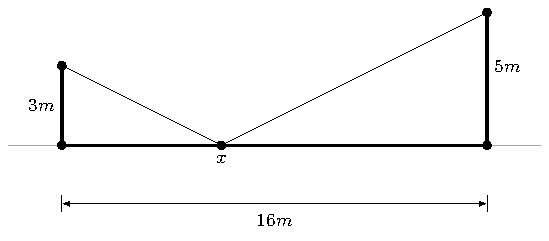
\includegraphics{figuras/postes.pdf}
        \caption{Postes y cable del ejercicio~\ref{ej:314}.}
        \label{fig:5.30}
    \end{figure}

    \section{Regla de L'Hôpital}\label{sec:lhopital}

    Supongamos que queremos calcular un límite de la forma
    \begin{equation}\label{eq:5.30}
        \lim_{x\to p}\frac{f(x)}{g(x)},
    \end{equation}
    donde $\lim_{x\to p}f(x)=0$ y $\lim_{x\to p}g(x)=0$. Notemos que en esta situación
    no podemos aplicar el inciso (d) del álgebra de límites, pues el límite del
    denominador es cero. Notemos también que la derivada de una función es un
    límite de este tipo. Para ser más precisos, recordemos que si $f$ es derivable
    en $p$, entonces $f'(p)$ está dada por
    \begin{equation}\label{eq:5.31}
        \lim_{h\to 0}\frac{f(p+h)-f(p)}{h},
    \end{equation}
    y tanto el límite (cuando $h\to 0$) del numerador como del denominador de la
    fracción de \eqref{eq:5.31} son cero. Dada la importancia de encontrar la derivada de
    una función, es útil el disponer de herramientas que permitan calcular límites
    de la forma \eqref{eq:5.30}, donde $\lim_{x\to p}f(x)=0$ y $\lim_{x\to p}g(x)=0$. Una de esas
    herramientas es la regla o fórmula de L'Hôpital.

    \subsection{Formas Indeterminadas}

    Supongamos que queremos calcular
    \begin{equation}\label{eq:5.32}
        \lim_{x\to p}\frac{f(x)}{g(x)}
    \end{equation}
    y que
    \begin{equation}\label{eq:5.33}
        \frac{\lim_{x\to p}f(x)}{\lim_{x\to p}g(x)}
    \end{equation}
    toma la forma $L/0$ (que carece de sentido), donde $L$ es un número real extendido.
    En este caso, como comentamos anteriormente, no se puede aplicar
    el inciso (d) del álgebra de límites (reales o infinitos), pues el límite del denominador
    es cero. Si $L\neq 0$, por el ejercicio~\ref{ej:176}, sabemos que el límite \eqref{eq:5.32}
    puede ser $\infty$, $-\infty$ o no existir (ni como límite real, ni como límite infinito).
    El único caso en que no sabemos lo que sucede con el límite \eqref{eq:5.32} es cuando
    \eqref{eq:5.33} toma la forma $0/0$. Esta es la razón por la cual al símbolo $0/0$ se le
    llama \textit{forma indeterminada}\index{formas indeterminadas}. Por una razón análoga, a $\pm\infty/\pm\infty$ y $\pm\infty/\mp\infty$
    también se les llama formas indeterminadas. De manera similar, si queremos
    calcular límites de la forma
    \begin{equation*}
        \lim_{x\to p}f(x)g(x)
    \end{equation*}
    se pueden presentar las formas indeterminadas $0\cdot\pm\infty$ o $\pm\infty\cdot 0$, y si queremos
    calcular límites de la forma
    \begin{equation*}
        \lim_{x\to p}(f(x)+g(x))
    \end{equation*}
    se pueden presentar las formas indeterminadas $\infty-\infty$ o $-\infty+\infty$.

    \subsection{Regla de L'Hôpital}

    Como consecuencia del teorema del valor medio generalizado obtenemos
    el resultado siguiente.

    \begin{proposicion}[Regla de L'Hôpital]\label{prop:67}
        \index{regla de l'hopital@regla de L'Hôpital}Supongamos que $f$ y $g$ son funciones
        derivables en un intervalo abierto $I$ que contiene a $p$, excepto posiblemente
        en $p$, y que $g'(x)\neq 0$, $x\in I\backslash\{p\}$. Si
        \begin{equation}\label{eq:5.34}
            \frac{\lim_{x\to p}f(x)}{\lim_{x\to p}g(x)}
        \end{equation}
        toma la forma indeterminada $0/0$ y existe
        \begin{equation}\label{eq:5.35}
            \lim_{x\to p}\frac{f'(x)}{g'(x)}
        \end{equation}
        (como límite real o como límite infinito), entonces
        \begin{equation*}
            \lim_{x\to p}\frac{f(x)}{g(x)}=\lim_{x\to p}\frac{f'(x)}{g'(x)}.
        \end{equation*}
    \end{proposicion}

    \begin{proof}
        Supongamos que \eqref{eq:5.35} es un número real $L$, la prueba en
        el caso en que \eqref{eq:5.35} es $\pm\infty$ es similar. Primero notemos que $f$ y $g$ pueden
        no estar definidas en $p$. Definiendo o redefiniendo si es necesario $f$ y $g$ en $p$,
        podemos suponer que $f(p)=g(p)=0$ y, en consecuencia, que $f$ y $g$ son
        continuas en $p$. Notemos también que $g(x)\neq 0$ si $x\in I\backslash\{p\}$ (¿por qué?).
        Dado $x\in I$ con $x\neq p$, por el teorema del valor medio generalizado, existe $c_{x}$
        entre $x$ y $p$ tal que
        \begin{equation*}
            (f(x)-f(p))g'(c_{x})=f'(c_{x})(g(x)-g(p)).
        \end{equation*}
        Así,
        \begin{equation*}
            \frac{f(x)}{g(x)}=\frac{f'(c_{x})}{g'(c_{x})}.
        \end{equation*}
        Como $c_{x}\to p$ cuando $x\to p$, intuitivamente se debe cumplir que
        \begin{equation}\label{eq:5.36}
            \lim_{x\to p}\frac{f'(c_{x})}{g'(c_{x})}=\lim_{x\to p}\frac{f'(x)}{g'(x)}.
        \end{equation}
        En efecto, probaremos que \eqref{eq:5.36} se cumple, de lo cual obtendremos lo afirmado.
        Sea $\epsilon>0$. Existe $\delta>0$ tal que
        \begin{equation}\label{eq:5.37}
            \text{si }x\in I\text{ y }0<|x-p|<\delta,\text{ entonces }\left|\frac{f'(x)}{g'(x)}-L\right|<\epsilon.
        \end{equation}
        Puesto que $c_{x}$ está entre $x$ y $p$, resulta que si $x\in I$ y $0<|x-p|<\delta$, entonces
        $0<|c_{x}-p|<\delta$ y, en consecuencia, por \eqref{eq:5.37},
        \begin{equation*}
            \left|\frac{f'(c_{x})}{g'(c_{x})}-L\right|<\epsilon,
        \end{equation*}
        de lo cual obtenemos \eqref{eq:5.36}.
    \end{proof}

    La regla de L'Hôpital, con sus respectivas modificaciones, sigue siendo
    válida si en lugar de considerar límites cuando $x\to p$ se consideran límites
    laterales (esto debe ser claro si modificamos la demostración de la regla de
    L'Hôpital para considerar límites laterales). Más aún, sigue siendo válida si
    en lugar de considerar límites cuando $x\to p$ se consideran límites al infinito
    (véase el ejercicio~\ref{ej:316}).

    Como caso particular del resultado siguiente, consecuencia también del
    teorema del valor medio generalizado, obtenemos que la regla de L'Hôpital
    también es válida si en \eqref{eq:5.34} en lugar de la forma indeterminada $0/0$ aparecen
    las formas indeterminadas $\pm\infty/\pm\infty$ o $\pm\infty/\mp\infty$.

    \begin{proposicion}\label{prop:68}
        Supongamos que $f$ y $g$ son funciones derivables en un intervalo
        abierto $I$ que contiene a $p$, excepto posiblemente en $p$, y que $g'(x)\neq 0$,
        $x\in I\backslash\{p\}$. Si
        \begin{equation}\label{eq:5.38}
            \lim_{x\to p}g(x)=\pm\infty
        \end{equation}
        y existe
        \begin{equation}\label{eq:5.39}
            \lim_{x\to p}\frac{f'(x)}{g'(x)}
        \end{equation}
        (como límite real o como límite infinito), entonces
        \begin{equation}\label{eq:5.40}
            \lim_{x\to p}\frac{f(x)}{g(x)}=\lim_{x\to p}\frac{f'(x)}{g'(x)}.
        \end{equation}
    \end{proposicion}

    \begin{proof}
        Por \eqref{eq:5.38} podemos suponer que $g(x)\neq 0$ si $x\in I\backslash\{p\}$.
        Supongamos primero que \eqref{eq:5.39} es un número real $L$. Sea $\epsilon>0$. Existe $\delta>0$
        tal que
        \begin{equation}\label{eq:5.41}
            \text{si }x\in I\text{ y }0<|x-p|<\delta,\text{ entonces }\left|\frac{f'(x)}{g'(x)}-L\right|<\frac{\epsilon}{2}.
        \end{equation}
        Fijemos $y\in I$ tal que $0<y-p<\delta$ y tomemos $x\in I$ con $p<x<y$. Por el
        teorema del valor medio generalizado, existe $c_{xy}\in(x,y)$ tal que
        \begin{equation*}
            (f(x)-f(y))g'(c_{xy})=f'(c_{xy})(g(x)-g(y)).
        \end{equation*}
        Así,
        \begin{equation}\label{eq:5.42}
            \frac{f(x)-f(y)}{g(x)-g(y)}=\frac{f'(c_{xy})}{g'(c_{xy})}
        \end{equation}
        (de las hipótesis y del teorema del valor intermedio para derivadas (teorema~\ref{teo:6})
        obtenemos que $g'$ no cambia de signo en los intervalos que resultan al
        «extraer» de $I$ el punto $p$, por lo cual $g$ es creciente o decreciente en tales
        intervalos y, en consecuencia, $g(x)-g(y)\neq 0$). Observemos que \eqref{eq:5.41} y
        \eqref{eq:5.42} implican que
        \begin{equation*}
            \left|\frac{f(x)-f(y)}{g(x)-g(y)}\right|\leq\left|\frac{f'(c_{xy})}{g'(c_{xy})}-L\right|+|L|\leq\frac{\epsilon}{2}+|L|,\ \ p<x<y,
        \end{equation*}
        es decir, el cociente del lado izquierdo de \eqref{eq:5.42} está acotado si $p<x<y$.
        Por \eqref{eq:5.41} y \eqref{eq:5.42} también obtenemos que
        \begin{align}
            \left|\frac{f(x)}{g(x)}-L\right|&\leq\left|\frac{f(x)}{g(x)}-\frac{f(x)-f(y)}{g(x)-g(y)}\right|+\left|\frac{f'(c_{xy})}{g'(c_{xy})}-L\right|\notag\\
            &<\left|\frac{f(x)}{g(x)}-\frac{f(x)-f(y)}{g(x)-g(y)}\right|+\frac{\epsilon}{2},\ \ p<x<y.\label{eq:5.43}
        \end{align}
        Mostraremos ahora que
        \begin{equation}\label{eq:5.44}
            \lim_{x\to p^{+}}\frac{f(x)}{g(x)}-\frac{f(x)-f(y)}{g(x)-g(y)}=0,
        \end{equation}
        lo cual nos permitirá concluir lo deseado. Efectivamente, puesto que
        \begin{align*}
            \frac{f(x)}{g(x)}-\frac{f(x)-f(y)}{g(x)-g(y)}&=\frac{g(x)f(y)-f(x)g(y)}{g(x)(g(x)-g(y))}\\
            &=\frac{f(y)}{g(x)}-\frac{g(y)}{g(x)}\frac{f(x)-f(y)}{g(x)-g(y)},
        \end{align*}
        del hecho de que el cociente del lado izquierdo de \eqref{eq:5.42} está acotado si
        $p<x<y$ y de que $\lim_{x\to p}g(x)=\pm\infty$ obtenemos \eqref{eq:5.44}, de lo cual, junto
        con \eqref{eq:5.43}, resulta que
        \begin{equation*}
            \lim_{x\to p^{+}}\frac{f(x)}{g(x)}=L.
        \end{equation*}
        De forma similar se muestra que
        \begin{equation*}
            \lim_{x\to p^{-}}\frac{f(x)}{g(x)}=L,
        \end{equation*}
        de lo cual resulta \eqref{eq:5.40}. Supongamos ahora que \eqref{eq:5.39} es $\infty$, la prueba en el
        caso en que \eqref{eq:5.39} es $-\infty$ es similar. Sea $M>0$. Existe $\eta>0$ tal que
        \begin{equation}\label{eq:5.45}
            \text{si }x\in I\text{ y }0<|x-p|<\eta,\text{ entonces }\frac{f'(x)}{g'(x)}>2(M+1).
        \end{equation}
        Fijemos $y\in I$ tal que $0<y-p<\eta$ y tomemos $x\in I$ con $p<x<y$. Por el
        teorema del valor medio generalizado, existe $c_{xy}\in(x,y)$ tal que
        \begin{equation*}
            (f(x)-f(y))g'(c_{xy})=f'(c_{xy})(g(x)-g(y)).
        \end{equation*}
        Así,
        \begin{equation}\label{eq:5.46}
            \frac{f(x)}{g(x)}=\frac{f'(c_{xy})}{g'(c_{xy})}\left(1-\frac{g(y)}{g(x)}\right)+\frac{f(y)}{g(x)}.
        \end{equation}
        Por \eqref{eq:5.38}, existe $0<\delta<y-p$ tal que si $0<x-p<\delta$, entonces
        \begin{equation}\label{eq:5.47}
            \left|\frac{g(y)}{g(x)}\right|<\frac{1}{2}\ \ \text{y}\ \ \left|\frac{f(y)}{g(x)}\right|<1.
        \end{equation}
        De \eqref{eq:5.45}, \eqref{eq:5.46} y \eqref{eq:5.47} obtenemos que si $0<x-p<\delta$, entonces
        \begin{align*}
            \frac{f(x)}{g(x)}&>2(M+1)\frac{1}{2}-1\\
            &=M,
        \end{align*}
        por lo cual
        \begin{equation*}
            \lim_{x\to p^{+}}\frac{f(x)}{g(x)}=\infty.
        \end{equation*}
        De forma similar se muestra que
        \begin{equation*}
            \lim_{x\to p^{-}}\frac{f(x)}{g(x)}=\infty,
        \end{equation*}
        de lo cual resulta \eqref{eq:5.40}.
    \end{proof}

    La proposición~\ref{prop:68}, con sus respectivas modificaciones, sigue siendo válida
    si en lugar de considerar límites cuando $x\to p$ se consideran límites laterales
    (esto debe ser claro si modificamos la demostración de la proposición~\ref{prop:68}
    para considerar límites laterales). Más aún, sigue siendo válida si en lugar
    de considerar límites cuando $x\to p$ se consideran límites al infinito (véase el
    ejercicio~\ref{ej:317}).

    Veamos algunos ejemplos.

    \subtitulo{Límites con la Forma Indeterminada $\boldsymbol{0/0}$}

    \begin{ejemplo}[Forma indeterminada $0/0$]\label{ejm:99}
        Calcula
        \begin{equation*}
            \lim_{x\to -1}\frac{x^{2}+4x+3}{x+1}.
        \end{equation*}

        \textbf{Solución.} Notemos que
        \begin{equation*}
            \frac{\lim_{x\to -1}\left(x^{2}+4x+3\right)}{\lim_{x\to -1}(x+1)}
        \end{equation*}
        toma la forma indeterminada $0/0$. Luego, por la regla de L'Hôpital resulta
        que
        \begin{equation*}
            \lim_{x\to -1}\frac{x^{2}+4x+3}{x+1}=\lim_{x\to -1}\frac{2x+4}{1}=2.\finej
        \end{equation*}
    \end{ejemplo}

    \begin{ejemplo}[Forma indeterminada $0/0$]\label{ejm:100}
        Calcula
        \begin{equation*}
            \lim_{x\to 0}\frac{\sin(x)}{x}.
        \end{equation*}

        \textbf{Solución.} Recordemos que ya calculamos este límite usando el lema del
        sándwich en la sección de límites reales. Notemos que
        \begin{equation*}
            \frac{\lim_{x\to 0}\sin(x)}{\lim_{x\to 0}x}
        \end{equation*}
        toma la forma indeterminada $0/0$. Luego, por la regla de L'Hôpital resulta
        que
        \begin{equation*}
            \lim_{x\to 0}\frac{\sin(x)}{x}=\lim_{x\to 0}\frac{\cos(x)}{1}=1,
        \end{equation*}
        como habíamos calculado.
    \end{ejemplo}

    \begin{ejemplo}[Forma indeterminada $0/0$]\label{ejm:101}
        Calcula
        \begin{equation*}
            \lim_{x\to 0}\frac{\sin(5x)}{\sin(3x)}.
        \end{equation*}

        \textbf{Solución.} Notemos que
        \begin{equation*}
            \frac{\lim_{x\to 0}\sin(5x)}{\lim_{x\to 0}\sin(3x)}
        \end{equation*}
        toma la forma indeterminada $0/0$. Luego, por la regla de L'Hôpital resulta
        que
        \begin{equation*}
            \lim_{x\to 0}\frac{\sin(5x)}{\sin(3x)}=\lim_{x\to 0}\frac{5\cos(5x)}{3\cos(3x)}=\frac{5}{3}.\finej
        \end{equation*}
    \end{ejemplo}

    \begin{ejemplo}[Uso repetido de la Regla de L'Hôpital]\label{ejm:102}
        Calcula
        \begin{equation*}
            \lim_{x\to 0}\frac{1-\cos(x)}{x^{2}}.
        \end{equation*}

        \textbf{Solución.} Notemos que
        \begin{equation*}
            \frac{\lim_{x\to 0}1-\cos(x)}{\lim_{x\to 0}x^{2}}
        \end{equation*}
        toma la forma indeterminada $0/0$. Luego, por la regla de L'Hôpital resulta
        que
        \begin{equation*}
            \lim_{x\to 0}\frac{1-\cos(x)}{x^{2}}=\lim_{x\to 0}\frac{\sin(x)}{2x},
        \end{equation*}
        siempre y cuando este último límite exista. Notemos ahora que
        \begin{equation*}
            \frac{\lim_{x\to 0}\sin(x)}{\lim_{x\to 0}2x}
        \end{equation*}
        también toma la forma indeterminada $0/0$. Aplicando nuevamente la regla
        de L'Hôpital resulta que
        \begin{equation*}
            \lim_{x\to 0}\frac{\sin(x)}{2x}=\lim_{x\to 0}\frac{\cos(x)}{2}=\frac{1}{2}.
        \end{equation*}
        Por lo tanto,
        \begin{equation*}
            \lim_{x\to 0}\frac{1-\cos(x)}{x^{2}}=\frac{1}{2}.\finej
        \end{equation*}
    \end{ejemplo}

    \subtitulo{Límites con Otras Formas Indeterminadas}

    \begin{ejemplo}[Forma indeterminada $\infty/\infty$]\label{ejm:103}
        Calcula
        \begin{equation}\label{eq:5.48}
            \lim_{x\to\infty}\frac{\ln(x)}{x}.
        \end{equation}

        \textbf{Solución.} Notemos que
        \begin{equation*}
            \frac{\lim_{x\to\infty}\ln(x)}{\lim_{x\to\infty}x}
        \end{equation*}
        toma la forma indeterminada $\infty/\infty$. Luego, por la regla de L'Hôpital resulta
        que
        \begin{equation*}
            \lim_{x\to\infty}\frac{\ln(x)}{x}=\lim_{x\to\infty}\frac{1/x}{1}=0.\finej
        \end{equation*}
    \end{ejemplo}

    Como una aplicación interesante de la regla de L'Hôpital, probaremos que
    la función exponencial «crece más rápido» que cualquier polinomio.

    \begin{ejemplo}[La función exponencial «crece más rápido» que cualquier polinomio]\label{ejm:104}
        Sea $P(x)$ un polinomio. Entonces
        \begin{equation}\label{eq:5.49}
            \lim_{x\to\infty}\frac{P(x)}{e^{x}}=0.
        \end{equation}
        En efecto, por el álgebra de límites al infinito, basta probar el caso en que
        $P(x)=x^{n}$. Al aplicar la regla de L'Hôpital $n$-veces (con la forma $\infty/\infty$)
        obtenemos que
        \begin{equation*}
            \lim_{x\to\infty}\frac{P(x)}{e^{x}}=\lim_{x\to\infty}\frac{x^{n}}{e^{x}}=\lim_{x\to\infty}\frac{nx^{n-1}}{e^{x}}=\cdots=\lim_{x\to\infty}\frac{n!}{e^{x}}=0.
        \end{equation*}
        La ecuación \eqref{eq:5.49} indica que la función exponencial «crece más rápido» que
        el polinomio $P(x)$, aunque $\lim_{x\to\infty}P(x)=\pm\infty$ para el caso de polinomios
        no constantes.
    \end{ejemplo}

    \begin{ejemplo}[Forma indeterminada $\infty\cdot 0$]\label{ejm:105}
        Calcula
        \begin{equation*}
            \lim_{x\to\infty}xe^{1-x}.
        \end{equation*}

        \textbf{Solución.} Notemos que
        \begin{equation*}
            \left(\lim_{x\to\infty}x\right)\left(\lim_{x\to\infty}e^{1-x}\right)
        \end{equation*}
        toma la forma indeterminada $\infty\cdot 0$. Lo que haremos será expresar $xe^{1-x}$ de
        otra manera para poder emplear la regla de L'Hôpital. Puesto que
        \begin{equation*}
            xe^{1-x}=\frac{x}{e^{x-1}}
        \end{equation*}
        y
        \begin{equation*}
            \frac{\lim_{x\to\infty}x}{\lim_{x\to\infty}e^{x-1}}
        \end{equation*}
        toma la forma indeterminada $\infty/\infty$, al aplicar la regla de L'Hôpital resulta
        que
        \begin{equation*}
            \lim_{x\to\infty}xe^{1-x}=\lim_{x\to\infty}\frac{x}{e^{x-1}}=\lim_{x\to\infty}\frac{1}{e^{x-1}}=0.\finej
        \end{equation*}
    \end{ejemplo}

    En general, como en el ejemplo anterior, cuando queramos calcular el límite
    de un producto de funciones que conduce a una forma indeterminada, se
    intenta expresar dicho producto de otra manera para poder usar la regla de
    L'Hôpital.

    Finalmente, es importante señalar que no existe un criterio similar a la
    regla de L'Hôpital para calcular el límite de una suma de funciones $f(x)+
    g(x)$ que produce una forma indeterminada de la forma $\infty-\infty$ o de la forma
    $-\infty+\infty$. En tales casos se procede utilizando las propiedades particulares
    de las funciones $f$ y $g$.

    \par\avoidorphan{6}\subsection*{Ejercicios}

    \begin{enumerate}[label=\arabic*.]
        \item Calcula los límites siguientes:
        \begin{multicols}{2}
        \begin{enumerate}[nosep]
            \item $\lim_{x\to 1}\frac{x^{3}+x^{2}-2}{x-1}$.
            \item $\lim_{x\to 0}\frac{3x^{2}+2x}{e^{x}-1}$.
            \item $\lim_{x\to\infty}\frac{\ln(x)}{x+1}$.
            \item $\lim_{x\to 0^{+}}\sin(x)x^{-1/2}$.
            \item $\lim_{h\to 0}\frac{\sqrt{1+h}-1}{h}$.
        \end{enumerate}
        \end{multicols}
    \end{enumerate}

    \begin{ejercicio}\label{ej:315}
        Supón que $f$ y $g$ son funciones definidas en un intervalo abierto
        $I$ que contiene a $p$ tales que $f(p)=g(p)=0$ y $g(x)\neq 0$ si $x\in I\backslash\{p\}$.
        Prueba que si $f$ y $g$ son derivables en $p$ y $g'(p)\neq 0$, entonces
        \begin{equation*}
            \lim_{x\to p}\frac{f(x)}{g(x)}=\frac{f'(p)}{g'(p)}.
        \end{equation*}
    \end{ejercicio}

    \begin{ejercicio}\label{ej:316}
        Prueba que la regla de L'Hôpital (proposición~\ref{prop:67}), con sus
        respectivas modificaciones, sigue siendo válida si en lugar de considerar límites
        cuando $x\to p$ se consideran límites al infinito. \sugerencia Trata de utilizar
        el ejercicio~\ref{ej:167} para transformar el problema dado a uno donde puedas aplicar
        la regla de L'Hôpital (proposición~\ref{prop:67}) con límites laterales.
    \end{ejercicio}

    \begin{ejercicio}\label{ej:317}
        Prueba que la proposición~\ref{prop:68}, con sus respectivas modificaciones,
        sigue siendo válida si en lugar de considerar límites cuando $x\to p$ se
        consideran límites al infinito. \sugerencia Trata de utilizar el ejercicio~\ref{ej:167}
        para transformar el problema dado a uno donde puedas aplicar la proposición~\ref{prop:68}
        con límites laterales.
    \end{ejercicio}

    \section{Polinomios de Taylor}

    En esta sección, «aproximaremos» una función varias veces derivable en
    un punto $x_{0}$ por ciertos polinomios, los llamados polinomios de Taylor.

    \begin{definicion}[Polinomios de Taylor]\label{def:55}
        Sea $f$ una función $n$-veces derivable
        en $x_{0}$. Definimos el \textit{polinomio de Taylor de $f$ de orden $n$ centrado en $x_{0}$}\index{polinomios de taylor de una funcion@polinomios de Taylor de una función}
        como el polinomio $P$ de grado menor o igual a $n$ centrado en $x_{0}$ tal que
        \begin{equation}\label{eq:5.50}
            P^{(k)}(x_{0})=f^{(k)}(x_{0}),\ \ k=0,1,\ldots,n,
        \end{equation}
        es decir, como el polinomio
        \begin{equation*}
            P(x)=f(x_{0})+\frac{f^{(1)}(x_{0})}{1!}(x-x_{0})+\cdots+\frac{f^{(n)}(x_{0})}{n!}(x-x_{0})^{n}.
        \end{equation*}
        Denotaremos a $P$ como $P^{f}_{n,x_{0}}$. Definimos el \textit{polinomio de Maclaurin de $f$ de
        orden $n$}\index{polinomios de maclaurin de una funcion@polinomios de Maclaurin de una función} como el polinomio de Taylor de $f$ de orden $n$ centrado en $0$.
    \end{definicion}

    Puesto que un polinomio está determinado por sus coeficientes, entonces
    $P^{f}_{n,x_{0}}$ es único (véase el ejercicio~\ref{ej:318}). Por otra parte, si $f$ es un polinomio
    de grado $n$ centrado en $x_{0}$, es decir, si
    \begin{equation*}
        f(x)=a_{0}+a_{1}(x-x_{0})+a_{2}(x-x_{0})^{2}+\cdots+a_{n}(x-x_{0})^{n},
    \end{equation*}
    entonces no es difícil mostrar que
    \begin{equation*}
        a_{k}=\frac{f^{(k)}(x_{0})}{k!},
    \end{equation*}
    por lo cual, en este caso, $f$ y $P^{f}_{n,x_{0}}$ coinciden.

    \begin{ejemplo}[Polinomios de Taylor de $e^{x}$ centrados en $0$]\label{ejm:106}
        Sea $f(x)=
        e^{x}$. La función exponencial $e^{x}$ tiene derivadas de todos los ordenes, así que
        el polinomio de Taylor $P^{f}_{n,0}$ existe para toda $n$; veamos cual es su expresión.
        Puesto que
        \begin{equation*}
            f^{(k)}(x)=e^{x},\ \ k\in\N_{0},
        \end{equation*}
        entonces
        \begin{equation*}
            f^{(k)}(0)=1,\ \ k\in\N_{0}.
        \end{equation*}
        En consecuencia, el polinomio de Taylor de orden $n$ centrado en $0$ de la
        función exponencial es
        \begin{align*}
            P^{f}_{n,0}(x)&=f(0)+\frac{f^{(1)}(0)}{1!}x+\cdots+\frac{f^{(n)}(0)}{n!}x^{n}\\
            &=1+\frac{x}{1!}+\cdots+\frac{x^{n}}{n!}.
        \end{align*}
        La figura~\ref{fig:5.31} muestra la gráfica de la función exponencial y de sus polinomios
        de Taylor $P^{f}_{n,0}$ para $n=1,2,3$.
    \end{ejemplo}

    \begin{figure}[H]
        \centering
        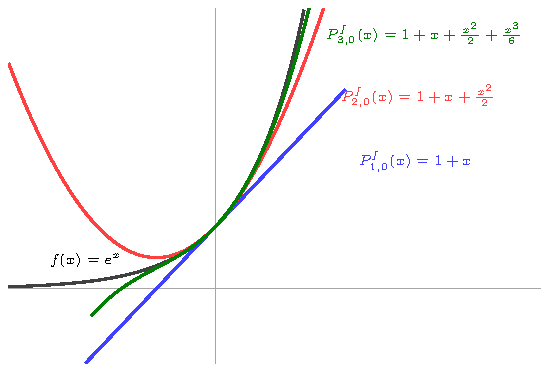
\includegraphics{figuras/taylor-exponencial.pdf}
        \caption{La función exponencial y sus polinomios de Taylor $P^{f}_{n,0}$ para $n=1,2,3$.}
        \label{fig:5.31}
    \end{figure}

    Sea $f$ una función $n$-veces derivable en $x_{0}$. Puesto que el polinomio de
    Taylor $P^{f}_{n,x_{0}}$ cumple \eqref{eq:5.50}, entonces, intuitivamente, $P^{f}_{n,x_{0}}(x)$ es una «buena
    aproximación» de $f(x)$ para $x$ «cerca» de $x_{0}$. Por ejemplo, la gráfica del
    polinomio de Taylor
    \begin{equation}\label{eq:5.51}
        P^{f}_{1,x_{0}}(x)=f(x_{0})+f^{(1)}(x_{0})(x-x_{0})
    \end{equation}
    es la recta tangente a la gráfica de $f$ en el punto $(x_{0},f(x_{0}))$ (recuérdese la
    interpretación geométrica de la derivada) y, en consecuencia, $P^{f}_{1,x_{0}}(x)$ «aproxima
    suficientemente bien» a $f(x)$ cuando $x$ es «cercana» a $x_{0}$. La proposición
    siguiente muestra que, efectivamente, el polinomio de Taylor $P^{f}_{n,x_{0}}(x)$ es una
    «buena aproximación» de $f(x)$ para $x$ «cerca» de $x_{0}$.

    \begin{proposicion}\label{prop:69}
        Sea $f$ una función $n$-veces derivable en $x_{0}$. Entonces
        \begin{equation}\label{eq:5.52}
            \lim_{x\to x_{0}}\frac{f(x)-P^{f}_{n,x_{0}}(x)}{(x-x_{0})^{n}}=0.
        \end{equation}
    \end{proposicion}

    \begin{proof}
        Notemos primero que el límite \eqref{eq:5.52} toma la forma indeterminada
        $0/0$ y que podemos aplicar la regla de L'Hôpital. Más aún, notemos
        que podemos aplicar $n-1$ veces tal regla al límite \eqref{eq:5.52}. Al aplicar entonces
        $n-1$ veces la regla de L'Hôpital a \eqref{eq:5.52} obtenemos que
        \begin{align*}
            \lim_{x\to x_{0}}\frac{f(x)-P^{f}_{n,x_{0}}(x)}{(x-x_{0})^{n}}&=\lim_{x\to x_{0}}\frac{f^{(n-1)}(x)-f^{(n-1)}(x_{0})-f^{(n)}(x_{0})(x-x_{0})}{n!(x-x_{0})}\\
            &=\frac{1}{n!}\left[\lim_{x\to x_{0}}\frac{f^{(n-1)}(x)-f^{(n-1)}(x_{0})}{x-x_{0}}-f^{(n)}(x_{0})\right]\\
            &=\frac{1}{n!}\left[f^{(n)}(x_{0})-f^{(n)}(x_{0})\right] &&\text{(véase el ejercicio~\ref{ej:231})}\\
            &=0.\qedhere
        \end{align*}
    \end{proof}

    Observemos que el límite \eqref{eq:5.52} nos indica que $f(x)-P^{f}_{n,x_{0}}(x)$ se «aproxima»
    a cero «más rápido» que $(x-x_{0})^{n}$ cuando $x$ tiende a $x_{0}$. Por \eqref{eq:5.52}
    se dice que $f$ y su polinomio de Taylor $P^{f}_{n,x_{0}}$ son iguales hasta el orden $n$ en
    $x_{0}$; más en general, tenemos la definición siguiente.

    \begin{definicion}[Funciones iguales hasta el orden $n$ en $x_{0}$]\label{def:56}
        \index{funciones iguales hasta el orden n@funciones iguales hasta el orden $n$}Sean $f$ y $g$
        funciones definidas en un intervalo abierto que contiene a $x_{0}$. Diremos que $f$
        y $g$ son \textit{iguales hasta el orden $n$} en $x_{0}$ si
        \begin{equation*}
            \lim_{x\to x_{0}}\frac{f(x)-g(x)}{(x-x_{0})^{n}}=0.
        \end{equation*}
    \end{definicion}

    Notemos que si $f\sim g$ denota que $f$ y $g$ son iguales hasta el orden $n$ en $x_{0}$,
    entonces $\sim$ es una relación de equivalencia, es decir, $\sim$ es reflexiva ($f\sim f$),
    simétrica (si $f\sim g$, entonces $g\sim f$) y transitiva (si $f\sim g$ y $g\sim h$, entonces
    $f\sim h$).

    Como consecuencia inmediata de la proposición siguiente obtenemos que
    el polinomio de Taylor $P^{f}_{n,x_{0}}$ es el único polinomio de grado menor o igual a
    $n$ centrado en $x_{0}$ que cumple \eqref{eq:5.52}.

    \begin{proposicion}\label{prop:70}
        Sean $P$ y $Q$ polinomios de grado menor o igual a $n$ centrados
        en $x_{0}$. Si $P$ y $Q$ son iguales hasta el orden $n$ en $x_{0}$, entonces $P=Q$.
    \end{proposicion}

    \begin{proof}
        Supongamos que
        \begin{equation*}
            P(x)=a_{0}+a_{1}(x-x_{0})+a_{2}(x-x_{0})^{2}+\cdots+a_{n}(x-x_{0})^{n}
        \end{equation*}
        y
        \begin{equation*}
            Q(x)=b_{0}+b_{1}(x-x_{0})+b_{2}(x-x_{0})^{2}+\cdots+b_{n}(x-x_{0})^{n}.
        \end{equation*}
        Deseamos mostrar que $a_{i}=b_{i}$, $i=0,1,\ldots,n$. Como $P$ y $Q$ son iguales hasta
        el orden $n$ en $x_{0}$, entonces
        \begin{equation}\label{eq:5.53}
            \lim_{x\to x_{0}}\frac{P(x)-Q(x)}{(x-x_{0})^{n}}=0.
        \end{equation}
        Si $|x-x_{0}|<1$, entonces $|x-x_{0}|^{n}\leq|x-x_{0}|^{i}$, $i=0,1,\ldots,n$, por lo cual
        \begin{equation}\label{eq:5.54}
            \left|\frac{P(x)-Q(x)}{(x-x_{0})^{i}}\right|\leq\left|\frac{P(x)-Q(x)}{(x-x_{0})^{n}}\right|,\ \ i=0,1,\ldots,n.
        \end{equation}
        De \eqref{eq:5.54} y de \eqref{eq:5.53} obtenemos que
        \begin{equation}\label{eq:5.55}
            a_{0}-b_{0}=\lim_{x\to x_{0}}\frac{P(x)-Q(x)}{(x-x_{0})^{0}}=0.
        \end{equation}
        De \eqref{eq:5.55}, \eqref{eq:5.54} y de \eqref{eq:5.53} obtenemos que
        \begin{equation}\label{eq:5.56}
            a_{1}-b_{1}=\lim_{x\to x_{0}}\frac{P(x)-Q(x)}{(x-x_{0})^{1}}=0.
        \end{equation}
        Continuando de esta manera obtenemos que $a_{i}-b_{i}=0$, $i=0,1,\ldots,n$.
    \end{proof}

    Para estudiar que tan buena es la aproximación del polinomio de Taylor
    $P^{f}_{n,x_{0}}(x)$ a la función $f(x)$, introduzcamos el concepto siguiente.

    \begin{definicion}[Resto]\label{def:57}
        Sea $f$ una función $n$-veces derivable en $x_{0}$. Definimos
        el \textit{resto de $f$ de orden $n$ centrado en $x_{0}$}\index{resto de una funcion@resto de una función}, denotado como $R^{f}_{n,x_{0}}$, mediante
        la ecuación
        \begin{equation*}
            f(x)=P^{f}_{n,x_{0}}(x)+R^{f}_{n,x_{0}}(x).
        \end{equation*}
    \end{definicion}

    Mientras más pequeño sea el resto $R^{f}_{n,x_{0}}(x)$, mejor será la aproximación
    del polinomio de Taylor $P^{f}_{n,x_{0}}(x)$ a la función $f(x)$. El teorema siguiente nos
    proporciona una forma del resto, llamada \textit{forma de Lagrange del resto}\index{forma de Lagrange del resto},\footnote{En \cite{nunez2020calculoII} estudiaremos otras formas del resto, después de que hayamos visto la integral.} que
    nos permitirá su estimación.

    \begin{teorema}[de Taylor]\label{teo:9}
        \index{teorema de Taylor}Sean $n\in\N_{0}$ y $f$ una función $(n+1)$-veces derivable
        en un intervalo abierto $I$ que contiene a $x_{0}$. Si $x\in I\backslash\{x_{0}\}$, entonces
        existe $c$ entre $x$ y $x_{0}$ tal que
        \begin{equation}\label{eq:5.57}
            R^{f}_{n,x_{0}}(x)=\frac{f^{(n+1)}(c)}{(n+1)!}(x-x_{0})^{n+1}.
        \end{equation}
        Notemos que si hacemos $n=0$ en \eqref{eq:5.57}, obtenemos el teorema del valor
        medio.
    \end{teorema}

    \begin{proof}
        Sea $x\in I\backslash\{x_{0}\}$. Consideremos a la función auxiliar
        \begin{equation*}
            g(t)=f(t)-P^{f}_{n,x_{0}}(t)-K(t-x_{0})^{n+1},
        \end{equation*}
        donde $K$ es una constante. Para probar lo afirmado deseamos tener que
        $g(x)=0$ y que $K=f^{(n+1)}(c)/(n+1)!$ para algún $c$ entre $x$ y $x_{0}$, así
        que basta tomar
        \begin{equation}\label{eq:5.58}
            K=\frac{f(x)-P^{f}_{n,x_{0}}(x)}{(x-x_{0})^{n+1}}
        \end{equation}
        y probar que
        \begin{equation}\label{eq:5.59}
            K=\frac{f^{(n+1)}(c)}{(n+1)!}
        \end{equation}
        para algún $c$ entre $x$ y $x_{0}$. Tomemos pues $K$ como en \eqref{eq:5.58}. Notemos que
        para probar \eqref{eq:5.59} basta mostrar que $g^{(n+1)}(c)=0$ para algún $c$ entre $x$ y
        $x_{0}$. Observemos que $g^{(k)}(x_{0})=0$, $k=0,1,2,\ldots,n$. Por el teorema del valor
        medio aplicado a $g$, existe $c_{1}$ entre $x$ y $x_{0}$ tal que
        \begin{equation*}
            g(x)-g(x_{0})=g'(c_{1})(x-x_{0}).
        \end{equation*}
        Puesto que $g(x)=g(x_{0})=0$ (recordemos que $g(x)=0$ por la definición de
        $K$), entonces $g'(c_{1})=0$. Por el teorema del valor medio aplicado ahora a $g'$,
        existe $c_{2}$ entre $c_{1}$ y $x_{0}$ tal que
        \begin{equation*}
            g'(c_{1})-g'(x_{0})=g''(c_{2})(c_{1}-x_{0}).
        \end{equation*}
        Puesto que $g'(c_{1})=g'(x_{0})=0$, entonces $g''(c_{2})=0$. Continuando de esta
        manera obtenemos que existe $c$ entre $x$ y $x_{0}$ tal que $g^{(n+1)}(c)=0$.
    \end{proof}

    Como comentamos anteriormente, mientras más pequeño sea el resto
    $R^{f}_{n,x_{0}}(x)$, mejor será la aproximación del polinomio de Taylor $P^{f}_{n,x_{0}}(x)$ a
    la función $f(x)$. Veamos un ejemplo.

    \begin{ejemplo}[Estimación del número $e$]\label{ejm:107}
        Para estimar el número $e$ usaremos
        que $e<3$. Consideremos a la función exponencial $f(x)=e^{x}$. Según
        el teorema de Taylor (con $x_{0}=0$ y $x=1$), existe $c$ entre $0$ y $1$ tal que
        \begin{equation*}
            e=f(1)=P^{f}_{n,0}(1)+R^{f}_{n,0}(1),
        \end{equation*}
        con
        \begin{equation*}
            R^{f}_{n,0}(1)=\frac{f^{(n+1)}(c)}{(n+1)!}(1-0)^{n+1}.
        \end{equation*}
        Puesto que $f^{(n+1)}(c)=e^{c}$, entonces
        \begin{align*}
            \left|R^{f}_{n,0}(1)\right|&=\left|\frac{f^{(n+1)}(c)}{(n+1)!}\right|\\
            &=\left|\frac{e^{c}}{(n+1)!}\right|\\
            &<\frac{e^{1}}{(n+1)!}\\
            &<\frac{3}{(n+1)!}.
        \end{align*}
        Así, si queremos estimar al número $e$ mediante $P^{f}_{n,0}(1)$ con una exactitud de,
        por ejemplo, tres cifras decimales, basta tomar $n$ tal que $3/(n+1)!<1/10^{3}$.
        Tomemos, por ejemplo, $n=6$. Así, con una exactitud de tres cifras decimales,
        tenemos que
        \begin{equation*}
            e\approx P^{f}_{6,0}(1)=1+\frac{1}{1!}+\frac{1}{2!}+\cdots+\frac{1}{6!}=2.71805555555555555.\finej
        \end{equation*}
    \end{ejemplo}

    Es importante señalar que el procedimiento del ejemplo anterior es el que
    usan las calculadoras para obtener, por ejemplo, $\sin(1)$, $\cos(2)$, $\ln(3)$, etc.

    Para terminar esta subsección utilizaremos la proposición~\ref{prop:69} para obtener
    una generalización del criterio de la segunda derivada para encontrar mínimos
    y máximos locales de una función.

    \begin{proposicion}[Criterio de la $n$-ésima derivada]\label{prop:71}
        \index{criterio de la n-esima derivada@criterio de la $n$-ésima derivada}Sea $f$ una función
        $n$-veces derivable en un intervalo abierto $I$ que contiene a $x_{0}$ con\footnote{En \eqref{eq:5.60} se supone que $n\geq 2$, sin embargo, los incisos (f), (g) y (h) de la proposición~\ref{prop:71}
        también son válidos para $n=1$.}
        \begin{equation}\label{eq:5.60}
            f^{(1)}(x_{0})=\cdots=f^{(n-1)}(x_{0})=0.
        \end{equation}
        \begin{enumerate}[nosep]
            \item Si $n$ es par y $f^{(n)}(x_{0})>0$, entonces $f(x_{0})$ es un mínimo local.
            \item Si $n$ es par y $f^{(n)}(x_{0})<0$, entonces $f(x_{0})$ es un máximo local.
            \item Si $n$ es par y $f^{(n)}(x_{0})=0$, entonces puede suceder que $f(x_{0})$ sea mínimo
            local, máximo local o ninguna de las dos cosas.
            \item Si $n$ es par y $f(x_{0})$ es un mínimo local, entonces $f^{(n)}(x_{0})\geq 0$.
            \item Si $n$ es par y $f(x_{0})$ es un máximo local, entonces $f^{(n)}(x_{0})\leq 0$.
            \item Si $n$ es impar y $f^{(n)}(x_{0})\neq 0$, entonces $f(x_{0})$ no es ni mínimo ni máximo
            local.
            \item Si $n$ es impar y $f^{(n)}(x_{0})=0$, entonces puede suceder que $f(x_{0})$ sea mínimo
            local, máximo local o ninguna de las dos cosas.
            \item Si $n$ es impar y $f(x_{0})$ es un mínimo local o máximo local, entonces
            $f^{(n)}(x_{0})=0$.
        \end{enumerate}
    \end{proposicion}

    \begin{proof}
        De \eqref{eq:5.60} obtenemos que
        \begin{equation*}
            P^{f}_{n,x_{0}}(x)=f(x_{0})+\frac{f^{(n)}(x_{0})}{n!}(x-x_{0})^{n}
        \end{equation*}
        y, en consecuencia, por la proposición~\ref{prop:69},
        \begin{equation*}
            \lim_{x\to x_{0}}\frac{f(x)-f(x_{0})}{(x-x_{0})^{n}}-\frac{f^{(n)}(x_{0})}{n!}=0,
        \end{equation*}
        es decir,
        \begin{equation}\label{eq:5.61}
            \lim_{x\to x_{0}}\frac{f(x)-f(x_{0})}{(x-x_{0})^{n}}=\frac{f^{(n)}(x_{0})}{n!}.
        \end{equation}

        (a) Puesto que $f^{(n)}(x_{0})>0$, de \eqref{eq:5.61} obtenemos que existe $\delta>0$ tal que
        \begin{equation}\label{eq:5.62}
            \text{si }x\in(x_{0}-\delta,x_{0}+\delta)\backslash\{x_{0}\},\text{ entonces }\frac{f(x)-f(x_{0})}{(x-x_{0})^{n}}>0,
        \end{equation}
        y como $n$ es par resulta que si $x\in(x_{0}-\delta,x_{0}+\delta)\backslash\{x_{0}\}$, entonces $f(x)-
        f(x_{0})>0$, lo cual señala que $f(x_{0})$ es un mínimo local.

        (b) La prueba de esta afirmación es similar a la del inciso (a).

        (c) Por ejemplo, si $f(x)=x^{n+2}$, $g(x)=-x^{n+2}$ y $r(x)=x^{n+1}$, entonces
        $f^{(1)}(0)=\cdots=f^{(n-1)}(0)=f^{(n)}(0)=0$, $g^{(1)}(0)=\cdots=g^{(n-1)}(0)=
        g^{(n)}(0)=0$, $r^{(1)}(0)=\cdots=r^{(n-1)}(0)=r^{(n)}(0)=0$, $f(0)$ es un mínimo
        local de $f$, $g(0)$ es un máximo local de $g$ y $r(0)$ no es ni mínimo ni máximo
        local de $r$.

        (d) Como $f(x_{0})$ es un mínimo local, existe $\delta>0$ tal que si $x\in
        (x_{0}-\delta,x_{0}+\delta)$, entonces $f(x_{0})\leq f(x)$. Puesto que $n$ es par, de \eqref{eq:5.61}
        resulta entonces que $f^{(n)}(x_{0})\geq 0$.

        (e) La prueba de esta afirmación es similar a la del inciso (d).

        (f) Supongamos que $f^{(n)}(x_{0})>0$, la demostración en el caso en que
        $f^{(n)}(x_{0})<0$ es similar. Como en el inciso (a), existe $\delta>0$ que cumple
        \eqref{eq:5.62}. Por otra parte, como $n$ es impar, entonces $(x-x_{0})^{n}>0$ si $x>x_{0}$ y
        $(x-x_{0})^{n}<0$ si $x<x_{0}$. En consecuencia, $f(x)-f(x_{0})>0$ si $x\in(x_{0},x_{0}+\delta)$
        y $f(x)-f(x_{0})<0$ si $x\in(x_{0}-\delta,x_{0})$. Por lo tanto, $f(x_{0})$ no es ni mínimo
        ni máximo local.

        (g) Por ejemplo, si $f(x)=x^{n+1}$, $g(x)=-x^{n+1}$ y $r(x)=x^{n+2}$, entonces
        $f^{(1)}(0)=\cdots=f^{(n-1)}(0)=f^{(n)}(0)=0$, $g^{(1)}(0)=\cdots=g^{(n-1)}(0)=
        g^{(n)}(0)=0$, $r^{(1)}(0)=\cdots=r^{(n-1)}(0)=r^{(n)}(0)=0$, $f(0)$ es un mínimo
        local de $f$, $g(0)$ es un máximo local de $g$ y $r(0)$ no es ni mínimo ni máximo
        local de $r$.

        (h) Supongamos que $f(x_{0})$ es un mínimo local (la prueba en el caso
        en que $f(x_{0})$ es un máximo local es similar). Así, existe $\delta>0$ tal que si
        $x\in(x_{0}-\delta,x_{0}+\delta)$, entonces $f(x_{0})\leq f(x)$. Como $n$ es impar, entonces
        $(x-x_{0})^{n}>0$ si $x>x_{0}$ y $(x-x_{0})^{n}<0$ si $x<x_{0}$. En consecuencia,
        \begin{equation}\label{eq:5.63}
            \lim_{x\to x_{0}^{-}}\frac{f(x)-f(x_{0})}{(x-x_{0})^{n}}\leq 0
        \end{equation}
        y
        \begin{equation}\label{eq:5.64}
            \lim_{x\to x_{0}^{+}}\frac{f(x)-f(x_{0})}{(x-x_{0})^{n}}\geq 0.
        \end{equation}
        Finalmente, de \eqref{eq:5.63}, \eqref{eq:5.64} y \eqref{eq:5.61} obtenemos que $f^{(n)}(x_{0})=0$.
    \end{proof}

    Notemos que, por ejemplo, si $f(x)=x^{4}$, entonces $f'(0)=f''(0)=0$ y, en
    consecuencia, no podemos aplicar el criterio de la segunda derivada al punto
    crítico $0$ de $f$. Por otra parte, puesto que $f'(0)=f''(0)=f'''(0)=0$ y
    $f^{(4)}(0)>0$, el inciso (a) de la proposición~\ref{prop:71} afirma que $f(0)$ es un mínimo local
    (que por supuesto es el mínimo global de $f$).

    \par\avoidorphan{6}\subsection*{Ejercicios}

    \begin{ejercicio}\label{ej:318}
        Sea $f$ una función $n$-veces derivable en $x_{0}$. Prueba que el
        polinomio de Taylor $P^{f}_{n,x_{0}}$ es único. \sugerencia Recuerda que si un polinomio
        $P$ tiene la forma
        \begin{equation*}
            P(x)=a_{0}+a_{1}(x-x_{0})+a_{2}(x-x_{0})^{2}+\cdots+a_{n}(x-x_{0})^{n},
        \end{equation*}
        entonces
        \begin{equation*}
            a_{k}=\frac{P^{(k)}(x_{0})}{k!},\ \ k=0,1,2,\ldots,n.
        \end{equation*}
    \end{ejercicio}

    \begin{ejercicio}\label{ej:319}
        Expresa los polinomios siguientes como polinomios centrados
        en $1$.
        \begin{multicols}{2}
        \begin{enumerate}[nosep]
            \item $f(x)=5$.
            \item $f(x)=2x+1$.
            \item $f(x)=4x^{2}-9x+6$.
            \item $f(x)=x^{10}-2x^{3}+3x^{2}+7x-11$.
        \end{enumerate}
        \end{multicols}
        \sugerencia Basta con encontrar el polinomio de Taylor de $f$ de grado el
        grado de $f$ centrado en $1$, ¿por qué?
    \end{ejercicio}

    \begin{ejercicio}\label{ej:320}
        Realiza lo siguiente:
        \begin{enumerate}[nosep]
            \item Calcula los polinomios de Taylor centrados en $0$ de la función $\sin(x)$.
            \item Estima el número $\sin(1)$ con una exactitud de tres cifras decimales.
        \end{enumerate}
    \end{ejercicio}

    \begin{ejercicio}\label{ej:321}
        Realiza lo siguiente:
        \begin{enumerate}[nosep]
            \item Calcula los polinomios de Taylor centrados en $0$ de la función $\cos(x)$.
            \item Estima el número $\cos(2)$ con una exactitud de tres cifras decimales.
        \end{enumerate}
        \sugerencia Usa el hecho de que puedes hacer $2^{n}/n!$ tan pequeño como
        quieras tomando $n$ suficientemente grande.
    \end{ejercicio}

    \begin{ejercicio}\label{ej:322}
        Realiza lo siguiente:
        \begin{enumerate}[nosep]
            \item Calcula los polinomios de Taylor centrados en $0$ de la función $\ln(1+x)$.
            \item Estima el número $\ln(3)$ con una exactitud de tres cifras decimales.
        \end{enumerate}
        \sugerencia Usa el hecho de que puedes hacer $2^{n}/n!$ tan pequeño como
        quieras tomando $n$ suficientemente grande.
    \end{ejercicio}


    \backmatter
    \printbibliography[heading=bibintoc,title={Referencias}]
    \printindex

\end{document}
